\documentclass[twoside,nofonts,fancyhdr, 12.5pt]{ctexbook}
\usepackage{indentfirst}
\usepackage{amsmath}
\newtheorem{theorem}{Theorem}
\newcommand{\BlackBox}{\rule{1.5ex}{1.5ex}}  % end of proof
\newenvironment{proof}{\par\noindent{\bf Proof\
}}{\hfill\BlackBox\\[2mm]}
\newtheorem{lemma}[theorem]{Lemma}
\newtheorem{proposition}[theorem]{Proposition}
\newtheorem{remark}[theorem]{Remark}
\newtheorem{corollary}[theorem]{Corollary}
\newtheorem{definition}[theorem]{Definition}
\newtheorem{conjecture}[theorem]{Conjecture}
\newtheorem{axiom}[theorem]{Axiom}

\usepackage{graphicx,booktabs,xcolor,color}
\usepackage{listings}
\usepackage{verbatim}
\usepackage{fancybox,fancyhdr}
\usepackage{xeCJK}
\usepackage{relsize}
\usepackage[a4paper,marginparsep=6mm,marginparwidth=6mm,footskip=3.5pc,centering]{geometry}
\usepackage{subfigure}
\usepackage{tabularx}
\usepackage[toc,page]{appendix}
\usepackage{titlesec}
\usepackage[font=small,labelfont=bf,skip=0pt, aboveskip=0pt, belowskip=0pt,labelsep=space]{caption}

\setlength{\oddsidemargin}{0.0in}
\setlength{\evensidemargin}{0.0in}
\setlength{\topmargin}{0.0in}
\setlength{\topskip}{0.5in}
\setlength{\headheight}{0.5in}
\setlength{\headsep}{0in}
\setlength{\textwidth}{6.5in}
\setlength{\textheight}{8.0in}
\setlength\parindent{2em}
\setlength{\parskip}{0.1in}

\usepackage{hyperref}
\usepackage[figure,table]{hypcap}
\usepackage{natbib}
\setcitestyle{authoryear,round,aysep={,},yysep={,},citesep={;}}
\usepackage{listings}
\definecolor{shadecolor}{rgb}{0.95,0.95,0.95}
\lstset{xrightmargin=0pt,
    basicstyle=\ttfamily,
    commentstyle=\ttfamily,
    numbers=left,
    numberstyle=\tiny,
    backgroundcolor=\color{shadecolor},
    columns=fullflexible,
    showstringspaces=false,
    breaklines=true,
    framerule=0.7pt,
    frameround=tttt,
    captionpos=b,
    xleftmargin=1em,
    xrightmargin=1em,
    aboveskip=1em,
}
\renewcommand{\lstlistingname}{代码}


\CTEXsetup[number={\arabic{chapter}}]{chapter}
\CTEXsetup[format={\Large\bfseries\raggedright}]{section}
\def\cleardoublepage{\clearpage\if@twoside \ifodd\c@page\else
\thispagestyle{empty}%
\hbox{}\newpage\if@twocolumn\hbox{}\newpage\fi\fi\fi}

\titlespacing*{\chapter} {0pt}{50pt}{40pt}
\titlespacing*{\section} {0pt}{3.5ex plus 1ex minus .2ex}{2.3ex plus .2ex}
\titlespacing*{\subsection} {0pt}{3.25ex plus 1ex minus .2ex}{1.5ex plus .2ex}
\titlespacing*{\subsubsection}{0pt}{3.25ex plus 1ex minus .2ex}{1.5ex plus .2ex}

\graphicspath{{fig/}}
\newcommand{\bc}[1]{\textbf{{\color{blue}#1}}}
\newcommand{\PreserveBackslash}[1]{\let\temp=\\#1\let\\=\temp}
\newcolumntype{C}[1]{>{\PreserveBackslash\centering}p{#1}}
\newcolumntype{R}[1]{>{\PreserveBackslash\raggedleft}p{#1}}
\newcolumntype{L}[1]{>{\PreserveBackslash\raggedright}p{#1}}

\pagestyle{fancy}
\fancyhf{} %
\fancyhead[LE,RO]{\bfseries\thepage}
\fancyhead[CO]{\bfseries \nouppercase{\rightmark}}
\fancyhead[CE]{\bfseries \nouppercase{\leftmark}}
\renewcommand{\headrulewidth}{0.5pt}
\renewcommand{\footrulewidth}{0pt}
\addtolength{\headheight}{0.5pt} %
\fancypagestyle{plain}{%
	\fancyhead{} %
	\renewcommand{\headrulewidth}{0pt} %
}

\def\pzh{\CJKglue\vrule height.885ex depth-0.785ex width2em\CJKglue} %%%破折号
\usepackage{marginnote}
\newcommand{\bookpage}[1]{\label{#1}}
\newcommand{\mbookpage}[1]{\label{#1}}

\newcommand{\fun}[1]{\textit{#1}}
\interfootnotelinepenalty=10000
\def\rcode{\expandafter\lstinline[basicstyle={\ttfamily},breaklines=true]}
\usepackage{fancyvrb}
\lstset{escapeinside=`',}
\RecustomVerbatimEnvironment{Verbatim}{Verbatim}{frame=leftline,numbers=left,
	rulecolor=\color{lightgray},framerule=4pt,numbersep=3pt,fontsize=\small}
\fvset{frame=leftline,numbers=left,rulecolor=\color{lightgray},framerule=4pt,
	numbersep=3pt,fontsize=\small}

\widowpenalty=10000
\setlength\parskip{0pt}
\setlength\baselineskip{12pt}	
	


\definecolor{mycolor1}{HTML}{FF6C91}
\definecolor{mycolor2}{HTML}{00C1A9}

\newcommand{\lyxdot}{.}

\usepackage{enumitem}
\setlist{itemsep=0.2ex,partopsep=0pt,parsep=0.2ex,topsep=5pt}

\usepackage{makeidx}
\usepackage{cosmidx}
\def\tcode{\expandafter\lstinline[basicstyle={},breaklines=true]}
\makeindex{terms}
\makeindex{software}
\makeindex{author}
\newcommand{\tindex}[2]{\index{terms}{#1@#2}}
\newcommand{\sindex}[2]{\index{software}{#1@#2}}
\newcommand{\aindex}[2]{\index{author}{#1@#2}}

\renewcommand{\thefootnote}{\scriptsize{\textcircled{\tiny{\arabic{footnote}}}}}
\DeclareGraphicsExtensions{.pdf,.jpg,.png}

\usepackage[section]{placeins}

\renewcommand{\textfraction}{0}
\renewcommand{\topfraction}{1}
\renewcommand{\bottomfraction}{0.99}
\renewcommand{\floatpagefraction}{0.9}
\makeatletter
\setlength{\@fptop}{0pt}
\setlength{\@fpbot}{0pt}
\makeatother

\setCJKmainfont[BoldFont={方正黑体_GBK}, ItalicFont={方正楷体_GBK}]{方正书宋_GBK}
\setCJKsansfont{方正黑体_GBK}
\setCJKmonofont{方正仿宋_GBK}
\setCJKfamilyfont{rm}[BoldFont={方正黑体_GBK}, ItalicFont={方正楷体_GBK}]{方正书宋_GBK}
\setCJKfamilyfont{sf}{方正黑体_GBK}
\setCJKfamilyfont{tt}{方正仿宋_GBK}
\setCJKfamilyfont{song}[BoldFont={方正黑体_GBK}]{方正书宋_GBK}
\setCJKfamilyfont{kai}{方正楷体_GBK}
\setCJKfamilyfont{hei}{方正黑体_GBK}
\setCJKfamilyfont{fs}{方正仿宋_GBK}
\newcommand{\clearemptydoublepage}{\newpage{\pagestyle{empty}\cleardoublepage}}
\begin{document}
\thispagestyle{empty}
% \definecolor{MidnightBlue}{cmyk}{0.98,0.13,0,0.43} % PANTONE 302
\pagecolor{yellow}
\color{black}

\bigskip

\begin{center}
{\Huge 并行机器编程}

{\LARGE Norm Matloff(著)\\
加州大学戴维斯分校

\medskip

寇强(译)\\
\medskip
印第安纳大学}

\bigskip

\vspace{0.5in}

{\LARGE GPU、多核、集群}
\end{center}
\vspace{1in}



\vspace{1.5in}
\noindent 本书使用Creative Commons license发布\\
\url{http://heather.cs.ucdavis.edu/~matloff/probstatbook.html}\\
\medskip
\noindent 本书更新网址:\\
英文版:\url{http://heather.cs.ucdavis.edu/~matloff/158/PLN/ParProcBook.pdf}\\
中文版:\url{https://github.com/thirdwing/ParaBook}

\medskip
\noindent 作者尽了最大努力,但书中错误在所难免

\newpage

\pagecolor{white}
\pagenumbering{roman}
\newpage

\begin{center}
{\bf \large 关于本书}
\end{center}

为什么本书和其它的并行编程书籍不同呢?
原因在于我们主要关注在实现层面:

\begin{itemize}

\item 这里几乎没有理论内容,诸如 O() 分析、最大理论加速、PRAM、有向无环图(DAG)等等。

\item 书中使用的都是真实代码。

\item 我们使用的都是主流的并行平台,包括 OpenMP、CUDA 和 MPI,而没有使用
仍处于实验阶段的其它语言。

\item The running {\it performance} themes---communications latency,
memory/network contention, load balancing and so on---are interleaved
throughout the book, discussed in the context of specific platforms or
applications.

\item 相当关注 debug 技术。

\end{itemize}

书中使用的主要编程语言 C/C++,但也使用了一些 R 代码。R 已经是最主流
的用于数据分析的语言。作为一门脚本语言,R 可以用于快速原型构建。
在本书中,我用 R 将可以一些例子表述得远远比用 C/C++ 要简洁,从而
使得学生更容易的理解所使用的并行计算原则。出于同样的原因,学生们
也可以更容易地编写并行代码,更加集中精力于这些原则之上。另外,
R 也有相当丰富的并行库。


It is assumed that the student is reasonably adept in programming, and
has math background through linear algebra.  An appendix reviews the
parts of the latter needed for this book.  Another appendix presents an
overview of various systems issues that arise, such as process
scheduling and virtual memory.

It should be note that most of the code examples in the book are NOT
optimized.  The primary emphasis is on simplicity and clarity of the
techniques and languages used.  However, there is plenty of discussion
on factors that affect speed, such cache coherency issues, network
delays, GPU memory structures and so on.

Here's how to get the code files you'll see in this book: The book is
set in LaTeX, and the raw {\bf .tex} files are available in
\url{http://heather.cs.ucdavis.edu/~matloff/158/PLN}.  Simply download
the relevant file (the file names should be clear), then use a text
editor to trim to the program code of interest.

In order to illustrate for students the fact that research and teaching
(should) enhance each other, I occasionally will make brief references
here to some of my research work.

Like all my open source textbooks, this one is {\bf constantly
evolving}.  I continue to add new topics, new examples and so on, and of
course fix bugs and improve the exposition.  For that reason, it is
better to link to the latest version, which will always be at
\url{http://heather.cs.ucdavis.edu/~matloff/158/PLN/ParProcBook.pdf},
rather than to copy it.

For that reason, feedback is highly appreciated.  I wish to thank Stuart
Ambler, Matt Butner, Stuart Hansen, Bill Hsu, Sameer Khan, Mikel
McDaniel, Richard Minner, Lars Seeman, Marc Sosnick,
and Johan Wikstr{\"o}m for their
comments.  I'm also very grateful to Professor Hsu for his making
available to me advanced GPU-equipped machines.

You may also be interested in my open source textbook on probability and
statistics, at \url{http://heather.cs.ucdavis.edu/probstatbook}.

This work is licensed under a Creative Commons Attribution-No Derivative
Works 3.0 United States License. Copyright is retained by N. Matloff in
all non-U.S. jurisdictions, but permission to use these materials in
teaching is still granted, provided the authorship and licensing
information here is displayed in each unit. I would appreciate being
notified if you use this book for teaching, just so that I know the
materials are being put to use, but this is not required.


\begin{center}
{\bf Author's Biographical Sketch}
\end{center}

Dr. Norm Matloff is a professor of computer science at the University of
California at Davis, and was formerly a professor of statistics at that
university. He is a former database software developer in Silicon
Valley, and has been a statistical consultant for firms such as the
Kaiser Permanente Health Plan.

Dr. Matloff was born in Los Angeles, and grew up in East Los Angeles and
the San Gabriel Valley. He has a PhD in pure mathematics from UCLA,
specializing in probability theory and statistics.  He has published
numerous papers in computer science and statistics, with current
research interests in parallel processing, statistical computing,
and regression methodology.

Prof. Matloff is a former appointed member of IFIP Working Group 11.3,
an international committee concerned with database software security,
established under UNESCO.  He was a founding member of the UC Davis
Department of Statistics, and participated in the formation of the UCD
Computer Science Department as well.  He is a recipient of the
campuswide Distinguished Teaching Award and Distinguished Public Service
Award at UC Davis.

Dr. Matloff is the author of two published textbooks, and of a number of
widely-used Web tutorials on computer topics, such as the Linux
operating system and the Python programming language.  He and Dr. Peter
Salzman are authors of {\it The Art of Debugging with GDB, DDD, and
Eclipse}. Prof.  Matloff's book on the R programming language, {\it The
Art of R Programming}, was published in 2011.  His book, {\it Parallel
Computation for Data Science}, will come out in 2014.  He is also the
author of several open-source textbooks, including {\it From Algorithms
to Z-Scores: Probabilistic and Statistical Modeling in Computer Science}
(\url{http://heather.cs.ucdavis.edu/probstatbook}), and
{\it Programming on Parallel Machines} 
(\url{http://heather.cs.ucdavis.edu/~matloff/ParProcBook.pdf}).

\cleardoublepage

\tableofcontents
\cleardoublepage
\pagenumbering{arabic}

\chapter{并行处理导论}
\label{chap:intro}

Parallel machines provide a wonderful opportunity for applications with
large computational requirements.  Effective use of these machines,
though, requires a keen understanding of how they work.  This chapter
provides an overview of both the software and hardware.

\section{Why Use Parallel Systems?}

\subsection{Execution Speed}

There is an ever-increasing appetite among some types of computer users
for faster and faster machines. This was epitomized in a statement by
the late Steve Jobs, founder/CEO of Apple and Pixar. He noted that when
he was at Apple in the 1980s, he was always worried that some other
company would come out with a faster machine than his. But later at
Pixar, whose graphics work requires extremely fast computers, he was
always \underbar{hoping} someone would produce faster machines, so that
he could use them!

A major source of speedup is the parallelizing of operations. Parallel
operations can be either within-processor, such as with pipelining or
having several ALUs within a processor, or between-processor, in which
many processor work on different parts of a problem in parallel. Our
focus here is on between-processor operations.

For example, the Registrar's Office at UC Davis uses shared-memory
multiprocessors for processing its on-line registration work.  Online
registration involves an enormous amount of database computation.  In
order to handle this computation reasonably quickly, the program
partitions the work to be done, assigning different portions of the
database to different processors.  The database field has contributed
greatly to the commercial success of large shared-memory machines.

As the Pixar example shows, highly computation-intensive applications
like computer graphics also have a need for these fast parallel
computers. No one wants to wait hours just to generate a single image,
and the use of parallel processing machines can speed things up
considerably. For example, consider \textbf{ray tracing} operations.
Here our code follows the path of a ray of light in a scene, accounting
for reflection and absorbtion of the light by various objects. Suppose
the image is to consist of 1,000 rows of pixels, with 1,000 pixels per
row.  In order to attack this problem in a parallel processing manner
with, say, 25 processors, we could divide the image into 25 squares of
size 200x200, and have each processor do the computations for its
square.

Note, though, that it may be much more challenging than this implies.
First of all, the computation will need some communication between the
processors, which hinders performance if it is not done carefully.
Second, if one really wants good speedup, one may need to take into
account the fact that some squares require more computation work than
others.  More on this below.

We are now in the era of Big Data, which requires Big Computation, thus
again generating a major need for parallel processing.

\subsection{Memory}

Yes, execution speed is the reason that comes to most people's minds
when the subject of parallel processing comes up.  But in many
applications, an equally important consideration is memory capacity.
Parallel processing application often tend to use huge amounts of
memory, and in many cases the amount of memory needed is more than can
fit on one machine.  If we have many machines working together,
especially in the message-passing settings described below, we can
accommodate the large memory needs.

\subsection{Distributed Processing}

In the above two subsections we've hit the two famous issues in computer
science---time (speed) and space (memory capacity).  But there is a
third reason to do parallel processing, which actually has its own name,
{\bf distributed processing}.  In a distributed database, for instance,
parts of the database may be physically located in widely dispersed
sites.  If most transactions at a particular site arise locally, then
we would make more efficient use of the network, and so on.

\subsection{Our Focus Here}

In this book, the primary emphasis is on processing speed.

\section{Parallel Processing Hardware}

This is a common scenario:  Someone acquires a fancy new parallel
machine, and excitedly writes a program to run on it---only to find that
the parallel code is actually slower than the original serial version!
This is due to lack of understanding of how the hardware works, at least
at a high level.

This is not a hardware book, but since the goal of using parallel
hardware is speed, the efficiency of our code is a major issue.  That in
turn means that we need a good understanding of the underlying hardware
that we are programming.  In this section, we give an overview of
parallel hardware.

\subsection{Shared-Memory Systems}

\subsubsection{Basic Architecture}

Here many CPUs share the same physical memory.  This kind of
architecture is sometimes called MIMD, standing for Multiple Instruction
(different CPUs are working independently, and thus typically are
executing different instructions at any given instant), Multiple Data
(different CPUs are generally accessing different memory locations at
any given time).

Until recently, shared-memory systems cost hundreds of thousands of
dollars and were affordable only by large companies, such as in the
insurance and banking industries.  The high-end machines are indeed
still quite expensive, but now {\bf multicore} machines, in which two or
more CPUs share a common memory,\footnote{The terminology gets confusing
here.  Although each core is a complete processor, people in the field
tend to call the entire chip a ``processor,'' referring to the cores,
as, well, cores.  In this book, the term {\it processor} will generally
include cores, e.g. a dual-core chip will be considered to have two
processors.} are commonplace in the home and even in cell phones!

\subsubsection{Multiprocessor Topologies}

A Symmetric Multiprocessor (SMP) system has the following structure:



The multicore setup is effectively the same as SMP, except that the
processors are all on one chip, attached to the bus.

So-called NUMA architectures will be discussed in Chapter
\ref{chap:shared}.

\subsubsection{Memory Issues Etc.}

Consider the SMP figure above.

\begin{itemize}

\item The Ps are processors, e.g. off-the-shelf chips such as Pentiums.

\item The Ms are \textbf{memory modules}. These are physically separate
objects, e.g. separate boards of memory chips.  It is typical that there
will be the same number of memory modules as processors.  In the
shared-memory case, the memory modules collectively form the entire
shared address space, but with the addresses being assigned to the
memory modules in one of two ways:

\begin{itemize}

\item (a)

High-order interleaving. Here consecutive addresses are in the
\underbar{same} M (except at boundaries). For example, suppose for
simplicity that our memory consists of addresses 0 through 1023, and
that there are four Ms.  Then M0 would contain addresses 0-255, M1 would
have 256-511, M2 would have 512-767, and M3 would have
768-1023.

We need 10 bits for addresses (since $1024 = 2^{10}$).  The two
most-significant bits would be used to select the module number (since
$4 = 2^2$); hence the term {\it high-order} in the name of this design.
The remaining eight bits are used to select the word within a module.

\item (b)

Low-order interleaving. Here consecutive addresses are in consecutive
memory modules (except when we get to the right end). In the example
above, if we used low-order interleaving, then address 0 would be in M0,
1 would be in M1, 2 would be in M2, 3 would be in M3, 4 would be back in
M0, 5 in M1, and so on.

Here the two least-significant bits are used to determine the module
number.

\end{itemize}

\item To make sure only one processor uses the bus at a time, standard bus
arbitration signals and/or arbitration devices are used.

\item There may also be \textbf{coherent caches}, which we will discuss later.

\end{itemize}

All of the above issues can have major on the speed of our program, as
will be seen later.

\subsection{Message-Passing Systems}

\subsubsection{Basic Architecture}

Here we have a number of independent CPUs, each with its own independent
memory.  The various processors communicate with each other via networks
of some kind.

\subsubsection{Example:  Clusters}

Here one has a set of commodity PCs and networks them for use as a
parallel processing system. The PCs are of course individual machines,
capable of the usual uniprocessor (or now multiprocessor) applications,
but by networking them together and using parallel-processing software
environments, we can form very powerful parallel systems.

One factor which can be key to the success of a cluster is the use of a fast
network, fast both in terms of hardware and network protocol.  Ordinary
Ethernet and TCP/IP are fine for the applications envisioned by the
original designers of the Internet, e.g. e-mail and file transfer, but
is slow in the cluster context.  A good network for a cluster is, for instance,
Infiniband.

Clusters have become so popular that there are now ``recipes'' on how to
build them for the specific purpose of parallel processing.  The term
{\bf Beowulf} come to mean a cluster of PCs, usually with a fast network
connecting them, used for parallel processing.  Software packages such
as ROCKS (\url{http://www.rocksclusters.org/wordpress/}) have been
developed to make it easy to set up and administer such systems.

\subsection{SIMD}

In contrast to MIMD systems, processors in SIMD---Single Instruction,
Multiple Data---systems execute in lockstep.  At any given time, all
processors are executing the same machine instruction on different data.

Some famous SIMD systems in computer history include the ILLIAC and
Thinking Machines Corporation's CM-1 and CM-2.  Also, DSP (``digital
signal processing'') chips tend to have an SIMD architecture.

But today the most prominent example of SIMD is that of GPUs---graphics
processing units.  In addition to powering your PC's video cards, GPUs
can now be used for general-purpose computation.  The architecture is
fundamentally shared-memory, but the individual processors do execute in
lockstep, SIMD-fashion.

\section{Programmer World Views}

\subsection{Example:  Matrix-Vector Multiply}
\label{matvec}

To explain the paradigms, we will use the term \textbf{nodes}, where
roughly speaking one node corresponds to one processor, and use the
following example:

\begin{quote}

Suppose we wish to multiply an nx1 vector X by an nxn matrix A, putting
the product in an nx1 vector Y, and we have p processors to share the
work.

\end{quote}

In all the forms of parallelism, each node could be assigned some of the
rows of A, and that node would multiply X by those rows, thus forming
part of Y.

Note that in typical applications, the matrix A would be very large, say
thousands of rows, possibly even millions.  Otherwise the computation
could be done quite satisfactorily in a {\bf serial}, i.e.
nonparallel manner, making parallel processing unnecessary..

\subsection{Shared-Memory}

\subsubsection{Programmer View}
\label{sharedview}

In implementing the matrix-vector multiply example of Section
\ref{matvec} in the shared-memory paradigm, the arrays for A, X and Y
would be held in common by all nodes. If for instance node 2 were to
execute

\begin{Verbatim}
   Y[3] = 12;
\end{Verbatim}

and then node 15 were to subsequently execute

\begin{Verbatim}
   print("%d\n",Y[3]);
\end{Verbatim}

then the outputted value from the latter would be 12.

Computation of the matrix-vector product AX would then involve the nodes
somehow deciding which nodes will handle which rows of A.  Each node
would then multiply its assigned rows of A times X, and place the result
directly in the proper section of the shared Y.

Today, programming on shared-memory multiprocessors is typically done
via \textbf{threading}.  (Or, as we will see in other chapters, by
higher-level code that runs threads underneath.) A \textbf{thread} is
similar to a \textbf{process} in an operating system (OS), but with much
less overhead.  Threaded applications have become quite popular in even
uniprocessor systems, and Unix,\footnote{Here and below, the term {\it
Unix} includes Linux.} Windows, Python, Java, Perl and now C++11 and R
(via my Rdsm package) all support threaded programming.

In the typical implementation, a thread is a special case of an OS
process.  But the key difference is that the various threads of a
program share memory.  (One can arrange for processes to share memory
too in some OSs, but they don't do so by default.)

On a uniprocessor system, the threads of a program take turns executing,
so that there is only an illusion of parallelism.  But on a
multiprocessor system, one can genuinely have threads running in
parallel.\footnote{There may be other processes running too.  So the
threads of our program must still take turns with other processes
running on the machine.}  Whenever a processor becomes available, the OS
will assign some ready thread to it.  So, among other things, this says
that a thread might actually run on different processors during
different turns.

\label{needknowos}
{\bf Important note:}  Effective use of threads requires a basic
understanding of how processes take turns executing.  See Section
\ref{processes} in the appendix of this book for this material.

One of the most popular threads systems is Pthreads, whose name is short
for POSIX threads.  POSIX is a Unix standard, and the Pthreads system
was designed to standardize threads programming on Unix.  It has since
been ported to other platforms.

\subsubsection{Example: Pthreads Prime Numbers Finder}
\label{pthreadsprime}

Following is an example of Pthreads programming, in which we determine
the number of prime numbers in a certain range.  Read the comments at
the top of the file for details; the threads operations will be
explained presently.

\begin{Verbatim}
// PrimesThreads.c

// threads-based program to find the number of primes between 2 and n;
// uses the Sieve of Eratosthenes, deleting all multiples of 2, all
// multiples of 3, all multiples of 5, etc.

// for illustration purposes only; NOT claimed to be efficient

// Unix compilation:  gcc -g -o primesthreads PrimesThreads.c -lpthread -lm

// usage:  primesthreads n num_threads

#include <stdio.h>
#include <math.h>
#include <pthread.h>  // required for threads usage

#define MAX_N 100000000
#define MAX_THREADS 25

// shared variables
int nthreads,  // number of threads (not counting main())
    n,  // range to check for primeness
    prime[MAX_N+1],  // in the end, prime[i] = 1 if i prime, else 0
    nextbase;  // next sieve multiplier to be used
// lock for the shared variable nextbase
pthread_mutex_t nextbaselock = PTHREAD_MUTEX_INITIALIZER;
// ID structs for the threads
pthread_t id[MAX_THREADS];

// "crosses out" all odd multiples of k
void crossout(int k)
{  int i;
   for (i = 3; i*k <= n; i += 2)  {
      prime[i*k] = 0;
   }
}

// each thread runs this routine
void *worker(int tn)  // tn is the thread number (0,1,...)
{  int lim,base,
       work = 0;  // amount of work done by this thread
   // no need to check multipliers bigger than sqrt(n)
   lim = sqrt(n);
   do  {
      // get next sieve multiplier, avoiding duplication across threads
      // lock the lock
      pthread_mutex_lock(&nextbaselock);
      base = nextbase;
      nextbase += 2;
      // unlock
      pthread_mutex_unlock(&nextbaselock);
      if (base <= lim)  {
         // don't bother crossing out if base known composite
         if (prime[base])  {
            crossout(base);
            work++;  // log work done by this thread
         }
      }
      else return work;
   } while (1);
}

main(int argc, char **argv)
{  int nprimes,  // number of primes found
       i,work;
   n = atoi(argv[1]);
   nthreads = atoi(argv[2]);
   // mark all even numbers nonprime, and the rest "prime until
   // shown otherwise"
   for (i = 3; i <= n; i++)  {
      if (i%2 == 0) prime[i] = 0;
      else prime[i] = 1;
   }
   nextbase = 3;
   // get threads started
   for (i = 0; i < nthreads; i++)  {
      // this call says create a thread, record its ID in the array
      // id, and get the thread started executing the function worker(),
      // passing the argument i to that function
      pthread_create(&id[i],NULL,worker,i);
   }

   // wait for all done
   for (i = 0; i < nthreads; i++)  {
      // this call says wait until thread number id[i] finishes
      // execution, and to assign the return value of that thread to our
      // local variable work here
      pthread_join(id[i],&work);
      printf("%d values of base done\n",work);
   }

   // report results
   nprimes = 1;
   for (i = 3; i <= n; i++)
      if (prime[i])  {
         nprimes++;
      }
   printf("the number of primes found was %d\n",nprimes);

}
\end{Verbatim}

To make our discussion concrete, suppose we are running this program
with two threads.  Suppose also the both threads are running
simultaneously most of the time.  This will occur if they aren't
competing for turns with other threads, say if there are no other
threads, or more generally if the number of other threads is
less than or equal to the number of processors minus two.  (Actually,
the original thread is {\bf main()}, but it lies dormant most of the
time, as you'll see.)

Note the global variables:

\begin{Verbatim}
int nthreads,  // number of threads (not counting main())
    n,  // range to check for primeness
    prime[MAX_N+1],  // in the end, prime[i] = 1 if i prime, else 0
    nextbase;  // next sieve multiplier to be used
pthread_mutex_t nextbaselock = PTHREAD_MUTEX_INITIALIZER;
pthread_t id[MAX_THREADS];
\end{Verbatim}

This will require some adjustment for those who've been taught that
global variables are ``evil.''

In most threaded programs, all communication between threads is done via
global variables.\footnote{Technically one could use locals in {\bf
main()} (or whatever function it is where the threads are created) for
this purpose, but this would be so unwieldy that it is seldom done.} So
even if you consider globals to be evil, they are a necessary evil in
threads programming.

Personally I have always thought the stern admonitions against global
variables are overblown anyway; see
\url{http://heather.cs.ucdavis.edu/~matloff/globals.html}.  But as
mentioned, those admonitions are routinely ignored in threaded
programming.  For a nice discussion on this, see the paper by a famous
MIT computer scientist on an Intel Web page, at
\url{http://software.intel.com/en-us/articles/global-variable-reconsidered/?wapkw=%28parallelism%29}.

As mentioned earlier, the globals are shared by all
processors.\footnote{Technically, we should say ``shared by all
threads'' here, as a given thread does not always execute on the same
processor, but at any instant in time each executing thread is at some
processor, so the statement is all right.} If one processor, for
instance, assigns the value 0 to {\bf prime{[}35{]}} in the function
{\bf crossout()}, then that variable will have the value 0 when accessed
by any of the other processors as well.  On the other hand, local
variables have different values at each processor; for instance, the
variable {\bf i} in that function has a different value at each
processor.

Note that in the statement

\begin{Verbatim}
pthread_mutex_t nextbaselock = PTHREAD_MUTEX_INITIALIZER;
\end{Verbatim}

the right-hand side is not a constant.  It is a macro call, and is thus
something which is executed.

In the code

\begin{Verbatim}
pthread_mutex_lock(&nextbaselock);
base = nextbase
nextbase += 2
pthread_mutex_unlock(&nextbaselock);
\end{Verbatim}

we see a \textbf{critical section} operation which is
typical in shared-memory programming.  In this context here, it means
that we cannot allow more than one thread to execute the code

\begin{Verbatim}
base = nextbase;
nextbase += 2;
\end{Verbatim}

at the same time.  A common term used for this is that we wish the
actions in the critical section to collectively be {\bf atomic}, meaning
not divisible among threads.  The calls to {\bf pthread\_mutex\_lock()}
and {\bf pthread\_mutex\_unlock()} ensure this.  If thread A is
currently executing inside the critical section and thread B tries to
lock the lock by calling {\bf pthread\_mutex\_lock()}, the call will
block until thread B executes {\bf pthread\_mutex\_unlock()}.

Here is why this is so important:  Say currently {\bf nextbase} has the
value 11.  What we want to happen is that the next thread to read {\bf
nextbase} will ``cross out'' all multiples of 11.  But if we allow
two threads to execute the critical section at the same time, the
following may occur, in order:

\begin{itemize}

\item thread A reads {\bf nextbase}, setting its value of {\bf base} to
11

\item thread B reads {\bf nextbase}, setting its value of {\bf base} to
11

\item thread A adds 2 to {\bf nextbase}, so that {\bf nextbase} becomes
13

\item thread B adds 2 to {\bf nextbase}, so that {\bf nextbase} becomes
15

\end{itemize}

Two problems would then occur:

\begin{itemize}

\item Both threads would do ``crossing out'' of multiples of 11,
duplicating work and thus slowing down execution speed.

\item We will never ``cross out'' multiples of 13.

\end{itemize}

Thus the lock is crucial to the correct (and speedy) execution of the
program.

Note that these problems could occur either on a uniprocessor or
multiprocessor system.  In the uniprocessor case, thread A's turn might
end right after it reads {\bf nextbase}, followed by a turn by B which
executes that same instruction.  In the multiprocessor case, A and B
could literally be running simultaneously, but still with the action by
B coming an instant after A.

This problem frequently arises in parallel database systems.  For
instance, consider an airline reservation system. If a flight has only
one seat left, we want to avoid giving it to two different customers who
might be talking to two agents at the same time. The lines of code in
which the seat is finally assigned (the \textbf{commit} phase, in
database terminology) is then a critical section.

A critical section is always a potential bottleneck in a parallel
program, because its code is serial instead of parallel.  In our program
here, we may get better performance by having each thread work on, say,
five values of {\bf nextbase} at a time.  Our line

\begin{Verbatim}
nextbase += 2;
\end{Verbatim}

would become

\begin{Verbatim}
nextbase += 10;
\end{Verbatim}

That would mean that any given thread would need to go through the
critical section only one-fifth as often, thus greatly reducing
overhead.  On the other hand, near the end of the run, this may result
in some threads being idle while other threads still have a lot of work
to do.


Note this code.

\begin{Verbatim}
for (i = 0; i < nthreads; i++)  {
   pthread_join(id[i],&work);
   printf("%d values of base done\n",work);
}
\end{Verbatim}

This is a special case of of {\bf barrier}.

A barrier is a point in the code that all threads must reach before
continuing.  In this case, a barrier is needed in order to prevent
premature execution of the later code

\begin{Verbatim}
for (i = 3; i <= n; i++)
   if (prime[i])  {
      nprimes++;
   }
\end{Verbatim}

which would result in possibly wrong output if we start counting primes
before some threads are done.

Actually, we could have used Pthreads' built-in barrier function.  We
need to declare a barrier variable, e.g.

\begin{lstlisting}
pthread_barrier_t barr;
\end{lstlisting}

and then call it like this:

\begin{lstlisting}
pthread_barrier_wait(&barr);
\end{lstlisting}

The {\bf pthread\_join()} function actually causes the given thread to
exit, so that we then ``join'' the thread that created it, i.e. {\bf
main()}.  Thus some may argue that this is not really a true barrier.

Barriers are very common in shared-memory programming, and will be
discussed in more detail in Chapter \ref{chap:shared}.

\subsubsection{Role of the OS}

Let's again ponder the role of the OS here.  What happens when a thread
tries to lock a lock:

\begin{itemize}

\item The lock call will ultimately cause a system call, causing the OS
to run.

\item The OS keeps track of the locked/unlocked status of each lock, so
it will check that status.

\item Say the lock is unlocked (a 0).  Then  the OS sets it to locked (a
1), and the lock call returns.  The thread enters the critical section.

\item When the thread is done, the unlock call unlocks the lock, similar
to the locking actions.

\item If the lock is locked at the time a thread makes a lock call, the
call will block.  The OS will mark this thread as waiting for the lock.
When whatever thread currently using the critical section unlocks the
lock, the OS will relock it and unblock the lock call of the waiting
thread.  If several threads are waiting, of course only one will be
unblock.

\end{itemize}

Note that {\bf main()} is a thread too, the original thread that spawns
the others.  However, it is dormant most of the time, due to its calls
to {\bf pthread\_join()}.

Finally, keep in mind that although the globals variables are shared,
the locals are not.  Recall that local variables are stored on a stack.
Each thread (just like each process in general) has its own stack.  When
a thread begins a turn, the OS prepares for this by pointing the stack
pointer register to this thread's stack.

\subsubsection{Debugging Threads Programs}
\label{debugthreads}

Most debugging tools include facilities for threads.  Here's an overview
of how it works in GDB.

First, as you run a program under GDB, the creation of new threads will
be announced, e.g.

\begin{Verbatim}
(gdb) r 100 2
Starting program: /debug/primes 100 2
[New Thread 16384 (LWP 28653)]
[New Thread 32769 (LWP 28676)]
[New Thread 16386 (LWP 28677)]
[New Thread 32771 (LWP 28678)]
\end{Verbatim}

You can do backtrace ({\bf bt}) etc. as usual.  Here are some
threads-related commands:

\begin{itemize}

\item {\tt info threads} (gives information on all current threads)

\item {\tt thread 3} (change to thread 3)

\item {\tt break 88 thread 3} (stop execution when thread 3 reaches
source line 88)

\item {\tt break 88 thread 3 if x==y} (stop execution when thread 3 reaches
source line 88 and the variables x and y are equal)

\end{itemize}

Of course, many GUI IDEs use GDB internally, and thus provide the above
facilities with a GUI wrapper.  Examples are DDD, Eclipse and NetBeans.

\subsubsection{Higher-Level Threads}

The OpenMP library gives the programmer a higher-level view of
threading.  The threads are there, but rather hidden by higher-level
abstractions.  We will study OpenMP in detail in Chapter \ref{chap:omp},
and use it frequently in the succeeding chapters, but below is an
introductory example.

\subsubsection{Example:  Sampling Bucket Sort}
\label{ompbsort}

This code implements the sampling bucket sort of Section \ref{bsort}.

\begin{lstlisting}[numbers=left]
// OpenMP introductory example:  sampling bucket sort

// compile:  gcc -fopenmp -o bsort bucketsort.c

// set the number of threads via the environment variable
// OMP_NUM_THREADS, e.g. in the C shell

// setenv OMP_NUM_THREADS 8

#include <omp.h>  // required
#include <stdlib.h>

// needed for call to qsort()
int cmpints(int *u, int *v)
{  if (*u < *v) return -1;
   if (*u > *v) return 1;
   return 0;
}

// adds xi to the part array, increments npart, the length of part
void grab(int xi, int *part, int *npart)
{
    part[*npart] = xi;
    *npart += 1;
}

// finds the min and max in y, length ny,
// placing them in miny and maxy
void findminmax(int *y, int ny, int *miny, int *maxy)
{  int i,yi;
   *miny = *maxy = y[0];
   for (i = 1; i < ny; i++) {
      yi = y[i];
      if (yi < *miny) *miny = yi;
      else if (yi > *maxy) *maxy = yi;
   }
}

// sort the array x of length n
void bsort(int *x, int n)
{  // these are local to this function, but shared among the threads
   float *bdries; int *counts;
   #pragma omp parallel
   // entering this block activates the threads, each executing it
   {  // variables declared below are local to each thread
      int me = omp_get_thread_num();
      // have to do the next call within the block, while the threads
      // are active
      int nth = omp_get_num_threads();
      int i,xi,minx,maxx,start;
      int *mypart;
      float increm;
      int SAMPLESIZE;
      // now determine the bucket boundaries; nth - 1 of them, by
      // sampling the array to get an idea of its range
      #pragma omp single  // only 1 thread does this, implied barrier at end
      {
         if (n > 1000) SAMPLESIZE = 1000;
         else SAMPLESIZE = n / 2;
         findminmax(x,SAMPLESIZE,&minx,&maxx);
         bdries = malloc((nth-1)*sizeof(float));
         increm = (maxx - minx) / (float) nth;
         for (i = 0; i < nth-1; i++)
            bdries[i] = minx + (i+1) * increm;
         // array to serve as the count of the numbers of elements of x
         // in each bucket
         counts = malloc(nth*sizeof(int));
      }
      // now have this thread grab its portion of the array; thread 0
      // takes everything below bdries[0], thread 1 everything between
      // bdries[0] and bdries[1], etc., with thread nth-1 taking
      // everything over bdries[nth-1]
      mypart = malloc(n*sizeof(int)); int nummypart = 0;
      for (i = 0; i < n; i++) {
         if (me == 0) {
            if (x[i] <= bdries[0]) grab(x[i],mypart,&nummypart);
         }
         else if (me < nth-1) {
            if (x[i] > bdries[me-1] && x[i] <= bdries[me])
               grab(x[i],mypart,&nummypart);
         } else
            if (x[i] > bdries[me-1]) grab(x[i],mypart,&nummypart);
      }
      // now record how many this thread got
      counts[me] = nummypart;
      // sort my part
      qsort(mypart,nummypart,sizeof(int),cmpints);
      #pragma omp barrier  // other threads need to know all of counts
      // copy sorted chunk back to the original array; first find start point
      start = 0;
      for (i = 0; i < me; i++) start += counts[i];
      for (i = 0; i < nummypart; i++) {
         x[start+i] = mypart[i];
      }
   }
   // implied barrier here; main thread won't resume until all threads
   // are done
}

int main(int argc, char **argv)
{
   // test case
   int n = atoi(argv[1]), *x = malloc(n*sizeof(int));
   int i;
   for (i = 0; i < n; i++) x[i] = rand() % 50;
   if (n < 100)
      for (i = 0; i < n; i++) printf("%d\n",x[i]);
   bsort(x,n);
   if (n <= 100) {
      printf("x after sorting:\n");
      for (i = 0; i < n; i++) printf("%d\n",x[i]);
   }
}
\end{lstlisting}

Details on OpenMP are presented in Chapter \ref{chap:omp}.  Here is an
overview of a few of the OpenMP constructs available:

\begin{itemize}

\item \textbf{\#pragma omp for}

In our example above, we wrote our own code to assign specific threads to
do specific parts of the work.  An alternative is to write an ordinary
{\bf for} loop that iterates over all the work to be done, and then ask
OpenMP to assign specific iterations to specific threads.  To do this,
insert the above pragma just before the loop.

\item \textbf{\#pragma omp critical}

The block that follows is implemented as a critical section.  OpenMP
sets up the locks etc. for you, alleviating you of work and alleviating
your code of clutter.

\end{itemize}

\subsubsection{Debugging OpenMP}

Since there are threads underlying the OpenMP execution, you should be
able to use your debugging tool's threads facilities.  Note, though,
that this may not work perfectly well.

Some versions of GCC/GDB, for instance, do not display some local
variables.  Let's consider two categories of such variables:

\begin{itemize}

\item [(a)] Variables within a {\bf parallel} block, such as {\bf me}
in {\bf bsort()} in Section \ref{ompbsort}.

\item [(b)] Variables that are not in a {\bf parallel} block, but which
are still local to a function that contains such a block.  An example is
{\bf counts} in {\bf bsort()}.

\end{itemize}

You may find that when you try to use GDB's {\bf print} command, GDB
says there is no such variable.

The problem seems to arise from a combination of (i) optimzation, so
that a variable is placed in a register and basically eliminated from
the namespace, and (ii) some compilers implement OpenMP by actually
making special versions of the function being debugged.

In GDB, one possible workaround is to use the {\bf -gstabs+} option when
compiling, instead of {\bf -g}.  But here is a more general workarounds.
Let's consider variables of type (b) first.

The solution is to temporarily change these variables to globals, e.g.

\begin{lstlisting}
int *counts;
void bsort(int *x, int n)
\end{lstlisting}

This would still be all right in terms of program correctness, because
the variables in (b) are global to the threads anyway. (Of course, make
sure not to have another global of the same name!) The switch would only
be temporary, during debugging, to be switched back later so that in the
end {\bf bsort()} is self-contained.

The same solution works for category (a) variables, with an added line:

\begin{lstlisting}
int me;
#pragma omp threadprivate(me)
void bsort(int *x, int n)
\end{lstlisting}

What this does is make separate copies of {\bf me} as global variables, one
for each thread. As globals, GCC won't engage in any shenanigans with
them. :-) One does have to keep in mind that they will retain there
values upon exit from a parallel block etc., but the workaround does
work.



\subsection{Message Passing}

\subsubsection{Programmer View}
\label{msgview}

Again consider the matrix-vector multiply example of Section
\ref{matvec}.  In contrast to the shared-memory case, in the
message-passing paradigm all nodes would have \underbar{separate} copies
of A, X and Y.  Our example in Section \ref{sharedview} would now
change.  in order for node 2 to send this new value of Y{[}3{]} to node
15, it would have to execute some special function, which would be
something like

\begin{Verbatim}
   send(15,12,"Y[3]");
\end{Verbatim}

and node 15 would have to execute some kind of {\bf receive()} function.

To compute the matrix-vector product, then, would involve the following.
One node, say node 0, would distribute the rows of A to the various
other nodes.  Each node would receive a different set of rows.  The
vector X would be sent to all nodes.\footnote{In a more refined version,
X would be parceled out to the nodes, just as the rows of A are.} Each
node would then multiply X by the node's assigned rows of A, and then
send the result back to node 0.  The latter would collect those results,
and store them in Y.

\subsubsection{Example:  MPI Prime Numbers Finder}
\label{mpiex}

Here we use the MPI system, with our hardware being a cluster.

MPI is a popular public-domain set of interface functions, callable from
C/C++, to do message passing.  We are again counting primes, though in
this case using a \textbf{pipelining} method.  It is similar to hardware
pipelines, but in this case it is done in software, and each ``stage''
in the pipe is a different computer.

The program is self-documenting, via the comments.

\begin{Verbatim}
/* MPI sample program; NOT INTENDED TO BE EFFICIENT as a prime
   finder, either in algorithm or implementation

   MPI (Message Passing Interface) is a popular package using
   the "message passing" paradigm for communicating between
   processors in parallel applications; as the name implies,
   processors communicate by passing messages using "send" and
   "receive" functions

   finds and reports the number of primes less than or equal to N

   uses a pipeline approach:  node 0 looks at all the odd numbers (i.e.
   has already done filtering out of multiples of 2) and filters out
   those that are multiples of 3, passing the rest to node 1; node 1
   filters out the multiples of 5, passing the rest to node 2; node 2
   then removes the multiples of 7, and so on; the last node must check
   whatever is left

   note that we should NOT have a node run through all numbers
   before passing them on to the next node, since we would then
   have no parallelism at all; on the other hand, passing on just
   one number at a time isn't efficient either, due to the high
   overhead of sending a message if it is a network (tens of
   microseconds until the first bit reaches the wire, due to
   software delay); thus efficiency would be greatly improved if
   each node saved up a chunk of numbers before passing them to
   the next node */

#include <mpi.h>  // mandatory

#define PIPE_MSG 0  // type of message containing a number to be checked
#define END_MSG 1  // type of message indicating no more data will be coming

int NNodes,  // number of nodes in computation
    N,  // find all primes from 2 to N
    Me;  // my node number
double T1,T2;  // start and finish times

void Init(int Argc,char **Argv)
{  int DebugWait;
   N = atoi(Argv[1]);
   // start debugging section
   DebugWait = atoi(Argv[2]);
   while (DebugWait) ;  // deliberate infinite loop; see below
   /* the above loop is here to synchronize all nodes for debugging;
      if DebugWait is specified as 1 on the mpirun command line, all
      nodes wait here until the debugging programmer starts GDB at
      all nodes (via attaching to OS process number), then sets
      some breakpoints, then GDB sets DebugWait to 0 to proceed; */
   // end debugging section
   MPI_Init(&Argc,&Argv);  // mandatory to begin any MPI program
   // puts the number of nodes in NNodes
   MPI_Comm_size(MPI_COMM_WORLD,&NNodes);
   // puts the node number of this node in Me
   MPI_Comm_rank(MPI_COMM_WORLD,&Me);
   // OK, get started; first record current time in T1
   if (Me == NNodes-1) T1 = MPI_Wtime();
}

void Node0()
{  int I,ToCheck,Dummy,Error;
   for (I = 1; I <= N/2; I++)  {
      ToCheck = 2 * I + 1;  // latest number to check for div3
      if (ToCheck > N) break;
      if (ToCheck % 3 > 0)  // not divis by 3, so send it down the pipe
         // send the string at ToCheck, consisting of 1 MPI integer, to
         // node 1 among MPI_COMM_WORLD, with a message type PIPE_MSG
         Error = MPI_Send(&ToCheck,1,MPI_INT,1,PIPE_MSG,MPI_COMM_WORLD);
         // error not checked in this code
   }
   // sentinel
   MPI_Send(&Dummy,1,MPI_INT,1,END_MSG,MPI_COMM_WORLD);
}

void NodeBetween()
{  int ToCheck,Dummy,Divisor;
   MPI_Status Status;
   // first received item gives us our prime divisor
   // receive into Divisor 1 MPI integer from node Me-1, of any message
   // type, and put information about the message in Status
   MPI_Recv(&Divisor,1,MPI_INT,Me-1,MPI_ANY_TAG,MPI_COMM_WORLD,&Status);
   while (1)  {
      MPI_Recv(&ToCheck,1,MPI_INT,Me-1,MPI_ANY_TAG,MPI_COMM_WORLD,&Status);
      // if the message type was END_MSG, end loop
      if (Status.MPI_TAG == END_MSG) break;
      if (ToCheck % Divisor > 0)
         MPI_Send(&ToCheck,1,MPI_INT,Me+1,PIPE_MSG,MPI_COMM_WORLD);
   }
   MPI_Send(&Dummy,1,MPI_INT,Me+1,END_MSG,MPI_COMM_WORLD);
}

NodeEnd()
{  int ToCheck,PrimeCount,I,IsComposite,StartDivisor;
   MPI_Status Status;
   MPI_Recv(&StartDivisor,1,MPI_INT,Me-1,MPI_ANY_TAG,MPI_COMM_WORLD,&Status);
   PrimeCount = Me + 2;  /* must account for the previous primes, which
                            won't be detected below */
   while (1)  {
      MPI_Recv(&ToCheck,1,MPI_INT,Me-1,MPI_ANY_TAG,MPI_COMM_WORLD,&Status);
      if (Status.MPI_TAG == END_MSG) break;
      IsComposite = 0;
      for (I = StartDivisor; I*I <= ToCheck; I += 2)
         if (ToCheck % I == 0)  {
            IsComposite = 1;
            break;
         }
      if (!IsComposite) PrimeCount++;
   }
   /* check the time again, and subtract to find run time */
   T2 = MPI_Wtime();
   printf("elapsed time = %f\n",(float)(T2-T1));
   /* print results */
   printf("number of primes = %d\n",PrimeCount);
}

int main(int argc,char **argv)
{  Init(argc,argv);
   // all nodes run this same program, but different nodes take
   // different actions
   if (Me == 0) Node0();
   else if (Me == NNodes-1) NodeEnd();
        else NodeBetween();
   // mandatory for all MPI programs
   MPI_Finalize();
}

/* explanation of "number of items" and "status" arguments at the end
   of MPI_Recv():

   when receiving a message you must anticipate the longest possible
   message, but the actual received message may be much shorter than
   this; you can call the MPI_Get_count() function on the status
   argument to find out how many items were actually received

   the status argument will be a pointer to a struct, containing the
   node number, message type and error status of the received
   message

   say our last parameter is Status; then Status.MPI_SOURCE
   will contain the number of the sending node, and
   Status.MPI_TAG will contain the message type; these are
   important if used MPI_ANY_SOURCE or MPI_ANY_TAG in our
   node or tag fields but still have to know who sent the
   message or what kind it is */
\end{Verbatim}

The set of machines can be heterogeneous, but MPI ``translates'' for you
automatically.  If say one node has a big-endian CPU and another has a
little-endian CPU, MPI will do the proper conversion.

\subsection{Scatter/Gather}

Technically, the {\bf scatter/gather} programmer world view is a special
case of message passing.  However, it has become so pervasive as to
merit its own section here.

In this paradigm, one node, say node 0, serves as a {\bf manager}, while
the others serve as {\bf workers}.  The parcels out work to the workers,
who process their respective chunks of the data and return the results
to the manager.  The latter receives the results and combines them into
the final product.

The matrix-vector multiply example in Section \ref{msgview} is an
example of scatter/gather.

As noted, scatter/gather is very popular.  Here are some examples of
packages that use it:

\begin{itemize}

\item MPI includes scatter and gather functions (Section
\ref{scattergather}).

\item Hadoop/MapReduce Computing (Chapter \ref{chap:cloud}) is basically a
scatter/gather operation.

\item The {\bf snow} package (Section \ref{snowintro}) for
the  R language is also a scatter/gather operation.

\end{itemize}

\subsubsection{R snow Package}
\label{snowintro}

Base R does not include parallel processing facilities, but includes the
{\bf parallel} library for this purpose, and a number of other parallel
libraries are available as well.  The {\bf parallel} package arose from
the merger (and slight modifcation) of two former user-contributed
libraries, {\bf snow} and {\bf multicore}.  The former (and essentially
the latter) uses the scatter/gather paradigm, and so will be introduced
in this section; see Section \ref{snowintro} for further details.  for
convenience, I'll refer to the portion of {\bf parallel} that came from
{\bf snow} simply as {\bf snow}.

Let's use matrix-vector multiply as an example to learn from:

\begin{lstlisting}[numbers=left]
> library(parallel)
> c2 <- makePSOCKcluster(rep("localhost",2))
> c2
socket cluster with 2 nodes on host ‘localhost’
> mmul
function(cls,u,v) {
   rowgrps <- splitIndices(nrow(u),length(cls))
   grpmul <- function(grp) u[grp,] %*% v
   mout <- clusterApply(cls,rowgrps,grpmul)
   Reduce(c,mout)
}
> a <- matrix(sample(1:50,16,replace=T),ncol=2)
> a
     [,1] [,2]
[1,]   34   41
[2,]   10   28
[3,]   44   23
[4,]    7   29
[5,]    6   24
[6,]   28   29
[7,]   21    1
[8,]   38   30
> b <- c(5,-2)
> b
[1]  5 -2
> a %*% b  # serial multiply
     [,1]
[1,]   88
[2,]   -6
[3,]  174
[4,]  -23
[5,]  -18
[6,]   82
[7,]  103
[8,]  130
> clusterExport(c2,c("a","b"))  # send a,b to workers
> clusterEvalQ(c2,a)  # check that they have it
[[1]]
     [,1] [,2]
[1,]   34   41
[2,]   10   28
[3,]   44   23
[4,]    7   29
[5,]    6   24
[6,]   28   29
[7,]   21    1
[8,]   38   30

[[2]]
     [,1] [,2]
[1,]   34   41
[2,]   10   28
[3,]   44   23
[4,]    7   29
[5,]    6   24
[6,]   28   29
[7,]   21    1
[8,]   38   30
> mmul(c2,a,b)  # test our parallel code
[1]  88  -6 174 -23 -18  82 103 130
\end{lstlisting}

What just happened?

First we set up a {\bf snow} cluster.  The term should not be confused
with hardware systems we referred to as ``clusters'' earlier.  We are
simply setting up a group of R processes that will communicate with each
other via TCP/IP sockets.

In this case, my cluster consists of two R processes running on the
machine from which I invoked {\bf makePSOCKcluster()}.  (In TCP/IP
terminology, {\bf localhost} refers to the local machine.)  If I were to
run the Unix {\bf ps} command, with appropriate options, say {\bf ax},
I'd see three R processes.  I saved the cluster in {\bf c2}.

On the other hand, my {\bf snow} cluster could indeed be set up on a
real cluster, e.g.

\begin{lstlisting}
c3 <- makePSOCKcluster(c("pc28","pc29","pc29"))
\end{lstlisting}

where {\bf pc28} etc. are machine names.

In preparing to test my parallel code, I needed to ship my matrices {\bf
a} and {\bf b} to the workers:

\begin{lstlisting}
> clusterExport(c2,c("a","b"))  # send a,b to workers
\end{lstlisting}

Note that this function assumes that {\bf a} and {\bf b} are global
variables at the invoking node, i.e. the manager, and it will place
copies of them in the global workspace of the worker nodes.

Note that the copies are independent of the originals; if a worker
changes, say, {\bf b[3]}, that change won't be made at the manager or at
the other worker.  This is a message-passing system, indeed.

So, how does the {\bf mmul} code work?  Here's a handy copy:

\begin{lstlisting}[numbers=left]
mmul <- function(cls,u,v) {
   rowgrps <- splitIndices(nrow(u),length(cls))
   grpmul <- function(grp) u[grp,] %*% v
   mout <- clusterApply(cls,rowgrps,grpmul)
   Reduce(c,mout)
}
\end{lstlisting}

As discussed in Section \ref{matvec}, our strategy will be to partition
the rows of the matrix, and then have different workers handle different
groups of rows.  Our call to {\bf splitIndices()} sets this up for us.

That function does what its name implies, e.g.

\begin{lstlisting}
> splitIndices(12,5)
[[1]]
[1] 1 2 3

[[2]]
[1] 4 5

[[3]]
[1] 6 7

[[4]]
[1] 8 9

[[5]]
[1] 10 11 12
\end{lstlisting}

Here we asked the function to partition the numbers 1,...,12 into 5
groups, as equal-sized as possible, which you can see is what it did.
Note that the type of the return value is an R list.

So, after executing that function in our {\bf mmul()} code, {\bf
rowgrps} will be an R list consisting of a partitioning of the row
numbers of {\bf u}, exactly what we need.

The call to {\bf clusterApply()} is then where the actual work is
assigned to the workers.  The code

\begin{lstlisting}
mout <- clusterApply(cls,rowgrps,grpmul)
\end{lstlisting}

instructs {\bf snow} to have the first worker process the rows in {\bf
rowgrps[[1]]}, the second worker to work on {\bf rowgrps[[2]]},
and so on.  The {\bf clusterApply()} function expects its second
argument to be an R list, which is the case here.

Each worker will then multiply {\bf v} by its row group, and
return the product to the manager.  However, the product will again be a
list, one component for each worker, so we need {\bf Reduce()} to string
everything back together.

Note that R does allow functions defined within functions, which the
locals and arguments of the outer function becoming global to the inner
function.

Note that {\bf a} here could have been huge, in which case the export
action could slow down our program.  If {\bf a} were not needed at the
workers other than for this one-time matrix multiply, we may wish to
change to code so that we send each worker only the rows of {\bf a} that
we need:

\begin{lstlisting}[numbers=left]
mmul1 <- function(cls,u,v) {
   rowgrps <- splitIndices(nrow(u),length(cls))
   uchunks <- Map(function(grp) u[grp,],rowgrps)
   mulchunk <- function(uc) uc %*% v
   mout <- clusterApply(cls,uchunks,mulchunk)
   Reduce(c,mout)
}
\end{lstlisting}

Let's test it:

\begin{lstlisting}[numbers=left]
> a <- matrix(sample(1:50,16,replace=T),ncol=2)
> b <- c(5,-2)
> clusterExport(c2,"b")  # don't send a
 a
     [,1] [,2]
[1,]   10   26
[2,]    1   34
[3,]   49   30
[4,]   39   41
[5,]   12   14
[6,]    2   30
[7,]   33   23
[8,]   44    5
> a %*% b
     [,1]
[1,]   -2
[2,]  -63
[3,]  185
[4,]  113
[5,]   32
[6,]  -50
[7,]  119
[8,]  210
> mmul1(c2,a,b)
[1]  -2 -63 185 113  32 -50 119 210
\end{lstlisting}

Note that we did not need to use {\bf clusterExport()} to send the
chunks of {\bf a} to the workers, as the call to {\bf clusterApply()}
does this, since it sends the arguments,

\chapter{Recurring Performance Issues}

\section{``Embarrassingly Parallel"" Applications}
\label{embpar}
\chapter{Shared Memory Parallelism}
\label{chap:shared}

Shared-memory programming is considered by many in the parallel
processing community as being the clearest of the various parallel
paradigms available.

Note:  To get the most of this section---which is used frequently in the
rest of this book---you may wish to read the material on array storage
in the appendix of this book, Section \ref{arraystorage}.

\section{What Is Shared?}

The term \textbf{shared memory} means that the processors all share a
common address space. Say this is occurring at the hardware level, and
we are using Intel Pentium CPUs.  Suppose processor P3 issues the
instruction

\begin{Verbatim}[fontsize=\relsize{-2}]
movl 200, %ebx
\end{Verbatim}

which reads memory location 200 and places the result in the EAX
register in the CPU.  If processor P4 does the same, they both will be
referring to the same physical memory cell. (Note, however, that each
CPU has a separate register set, so each will have its own independent
EAX.) In non-shared-memory machines, each processor has its own private
memory, and each one will then have its own location 200, completely
independent of the locations 200 at the other processors' memories.

Say a program contains a global variable {\bf X} and a local variable
{\bf Y} on share-memory hardware (and we use shared-memory software). If
for example the compiler assigns location 200 to the variable {\bf X},
i.e.  \verb0&X = 2000, then the point is that all of the processors will
have that variable in common, because any processor which issues a
memory operation on location 200 will access the same physical memory
cell.

On the other hand, each processor will have its own separate run-time
stack.  All of the stacks are in shared memory, but they will be
accessed separately, since each CPU has a different value in its SP
(Stack Pointer) register.  Thus each processor will have its own
independent copy of the local variable {\bf Y}.

To make the meaning of ``shared memory'' more concrete, suppose we have
a bus-based system, with all the processors and memory attached to the
bus. Let us compare the above variables {\bf X} and {\bf Y} here.
Suppose again that the compiler assigns {\bf X} to memory location 200.
Then in the machine language code for the program, every reference to
{\bf X} will be there as 200. Every time an instruction that writes to
{\bf X} is executed by a CPU, that CPU will put 200 into its Memory
Address Register (MAR), from which the 200 flows out on the address
lines in the bus, and goes to memory. This will happen in the same way
no matter which CPU it is. Thus the same physical memory location will
end up being accessed, no matter which CPU generated the reference.

By contrast, say the compiler assigns a local variable {\bf Y} to
something like ESP+8, the third item on the stack (on a 32-bit machine),
8 bytes past the word pointed to by the stack pointer, ESP.  The OS will
assign a different ESP value to each thread, so the stacks of the
various threads will be separate.  Each CPU has its own ESP register,
containing the location of the stack for whatever thread that CPU is
currently running.  So, the value of {\bf Y} will be different for each
thread.

\section{Memory Modules}
\label{banks}

Parallel execution of a program requires, to a large extent, parallel
accessing of memory.  To some degree this is handled by having a cache
at each CPU, but it is also facilitated by dividing the memory into
separate {\bf modules} or {\bf banks}.  This way several memory accesses
can be done simultaneously.

In this section, assume for simplicity that our machine has 32-bit
words.  This is still true for many GPUs, in spite of the widespread use
of 64-bit general-purpose machines today, and in any case, the numbers
here can easily be converted to the 64-bit case.

Note that this means that consecutive words differ in address by 4.
Let's thus define the word-address of a word to be its ordinary address
divided by 4.  Note that this is also its address with the lowest two
bits deleted.

\subsection{Interleaving}
\label{interleaving}

There is a question of how to divide up the memory into banks.
There are two main ways to do this:

\begin{itemize}

\item [(a)]

{\bf High-order interleaving:} Here consecutive words are in the
\underbar{same} bank (except at boundaries). For example, suppose for
simplicity that our memory consists of word-addresses 0 through 1023,
and that there are four banks, M0 through M3.  Then M0 would contain
word-addresses 0-255, M1 would have 256-511, M2 would have 512-767, and
M3 would have 768-1023.

\item [(b)]

{\bf Low-order interleaving:} Here consecutive addresses are in
consecutive banks (except when we get to the right end). In the
example above, if we used low-order interleaving, then word-address 0
would be in M0, 1 would be in M1, 2 would be in M2, 3 would be in M3, 4
would be back in M0, 5 in M1, and so on.

\end{itemize}

Say we have eight banks.  Then under high-order interleaving, the first
three bits of a word-address would be taken to be the bank number, with
the remaining bits being address within bank.  Under low-order
interleaving, the three least significant bits would be used to determine
bank number.

Low-order interleaving has often been used for {\bf vector processors}.
On such a machine, we might have both a regular add instruction, ADD,
and a vector version, VADD.  The latter would add two vectors together,
so it would need to read two vectors from memory.  If low-order
interleaving is used, the elements of these vectors are spread across
the various banks, so fast access is possible.

A more modern use of low-order interleaving, but with the same
motivation as with the vector processors, is in GPUs (Chapter
\ref{chap:cuda}).

High-order interleaving might work well in matrix applications, for
instance, where we can partition the matrix into blocks, and have
different processors work on different blocks.  In image processing
applications, we can have different processors work on different parts
of the image.  Such partitioning almost never works perfectly---e.g.
computation for one part of an image may need information from another
part---but if we are careful we can get good results.

\subsection{Bank Conflicts and Solutions}
\label{bankclash}

Consider an array {\bf x} of 16 million elements, whose sum we wish to
compute, say using 16 threads.  Suppose we have four memory banks, with
low-order interleaving.

A naive implementation of the summing code might be

\begin{Verbatim}[fontsize=\relsize{-2},numbers=left]
parallel for thr = 0 to 15
   localsum = 0
   for j = 0 to 999999
      localsum += x[thr*1000000+j]
   grandsum += localsumsum
\end{Verbatim}

In other words, thread 0 would sum the first million elements, thread 1
would sum the second million, and so on.  After summing its portion of
the array, a thread would then add its sum to a grand total.  (The
threads {\it could} of course add to {\bf grandsum} directly in each
iteration of the loop, but this would cause too much traffic to memory,
thus causing slowdowns.)

Suppose for simplicity that there is one address per word (it is usually
one address per byte).

Suppose also for simplicity that the threads run in lockstep, so that they
all attempt to access memory at once.  On a multicore/multiprocessor
machine, this may not occur, but it in fact typically {\it will} occur
in a GPU setting.

A problem then arises.  To make matters simple, suppose that {\bf x}
starts at an address that is a multiple of 4, thus in bank 0.  (The
reader should think about how to adjust this to the other three cases.)
On the very first memory access, thread 0 accesses {\bf x[0]} in bank 0,
thread 1 accesses {\bf x[1000000]}, also in bank 0, and so on---and {\it
these will all be in memory bank 0}!  Thus there will be major
conflicts, hence major slowdown.

A better approach might be to have any given thread work on every
sixteenth element of {\bf x}, instead of on contiguous elements.  Thread
0 would work on {\bf x[1000000]}, {\bf x[1000016]}, {\bf
x[10000032},...; thread 1 would handle {\bf x[1000001]}, {\bf
x[1000017]}, {\bf x[10000033},...; and so on:

\begin{Verbatim}[fontsize=\relsize{-2},numbers=left]
parallel for thr = 0 to 15
   localsum = 0
   for j = 0 to 999999
      localsum += x[16*j+thr]
   grandsum += localsumsum
\end{Verbatim}

Here, consecutive threads work on consecutive elements in {\bf
x}.\footnote{Here thread 0 is considered ``consecutive'' to thread 15,
in a wraparound manner.}  That puts them in separate banks, thus no
conflicts, hence speedy performance.

In general, avoiding bank conflicts is an art, but there are a couple
of approaches we can try.

\begin{itemize}

\item We can rewrite our algorithm, e.g. use the second version of the
above code instead of the first.

\item We can add {\bf padding} to the array.  For instance in the first
version of our code above, we could lengthen the array from 16 million
to 16000016, placing padding in words 1000000, 2000001 and so on.  We'd
tweak our array indices in our code accordingly, and eliminate bank
conflicts that way.

\end{itemize}

In the first approach above, the concept of {\bf stride} often arises.
It is defined to be the distance betwwen array elements in consecutive
accesses by a thread.  In our original code to compute {\bf grandsum},
the stride was 1, since each array element accessed by a thread is 1
past the last access by that thread.  In our second version, the stride
was 16.

Strides of greater than 1 often arise in code that deals with
multidimensional arrays.  Say for example we have two-dimensional array
with 16 columns.  In C/C++, which uses row-major order, access of an
entire column will have a stride of 16.  Access down the main diagonal
will have a stride of 17.

Suppose we have b banks, again with low-order interleaving.  You should
experiment a bit to see that an array access with a stride of s will
access s different banks if and only if s and b are relatively prime,
i.e. the greatest common divisor of s and b is 1.  This can be proven
with group theory.

Another strategy, useful for collections of complex objects, is to set
up {\bf structs of arrays} rather than {\bf arrays of structs}.  Say
for instance we are working with data on workers, storing for each
worker his name, salary and number of years with the firm.  We might
naturally write code like this:

\begin{lstlisting}[numbers=left]
struct {
   char name[25];
   float salary;
   float yrs;
} x[100];
\end{lstlisting}

That gives a 100 structs for 100 workers.  Again, this is very natural,
but it may make for poor memory access patterns.  Salary values for the
various workers will no longer be contiguous, for instance, even though
the {\bf struct}s are contiguous.  This could cause excessive cache
misses.

One solution would be to add padding to each {\bf struct}, so that the
salary values are a word apart in memory.  But another approach would be
to replace the above arrays of {\bf struct}s by a {\bf struct} of
arrays:

\begin{lstlisting}[numbers=left]
struct {
   char *name[]100;
   float salary[100];
   float yrs[100];
}
\end{lstlisting}

\subsection{Example:  Code to Implement Padding}

As discussed above, array padding is used to try to get better parallel
access to memory banks.  The code below is aimed to provide utilities to
assist in this.  Details are explained in the comments.

\begin{lstlisting}[numbers=left]

// routines to initialize, read and write
// padded versions of a matrix of floats;
// the matrix is nominally mxn, but its
// rows will be padded on the right ends,
// so as to enable a stride of s down each
// column; it is assumed that s >= n

// allocate space for the padded matrix,
// initially empty
float *padmalloc(int m, int n, int s) {
   return(malloc(m*s*sizeof(float)));
}

// store the value tostore in the matrix q,
// at row i, column j; m, n and
// s are as in padmalloc() above
void setter(float *q, int m, int n, int s,
      int i, int j, float tostore) {
   *(q + i*s+j) = tostore;
}

// fetch the value in the matrix q,
// at row i, column j; m, n and s are
// as in padmalloc() above
float getter(float *q, int m, int n, int s,
      int i, int j) {
   return *(q + i*s+j);
}
\end{lstlisting}


\section{Interconnection Topologies}

\subsection{SMP Systems}

A Symmetric Multiprocessor (SMP) system has the following structure:

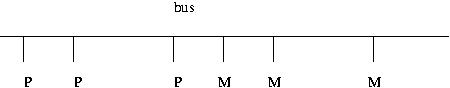
\includegraphics{Images/UMABus.jpg}

Here and below:

\begin{itemize}

\item The Ps are processors, e.g. off-the-shelf chips such as Pentiums.

\item The Ms are \textbf{memory modules}. These are physically separate
objects, e.g. separate boards of memory chips.  It is typical that there
will be the same number of Ms as Ps.

\item To make sure only one P uses the bus at a time, standard bus
arbitration signals and/or arbitration devices are used.

\item There may also be \textbf{coherent caches}, which we will discuss later.

\end{itemize}

\subsection{NUMA Systems}

In a {\bf Nonuniform Memory Access} (NUMA) architecture, each CPU has a
memory module physically next to it, and these processor/memory (P/M)
pairs are connected by some kind of network.

Here is a simple version:

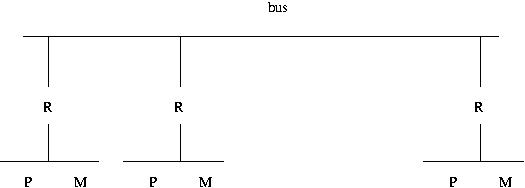
\includegraphics{Images/NUMABus.jpg}

Each P/M/R set here is called a \textbf{processing element} (PE). Note
that each PE has its own local bus, and is also connected to the global
bus via R, the router.

Suppose for example that P3 needs to access location 200, and suppose
that high-order interleaving is used.  If location 200 is in M3, then
P3's request is satisfied by the local bus.\footnote{This sounds similar
to the concept of a cache. However, it is very different.  A cache
contains a local copy of some data stored elsewhere.  Here it is the
data itself, not a copy, which is being stored locally.} On the other
hand, suppose location 200 is in M8. Then the R3 will notice this, and
put the request on the global bus, where it will be seen by R8, which
will then copy the request to the local bus at PE8, where the request
will be satisfied.  (E.g. if it was a read request, then the response
will go back from M8 to R8 to the global bus to R3 to P3.)

It should be obvious now where NUMA gets its name. P8 will have much
faster access to M8 than P3 will to M8, if none of the buses is
currently in use---and if say the global bus is currently in use, P3
will have to wait a long time to get what it wants from M8.

Today almost all high-end MIMD systems are NUMAs.  One of the attractive
features of NUMA is that by good programming we can exploit the
nonuniformity.  In matrix problems, for example, we can write our
program so that, for example, P8 usually works on those rows of the
matrix which are stored in M8, P3 usually works on those rows of the
matrix which are stored in M3, etc. In order to do this, we need to make
use of the C language's \& address operator, and have some knowledge of
the memory hardware structure, i.e. the interleaving.

\subsection{NUMA Interconnect Topologies}

The problem with a bus connection, of course, is that there is only one
pathway for communication, and thus only one processor can access memory
at the same time.  If one has more than, say, two dozen processors are
on the bus, the bus becomes saturated, even if traffic-reducing methods
such as adding caches are used. Thus multipathway topologies are used
for all but the smallest systems.  In this section we look at two
alternatives to a bus topology.

\subsubsection{Crossbar Interconnects}

Consider a shared-memory system with n processors and n memory modules.
Then a crossbar connection would provide \( n^{2} \) pathways. E.g. for n =
8:

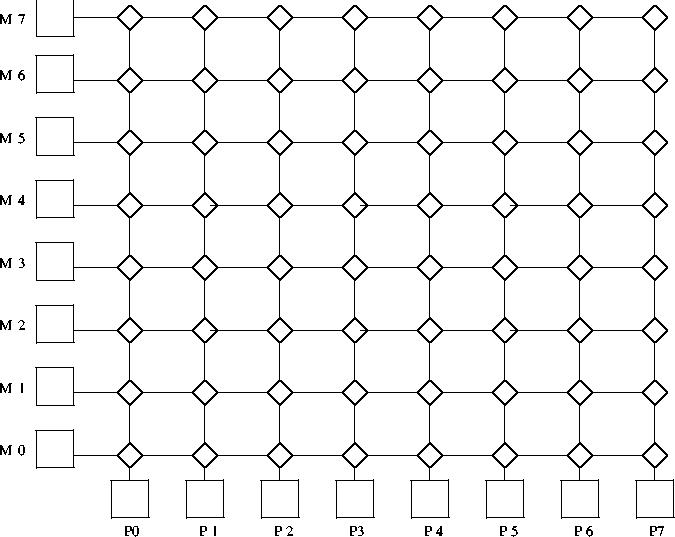
\includegraphics{Images/XBar.jpg}

Generally serial communication is used from node to node, with a packet
containing information on both source and destination address. E.g. if
P2 wants to read from M5, the source and destination will be 3-bit
strings in the packet, coded as 010 and 101, respectively.  The packet
will also contain bits which specify which word within the module we
wish to access, and bits which specify whether we wish to do a read or a
write.  In the latter case, additional bits are used to specify the
value to be written.

Each diamond-shaped node has two inputs (bottom and right) and two
outputs (left and top), with buffers at the two inputs.  If a buffer
fills, there are two design options: (a) Have the node from which the
input comes block at that output. (b) Have the node from which the input
comes discard the packet, and retry later, possibly outputting some
other packet for now.  If the packets at the heads of the two buffers
both need to go out the same output, the one (say) from the bottom input
will be given priority.

There could also be a return network of the same type, with this one
being memory \( \rightarrow  \) processor, to return the result of the
read requests.\footnote{For safety's sake, i.e. fault tolerance, even
writes are typically acknowledged in multiprocessor systems.}

Another version of this is also possible. It is not shown here, but the
difference would be that at the bottom edge we would have the PEi and at
the left edge the memory modules Mi would be replaced by lines which
wrap back around to PEi, similar to the Omega network shown below.

Crossbar switches are too expensive for large-scale systems, but are
useful in some small systems. The 16-CPU Sun Microsystems Enterprise
10000 system includes a 16x16 crossbar.

\subsubsection{Omega (or Delta) Interconnects}

These are multistage networks similar to crossbars, but with fewer
paths. Here is an example of a NUMA 8x8 system:

\par

\centerline{
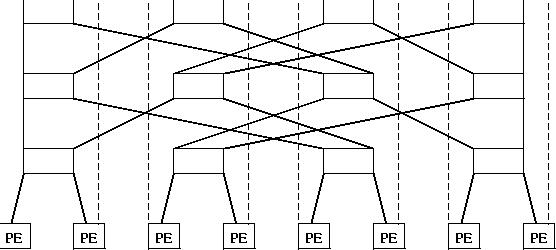
\includegraphics[height=1.0in]{Images/Omega.jpg}
}

Recall that each PE is a processor/memory pair.  PE3, for instance,
consists of P3 and M3.

Note the fact that at the third stage of the network (top of picture),
the outputs are routed back to the PEs, each of which consists of a
processor and a memory module.\footnote{The picture may be cut off somewhat
at the top and left edges.  The upper-right output of the rectangle in
the top row, leftmost position should connect to the dashed line which
leads down to the second PE from the left.  Similarly, the upper-left
output of that same rectangle is a dashed lined, possibly invisible in
your picture, leading down to the leftmost PE.}

At each network node (the nodes are the three rows of rectangles), the
output routing is done by destination bit. Let's number the stages here
0, 1 and 2, starting from the bottom stage, number the nodes within a
stage 0, 1, 2 and 3 from left to right, number the PEs from 0 to 7, left
to right, and number the bit positions in a destination address 0, 1 and
2, starting from the most significant bit. Then at stage i, bit i of the
destination address is used to determine routing, with a 0 meaning
routing out the left output, and 1 meaning the right one.

Say P2 wishes to read from M5. It sends a read-request packet, including
5 = 101 as its destination address, to the switch in stage 0, node 1.
Since the first bit of 101 is 1, that means that this switch will route
the packet out its right-hand output, sending it to the switch in stage
1, node 3. The latter switch will look at the next bit in 101, a 0, and
thus route the packet out its left output, to the switch in stage 2,
node 2. Finally, that switch will look at the last bit, a 1, and output
out its right-hand output, sending it to PE5, as desired. M5 will
process the read request, and send a packet back to PE2, along the same

Again, if two packets at a node want to go out the same output, one must
get priority (let's say it is the one from the left input).

Here is how the more general case of N = \( 2^{n} \) PEs works. Again
number the rows of switches, and switches within a row, as above. So, \(
S_{ij} \) will denote the switch in the i-th row from the bottom and
j-th column from the left (starting our numbering with 0 in both cases).
Row i will have a total of N input ports \( I_{ik} \) and N output ports
\( O_{ik} \), where k = 0 corresponds to the leftmost of the N in each
case. Then if row i is not the last row (\( i<n-1 \)), \( O_{ik} \) will
be connected to \( I_{jm} \), where j = i+1 and

\begin{equation}
m = (2k + \lfloor (2k)/N \rfloor ) ~ mod ~ N
\end{equation}

If row i is the last row, then \( O_{ik} \) will be connected to, PE k.


\subsection{Comparative Analysis}

In the world of parallel architectures, a key criterion for a proposed
feature is \textbf{scalability}, meaning how well the feature performs
as we go to larger and larger systems. Let n be the system size, either
the number of processors and memory modules, or the number of PEs. Then
we are interested in how fast the latency, bandwidth and cost grow with
n:

\begin{tabular}{|l|r|r|r|}
\hline
criterion &
 bus &
 Omega&
 crossbar \\
\hline
latency &
 O(1) &
 $\rm O( \log_2 n)$ &
 O(n) \\
\hline
bandwidth &
 O(1) &
 O(n) &
 O(n) \\
\hline
cost &
 O(1) &
 $\rm O(n \log_2 n)$ &
$\rm  O(n^2)$ \\
\hline
\end{tabular}

Let us see where these expressions come from, beginning with a bus: No
matter how large n is, the time to get from, say, a processor to a
memory module will be the same, thus O(1). Similarly, no matter how
large n is, only one communication can occur at a time, thus again
O(1).\footnote{ Note that the `1' in ``O(1)'' does not refer to the fact
that only one communication can occur at a time. If we had, for example,
a two-bus system, the bandwidth would still be O(1), since
multiplicative constants do not matter. What O(1) means, again, is that
as n grows, the bandwidth stays at a multiple of 1, i.e.  stays
constant.  }

Again, we are interested only in ``O( )'' measures, because we are only
interested in growth rates as the system size n grows. For instance, if
the system size doubles, the cost of a crossbar will quadruple; the \(
O(n^{2}) \) cost measure tells us this, with any multiplicative constant
being irrelevant.

For Omega networks, it is clear that \( log_{2}n \) network rows are
needed, hence the latency value given. Also, each row will have n/2
switches, so the number of network nodes will be O(n \( log_{2}n \)).
This figure then gives the cost (in terms of switches, the main expense
here). It also gives the bandwidth, since the maximum number of
simultaneous transmissions will occur when all switches are sending at
once.

Similar considerations hold for the crossbar case.

The crossbar's big advantage is that it is guaranteed that n packets can
be sent simultaneously, providing they are to distinct
destinations.

That is \underbar{not} true for Omega-networks. If for example, PE0
wants to send to PE3, and at the same time PE4 wishes to sent to PE2,
the two packets will clash at the leftmost node of stage 1, where the
packet from PE0 will get priority.

On the other hand, a crossbar is very expensive, and thus is dismissed
out of hand in most modern systems. Note, though, that an equally
troublesom aspect of crossbars is their high latency value; this is a
big drawback when the system is not heavily loaded.

The bottom line is that Omega-networks amount to a compromise between
buses and crossbars, and for this reason have become popular.

\subsection{Why Have Memory in Modules?}

In the shared-memory case, the Ms collectively form the entire
shared address space, but with the addresses being assigned to the Ms in
one of two ways:

\begin{itemize}

\item (a)

High-order interleaving. Here consecutive addresses are in the
\underbar{same} M (except at boundaries). For example, suppose for
simplicity that our memory consists of addresses 0 through 1023, and
that there are four Ms.  Then M0 would contain addresses 0-255, M1 would
have 256-511, M2 would have 512-767, and M3 would have 768-1023.

\item (b)

Low-order interleaving. Here consecutive addresses are in consecutive
M's (except when we get to the right end). In the example above, if we
used low-order interleaving, then address 0 would be in M0, 1 would be
in M1, 2 would be in M2, 3 would be in M3, 4 would be back in M0, 5 in
M1, and so on.

\end{itemize}

The idea is to have several modules busy at once, say in conjunction
with a {\bf split-transaction bus}.  Here, after a processor makes a
memory request, it relinquishes the bus, allowing others to use it while
the memory does the requested work.  Without splitting the memory into
modules, this wouldn't achieve parallelism.  The bus does need extra
lines to identify which processor made the request.

% \subsubsection{Dealing with Latency Problems}
%
% The hardware and software may also be designed to reduce latency. One
% approach to this is \textbf{latency hiding}, which consists of
% prefetching a word or words from a certain section of memory which is to
% be used soon. It is somewhat similar to the idea of delayed branch in
% RISC processors. Suppose for instance we have code like
%
% \begin{verbatim}
% LD R4,200
% ADD R5,R2
% ADD R5,R3
% SUB R4,R5
% \end{verbatim}
%
% (where the Ri are registers).  The hardware design may be such that
% there is a PF (prefetch) instruction, which is \textbf{nonblocking},
% meaning that subsequent instructions can execute while the PF is still
% pending (as long as the subsequent instructions do not depend on the
% result of the PF). Then we could rewrite the above code as
%
% \begin{verbatim}
% PF R4,200
% ADD R5,R2
% ADD R1,R2
% SUB R4,R5
% \end{verbatim}
%
% Hopefully the PF will be done by the time we get to the SUB instruction.
% If not, SUB will block for the remaining time, but even then we will
% have saved time.


% \subsubsection{Internode Synchronization on Shared-Memory Hardware}

\section{Synchronization Hardware}

Avoidance of race conditions, e.g. implementation of locks, plays such a
crucial role in shared-memory parallel processing that hardware
assistance is a virtual necessity.  Recall, for instance, that critical
sections can effectively serialize a parallel program.  Thus efficient
implementation is crucial.

\subsection{Test-and-Set Instructions}

Consider a bus-based system. In addition to whatever memory read and
memory write instructions the processor included, there would also be a
TAS instruction.\footnote{This discussion is for a mythical machine, but
any real system works in this manner.}  This instruction would control a
TAS pin on the processor chip, and the pin in turn would be connected to
a TAS line on the bus.

Applied to a location L in memory and a register R, say, TAS does the
following:

\begin{Verbatim}[fontsize=\relsize{-2}]
   copy L to R
   if R is 0 then write 1 to L
\end{Verbatim}

And most importantly, these operations are done in an \textbf{atomic}
manner; no bus transactions by other processors may occur between the
two steps.

The TAS operation is applied to variables used as locks. Let's say that
1 means locked and 0 unlocked. Then the guarding of a critical section C
by a lock variable L, using a register R, would be done by having the
following code in the program being run:

\begin{Verbatim}[fontsize=\relsize{-2}]
   TRY:  TAS R,L
         JNZ TRY
     C:  ...   ; start of critical section
         ...
         ...   ; end of critical section
         MOV 0,L  ; unlock
\end{Verbatim}

where of course JNZ is a jump-if-nonzero instruction, and we are
assuming that the copying from the Memory Data Register to R results in
the processor N and Z flags (condition codes) being affected.

\subsubsection{LOCK Prefix on Intel Processors}
\label{lockprefix}


On Pentium machines, the LOCK prefix can be used to get atomicity for
certain instructions:  ADD, ADC, AND, BTC, BTR, BTS, CMPXCHG, DEC, INC,
NEG, NOT, OR, SBB, SUB, XOR, XADD.  The bus will be locked for the
duration of the execution of the instruction, thus setting up atomic
operations.  There is a special LOCK line in the control bus for this
purpose.  (Locking thus only applies to these instructions in forms in
which there is an operand in memory.) By the way, XCHG asserts this
LOCK\# bus signal even if the LOCK prefix is not specified.

For example, consider our count-the-2s example on  page
\pageref{count2s}.  If we store {\bf mycount} in a register, say EDX,
then

\begin{lstlisting}
lock add %edx, overallcount
\end{lstlisting}

would replace the code we had earlier,

\begin{lstlisting}
pthread_mutex_lock(&nextbaselock);
overallcount += mylocalcount;
pthread_mutex_unlock(&nextbaselock);
\end{lstlisting}

without locks!

Here is how we could implement a lock if needed.  The lock would be in a
variable named, say, {\bf lockvar}.

\begin{lstlisting}
   movl $lockvar, %ebx
   movl $1, %ecx
top:
   movl $0, %eax
   lock cmpxchg (%ebx), %ecx
   jz top  # else leave the loop and enter the critical section
\end{lstlisting}

The operation CMPXCHG has EAX as an unnamed operand.  The instruction
basically does (here {\bf source} is ECX and {\bf destination} is {\bf
lockvar})

\begin{lstlisting}
if c(EAX) != c(destination)  # sorry, lock is already locked
   c(EAX) <- c(destination)
   ZF <- 0  # the Zero Flag in the EFLAGS register
else
   c(destination) <- c(source)  # lock the lock
   ZF <- 1
\end{lstlisting}

The LOCK prefix locks the bus for the entire duration of the
instruction.  Note that the ADD instruction here involves two memory
transactions---one to read the old value of {\bf overallcount}, and the
second the write the new, incremented value back to {\bf overallcount}.
So, we are locking for a rather long time, potentially compromising
performance when other threads want to access memory, but the benefits
can be huge.

\subsubsection{Locks with More Complex Interconnects}

In crossbar or $\Omega$-network systems, some 2-bit field in the packet
must be devoted to transaction type, say 00 for Read, 01 for Write and
10 for TAS.  In a sytem with 16 CPUs and 16 memory modules, say, the
packet might consist of 4 bits for the CPU number, 4 bits for the memory
module number, 2 bits for the transaction type, and 32 bits for the data
(for a write, this is the data to be written, while for a read, it would
be the requested value, on the trip back from the memory to the CPU).

But note that the atomicity here is best done at the memory, i.e. some
hardware should be added at the memory so that TAS can be done;
otherwise, an entire processor-to-memory path (e.g. the bus in a
bus-based system) would have to be locked up for a fairly long time,
obstructing even the packets which go to other memory modules.

\subsection{May Not Need the Latest}

Note carefully that in many settings it may not be crucial to get the
most up-to-date value of a variable.  For example, a program may have a
data structure showing work to be done.  Some processors occasionally
add work to the queue, and others take work from the queue.  Suppose the
queue is currently empty, and a processor adds a task to the queue, just
as another processor is checking the queue for work.  As will be seen
later, it is possible that even though the first processor has written
to the queue, the new value won't be visible to other processors for
some time.  But the point is that if the second processor does not see
work in the queue (even though the first processor has put it there),
the program will still work correctly, albeit with some performance
loss.

\subsection{Fetch-and-Add Instructions}
\label{fanda}

Another form of interprocessor synchronization is a
\textbf{fetch-and-add} (FA) instruction.  The idea of FA is as follows.
For the sake of simplicity, consider code like

\begin{Verbatim}[fontsize=\relsize{-2}]
LOCK(K);
Y = X++;
UNLOCK(K);
\end{Verbatim}

Suppose our architecture's instruction set included an F\&A instruction.
It would add 1 to the specified location in memory, and return the old
value (to {\bf Y}) that had been in that location before being incremented.
And all this would be an atomic operation.

We would then replace the code above by a library call, say,

\begin{Verbatim}[fontsize=\relsize{-2}]
FETCH_AND_ADD(X,1);
\end{Verbatim}

The C code above would compile to, say,

\begin{Verbatim}[fontsize=\relsize{-2}]
F&A X,R,1
\end{Verbatim}

where {\bf R} is the register into which the old (pre-incrementing)
value of {\bf X} would be returned.

There would be hardware adders placed at each memory module. That means
that the whole operation could be done in one round trip to memory.
Without F\&A, we would need two round trips to memory just for the

\begin{Verbatim}[fontsize=\relsize{-2}]
X++;
\end{Verbatim}

(we would load {\bf X} into a register in the CPU, increment the register, and
then write it back to {\bf X} in memory), and then the LOCK() and UNLOCK()
would need trips to memory too.  This could be a huge time savings,
especially for long-latency interconnects.

\section{Cache Issues}
\label{cacheissues}

If you need a review of cache memories or don't have background in that
area at all, read Section \ref{cache} in the appendix of this book
before continuing.

\subsection{Cache Coherency}
\label{cachecoherency}

Consider, for example, a bus-based system. Relying purely on TAS for
interprocessor synchronization would be unthinkable: As each processor
contending for a lock variable spins in the loop shown above, it is
adding tremendously to bus traffic.

An answer is to have caches at each processor.\footnote{The reader may
wish to review the basics of caches.  See for example
\url{http://heather.cs.ucdavis.edu/~matloff/50/PLN/CompOrganization.pdf}.}
These will store copies of the values of lock variables.  (Of course,
non-lock variables are stored too.  However, the discussion here will
focus on effects on lock variables.) The point is this: Why keep looking
at a lock variable L again and again, using up the bus bandwidth? L may
not change value for a while, so why not keep a copy in the cache,
avoiding use of the bus?

The answer of course is that eventually L \underbar{will} change value,
and this causes some delicate problems. Say for example that processor
P5 wishes to enter a critical section guarded by L, and that processor
P2 is already in there. During the time P2 is in the critical section,
P5 will spin around, always getting the same value for L (1) from C5,
P5's cache. When P2 leaves the critical section, P2 will set L to
0---and now C5's copy of L will be incorrect. This is the \textbf{cache
coherency problem}, inconsistency between caches.

A number of solutions have been devised for this problem. For bus-based
systems, \textbf{snoopy} protocols of various kinds are used, with the
word ``snoopy'' referring to the fact that all the caches monitor
(``snoop on'') the bus, watching for transactions made by
\underbar{other} caches.

The most common protocols are the \textbf{invalidate} and
\textbf{update} types.  This relation between these two is somewhat
analogous to the relation between \textbf{write-back} and
\textbf{write-through} protocols for caches in uniprocessor systems:

\begin{itemize}

\item Under an invalidate protocol, when a processor writes to a
variable in a cache, it first (i.e. before actually doing the write)
tells each other cache to mark as invalid its cache line (if any) which
contains a copy of the variable.\footnote{We will follow commonly-used
terminology here, distinguishing between a {\it cache line} and a {\it
memory block}.  Memory is divided in blocks, some of which have copies
in the cache.  The cells in the cache are called {\it cache lines}.  So,
at any given time, a given cache line is either empty or contains a copy
(valid or not) of some memory block.} Those caches will be updated only
later, the next time their processors need to access this cache line.

\item For an update protocol, the processor which writes to the variable
tells all other caches to immediately update their cache lines
containing copies of that variable with the new value.

\end{itemize}

Let's look at an outline of how one implementation (many variations exist)
of an invalidate protocol would operate:

In the scenario outlined above, when P2 leaves the critical section, it
will write the new value 0 to L. Under the invalidate protocol, P2 will
post an invalidation message on the bus. All the other caches will
notice, as they have been monitoring the bus. They then mark their
cached copies of the line containing L as invalid.

Now, the next time P5 executes the TAS instruction---which will be very
soon, since it is in the loop shown above---P5 will find that the copy
of L in C5 is invalid. It will respond to this cache miss by going to
the bus, and requesting P2 to supply the ``real'' (and valid) copy of
the line containing L.

But there's more.  Suppose that all this time P6 had also been executing
the loop shown above, along with P5.  Then P5 and P6 may have to contend
with each other.  Say P6 manages to grab possession of the bus
first.\footnote{Again, remember that ordinary bus arbitration methods
would be used.} P6 then executes the TAS again, which finds L = 0 and
changes L back to 1.  P6 then relinquishes the bus, and enters the
critical section.  Note that in changing L to 1, P6 also sends an
invalidate signal to all the other caches.  So, when P5 tries its
execution of the TAS again, it will have to ask P6 to send a valid copy
of the block.  P6 does so, but L will be 1, so P5 must resume executing
the loop. P5 will then continue to use its valid local copy of L each
time it does the TAS, until P6 leaves the critical section, writes 0 to
L, and causes another cache miss at P5, etc.

At first the update approach seems obviously superior, and actually, if
our shared, cacheable\footnote{ Many modern processors, including
Pentium and MIPS, allow the programmer to mark some blocks as being
noncacheable.} variables were only lock variables, this might be true.

But consider a shared, cacheable vector. Suppose the vector fits into
one block, and that we write to each vector element sequentially. Under
an update policy, we would have to send a new message on the bus/network
for each component, while under an invalidate policy, only one message
(for the first component) would be needed. If during this time the other
processors do not need to access this vector, all those update messages,
and the bus/network bandwidth they use, would be wasted.

Or suppose for example we have code like

\begin{Verbatim}[fontsize=\relsize{-2}]
Sum += X[I];
\end{Verbatim}

in the middle of a \textbf{for} loop. Under an update protocol, we would
have to write the value of Sum back many times, even though the other
processors may only be interested in the final value when the loop ends.
(This would be true, for instance, if the code above were part of a
critical section.)

Thus the invalidate protocol works well for some kinds of code, while
update works better for others.  The CPU designers must try to
anticipate which protocol will work well across a broad mix of
applications.\footnote{Some protocols change between the two modes
dynamically.}

Now, how is cache coherency handled in non-bus shared-memory systems,
say crossbars?  Here the problem is more complex. Think back to the bus
case for a minute: The very feature which was the biggest negative
feature of bus systems---the fact that there was only one path between
components made bandwidth very limited---is a very \underbar{positive}
feature in terms of cache coherency, because it makes
\underbar{broadcast} very easy: Since everyone is attached to that
single pathway, sending a message to all of them costs no more than
sending it to just one---we get the others for free. That's no longer
the case for multipath systems. In such systems, extra copies of the
message must be created for each path, adding to overall traffic.

A solution is to send messages only to ``interested parties.'' In
\textbf{directory-based} protocols, a list is kept of all caches
which currently have valid copies of all blocks. In one common
implementation, for example, while P2 is in the critical section above,
it would be the \textbf{owner} of the block containing L. (Whoever is
the latest node to write to L would be considered its current owner.) It
would maintain a directory of all caches having valid copies of that
block, say C5 and C6 in our story here. As soon as P2 wrote to L, it
would then send either invalidate or update packets (depending on which
type was being used) to C5 and C6 (and \underbar{not} to other caches
which didn't have valid copies).

There would also be a directory at the memory, listing the current
owners of all blocks. Say for example P0 now wishes to ``join the
club,'' i.e. tries to access L, but does not have a copy of that block
in its cache C0.  C0 will thus not be listed in the directory for this
block.  So, now when  it tries to access L and it will get a cache miss.
P0 must now consult the {\bf home} of L, say P14.  The home might be
determined by L's location in main memory according to high-order
interleaving; it is the place where the main-memory version of L
resides.  A table at P14 will inform P0 that P2 is the current owner of
that block. P0 will then send a message to P2 to add C0 to the list of
caches having valid copies of that block.  Similarly, a cache might
``resign'' from the club, due to that cache line being replaced, e.g. in
a LRU setting, when some other cache miss occurs.

\subsection{Example: the MESI Cache Coherency Protocol}

Many types of cache coherency protocols have been proposed and used,
some of them quite complex. A relatively simple one for snoopy bus
systems which is widely used is MESI, which for example is the protocol
used in the Pentium series.

MESI is an invalidate protocol for bus-based systems.  Its name stands
for the four states a given cache line can be in for a given CPU:

\begin{itemize}

\item Modified
\item Exclusive
\item Shared
\item Invalid

\end{itemize}

Note that {\it each memory block} has such a state at {\it each cache}.
For instance, block 88 may be in state S at P5's and P12's caches but in
state I at P1's cache.

Here is a summary of the meanings of the states:


\begin{tabular}{|c|c|}
\hline
state&
 meaning\\
\hline
M&
 written to more than once; no other copy valid\\
\hline
E&
 valid; no other cache copy valid; memory copy valid\\
\hline
S&
 valid; at least one other cache copy valid\\
\hline
I&
 invalid (block either not in the cache or present but incorrect) \\
\hline
\end{tabular}

\par{} \vspace{0.3cm}

Following is a summary of MESI state changes.\footnote{See \emph{Pentium
Processor System Architecture}, by D. Anderson and T.  Shanley,
Addison-Wesley, 1995. We have simplified the presentation here, by
eliminating certain programmable options.} When reading it, keep in mind
again that there is a separate state for each cache/memory block combination.

In addition to the terms \textbf{read hit}, \textbf{read miss},
\textbf{write} \textbf{hit}, \textbf{write miss}, which you are already
familiar with, there are also \textbf{read snoop} and \textbf{write
snoop}.  These refer to the case in which our CPU observes on the bus a
block request by another CPU that has attempted a read or write action
but encountered a miss in its own cache; if our cache has a valid copy
of that block, we must provide it to the requesting CPU (and in some
cases to memory).

So, here are various events and their corresponding state changes:

{\bf If our CPU does a read:}

\begin{tabular}{|c|c|c|}
\hline
present state&
 event&
 new state\\
\hline
M&
 read hit&
 M\\
\hline
E&
 read hit&
 E\\
\hline
S&
 read hit&
 S\\
\hline
I&
 read miss; no valid cache copy at any other CPU &
 E\\
\hline
I&
 read miss; at least one valid cache copy in some other CPU &
 S  \\
\hline
\end{tabular}

\par{} \vspace{0.3cm}

{\bf If our CPU does a memory write:}

\begin{tabular}{|c|c|c|}
\hline
present state&
 event&
 new state\\
\hline
M&
 write hit; do not put invalidate signal on bus; do not update memory&
 M\\
\hline
E&
 same as M above&
 M\\
\hline
S&
 write hit; put invalidate signal on bus; update memory&
 E\\
\hline
I&
 write miss; update memory but do nothing else&
 I  \\
\hline
\end{tabular}

\par{} \vspace{0.3cm}

{\bf If our CPU does a read or write snoop:}

\begin{tabular}{|c|c|c|}
\hline
present state&
 event&
 newstate\\
\hline
M&
 read snoop; write line back to memory, picked up by other CPU&
 S\\
\hline
M&
 write snoop; write line back to memory, signal other CPU now OK to do its
 write&
 I\\
\hline
E&
 read snoop; put shared signal on bus; no memory action&
 S\\
\hline
E&
 write snoop; no memory action&
 I\\
\hline
S&
 read snoop&
 S\\
\hline
S&
 write snoop&
 I\\
\hline
I&
 any snoop&
 I \\
\hline
\end{tabular}

Note that a write miss does NOT result in the associated block being
brought in from memory.

Example:  Suppose a given memory block has state M at processor A but
has state I at processor B, and B attempts to write to the block.  B
will see that its copy of the block is invalid, so it notifies the other
CPUs via the bus that it intends to do this write.  CPU A sees this
announcement, tells B to wait, writes its own copy of the block
back to memory, and then tells B to go ahead with its write.  The
latter action means that A's copy of the block is not correct anymore,
so the block now has state I at A.  B's action does not cause loading of
that block from memory to its cache, so the block still has state I at
B.

\par{} \vspace{0.3cm}

\subsection{The Problem of ``False Sharing''}

Consider the C declaration

\begin{Verbatim}[fontsize=\relsize{-2}]
int W,Z;
\end{Verbatim}

Since {\bf W} and {\bf Z} are declared adjacently, most compilers will
assign them contiguous memory addresses.  Thus, unless one of them is at
a memory block boundary, when they are cached they will be stored in the
same cache line.  Suppose the program writes to {\bf Z}, and our system
uses an invalidate protocol.  Then {\bf W} will be considered invalid at
the other processors, even though its values at those processors' caches
are correct.  This is the {\bf false sharing} problem, alluding to the
fact that the two variables are sharing a cache line even though they
are not related.

This can have very adverse impacts on performance.  If for instance our
variable {\bf W} is now written to, then {\bf Z} will suffer unfairly,
as its copy in the cache will be considered invalid even though it is
perfectly valid.  This can lead to a ``ping-pong'' effect, in which
alternate writing to two variables leads to a cyclic pattern of
coherency transactions.

One possible solution is to add padding, e.g. declaring {\bf W} and {\bf
Z} like this:

\begin{Verbatim}[fontsize=\relsize{-2}]
int W,U[1000],Z;
\end{Verbatim}

to separate {\bf W} and {\bf Z} so that they won't be in the same cache
block.  Of course, we must take block size into account, and check
whether the compiler really has placed the two variables are in widely
separated locations.  To do this, we could for instance run the code

\begin{Verbatim}[fontsize=\relsize{-2}]
printf("%x %x\n,&W,&Z);
\end{Verbatim}

\section{Memory-Access Consistency Policies}
\label{consistency}

Though the word {\it consistency} in the title of this section may seem
to simply be a synonym for {\it coherency} from the last section, and
though there actually is some relation, the issues here are quite
different.  In this case, it is a timing issue:  After one processor
changes the value of a shared variable, when will that value be
visible to the other processors?

There are various reasons why this is an issue.  For example, many
processors, especially in multiprocessor systems, have {\bf write
buffers}, which save up writes for some time before actually sending
them to memory.  (For the time being, let's suppose there are no
caches.) The goal is to reduce memory access costs.  Sending data to
memory in groups is generally faster than sending one at a time, as the
overhead of, for instance, acquiring the bus is amortized over many
accesses.  Reads following a write may proceed, without waiting for the
write to get to memory, except for reads to the same address.  So in a
multiprocessor system in which the processors use write buffers, there
will often be some delay before a write actually shows up in memory.

A related issue is that operations may occur, or appear to occur, out of
order.  As noted above, a read which follows a write in the program may
execute before the write is sent to memory.  Also, in a multiprocessor
system with multiple paths between processors and memory modules, two
writes might take different paths, one longer than the other, and arrive
``out of order.''  In order to simplify the presentation here, we will
focus on the case in which the problem is due to write buffers, though.

The designer of a multiprocessor system must adopt some {\bf consistency
model} regarding situations like this.  The above discussion shows that
the programmer must be made aware of the model, or risk getting
incorrect results.  Note also that different consistency models will
give different levels of performance.  The ``weaker'' consistency models
make for faster machines but require the programmer to do more work.

The strongest consistency model is Sequential Consistency.  It
essentially requires that memory operations done by one processor
are observed by the other processors to occur in the same order as
executed on the first processor.  Enforcement of this requirement makes
a system slow, and it has been replaced on most systems by weaker
models.

One such model is {\bf release consistency}.  Here the processors' instruction
sets include instructions ACQUIRE and RELEASE.  Execution of an ACQUIRE
instruction at one processor involves telling all other processors to
flush their write buffers.  However, the ACQUIRE won't execute until
pending RELEASEs are done.  Execution of a RELEASE basically means that
you are saying, "I'm done writing for the moment, and wish to allow
other processors to see what I've written."  An ACQUIRE waits for all
pending RELEASEs to complete before it executes.\footnote{There are many
variants of all of this, especially in the software distibuted shared
memory realm, to be discussed later.}

A related model is {\bf scope consistency}.  Say a variable, say {\bf
Sum}, is written to within a critical section guarded by LOCK and UNLOCK
instructions.  Then under scope consistency any changes made by one
processor to {\bf Sum} within this critical section would then be
visible to another processor when the latter next enters this critical
section.  The point is that memory update is postponed until it is
actually needed.  Also, a barrier operation (again, executed at the
hardware level) forces all pending memory writes to complete.

All modern processors include instructions which implement consistency
operations.  For example, Sun Microsystems' SPARC has a MEMBAR
instruction.  If used with a STORE operand, then all pending writes at
this processor will be sent to memory.  If used with the LOAD operand,
all writes will be made visible to this processor.

Now, how does cache coherency fit into all this?  There are many
different setups, but for example let's consider a design in which there
is a write buffer between each processor and its cache.  As the
processor does more and more writes, the processor saves them up in the
write buffer.  Eventually, some programmer-induced event, e.g. a MEMBAR
instruction,\footnote{We call this ``programmer-induced,'' since the
programmer will include some special operation in her C/C++ code which
will be translated to MEMBAR.} will cause the buffer to be flushed.
Then the writes will be sent to ``memory''---actually meaning that they
go to the cache, and then possibly to memory.

The point is that (in this type of setup) before that flush of the write
buffer occurs, the cache coherency system is quite unaware of these
writes.  Thus the cache coherency operations, e.g. the various actions
in the MESI protocol, won't occur until the flush happens.

To make this notion concrete, again consider the example with {\bf Sum}
above, and assume release or scope consistency.  The CPU currently
executing that code (say CPU 5) writes to {\bf Sum}, which is
a memory operation---it affects the cache and thus eventually the main
memory---but that operation will be invisible to the cache coherency
protocol for now, as it will only be reflected in this processor's write
buffer.  But when the unlock is finally done (or a barrier is reached),
the write buffer is flushed and the writes are sent to this CPU's cache.
That then triggers the cache coherency operation (depending on the
state).  The point is that the cache coherency operation would occur
only now, not before.

What about reads?  Suppose another processor, say CPU 8, does a read of
{\bf Sum}, and that page is marked invalid at that processor.  A cache
coherency operation will then occur.  Again, it will depend on the type
of coherency policy and the current state, but in typical systems this
would result in {\bf Sum}'s cache block being shipped to CPU 8 from
whichever processor the cache coherency system thinks has a valid copy
of the block.  That processor may or may not be CPU 5, but even if it
is, that block won't show the recent change made by CPU 5 to {\bf Sum}.

The analysis above assumed that there is a write buffer between each
processor and its cache.  There would be a similar analysis if there
were a write buffer between each cache and memory.

Note once again the performance issues.  Instructions such as ACQUIRE or
MEMBAR will use a substantial amount of interprocessor communication
bandwidth.  A consistency model must be chosen carefully by the system
designer, and the programmer must keep the communication costs in mind
in developing the software.

The recent Pentium models use Sequential Consistency, with any write
done by a processor being immediately sent to its cache as well.

\section{Fetch-and-Add Combining within Interconnects}

In addition to read and write operations being specifiable in a network
packet, an F\&A operation could be specified as well (a 2-bit field in
the packet would code which operation was desired). Again, there would
be adders included at the memory modules, i.e. the addition would be
done at the memory end, not at the processors. When the F\&A packet
arrived at a memory module, our variable  {\bf X} would have 1 added to
it, while the old value would be sent back in the return packet (and put
into R).

Another possibility for speedup occurs if our system uses a multistage
interconnection network such as a crossbar.  In that situation, we can
design some intelligence into the network nodes to do {\bf packet
combining}: Say more than one CPU is executing an F\&A operation at
about the same time for the same variable {\bf X}.  Then more than one
of the corresponding packets may arrive at the same network node at
about the same time.  If each one requested an incrementing of {\bf X}
by 1, the node can replace the two packets by one, with an increment of
2.  Of course, this is a delicate operation, and we must make sure that
different CPUs get different return values, etc.

\section{Multicore Chips}

A recent trend has been to put several CPUs on one chip, termed a {\bf
multicore} chip.  As of March 2008, dual-core chips are common in
personal computers, and quad-core machines are within reach of the
budgets of many people.  Just as the invention of the integrated circuit
revolutionized the computer industry by making computers affordable for
the average person, multicore chips will undoubtedly revolutionize the
world of parallel programming.

A typical dual-core setup might have the two CPUs sharing a common L2
cache, with each CPU having its own L1 cache.  The chip may interface to
the bus or interconnect network of via an L3 cache.

Multicore is extremely important these days.  However, they are just
SMPs, for the most part, and thus should not be treated differently.

\section{Optimal Number of Threads}

A common question involves the best number of threads to run in a
shared-memory setting.  Clearly there is no general magic answer, but
here are some considerations:\footnote{As with many aspects of parallel
programming, a good basic knowledge of operating systems is key.  See
the reference on page \pageref{needknowos}.}

\begin{itemize}

\item If your application does a lot of I/O, CPUs or cores may stay idle
while waiting for I/O events.  It thus makes sense to have many threads,
so that computation threads can run when the I/O threads are tied up.

\item In a purely computational application, one generally should not
have more threads than cores.  However, a program with a lot of virtual
memory page faults may benefit from setting up extra threads, as page
replacement involves (disk) I/O.

\item Applications in which there is heavy interthread communication,
say due to having a lot of lock variable, access, may benefit from
setting up fewer threads than the number of cores.

\item Many Intel processors include hardware for {\it hypertheading}.
These are not full threads in the sense of having separate cores, but
rather involve a limited amount of resource duplication within a core.
The performance gain from this is typically quite modest.  In any case,
be aware of it; some software systems count these as threads, and assume
for instance that there are 8 cores when the machine is actually just
quad core.

\item With GPUs (Chapter \ref{chap:cuda}), most memory accesses have
long latency and thus are I/O-like.  Typically one needs very large
numbers of threads for good performance.

\end{itemize}

\section{Processor Affinity}

With a timesharing OS, a given thread may run on different cores during
different timeslices.  If so, the cache for a given core may need a lot
of refreshing, each time a new thread runs on that core.  To avoid this
slowdown, one might designate a preferred core for each thread, in the
hope of reusing cache contents.  Setting this up is dependent on the
chip and the OS.  OpenMP 3.1 has some facility for this.

\section{Illusion of Shared-Memory through Software}
\label{sdsm}

\subsubsection{Software Distributed Shared Memory}

There are also various shared-memory software packages that run on
message-passing hardware such as NOWs, called \textbf{software
distributed shared memory} (SDSM) systems.  Since the platforms do not
have any physically shared memory, the shared-memory view which the
programmer has is just an illusion.  But that illusion is very useful,
since the shared-memory paradigm is believed to be the easier one to
program in.  Thus SDSM allows us to have ``the best of both
worlds''---the convenience of the shared-memory world view with the
inexpensive cost of some of the message-passing hardware systems,
particularly networks of workstations (NOWs).

SDSM itself is divided into two main approaches, the {\bf page-based}
and {\bf object-based} varieties.  The page-based approach is generally
considered clearer and easier to program in, and provides the programmer
the ``look and feel'' of shared-memory programming better than does the
object-based type.\footnote{The term {\it object-based} is not related
to the term {\it object-oriented programming}.}  We will discuss only
the page-based approach here.  The most popular SDSM system today is the
page-based Treadmarks (Rice University).  Another excellent page-based
system is JIAJIA (Academy of Sciences, China).

To illustrate how page-based SDSMs work, consider the line of JIAJIA code

\begin{Verbatim}[fontsize=\relsize{-2}]
Prime = (int *) jia_alloc(N*sizeof(int));
\end{Verbatim}

The function {\bf jia\_alloc()} is part of the JIAJIA library, {\bf
libjia.a}, which is linked to one's application program during
compilation.

At first this looks a little like a call to the standard {\bf malloc()}
function, setting up an array {\bf Prime} of size {\bf N}.  In fact, it
does indeed allocate some memory.  Note that each node in our JIAJIA
group is executing this statement, so each node allocates some memory at
that node.  Behind the scenes, not visible to the programmer, each node
will then have its own copy of {\bf Prime}.

However, JIAJIA sets things up so that when one node later accesses this
memory, for instance in the statement

\begin{Verbatim}[fontsize=\relsize{-2}]
Prime[I] = 1;
\end{Verbatim}

this action will eventually trigger a network transaction (not visible
to the programmer) to the other JIAJIA nodes.\footnote{There are a
number of important issues involved with this word {\it eventually}, as
we will see later.} This transaction will then update the copies of {\bf
Prime} at the other nodes.\footnote{The update may not occur
immediately.  More on this later.}

How is all of this accomplished?  It turns out that it relies on a
clever usage of the nodes' virtual memory (VM) systems.  To understand
this, you need a basic knowledge of how VM systems work.  If you lack
this, or need review, read Section \ref{vm} in the appendix of this book
before continuing.

Here is how VM is exploited to develop SDSMs on Unix systems.  The
SDSM will call a system function such as {\bf mprotect()}.  This allows
the SDSM to deliberately mark a page as nonresident (even if the
page {\it is} resident).  Basically, anytime the SDSM knows that a
node's local copy of a variable is invalid, it will mark the page
containing that variable as nonresident.  Then, the next time the
program at this node tries to access that variable, a page fault will
occur.

As mentioned in the review above, normally a page fault causes a jump to
the OS.  However, technically any page fault in Unix is handled as a
signal, specifically SIGSEGV.  Recall that Unix allows the programmer to
write his/her own signal handler for any signal type.  In this case,
that means that the programmer---meaning the people who developed JIAJIA
or any other page-based SDSM---writes his/her own page fault handler,
which will do the necessary network transactions to obtain the latest
valid value for {\bf X}.

Note that although SDSMs are able to create an illusion of almost all
aspects of shared memory, it really is not possible to create the
illusion of shared pointer variables.  For example on shared memory
hardware we might have a variable like {\bf P}:

\begin{Verbatim}[fontsize=\relsize{-2}]
int Y,*P;
...
...
P = &Y;
...
\end{Verbatim}

There is no simple way to have a variable like {\bf P} in an SDSM.
This is because a pointer is an address, and each node in an SDSM
has its own memory separate address space.  The problem is that even
though the underlying SDSM system will keep the various copies of {\bf Y}
at the different nodes consistent with each other, {\bf Y} will be at a
potentially different address on each node.

All SDSM systems must deal with a software analog of the cache coherency
problem.  Whenever one node modifies the value of a shared variable,
that node must notify the other nodes that a change has been made.  The
designer of the system must choose between update or invalidate
protocols, just as in the hardware case.\footnote{Note, though, that we
are not actually dealing with a cache here.  Each node in the SDSM
system will have a cache, of course, but a node's cache simply stores
parts of that node's set of pages.  The coherency across nodes is across
pages, not caches.  We must insure that a change made to a given page is
eventually propropagated to pages on other nodes which correspond to
this one.} Recall that in non-bus-based shared-memory multiprocessors,
one needs to maintain a directory which indicates at which processor a
valid copy of a shared variable exists.  Again, SDSMs must take an
approach similar to this.

Similarly, each SDSM system must decide between sequential
consistency, release consistency etc.  More on this later.

Note that in the NOW context the internode communication at the SDSM
level is typically done by TCP/IP network actions.  Treadmarks uses UDP,
which is faster than TCP. but still part of the slow TCP/IP protocol
suite.  TCP/IP was simply not designed for this kind of work.
Accordingly, there have been many efforts to use more efficient network
hardware and software.  The most popular of these is the Virtual
Interface Architecture (VIA).

Not only are coherency actions more expensive in the NOW SDSM case than in
the shared-memory hardware case due to network slowness, there is also
expense due to granularity.  In the hardware case we are dealing with
cache blocks, with a typical size being 512 bytes.  In the SDSM case, we
are dealing with pages, with a typical size being 4096 bytes.  The
overhead for a cache coherency transaction can thus be large.

\subsubsection{Case Study:  JIAJIA}

\textbf{Programmer Interface}

We will not go into detail on JIAJIA programming here.  There is
a short tutorial on JIAJIA at
\url{http://heather.cs.ucdavis.edu/~matloff/jiajia.html}, but
here is an overview:

\begin{itemize}

\item One writes in C/C++ (or FORTRAN), making calls to the
JIAJIA library, which is linked in upon compilation.

\item The library calls include standard shared-memory operations for
lock, unlock, barrier, processor number, etc., plus some calls aimed
at improving performance.

\end{itemize}

Following is a JIAJIA example program, performing Odd/Even Transposition
Sort.  This is a variant on Bubble Sort, sometimes useful in parallel
processing contexts.\footnote{Though, as mentioned in the comments, it
is aimed more at message-passing contexts.}  The algorithm consists of n
phases, in which each processor alternates between trading with its left
and right neighbors.

\begin{Verbatim}[fontsize=\relsize{-2},numbers=left]
// JIAJIA example program:  Odd-Even Tranposition Sort

// array is of size n, and we use n processors; this would be more
// efficient in a "chunked" versions, of course (and more suited for a
// message-passing context anyway)

#include <stdio.h>
#include <stdlib.h>
#include <jia.h>  // required include; also must link via -ljia

// pointer to shared variable
float *x;  // array to be sorted

int n,  // range to check for primeness
    debug;  // 1 for debugging, 0 else


// does sort of m-element array y
void oddeven(float *y, int m)
{  int i,left=jiapid-1,right=jiapid+1;
   float newval;
   for (i=0; i < m; i++)  {
      if ((i+jiapid)%2 == 0)  {
         if (right < m)
            if (y[jiapid] > y[right]) newval = y[right];
      }
      else  {
         if (left >= 0)
            if (y[jiapid] < y[left]) newval = y[left];
      }
      jia_barrier();
      if ((i+jiapid)%2 == 0 && right < m || (i+jiapid)%2 == 1 && left >= 0)
            y[jiapid] = newval;
      jia_barrier();
   }
}

main(int argc, char **argv)
{  int i,mywait=0;
   jia_init(argc,argv);  // required init call
   // get command-line arguments (shifted for nodes > 0)
   if (jiapid == 0)  {
      n = atoi(argv[1]);
      debug = atoi(argv[2]);
   }
   else  {
      n = atoi(argv[2]);
      debug = atoi(argv[3]);
   }
   jia_barrier();
   // create a shared array x of length n
   x = (float *) jia_alloc(n*sizeof(float));
   // barrier recommended after allocation
   jia_barrier();
   // node 0 gets simple test array from command-line
   if (jiapid == 0)  {
      for (i = 0; i < n; i++)
         x[i] = atoi(argv[i+3]);
   }
   jia_barrier();
   if (debug && jiapid == 0)
      while (mywait == 0)  { ; }
   jia_barrier();
   oddeven(x,n);
   if (jiapid == 0)  {
      printf("\nfinal array\n");
      for (i = 0; i < n; i++)
         printf("%f\n",x[i]);
   }
   jia_exit();
}
\end{Verbatim}

\textbf{System Workings}

JIAJIA's main characteristics as an SDSM are:

\begin{itemize}

\item page-based

\item scope consistency

\item home-based

\item multiple writers

\end{itemize}

Let's take a look at these.

As mentioned earlier, one first calls {\bf jia\_alloc()} to set up one's
shared variables.  Note that this will occur at each node, so there are
multiple copies of each variable; the JIAJIA system ensures that these
copies are consistent with each other, though of course subject to the
laxity afforded by scope consistency.

Recall that under scope consistency, a change made to a shared variable
at one processor is guaranteed to be made visible to another processor
if the first processor made the change between lock/unlock operations
and the second processor accesses that variable between lock/unlock
operations on that same lock.\footnote{Writes will also be propagated at
barrier operations, but two successive arrivals by a processor to a
barrier can be considered to be a lock/unlock pair, by considering a
departure from a barrier to be a ``lock,'' and considering reaching a
barrier to be an ``unlock.'' So, we'll usually not mention barriers
separately from locks in the remainder of this subsection.}

Each page---and thus each shared variable---has a {\bf home} processor.
If another processor writes to a page, then later when it reaches the
unlock operation it must send all changes it made to the page back to
the home node.  In other words, the second processor calls {\bf
jia\_unlock()}, which sends the changes to its sister invocation of {\bf
jia\_unlock()} at the home processor.\footnote{The set of changes is
called a {\bf diff}, remiscent of the Unix file-compare command.  A
copy, called a {\bf twin}, had been made of the original page, which now
will be used to produce the diff.  This has substantial overhead.  The
Treadmarks people found that it took 167 microseconds to make a twin,
and as much as 686 microseconds to make a diff.} Say later a third
processor calls {\bf jia\_lock()} on that same lock, and then attempts
to read a variable in that page.  A page fault will occur at that
processor, resulting in the JIAJIA system running, which will then
obtain that page from the first processor.

Note that all this means the JIAJIA system at each processor must
maintain a page table, listing where each home page resides.\footnote{In
JIAJIA, that location is normally fixed, but JIAJIA does include
advanced programmer options which allow the location to migrate.}  At
each processor, each page has one of three states:  Invalid, Read-Only,
Read-Write.  State changes, though, are reported when lock/unlock
operations occur.  For example, if CPU 5 writes to a given page which
had been in Read-Write state at CPU 8, the latter will not hear about
CPU 5's action until some CPU does a lock.  This CPU need not be
CPI 8.  When one CPU does a lock, it must coordinate with all other
nodes, at which time state-change messages will be piggybacked onto
lock-coordination messages.

Note also that JIAJIA allows the programmer to specify which node should
serve as the home of a variable, via one of several forms of the {\bf
jia\_alloc()} call.  The programmer can then tailor his/her code
accordingly.  For example, in a matrix problem, the programmer may
arrange for certain rows to be stored at a given node, and then write
the code so that most writes to those rows are done by that processor.

The general principle here is that writes performed at one node can be
made visible at other nodes on a ``need to know'' basis.  If for
instance in the above example with CPUs 5 and 8, CPU 2 does not access
this page, it would be wasteful to send the writes to CPU 2, or for that
matter to even inform CPU 2 that the page had been written to.  This is
basically the idea of all non-Sequential consistency protocols, even
though they differ in approach and in performance for a given
application.

JIAJIA allows multiple writers of a page.  Suppose CPU 4 and CPU 15 are
simultaneously writing to a particular page, and the programmer has
relied on a subsequent barrier to make those writes visible to other
processors.\footnote{The only other option would be to use lock/unlock,
but then their writing would not be simultaneous.}  When the barrier is
reached, each will be informed of the writes of the other.\footnote{If
they are writing to the same variable, not just the same page, the
programmer would use locks instead of a barrier, and the situation would
not arise.}  Allowing multiple writers helps to reduce the performance
penalty due to false sharing.

% Say Node 3 is the first one to execute
%
% \begin{verbatim}
%
% X = 21;
%
% \end{verbatim}
%
% Since the page in which X lies will have no-access status, the attempted
% write to X by the application program at this node will cause a page
% fault at this node, detected by the hardware.  This causes an internal
% interrupt, so control is tranferred to the OS, which sends a SIGSEGV
% signal to the program.  Ordinary programs don't have signal handlers for
% page faults, but in our case SDSM makes key use of one.  Its SIGSEGV
% signal handler routine will call mprotect() again, this time setting
% permission for the program to access that page, and then will allow the
% program to write 21 to its local copy of x.\footnote{That will be in the
% region set up by malloc().}
%
% Let's suppse here for concreteness that the SDSM uses an update policy.
% Then it will send the value 21 (and in fact the entire page) to the
% other nodes.
%
% Say later Node 8 tries to execute something like
%
% \begin{verbatim}
%
% x = 4;
%
% \end{verbatim}
%
% Again, a page fault will occur, this time at Node 8.  The SDSM system at
% that node will then send this latest value of X to the other nodes.

% \subsubsection{Programming Around Consistency Issues}
% \label{workaround}
%
% Recall from Section \ref{consistency} that one when node in a
% shared-memory multiprocessor or SDSM changes the value of a shared
% variable, there may be some delay before the other nodes are aware of
% this new value.  The nature of the delay will be determined by the
% consistency policy implemented in the hardware or SDSM.
%
% The situation for SDSMs is the same.  The designers of an SDSM must also
% set a consistency policy.  For example, look at the JIAJIA example in
% Section \ref{sdsm}.  Consider the code
%
% \begin{Verbatim}[fontsize=\relsize{-2}]
% jia_lock(NEXTI_LOCK);
% NI = (*NextI)++;
% jia_unlock(NEXTI_LOCK);
% \end{Verbatim}
%
% JIAJIA is set up so that if a shared variable, in this case {\bf
% NextI},\footnote{Of course, technically the shared value is in {\bf
% *NextI}, not in {\bf NextI}.} is changed at one node, the {\bf
% jia\_unlock()} operation will trigger update messages to the other
% nodes, which will receive them when they subsequently execute {\bf
% jia\_lock()}.\footnote{The same lock, in this case {\bf NEXTI\_LOCK},
% must be used.}  Also, each execution of {\bf jia\_barrier()} will send to
% all nodes all changes made to all variables since the last execution of
% that function.\footnote{Note that this is time-consuming, and if one
% needs the barrier operation without performing such updates, JIAJIA
% offers the {\bf jia\_wait()} function.}  The programmer has some control
% over how much delay there will be; use of a barrier to induce updates
% may result in long delays, but on the other hand use of locks has its
% own delays, due to internode negotiation operations which must take
% place when {\bf jia\_lock()} is called.
%
% In other words, whether using shared-memory hardware or SDSMs, there
% will always be some delay before a change to a shared variable at one
% node is reflected at the other nodes.  Indeed, no matter what, it would
% be physically impossible for a node to be guaranteed that it has the
% absolute latest value of a variable.
%
% This is not a problem once one recognizes the situation and programs
% around it.  Since locks are key to this, it is most important to
% understand that locks do work.
%
% Consider a bus-based shared-memory multiprocessor, for instance.  Say
% processors 5 and 6 both have a lock variable {\bf L} in their cache,
% with value 0, i.e. unlocked, and that both processors happen to execute
% a TAS at roughly the same time.  Suppose the cache coherency protocol
% uses an invalidate policy.  Recall that a processor must notify the
% other processors of a pending write {\it before} it actually does the
% write.  Both processors 5 and 6 will attempt to do this, but one of them
% will acquire the bus first, freezing the other out.  Let's say this is
% processor 6.  That means that processor 5 will receive a notification
% that its value of {\bf L} is invalid, and that processor will then
% cancel the TAS it had been attempting to execute.  So, TAS
% \underline{is} working; there is no danger that both processors 5 and 6
% will acquire the lock here.
%
% Similarly, consider the situation in which the caches in processors 5
% and 6 show that {\bf L} is 1, i.e. locked, and processor 1 changes {\bf
% L} to 0.  There will be a delay before news of the change reaches
% processors 5 and 6, and it may be the case that execution of the TAS
% will result in the value 1, which is ``old.''  But there is no harm
% there; the only thing that happens is that one of them acquires the lock
% a little bit later than it might.
%
% Designers of shared-memory hardware must be extremely careful in setting
% up their cache coherency system and consistency policy in such a way
% that ensures that instructions like TAS will do the right thing in all
% possible scenarios.  Again, ``the right thing'' means that, for
% instance, two processors cannot both acquire a lock at the same time,
% even if it does mean some delay.
%
% Similarly, designers of SDSMs must take the some kind of care.  It is a
% little easier here than in the hardware case, since programmers are
% forced to ``consult'' with the SDSM system in attempting to acquire a
% lock.  For JIAJIA, for instance, the programmer must call {\bf
% jia\_lock()}, forcing a transfer of control to the JIAJIA library code.
% That code will then negotiate with its sister code at the other nodes,
% in a way which is guaranteed to produce a single ``winner'' node which
% acquires the lock.
%
% So, the programmer can confidently use locks.  Once the programmer
% understands that, he/she can use locks to ensure correct operation of
% his/her code in whatever situation arises.
%
% Note also that there are some situations in which locks are not
% necessary.  Again, the programmer must give careful thought, taking into
% consideration the issues discussed in this section, before making the
% decision not to use a lock in that part of the code.

\section{Barrier Implementation}

Recall that a \textbf{barrier} is program code\footnote{Some hardware
barriers have been proposed.} which has a processor do a wait-loop
action until all processors have reached that point in the
program.\footnote{I use the word {\it processor} here, but it could be
just a thread on the one hand, or on the other hand a processing element
in a message-passing context.}

A function {\bf Barrier()} is often supplied as a library function; here
we will see how to implement such a library function in a correct and
efficient manner.  Note that since a barrier is a serialization point
for the program, efficiency is crucial to performance.

Implementing a barrier in a fully correct manner is actually a bit
tricky.  We'll see here what can go wrong, and how to make sure it
doesn't.

In this section, we will approach things from a shared-memory point of
view.  But the methods apply in the obvious way to message-passing
systems as well, as will be discused later.

\subsection{A Use-Once Version}

\begin{samepage}
\begin{Verbatim}[fontsize=\relsize{-2},numbers=left]
struct BarrStruct {
   int NNodes, // number of threads participating in the barrier
       Count, // number of threads that have hit the barrier so far
       EvenOdd,  // "parity"
       pthread_mutex_t Lock = PTHREAD_MUTEX_INITIALIZER;
} ;

Barrier(struct BarrStruct *PB)
{  pthread_mutex_lock(&PB->Lock);
   PB->Count++;
   pthread_mutex_unlock(&PB->Lock);
   while (PB->Count < PB->NNodes) ;
}
\end{Verbatim}
\end{samepage}

This is very simple, actually overly so. This implementation will work
once, so if a program using it doesn't make two calls to {\bf Barrier()}
it would be fine.  But not otherwise.  If, say, there is a call to {\bf
Barrier()} in a loop, we'd be in trouble.

What is the problem? Clearly, something must be done to reset
{\bf Count} to 0 at the end of the call, but doing this safely is not
so easy, as seen in the next section.

\subsection{An Attempt to Write a Reusable Version}

Consider the following attempt at fixing the code for {\bf Barrier()}:

\begin{samepage}
\begin{Verbatim}[fontsize=\relsize{-2},numbers=left]
Barrier(struct BarrStruct *PB)
{  int OldCount;
   pthread_mutex_lock(&PB->Lock);
   OldCount = PB->Count++;
   pthread_mutex_unlock(&PB->Lock);
   if (OldCount == PB->NNodes-1)  PB->Count = 0;
   else while (PB->Count < PB->NNodes) ;
}
\end{Verbatim}
\end{samepage}

Unfortunately, this doesn't work either. To see why, consider a loop with a
barrier call at the end:

\begin{samepage}
\begin{Verbatim}[fontsize=\relsize{-2},numbers=left]
struct BarrStruct B;  // global variable
........
while (.......)  {
   .........
   Barrier(&B);
   .........
}
\end{Verbatim}
\end{samepage}

At the end of the first iteration of the loop, all the processors will
wait at the barrier until everyone catches up. After this happens, one
processor, say 12, will reset {\bf B.Count} to 0, as desired. But if we
are unlucky, some other processor, say processor 3, will then race ahead,
perform the second iteration of the loop in an extremely short period of
time, and then reach the barrier and increment the {\bf Count} variable
before processor 12 resets it to 0. This would result in disaster, since
processor 3's increment would be canceled, leaving us one short when we
try to finish the barrier the second time.

Another disaster scenario which might occur is that one processor might
reset {\bf B.Count} to 0 before another processor had a chance to notice
that {\bf B.Count} had reached {\bf B.NNodes}.

\subsection{A Correct Version}

One way to avoid this would be to have \textit{two} {\bf Count}
variables, and have the processors alternate using one then the other.
In the scenario described above, processor 3 would increment the
\textit{other} {\bf Count} variable, and thus would not conflict with
processor 12's resetting.  Here is a safe barrier function based on this
idea:

\begin{samepage}
\begin{Verbatim}[fontsize=\relsize{-2},numbers=left]
struct BarrStruct {
   int NNodes, // number of threads participating in the barrier
       Count[2], // number of threads that have hit the barrier so far
       pthread_mutex_t Lock = PTHREAD_MUTEX_INITIALIZER;
} ;

Barrier(struct BarrStruct *PB)
{  int Par,OldCount;
   Par = PB->EvenOdd;
   pthread_mutex_lock(&PB->Lock);
   OldCount = PB->Count[Par]++;
   if (OldCount == PB->NNodes-1)  {
      PB->Count[Par] = 0;
      PB->EvenOdd = 1 - Par;
      pthread_mutex_unlock(&PB->Lock);
   }
   else {
      pthread_mutex_unlock(&PB->Lock);
      while (PB->Count[Par] > 0) ;
   }
}
\end{Verbatim}
\end{samepage}

\subsection{Refinements}

\subsubsection{Use of Wait Operations}

The code

\begin{Verbatim}[fontsize=\relsize{-2}]
else while (PB->Count[Par] > 0) ;
\end{Verbatim}

is harming performance, since it has the processor spining around doing
no useful work.  In the Pthreads context, we can use a condition
variable:

\begin{samepage}
\begin{Verbatim}[fontsize=\relsize{-2},numbers=left]
struct BarrStruct {
   int NNodes, // number of threads participating in the barrier
       Count[2], // number of threads that have hit the barrier so far
       pthread_mutex_t Lock = PTHREAD_MUTEX_INITIALIZER;
       pthread_cond_t CV = PTHREAD_COND_INITIALIZER;
} ;

Barrier(struct BarrStruct *PB)
{  int Par,I;
   Par = PB->EvenOdd;
   pthread_mutex_lock(&PB->Lock);
   PB->Count[Par]++;
   if (PB->Count < PB->NNodes)
      pthread_cond_wait(&PB->CV,&PB->Lock);
   else  {
      PB->Count[Par] = 0;
      PB->EvenOdd = 1 - Par;
      for (I = 0; I < PB->NNodes-1; I++)
         pthread_cond_signal(&PB->CV);
   }
   pthread_mutex_unlock(&PB->Lock);
}
\end{Verbatim}
\end{samepage}

Here, if a thread finds that not everyone has reached the barrier
yet, it still waits for the rest, but does so passively, via the
wait for the condition variable {\bf CV}.  This way the thread is not
wasting valuable time on that processor, which can run other useful
work.

Note that the call to {\bf pthread\_cond\_wait()} requires use of the
lock.  Your code must lock the lock before making the call.  The call
itself immediately unlocks that lock after it registers the wait with
the threads manager.  But the call blocks until awakened when another
thread calls {\bf pthread\_cond\_signal()} or {\bf
pthread\_cond\_broadcast()}.

It is required that your code lock the lock before calling {\bf
pthread\_cond\_signal()}, and that it unlock the lock after the call.

By using {\bf pthread\_cond\_wait()} and placing the unlock operation
later in the code, as seen above, we actually could get by with just a
single {\bf Count} variable, as before.

Even better, the {\bf for} loop could be replaced by a single call

\begin{Verbatim}[fontsize=\relsize{-2}]
pthread_cond_broadcast(&PB->CV);
\end{Verbatim}

This still wakes up the waiting threads one by one, but in a much more
efficient way, and it makes for clearer code.

\subsubsection{Parallelizing the Barrier Operation}

\paragraph{Tree Barriers}

It is clear from the code above that barriers can be costly to
performance, since they rely so heavily on critical sections, i.e.
serial parts of a program.  Thus in many settings it is worthwhile to
parallelize not only the general computation, but also the barrier
operations themselves.

Consider for instance a barrier in which 16 threads are participating.
We could speed things up by breaking this barrier down into two
sub-barriers, with eight threads each.  We would then set up three
barrier operations:  one of the first group of eight threads, another
for the other group of eight threads, and a third consisting of a
``competition'' between the two groups.   The variable
{\bf NNodes} above would have the value 8 for the first two barriers,
and would be equal to 2 for the third barrier.

Here thread 0 could be the representative for the first group, with
thread 4 representing the second group.  After both groups's barriers
were hit by all of their members, threads 0 and 4 would participated in
the third barrier.

Note that then the notification phase would the be done in reverse:
When the third barrier was complete, threads 0 and 4 would notify the
members of their groups.

This would parallelize things somewhat, as critical-section operations
could be executing simultaneously for the first two barriers.  There
would still be quite a bit of serial action, though, so we may wish to
do further splitting, by partitioning each group of four threads into
two subroups of two threads each.

In general, for n threads (with n, say, equal to a power of 2) we would
have a tree structure, with $log_2n$ levels in the tree.  The $i^{th}$
level (starting with the root as level 0) with consist of $2^i$ parallel
barriers, each one representing $n/2^i$ threads.

\paragraph{Butterfly Barriers}

Another method basically consists of each node ``shaking hands'' with
every other node.  In the shared-memory case, handshaking could be done
by having a global array {\bf ReachedBarrier}.  When thread 3 and thread
7 shake hands, for instance, would reach the barrier, thread 3 would set
{\bf ReachedBarrier[3]} to 1, and would then wait for {\bf
ReachedBarrier[7]} to become 1.  The wait, as before, could either be a
{\bf while} loop or a call to {\bf pthread\_cond\_wait()}.  Thread 7
would do the opposite.

If we have n nodes, again with n being a power of 2, then the barrier
process would consist of $log_2n$ phases, which we'll call phase 0,
phase 1, etc.  Then the process works as follows.

For any node i, let i(k) be the number obtained by inverting bit k in
the binary representation of i, with bit 0 being the least significant
bit.  Then in the $k^{th}$ phase, node i would shake hands with
node i(k).

For example, say n = 8.  In phase 0, node $5 = 101_2$, say, would shake
hands with node $4 = 100_2$.

Actually, a butterfly exchange amounts to a number of simultaneously
tree operations.


\chapter{Introduction to OpenMP}
\label{chap:omp}

OpenMP has become the {\it de facto} standard for shared-memory
programming.

\section{Overview}

OpenMP has become the environment of choice for many, if not most,
practitioners of shared-memory parallel programming.  It consists of a
set of directives which are added to one's C/C++/FORTRAN code that
manipulate threads, without the programmer him/herself having to deal
with the threads directly.  This way we get ``the best of both
worlds''---the true parallelism of (nonpreemptive) threads and the
pleasure of avoiding the annoyances of threads programming.

Most OpenMP constructs are expressed via {\bf pragmas}, i.e. directives.
The syntax is

\begin{Verbatim}
#pragma omp ......
\end{Verbatim}

The number sign must be the first nonblank character in the line.

\section{Example:  Dijkstra Shortest-Path Algorithm}
\label{running}

The following example, implementing Dijkstra's shortest-path graph
algorithm, will be used throughout this tutorial, with various OpenMP
constructs being illustrated later by modifying this code:

\begin{Verbatim}[fontsize=\relsize{-2},numbers=left]
// Dijkstra.c

// OpenMP example program:  Dijkstra shortest-path finder in a
// bidirectional graph; finds the shortest path from vertex 0 to all
// others

// usage:  dijkstra nv print

// where nv is the size of the graph, and print is 1 if graph and min
// distances are to be printed out, 0 otherwise

#include <omp.h>

// global variables, shared by all threads by default; could placed them
// above the "parallel" pragma in dowork()

int nv,  // number of vertices
    *notdone, // vertices not checked yet
    nth,  // number of threads
    chunk,  // number of vertices handled by each thread
    md,  // current min over all threads
    mv,  // vertex which achieves that min
    largeint = -1;  // max possible unsigned int

unsigned *ohd,  // 1-hop distances between vertices; "ohd[i][j]" is
         // ohd[i*nv+j]
         *mind;  // min distances found so far

void init(int ac, char **av)
{  int i,j,tmp;
   nv = atoi(av[1]);
   ohd = malloc(nv*nv*sizeof(int));
   mind = malloc(nv*sizeof(int));
   notdone = malloc(nv*sizeof(int));
   // random graph
   for (i = 0; i < nv; i++)
      for (j = i; j < nv; j++)  {
         if (j == i) ohd[i*nv+i] = 0;
         else  {
            ohd[nv*i+j] = rand() % 20;
            ohd[nv*j+i] = ohd[nv*i+j];
         }
      }
   for (i = 1; i < nv; i++)  {
      notdone[i] = 1;
      mind[i] = ohd[i];
   }
}

// finds closest to 0 among notdone, among s through e
void findmymin(int s, int e, unsigned *d, int *v)
{  int i;
   *d = largeint;
   for (i = s; i <= e; i++)
      if (notdone[i] && mind[i] < *d)  {
         *d = mind[i];
         *v = i;
      }
}

// for each i in [s,e], ask whether a shorter path to i exists, through
// mv
void updatemind(int s, int e)
{  int i;
   for (i = s; i <= e; i++)
      if (mind[mv] + ohd[mv*nv+i] < mind[i])
         mind[i] = mind[mv] + ohd[mv*nv+i];
}

void dowork()
{
   #pragma omp parallel
   {  int startv,endv,  // start, end vertices for my thread
          step,  // whole procedure goes nv steps
          mymv,  // vertex which attains the min value in my chunk
          me = omp_get_thread_num();
          unsigned mymd;  // min value found by this thread
      #pragma omp single
      {  nth = omp_get_num_threads();  // must call inside parallel block
         if (nv % nth != 0) {
            printf("nv must be divisible by nth\n");
            exit(1);
         }
         chunk = nv/nth;
         printf("there are %d threads\n",nth);
      }
      startv = me * chunk;
      endv = startv + chunk - 1;
      for (step = 0; step < nv; step++)  {
         // find closest vertex to 0 among notdone; each thread finds
         // closest in its group, then we find overall closest
         #pragma omp single
         {  md = largeint; mv = 0;  }
         findmymin(startv,endv,&mymd,&mymv);
         // update overall min if mine is smaller
         #pragma omp critical
         {  if (mymd < md)
               {  md = mymd; mv = mymv;  }
         }
         #pragma omp barrier
         // mark new vertex as done
         #pragma omp single
         {  notdone[mv] = 0;  }
         // now update my section of mind
         updatemind(startv,endv);
         #pragma omp barrier
      }
   }
}

int main(int argc, char **argv)
{  int i,j,print;
   double startime,endtime;
   init(argc,argv);
   startime = omp_get_wtime();
   // parallel
   dowork();
   // back to single thread
   endtime = omp_get_wtime();
   printf("elapsed time:  %f\n",endtime-startime);
   print = atoi(argv[2]);
   if (print)  {
      printf("graph weights:\n");
      for (i = 0; i < nv; i++)  {
         for (j = 0; j < nv; j++)
            printf("%u  ",ohd[nv*i+j]);
         printf("\n");
      }
      printf("minimum distances:\n");
      for (i = 1; i < nv; i++)
         printf("%u\n",mind[i]);
   }
}
\end{Verbatim}

The constructs will be presented in the following sections, but first
the algorithm will be explained.

\subsection{The Algorithm}

The code implements the Dijkstra algorithm for finding the shortest
paths from vertex 0 to the other vertices in an N-vertex undirected
graph.  Pseudocode for the algorithm is shown below, with the array G
assumed to contain the one-hop distances between vertices.

\begin{Verbatim}[fontsize=\relsize{-2},numbers=left]
Done = {0}  # vertices checked so far
NewDone = None  # currently checked vertex
NonDone = {1,2,...,N-1}  # vertices not checked yet
for J = 0 to N-1 Dist[J] = G(0,J)  # initialize shortest-path lengths

for Step = 1 to N-1
   find J such that Dist[J] is min among all J in NonDone
   transfer J from NonDone to Done
   NewDone = J
   for K = 1 to N-1
      if K is in NonDone
         # check if there is a shorter path from 0 to K through NewDone
         # than our best so far
         Dist[K] = min(Dist[K],Dist[NewDone]+G[NewDone,K])
\end{Verbatim}

At each iteration, the algorithm finds the closest vertex J to 0 among all
those not yet processed, and then updates the list of minimum distances
to each vertex from 0 by considering paths that go through J.  Two
obvious potential candidate part of the algorithm for parallelization
are the ``find J'' and ``for K'' lines, and the above OpenMP code takes
this approach.

\subsection{The OpenMP {\tt parallel} Pragma}

As can be seen in the comments in the lines

\begin{Verbatim}[fontsize=\relsize{-2}]
   // parallel
   dowork();
   // back to single thread
\end{Verbatim}

the function {\bf main()} is run by a {\bf master thread}, which will
then branch off into many threads running {\bf dowork()} in parallel.
The latter feat is accomplished by the directive in the lines

\begin{Verbatim}[fontsize=\relsize{-2}]
void dowork()
{
   #pragma omp parallel
   {  int startv,endv,  // start, end vertices for this thread
          step,  // whole procedure goes nv steps
          mymv,  // vertex which attains that value
          me = omp_get_thread_num();
\end{Verbatim}

That directive sets up a team of threads (which includes the master),
all of which execute the block following the directive in
parallel.\footnote{There is an issue here of thread startup time.  The
OMPi compiler sets up threads at the outset, so that that startup time
is incurred only once.  When a {\bf parallel} construct is encountered,
they are awakened.  At the end of the construct, they are suspended
again, until the next {\bf parallel} construct is reached.} Note that,
unlike the {\bf for} directive which will be discussed below, the {\bf
parallel} directive leaves it up to the programmer as to how to
partition the work.  In our case here, we do that by setting the range
of vertices which this thread will process:

\begin{Verbatim}[fontsize=\relsize{-2}]
      startv = me * chunk;
      endv = startv + chunk - 1;
\end{Verbatim}

Again, keep in mind that {\it all} of the threads execute this code, but
we've set things up with the variable {\bf me} so that different threads
will work on different vertices.  This is due to the OpenMP call

\begin{Verbatim}[fontsize=\relsize{-2}]
          me = omp_get_thread_num();
\end{Verbatim}

which sets {\bf me} to the thread number for this thread.

\subsection{Scope Issues}

Note carefully that in

\begin{Verbatim}[fontsize=\relsize{-2}]
   #pragma omp parallel
   {  int startv,endv,  // start, end vertices for this thread
          step,  // whole procedure goes nv steps
          mymv,  // vertex which attains that value
          me = omp_get_thread_num();
\end{Verbatim}

the pragma comes {\it before} the declaration of the local variables.
That means that all of them are ``local'' to each thread, i.e. not
shared by them.  But if a work sharing directive comes within a function
but {\it after} declaration of local variables, those variables are
actually ``global'' to the code in the directive, i.e. they {\it are}
shared in common among the threads.

This is the default, but you can change these properties, e.g. using the
{\bf private} keyword and its cousins.  For instance,

\begin{Verbatim}[fontsize=\relsize{-2}]
#pragma omp parallel private(x,y)
\end{Verbatim}

would make {\bf x} and {\bf y} nonshared even if they were declared
above the directive line.  You may wish to modify that a bit, so that
{\bf x} and {\bf y} have initial values that were shared before the
directive; use {\bf firstprivate} for this.

It is crucial to keep in mind that variables which are global to the
program (in the C/C++ sense) are automatically global to all threads.
This is the primary means by which the threads communicate with each
other.

\subsection{The OpenMP {\tt single} Pragma}

In some cases we want just one thread to execute some code, even though
that code is part of a {\bf parallel} or other {\bf work sharing}
block.\footnote{This is an OpenMP term.  The {\bf for} directive is another
example of it.  More on this below.}  We use the {\bf single} directive
to do this, e.g.:

\begin{Verbatim}[fontsize=\relsize{-2}]
      #pragma omp single
      {  nth = omp_get_num_threads();
         if (nv % nth != 0) {
            printf("nv must be divisible by nth\n");
            exit(1);
         }
         chunk = nv/nth;
         printf("there are %d threads\n",nth);  }
\end{Verbatim}

Since the variables {\bf nth} and {\bf chunk} are global and thus
shared, we need not have all threads set them, hence our use of {\bf
single}.

\subsection{The OpenMP {\tt barrier} Pragma}

As see in the example above, the {\bf barrier} implements a standard
barrier, applying to all threads.

\subsection{Implicit Barriers}

Note that there is an implicit barrier at the end of each {\bf single}
block, which is also the case for {\bf parallel}, {\bf for}, and {\bf
sections} blocks.  This can be overridden via the {\bf nowait} clause,
e.g.

\begin{Verbatim}[fontsize=\relsize{-2}]
#pragma omp for nowait
\end{Verbatim}

Needless to say, the latter should be used with care, and in most cases
will not be usable.  On the other hand, putting in a barrier where it is
not needed would severely reduce performance.

\subsection{The OpenMP {\tt critical} Pragma}

The last construct used in this example is {\bf critical}, for critical
sections.

\begin{Verbatim}[fontsize=\relsize{-2}]
         #pragma omp critical
         {  if (mymd < md)
              {  md = mymd; mv = mymv;  }
         }
\end{Verbatim}

It means what it says, allowing entry of only one thread at a time while
others wait.  Here we are updating global variables {\bf md} and {\bf
mv}, which has to be done atomically, and {\bf critical} takes care of
that for us.  This is much more convenient than setting up lock
variables, etc., which we would do if we were programming threads code
directly.

\section{The OpenMP {\tt for} Pragma}

This one breaks up a C/C++ {\bf for} loop, assigning various iterations
to various threads.  (The threads, of course, must have already been set
up via the {\bf omp parallel} pragma.) This way the iterations are done
in parallel.  Of course, that means that they need to be independent
iterations, i.e. one iteration cannot depend on the result of another.

\subsection{Example:  Dijkstra with Parallel for Loops}
\label{basic}

Here's how we could use this construct in the Dijkstra program :

\begin{Verbatim}[fontsize=\relsize{-2},numbers=left]
// Dijkstra.c

// OpenMP example program (OMPi version):  Dijkstra shortest-path finder
// in a bidirectional graph; finds the shortest path from vertex 0 to
// all others

// usage:  dijkstra nv print

// where nv is the size of the graph, and print is 1 if graph and min
// distances are to be printed out, 0 otherwise

#include <omp.h>

// global variables, shared by all threads by default

int nv,  // number of vertices
    *notdone, // vertices not checked yet
    nth,  // number of threads
    chunk,  // number of vertices handled by each thread
    md,  // current min over all threads
    mv,  // vertex which achieves that min
    largeint = -1;  // max possible unsigned int

unsigned *ohd,  // 1-hop distances between vertices; "ohd[i][j]" is
                // ohd[i*nv+j]
         *mind;  // min distances found so far

void init(int ac, char **av)
{  int i,j,tmp;
   nv = atoi(av[1]);
   ohd = malloc(nv*nv*sizeof(int));
   mind = malloc(nv*sizeof(int));
   notdone = malloc(nv*sizeof(int));
   // random graph
   for (i = 0; i < nv; i++)
      for (j = i; j < nv; j++)  {
         if (j == i) ohd[i*nv+i] = 0;
         else  {
            ohd[nv*i+j] = rand() % 20;
            ohd[nv*j+i] = ohd[nv*i+j];
         }
      }
   for (i = 1; i < nv; i++)  {
      notdone[i] = 1;
      mind[i] = ohd[i];
   }
}

void dowork()
{
   #pragma omp parallel
   {  int step,  // whole procedure goes nv steps
          mymv,  // vertex which attains that value
          me = omp_get_thread_num(),
          i;
      unsigned mymd;  // min value found by this thread
      #pragma omp single
      {  nth = omp_get_num_threads();
         printf("there are %d threads\n",nth);  }
      for (step = 0; step < nv; step++)  {
         // find closest vertex to 0 among notdone; each thread finds
         // closest in its group, then we find overall closest
         #pragma omp single
         {  md = largeint; mv = 0;  }
         mymd = largeint;
         #pragma omp for nowait
         for (i = 1; i < nv; i++)  {
            if (notdone[i] && mind[i] < mymd)  {
               mymd = ohd[i];
               mymv = i;
            }
         }
         // update overall min if mine is smaller
         #pragma omp critical
         {  if (mymd < md)
              {  md = mymd; mv = mymv;  }
         }
         // mark new vertex as done
         #pragma omp single
         {  notdone[mv] = 0;  }
         // now update ohd
         #pragma omp for
         for (i = 1; i < nv; i++)
            if (mind[mv] + ohd[mv*nv+i] < mind[i])
               mind[i] = mind[mv] + ohd[mv*nv+i];
      }
   }
}

int main(int argc, char **argv)
{  int i,j,print;
   init(argc,argv);
   // parallel
   dowork();
   // back to single thread
   print = atoi(argv[2]);
   if (print)  {
      printf("graph weights:\n");
      for (i = 0; i < nv; i++)  {
         for (j = 0; j < nv; j++)
            printf("%u  ",ohd[nv*i+j]);
         printf("\n");
      }
      printf("minimum distances:\n");
      for (i = 1; i < nv; i++)
         printf("%u\n",mind[i]);
   }
}

\end{Verbatim}

The work which used to be done in the function {\bf findmymin()} is now
done here:

\begin{Verbatim}[fontsize=\relsize{-2}]
         #pragma omp for
         for (i = 1; i < nv; i++)  {
            if (notdone[i] && mind[i] < mymd)  {
               mymd = ohd[i];
               mymv = i;
            }
         }
\end{Verbatim}

Each thread executes one or more of the iterations, i.e. takes
responsibility for one or more values of {\it i}.  This occurs in
parallel, so as mentioned earlier, the programmer must make sure that
the iterations are independent; there is no predicting which threads
will do which values of {\bf i}, in which order.  By the way, for
obvious reasons OpenMP treats the loop index, {\bf i} here, as private
even if by context it would be shared.

\subsection{Nested Loops}

If we use the {\bf for} pragma to nested loops, by default the pragma
applies only to the outer loop.  We can of course insert another {\bf
for} pragma inside, to parallelize the inner loop.

Or, starting with OpenMP version 3.0, one can use the {\bf collapse}
clause, e.g.

\begin{Verbatim}[fontsize=\relsize{-2}]
#pragma omp parallel for collapse(2)
\end{Verbatim}

to specify two levels of nesting in the assignment of threads to tasks.

\subsection{Controlling the Partitioning of Work to Threads: the
schedule Clause}
\label{schedulework}

In this default version of the {\bf for} construct, iterations are
executed by threads {\it in unpredictable order}; the OpenMP standard
does not specify which threads will execute which iterations in which
order.  But this can be controlled by the programmer, using the {\bf
schedule} clause.  OpenMP provides three choices for this:

\begin{itemize}

\item {\bf static:}  The iterations are grouped into chunks, and
assigned to threads in round-robin fashion.  Default chunk size is
approximately the number of iterations divided by the number of threads.

\item {\bf dynamic:}  Again the iterations are grouped into chunks, but
here the assignment of chunks to threads is done dynamically.  When a
thread finishes working on a chunk, it asks the OpenMP runtime system to
assign it the next chunk in the queue.  Default chunk size is 1.

\item {\bf guided:}  Similar to dynamic, but with the chunk size
decreasing as execution proceeds.

\end{itemize}

For instance, our original version of our program in Section
\ref{running} broke the work into chunks, with chunk size being the
number vertices divided by the number of threads.

For the Dijkstra algorithm, for instance, we could get the same
operation with less code by asking OpenMP to do the chunking for us, say
with a chunk size of 8:

\begin{Verbatim}[fontsize=\relsize{-2}]
...
         #pragma omp for schedule(static)
         for (i = 1; i < nv; i++)  {
            if (notdone[i] && mind[i] < mymd)  {
               mymd = ohd[i];
               mymv = i;
            }
         }
...
         #pragma omp for schedule(static)
         for (i = 1; i < nv; i++)
            if (mind[mv] + ohd[mv*nv+i] < mind[i])
               mind[i] = mind[mv] + ohd[mv*nv+i];
...
\end{Verbatim}

Note again that this would have the same effect as our original code,
which each thread handling one chunk of contiguous iterations within a
loop.  So it's just a programming convenience for us in this case.  (If
the number of threads doesn't evenly divide the number of iterations,
OpenMP will fix that up for us too.)

The more general form is

\begin{Verbatim}[fontsize=\relsize{-2}]
#pragma omp for schedule(static,chunk)
\end{Verbatim}

Here {\bf static} is still a keyword but {\bf chunk} is an actual
argument.  However, setting the chunk size in the {\bf schedule()}
clause is a {\it compile-time} operation.  If you wish to have the chunk
size set at run time, call {\bf omp\_set\_schedule()} in conjunction
with the {\bf runtime} clause.  Example:

\begin{lstlisting}[numbers=left]
int main(int argc, char **argv)
{
   ...
   n = atoi(argv[1]);
   int chunk = atoi(argv[2]);
   omp_set_schedule(omp_sched_static, chunk);
   #pragma omp parallel
   {
      ...
      #pragma omp for schedule(runtime)
      for (i = 1; i < n; i++)  {
         ...
      }
      ...
   }
}
\end{lstlisting}


Or set the {\bf OMP\_SCHEDULE} environment variable.

The syntax is the same for {\bf dynamic} and {\bf guided}.

As discussed in Section \ref{methodabest}, on the one hand, large chunks
are good, due to there being less overhead---every time a thread
finishes a chunk, it must go through the critical section, which
serializes our parallel program and thus slows things down.  On the
other hand, if chunk sizes are large, then toward the end of the work,
some threads may be working on their last chunks while others have
finished and are now idle, thus foregoing potential speed enhancement.
So it would be nice to have large chunks at the beginning of the run, to
reduce the overhead, but smaller chunks at the end.  This can be done
using the {\bf guided} clause.

For the Dijkstra algorithm, for instance, we could have this:

\begin{Verbatim}[fontsize=\relsize{-2}]
...
         #pragma omp for schedule(guided)
         for (i = 1; i < nv; i++)  {
            if (notdone[i] && mind[i] < mymd)  {
               mymd = ohd[i];
               mymv = i;
            }
         }
...
         #pragma omp for schedule(guided)
         for (i = 1; i < nv; i++)
            if (mind[mv] + ohd[mv*nv+i] < mind[i])
               mind[i] = mind[mv] + ohd[mv*nv+i];
...
\end{Verbatim}

There are other variations of this available in OpenMP.  However, in
Section \ref{methodabest}, I showed that these would seldom be
necessary or desirable; having each thread handle a single chunk would
be best.

See Section \ref{methodabest} for a timing example.

\begin{lstlisting}[numbers=left]
setenv OMP_SCHEDULE "static,20"
\end{lstlisting}

\subsection{Example:  In-Place Matrix Transpose}

This method works in-place, a virtue if we are short on memory.  Its
cache performance is probably poor, though.  It may be better to look at
horizontal slabs above the diagonal, say, and trade them with vertical
ones below the diagonal.

\begin{lstlisting}[numbers=left]
#include <omp.h>

// translate from 2-D to 1-D indices
int onedim(int n,int i,int j) {  return n * i + j;  }

void transp(int *m, int n)
{
   #pragma omp parallel
   {  int i,j,tmp;
      // walk through all the above-diagonal elements, swapping them
      // with their below-diagonal counterparts
      #pragma omp for
      for (i = 0; i < n; i++) {
         for (j = i+1; j < n; j++) {
            tmp = m[onedim(n,i,j)];
            m[onedim(n,i,j)] = m[onedim(n,j,i)];
            m[onedim(n,j,i)] = tmp;
         }
      }
   }
}
\end{lstlisting}

\subsection{The OpenMP {\tt reduction} Clause}
\label{ompreduction}

The name of this OpenMP clause alludes to the term {\bf reduction} in
functional programming.  Many parallel programming languages include
such operations, to enable the programmer to more conveniently (and
often more efficiently) have threads/processors cooperate in computing
sums, products, etc.  OpenMP does this via the {\bf reduction} clause.

For example, consider

\begin{Verbatim}[fontsize=\relsize{-2},numbers=left]
int z;
...
#pragma omp for reduction(+:z)
for (i = 0; i < n; i++)  z += x[i];
\end{Verbatim}

The pragma says that the threads will share the work as in our previous
discussion of the {\bf for} pragma.  In addition, though, there will be
independent copies of {\bf z} maintained for each thread, each
initialized to 0 before the loop begins.  When the loop is entirely
done, the values of {\bf z} from the various threads will be summed, of
course in an atomic manner.

Note that the {\bf +} operator not only indicates that the values of {\bf z}
are to be summed, but also that their initial values are to be 0.  If
the operator were {\bf *}, say, then the product of the values would be
computed, and their initial values would be 1.

One can specify several reduction variables to the right of the colon,
separated by commas.

Our use of the {\bf reduction} clause here makes our programming much
easier.  Indeed, if we had old serial code that we wanted to parallelize,
we would have to make no change to it!  OpenMP is taking care of both
the work splitting across values of {\bf i}, and the atomic operations.
Moreover---note this carefully---it is efficient, because by maintaining
separate copies of {\bf z} until the loop is done, we are reducing the
number of serializing atomic actions, and are avoiding time-costly cache
coherency transactions and the like.

Without this construct, we would have to do

\begin{Verbatim}[fontsize=\relsize{-2}]
int z,myz=0;
...
#pragma omp for private(myz)
for (i = 0; i < n; i++)  myz += x[i];
#pragma omp critical
{ z += myz; }
\end{Verbatim}

Here are the eligible operators and the corresponding initial values:

In C/C++, you can use {\bf reduction} with +, -, *, \&, $|$, \&\& and
$||$ (and the exclusive-or operator).

\begin{tabular}{|l|l|}
\hline
operator & initial value \\ \hline
\hline
+ & 0 \\ \hline
- & 0 \\ \hline
* & 1 \\ \hline
\& & bit string of 1s \\ \hline
$|$ & bit string of 0s \\ \hline
\verb1^1 & 0 \\ \hline
\&\& & 1 \\ \hline
$||$ & 0 \\ \hline
\end{tabular}

The lack of other operations typically found in other parallel
programming languages, such as min and max, is due to the lack of these
operators in C/C++.  The FORTRAN version of OpenMP does have min and
max.\footnote{Note, though, that plain min and max would not help in our
Dijkstra example above, as we not only need to find the minimum value,
but also need the vertex which attains that value.}

Note that the reduction variables must be shared by the threads, and
apparently the only acceptable way to do so in this case is to declare
them as global variables.

A reduction variable must be scalar, in C/C++.  It can be an array in
FORTRAN.

\section{Example: Mandelbrot Set}
\label{mandelbrotcode}

Here's the code for the timings in Section \ref{mandelbrottiming}:

\begin{lstlisting}[numbers=left]
// compile with -D, e.g.
//
//    gcc -fopenmp -o manddyn Gove.c -DDYNAMIC
//
// to get the version that uses dynamic scheduling

#include <omp.h>
#include <complex.h>

#include <time.h>
float timediff(struct timespec t1, struct timespec t2)
{  if (t1.tv_nsec > t2.tv_nsec) {
         t2.tv_sec -= 1;
         t2.tv_nsec += 1000000000;
   }
   return t2.tv_sec-t1.tv_sec + 0.000000001 * (t2.tv_nsec-t1.tv_nsec);
}

#ifdef RC
// finds chunk among 0,...,n-1 to assign to thread number me among nth
// threads
void findmyrange(int n,int nth,int me,int *myrange)
{  int chunksize = n / nth;
   myrange[0] = me * chunksize;
   if (me < nth-1) myrange[1] = (me+1) * chunksize - 1;
   else myrange[1] = n - 1;
}

#include <stdlib.h>
#include <stdio.h>
// from http://www.cis.temple.edu/~ingargio/cis71/code/randompermute.c
// It returns a random permutation of 0..n-1
int * rpermute(int n) {
  int *a = (int *)(int *)  malloc(n*sizeof(int));
  // int *a = malloc(n*sizeof(int));
  int k;
  for (k = 0; k < n; k++)
    a[k] = k;
  for (k = n-1; k > 0; k--) {
    int j = rand() % (k+1);
    int temp = a[j];
    a[j] = a[k];
    a[k] = temp;
  }
  return a;
}
#endif

#define MAXITERS 1000

// globals
int count = 0;
int nptsside;
float side2;
float side4;

int inset(double complex c) {
   int iters;
   float rl,im;
   double complex z = c;
   for (iters = 0; iters < MAXITERS; iters++) {
      z = z*z + c;
      rl = creal(z);
      im = cimag(z);
      if (rl*rl + im*im > 4) return 0;
   }
   return 1;
}

int *scram;

void dowork()
{
   #ifdef RC
   #pragma omp parallel reduction(+:count)
   #else
   #pragma omp parallel
   #endif
   {
      int x,y; float xv,yv;
      double complex z;
      #ifdef STATIC
      #pragma omp for reduction(+:count) schedule(static)
      #elif defined DYNAMIC
      #pragma omp for reduction(+:count) schedule(dynamic)
      #elif defined GUIDED
      #pragma omp for reduction(+:count) schedule(guided)
      #endif
      #ifdef RC
      int myrange[2];
      int me = omp_get_thread_num();
      int nth = omp_get_num_threads();
      int i;
      findmyrange(nptsside,nth,me,myrange);
      for (i = myrange[0]; i <= myrange[1]; i++) {
         x = scram[i];
      #else
      for (x=0; x<nptsside; x++) {
      #endif
         for ( y=0; y<nptsside; y++)  {
            xv = (x - side2) / side4;
            yv = (y - side2) / side4;
            z = xv + yv*I;
            if (inset(z)) {
               count++;
            }
         }
      }
   }
}

int main(int argc, char **argv)
{
   nptsside = atoi(argv[1]);
   side2 = nptsside / 2.0;
   side4 = nptsside / 4.0;

   struct timespec bgn,nd;
   clock_gettime(CLOCK_REALTIME, &bgn);

   #ifdef RC
   scram = rpermute(nptsside);
   #endif

   dowork();

   // implied barrier
   printf("%d\n",count);
   clock_gettime(CLOCK_REALTIME, &nd);
   printf("%f\n",timediff(bgn,nd));
}
\end{lstlisting}

The code is similar to that of a number of books and Web sites, such as
the Gove book cited in Section \ref{loadbalance}.  Here RC is the random
chunk method discussed in Section \ref{methodabest}.

\section{The Task Directive}
\label{taskdir}

This is new to OpenMP 3.0.  The basic idea is to set up a task queue:
When a thread encounters a {\bf task} directive, it arranges for some
thread to execute the associated block---at some time.  The first thread
can continue.  Note that the task might not execute right away; it may
have to wait for some thread to become free after finishing another
task.  Also, there may be more tasks than threads, also causing some
threads to wait.

Note that we could arrange for all this ourselves, without {\bf task}.
We'd set up our own work queue, as a shared variable, and write our code
so that whenever a thread finished a unit of work, it would delete the
head of the queue.  Whenever a thread generated a unit of work, it would
add it to the que.  Of course, the deletion and addition would have to
be done atomically.  All this would amount to a lot of coding on our
part, so {\bf task} really simplifies the programming.

\subsection{Example:  Quicksort}

\begin{Verbatim}[fontsize=\relsize{-2},numbers=left]
// OpenMP example program:  quicksort; not necessarily efficient

void swap(int *yi, int *yj)
{  int tmp = *yi;
   *yi = *yj;
   *yj = tmp;
}

int *separate(int *x, int low, int high)
{  int i,pivot,last;
   pivot = x[low];  // would be better to take, e.g., median of 1st 3 elts
   swap(x+low,x+high);
   last = low;
   for (i = low; i < high; i++) {
      if (x[i] <= pivot) {
         swap(x+last,x+i);
         last += 1;
      }
   }
   swap(x+last,x+high);
   return last;
}

// quicksort of the array z, elements zstart through zend; set the
// latter to 0 and m-1 in first call, where m is the length of z;
// firstcall is 1 or 0, according to whether this is the first of the
// recursive calls
void qs(int *z, int zstart, int zend, int firstcall)
{
   #pragma omp parallel
   {  int part;
      if (firstcall == 1) {
         #pragma omp single nowait
         qs(z,0,zend,0);
      } else {
         if (zstart < zend) {
            part = separate(z,zstart,zend);
            #pragma omp task
            qs(z,zstart,part-1,0);
            #pragma omp task
            qs(z,part+1,zend,0);
         }

      }
   }
}

// test code
main(int argc, char**argv)
{  int i,n,*w;
   n = atoi(argv[1]);
   w = malloc(n*sizeof(int));
   for (i = 0; i < n; i++) w[i] = rand();
   qs(w,0,n-1,1);
   if (n < 25)
      for (i = 0; i < n; i++) printf("%d\n",w[i]);
}
\end{Verbatim}

The code

\begin{Verbatim}[fontsize=\relsize{-2}]
if (firstcall == 1) {
   #pragma omp single nowait
   qs(z,0,zend,0);
\end{Verbatim}

gets things going.  We want only one thread to execute the root of the
recursion tree, hence the need for the {\bf single} clause.  After that,
the code

\begin{Verbatim}[fontsize=\relsize{-2}]
part = separate(z,zstart,zend);
#pragma omp task
qs(z,zstart,part-1,0);
\end{Verbatim}

sets up a call to a subtree, with the {\bf task} directive stating,
``OMP system, please make sure that this subtree is handled by some
thread.''

There are various refinements, such as the barrier-like {\bf taskwait}
clause.

\section{Other OpenMP Synchronization Issues}

Earlier we saw the {\bf critical} and {\bf barrier} constructs.  There
is more to discuss, which we do here.

\subsection{The OpenMP {\tt atomic} Clause}

The {\bf critical} construct not only serializes your program, but also
it adds a lot of overhead.  If your critical section involves just a
one-statement update to a shared variable, e.g.

\begin{Verbatim}[fontsize=\relsize{-2}]
x += y;
\end{Verbatim}

etc., then the OpenMP compiler can take advantage of an atomic hardware
instruction, e.g. the LOCK prefix on Intel, to set up an extremely efficient
critical section, e.g.

\begin{Verbatim}[fontsize=\relsize{-2}]
#pragma omp atomic
x += y;
\end{Verbatim}

Since it is a single statement rather than a block, there are no
braces.

The eligible operators are:

\begin{Verbatim}[fontsize=\relsize{-2}]
++, --, +=, *=, <<=, &=, |=
\end{Verbatim}

\subsection{Memory Consistency and the {\tt flush} Pragma}

Consider a shared-memory multiprocessor system with coherent caches, and
a shared, i.e. global, variable {\bf x}.  If one thread writes to {\bf
x}, you might think that the cache coherency system will ensure that the
new value is visible to other threads.  But as discussed in Section
\ref{consistency}, it is is not quite so simple as this.

For example, the compiler may store {\bf x} in a register, and update
{\bf x} itself at certain points.  In between such updates, since the
memory location for {\bf x} is not written to, the cache will be unaware
of the new value, which thus will not be visible to other threads.  If
the processors have write buffers etc., the same problem occurs.

In other words, we must account for the fact that our program could be
run on different kinds of hardware with different memory consistency
models.  Thus OpenMP must have its own memory consistency model, which
is then translated by the compiler to mesh with the hardware.

OpenMP takes a {\bf relaxed consistency} approach, meaning that it
forces updates to memory (``flushes'') at all synchronization points,
i.e. at:

\begin{itemize}
\item {\bf barrier}
\item entry/exit to/from {\bf critical}
\item entry/exit to/from {\bf ordered}
\item entry/exit to/from {\bf parallel}
\item exit from {\bf parallel for}
\item exit from {\bf parallel sections}
\item exit from {\bf single}
\end{itemize}

In between synchronization points, one can force an update to {\bf x}
via the {\bf flush} pragma:

\begin{Verbatim}[fontsize=\relsize{-2}]
#pragma omp flush (x)
\end{Verbatim}

The flush operation is obviously architecture-dependent.  OpenMP
compilers will typically have the proper machine instructions available
for some common architectures.  For the rest, it can force a flush at
the hardware level by doing lock/unlock operations, though this may be
costly in terms of time.

\section{Combining Work-Sharing Constructs}

In our examples of the {\bf for} pragma above, that pragma would come
within a block headed by a {\bf parallel} pragma.  The latter specifies
that a team of theads is to be created, with each one executing the
given block, while the former specifies that the various iterations of
the loop are to be distributed among the threads.  As a shortcut, we can
combine the two pragmas:

\begin{Verbatim}[fontsize=\relsize{-2}]
#pragma omp parallel for
\end{Verbatim}

This also works with the {\bf sections} pragma.

\section{The Rest of OpenMP}

There is much, much more to OpenMP than what we have seen here.  To see
the details, there are many Web pages you can check, and there is also
the excellent book, {\it Using OpenMP:  Portable Shared Memory Parallel
Programming}, by Barbara Chapman, Gabriele Jost and Ruud Van Der Pas,
MIT Press, 2008.  The book by Gove cited in Section \ref{loadbalance}
also includes coverage of OpenMP.

\section{Compiling, Running and Debugging OpenMP Code}

\subsection{Compiling}

There are a number of open source compilers available for OpenMP,
including:

\begin{itemize}

\item Omni:  This is available at (\url{http://phase.hpcc.jp/Omni/}).
To compile an OpenMP program in {\bf x.c} and create an executable file
{\bf x}, run

\begin{Verbatim}[fontsize=\relsize{-2}]
omcc -g -o x x.c
\end{Verbatim}

Note:  Apparently declarations of local variables cannot be made in the
midst of code; they must precede all code within a block.

\item Ompi:  You can download this at
\url{http://www.cs.uoi.gr/~ompi/index.html}.  Compile {\bf x.c} by

\begin{Verbatim}[fontsize=\relsize{-2}]
ompicc -g -o x x.c
\end{Verbatim}

\item GCC, version 4.2 or later:\footnote{You may find certain
subversions of GCC 4.1 can be used too.}  Compile {\bf x.c} via

\begin{Verbatim}[fontsize=\relsize{-2}]
gcc -fopenmp -g -o x x.c
\end{Verbatim}

You can also use {\bf -lgomp} instead of {\bf -fopenmp}.

\end{itemize}

\subsection{Running}

Just run the executable as usual.

The number of threads will be the number of processors, by default.  To
change that value, set the OMP\_NUM\_THREADS environment variable.  For
example, to get four threads in the C shell, type

\begin{Verbatim}[fontsize=\relsize{-2}]
setenv OMP_NUM_THREADS 4
\end{Verbatim}

\subsection{Debugging}

Since OpenMP is essentially just an interface to threads, your debugging
tool's threads facilities should serve you well.  See Section
\ref{debugthreads} for the GDB case.

A possible problem, though, is that OpenMP's use of pragmas makes it
difficult for the compilers to maintain your original source code line
numbers, and your function and variable names.  But with a little care,
a symbolic debugger such as GDB can still be used.  Here are some tips
for the compilers mentioned above, using GDB as our example debugging
tool:

\begin{itemize}

\item GCC:  GCC maintains line numbers and names well.  In earlier
versions, it had a problem in that it did not not retain names of local
variables within blocks controlled by {\bf omp parallel} at all.
That problem was fixed in version 4.4 of the GCC suite, but seems to
have slipped back in with some later versions!  This may be due to
compiler optimizations that place variables in registers.

\item Omni:  The function {\bf main()} in your executable is actually in
the OpenMP library, and your function {\bf main()} is renamed {\bf
\_ompc\_main()}.  So, when you enter GDB, first set a breakpoint at your
own code:

\begin{Verbatim}[fontsize=\relsize{-2}]
(gdb) b _ompc_main
\end{Verbatim}

Then run your program to this breakpoint, and set whatever other
breakpoints you want.

You should find that your other variable and function names are
unchanged.

\item Ompi: Older versions also changed your function names, but the
current version (1.2.0) doesn't.  Works fine in GDB.

\end{itemize}

\section{Performance}

As is usually the case with parallel programming, merely parallelizing a
program won't necessarily make it faster, even on shared-memory
hardware.  Operations such as critical sections, barriers and so on
serialize an otherwise-parallel program, sapping much of its speed.
In addition, there are issues of cache coherency transactions, false
sharing etc.

\subsection{The Effect of Problem Size}

To illustrate this, I ran our original Dijkstra example (Section
\ref{running} on various graph sizes, on a quad core machine.  Here are
the timings:

\begin{tabular}{|l|l|l|}
\hline
nv & nth & time \\ \hline
\hline
1000 & 1 & 0.005472 \\ \hline
1000 & 2 & 0.011143 \\ \hline
1000 & 4 & 0.029574 \\ \hline
\end{tabular}

The more parallelism we had, the {\it slower} the program ran!  The
synchronization overhead was just too much to be compensated by the
parallel computation.

However, parallelization did bring benefits on larger problems:

\begin{tabular}{|l|l|l|}
\hline
nv & nth & time \\ \hline
\hline
25000 & 1 & 2.861814 \\ \hline
25000 & 2 & 1.710665 \\ \hline
25000 & 4 & 1.453052 \\ \hline
\end{tabular}

\subsection{Some Fine Tuning}

How could we make our Dijkstra code faster?  One idea would be to
eliminate the critical section.  Recall that in each iteration, the
threads compute their local minimum distance values {\bf md} and {\bf
mv}, and then update the global values {\bf md} and {\bf mv}.  Since the
update must be atomic, this causes some serialization of the program.
Instead, we could have the threads store their values {\bf mymd} and
{\bf mymv} in a global array {\bf mymins}, with each thread using a
separate pair of locations within that array, and then at the end of the
iteration we could have just one task scan through {\bf mymins} and
update {\bf md} and {\bf mv}.

Here is the resulting code:

\begin{Verbatim}[fontsize=\relsize{-2},numbers=left]
// Dijkstra.c

// OpenMP example program:  Dijkstra shortest-path finder in a
// bidirectional graph; finds the shortest path from vertex 0 to all
// others

// **** in this version, instead of having a critical section in which
// each thread updates md and mv, the threads record their mymd and mymv
// values in a global array mymins, which one thread then later uses to
// update md and mv

// usage:  dijkstra nv print

// where nv is the size of the graph, and print is 1 if graph and min
// distances are to be printed out, 0 otherwise

#include <omp.h>

// global variables, shared by all threads by default

int nv,  // number of vertices
    *notdone, // vertices not checked yet
    nth,  // number of threads
    chunk,  // number of vertices handled by each thread
    md,  // current min over all threads
    mv,  // vertex which achieves that min
    largeint = -1;  // max possible unsigned int

int *mymins;  // (mymd,mymv) for each thread; see dowork()

unsigned *ohd,  // 1-hop distances between vertices; "ohd[i][j]" is
         // ohd[i*nv+j]
         *mind;  // min distances found so far

void init(int ac, char **av)
{  int i,j,tmp;
   nv = atoi(av[1]);
   ohd = malloc(nv*nv*sizeof(int));
   mind = malloc(nv*sizeof(int));
   notdone = malloc(nv*sizeof(int));
   // random graph
   for (i = 0; i < nv; i++)
      for (j = i; j < nv; j++)  {
         if (j == i) ohd[i*nv+i] = 0;
         else  {
            ohd[nv*i+j] = rand() % 20;
            ohd[nv*j+i] = ohd[nv*i+j];
         }
      }
   for (i = 1; i < nv; i++)  {
      notdone[i] = 1;
      mind[i] = ohd[i];
   }
}

// finds closest to 0 among notdone, among s through e
void findmymin(int s, int e, unsigned *d, int *v)
{  int i;
   *d = largeint;
   for (i = s; i <= e; i++)
      if (notdone[i] && mind[i] < *d)  {
         *d = ohd[i];
         *v = i;
      }
}

// for each i in [s,e], ask whether a shorter path to i exists, through
// mv
void updatemind(int s, int e)
{  int i;
   for (i = s; i <= e; i++)
      if (mind[mv] + ohd[mv*nv+i] < mind[i])
         mind[i] = mind[mv] + ohd[mv*nv+i];
}

void dowork()
{
   #pragma omp parallel
   {  int startv,endv,  // start, end vertices for my thread
          step,  // whole procedure goes nv steps
          me,
          mymv;  // vertex which attains the min value in my chunk
          unsigned mymd;  // min value found by this thread
      int i;
      me = omp_get_thread_num();
      #pragma omp single
      {  nth = omp_get_num_threads();
         if (nv % nth != 0) {
            printf("nv must be divisible by nth\n");
            exit(1);
         }
         chunk = nv/nth;
         mymins = malloc(2*nth*sizeof(int));
      }
      startv = me * chunk;
      endv = startv + chunk - 1;
      for (step = 0; step < nv; step++)  {
         // find closest vertex to 0 among notdone; each thread finds
         // closest in its group, then we find overall closest
         findmymin(startv,endv,&mymd,&mymv);
         mymins[2*me] = mymd;
         mymins[2*me+1] = mymv;
         #pragma omp barrier
         // mark new vertex as done
         #pragma omp single
         {  md = largeint; mv = 0;
            for (i = 1; i < nth; i++)
               if (mymins[2*i] < md) {
                  md = mymins[2*i];
                  mv = mymins[2*i+1];
               }
            notdone[mv] = 0;
         }
         // now update my section of mind
         updatemind(startv,endv);
         #pragma omp barrier
      }
   }
}

int main(int argc, char **argv)
{  int i,j,print;
   double startime,endtime;
   init(argc,argv);
   startime = omp_get_wtime();
   // parallel
   dowork();
   // back to single thread
   endtime = omp_get_wtime();
   printf("elapsed time:  %f\n",endtime-startime);
   print = atoi(argv[2]);
   if (print)  {
      printf("graph weights:\n");
      for (i = 0; i < nv; i++)  {
         for (j = 0; j < nv; j++)
            printf("%u  ",ohd[nv*i+j]);
         printf("\n");
      }
      printf("minimum distances:\n");
      for (i = 1; i < nv; i++)
         printf("%u\n",mind[i]);
   }
}
\end{Verbatim}

Let's take a look at the latter part of the code for one iteration;

\begin{Verbatim}[fontsize=\relsize{-2},numbers=left]
         findmymin(startv,endv,&mymd,&mymv);
         mymins[2*me] = mymd;
         mymins[2*me+1] = mymv;
         #pragma omp barrier
         // mark new vertex as done
         #pragma omp single
         {  notdone[mv] = 0;
            for (i = 1; i < nth; i++)
               if (mymins[2*i] < md) {
                  md = mymins[2*i];
                  mv = mymins[2*i+1];
               }
         }
         // now update my section of mind
         updatemind(startv,endv);
         #pragma omp barrier
\end{Verbatim}

The call to {\bf findmymin()} is as before; this thread finds the
closest vertex to 0 among this thread's range of vertices.  But instead
of comparing the result to {\bf md} and possibly updating it and {\bf
mv}, the thread simply stores its {\bf mymd} and {\bf mymv} in the
global array {\bf mymins}.  After all threads have done this and then
waited at the barrier, we have just one thread update {\bf md} and {\bf
mv}.

Let's see how well this tack worked:

\begin{tabular}{|l|l|l|}
\hline
nv & nth & time \\ \hline
\hline
25000 & 1 & 2.546335 \\ \hline
25000 & 2 & 1.449387 \\ \hline
25000 & 4 & 1.411387 \\ \hline
\end{tabular}

This brought us about a 15\% speedup in the two-thread case, though less
for four threads.

What else could we do?  Here are a few ideas:

\begin{itemize}

\item False sharing could be a problem here.  To address it,
we could make {\bf mymins} much longer, changing the places at
which the threads write their data, leaving most of the array as
padding.

\item We could try the modification of our program in Section
\ref{basic}, in which we use the OpenMP {\bf for} pragma, as well as the
refinements stated there, such as {\bf schedule}.

\item We could try combining all of the ideas here.

\end{itemize}

\subsection{OpenMP Internals}

We may be able to write faster code if we know a bit about how OpenMP
works inside.

You can get some idea of this from your compiler.  For example, if you
use the {\bf -t} option with the Omni compiler, or {\bf -k} with Ompi,
you can inspect the result of the preprocessing of the OpenMP pragmas.

Here for instance is the code produced by Omni from the call to {\bf
findmymin()} in our Dijkstra program:

\begin{Verbatim}[fontsize=\relsize{-2}]
# 93 "Dijkstra.c"
findmymin(startv,endv,&(mymd),&(mymv));{
_ompc_enter_critical(&__ompc_lock_critical);
# 96 "Dijkstra.c"
if((mymd)<(((unsigned )(md)))){

# 97 "Dijkstra.c"
(md)=(((int )(mymd)));
# 97 "Dijkstra.c"
(mv)=(mymv);
}_ompc_exit_critical(&__ompc_lock_critical);
\end{Verbatim}

Fortunately Omni saves the line numbers from our original source file,
but the pragmas have been replaced by calls to OpenMP library functions.

With Ompi, while preprocessing of your file {\bf x.c}, the compiler
produces an intermediate file {\bf x\_ompi.c}, and the latter is what is
actually compiled.  Your function {\bf main} is renamed to {\bf
\_ompi\_originalMain()}.  Your other functions and variables are
renamed.  For example in our Dijkstra code, the function {\bf dowork()}
is renamed to {\bf dowork\_parallel\_0}.  And by the way, all indenting
is lost!  So it's a bit hard to read, but can be very instructive.

The document, {\it The GNU OpenMP Implementation},
\url{http://pl.postech.ac.kr/~gla/cs700-07f/ref/openMp/libgomp.pdf},
includes good outline of how the pragmas are translated.

\section{Example:  Root Finding}

The application is described in the comments, but here are a couple of
things to look for in particular:

\begin{itemize}

\item The variables {\bf curra} and {\bf currb} are shared by all the
threads, but due to the nature of the application, no critical sections
are needed.

\item On the other hand, the barrier is essential.  The reader should
ponder what calamities would occur without it.

\end{itemize}

Note the disclaimer in the comments, to the effect that parallelizing
this application will be fruitful only if the functioin f() is very
time-consuming to evaluate.  It might be the output of some complex
simulation, for instance, with the argument to f() being some simulation
parameter.

\begin{lstlisting}[numbers=left]
#include<omp.h>
#include<math.h>

// OpenMP example:  root finding

// the function f() is known to be negative
// at a, positive at b, and thus has at
// least one root in (a,b); if there are
// multiple roots, only one is found;
// the procedure runs for niters iterations

// strategy: in each iteration, the current
// interval is split into nth equal parts,
// and each thread checks its subinterval
// for a sign change of f(); if one is
// found, this subinterval becomes the
// new current interval; the current guess
// for the root is the left endpoint of the
// current interval

// of course, this approach is useful in
// parallel only if f() is very expensive
// to evaluate

// for simplicity, assumes that no endpoint
// of a subinterval will ever exactly
// coincide with a root

float root(float(*f)(float),
   float inita, float initb, int niters) {
   float curra = inita;
   float currb = initb;
   #pragma omp parallel
   {
      int nth = omp_get_num_threads();
      int me = omp_get_thread_num();
      int iter;
      for (iter = 0; iter < niters; iter++) {
         #pragma omp barrier
         float subintwidth =
            (currb - curra) / nth;
         float myleft =
            curra + me * subintwidth;
         float myright = myleft + subintwidth;
         if ((*f)(myleft) < 0 &&
             (*f)(myright) > 0) {
            curra = myleft;
            currb = myright;
         }
      }
   }
   return curra;
}

float testf(float x) {
   return pow(x-2.1,3);
}

int main(int argc, char **argv)
{  printf("%f\n",root(testf,-4.1,4.1,1000));  }
\end{lstlisting}

\section{Example:  Mutual Outlinks}
\label{ompmutlinks}

Consider the example of Section \ref{mutlinks}.  We have
a network graph of some kind, such as Web links.  For any two
vertices, say any two Web sites, we might be interested in mutual
outlinks, i.e. outbound links that are common to two Web sites.

The OpenMP code below finds the mean number of mutual outlinks, among
all pairs of sites in a set of Web sites.  Note that it uses the method
for load balancing presented in Section \ref{mutlinks}.

\begin{Verbatim}[fontsize=\relsize{-2},numbers=left]
#include <omp.h>
#include <stdio.h>

// OpenMP example:  finds mean number of mutual outlinks, among all
// pairs of Web sites in our set

int n,  // number of sites (will assume n is even)
    nth,  // number of threads (will assume n/2 divisible by nth)
    *m, // link matrix
    tot = 0; // grand total of matches

// processes row pairs (i,i+1), (i,i+2), ...
int procpairs(int i)
{  int j,k,sum=0;
   for (j = i+1; j < n; j++) {
      for (k = 0; k < n; k++)
         sum += m[n*i+k] * m[n*j+k];
   }
   return sum;
}

float dowork()
{
   #pragma omp parallel
   {  int pn1,pn2,i,mysum=0;
      int me = omp_get_thread_num();
      nth = omp_get_num_threads();
      // in checking all (i,j) pairs, partition the work according to i;
      // to get good load balance, this thread me will handle all i that equal
      // me mod nth
      for (i = me; i < n; i += nth) {
         mysum += procpairs(i);
      }
      #pragma omp atomic
      tot += mysum;
      #pragma omp barrier
   }
   int divisor = n * (n-1) / 2;
   return ((float) tot)/divisor;
}

int main(int argc, char **argv)
{   int n2 = n/2,i,j;
    n = atoi(argv[1]);  // number of matrix rows/cols
    int msize = n * n * sizeof(int);
    m = (int *) malloc(msize);
    // as a test, fill matrix with random 1s and 0s
    for (i = 0; i < n; i++) {
       m[n*i+i] = 0;
       for (j = 0; j < n; j++) {
          if (j != i) m[i*n+j] = rand() % 2;
       }
    }
    if (n < 10) {
       for (i = 0; i < n; i++) {
          for (j = 0; j < n; j++) printf("%d  ",m[n*i+j]);
          printf("\n");
       }
    }
    tot = 0;
    float meanml = dowork();
    printf("mean = %f\n",meanml);
}
\end{Verbatim}

\section{Example:  Transforming an Adjacency Matrix}
\label{transgraph}

Say we have a graph with adjacency matrix

\begin{equation}
\left (
\begin{array}{rrrr}
0 & 1 & 0 & 0 \\
1 & 0 & 0 & 1 \\
0 & 1 & 0 & 1 \\
1 & 1 & 1 & 0 \\
\end{array}
\right )
\end{equation}

with row and column numbering starting at 0, not 1.  We'd like to
transform this to a two-column matrix that displays the links, in this
case

\begin{equation}
\left (
\begin{array}{rr}
0 & 1 \\
1 & 0 \\
1 & 3 \\
2 & 1 \\
2 & 3 \\
3 & 0 \\
3 & 1 \\
3 & 2 \\
\end{array}
\right )
\end{equation}

For instance, there is a 1 on the far right, second row of the above
matrix, meaning that in the graph there is an edge from vertex 1 to
vertex 3.  This results in the row (1,3) in the transformed matrix seen
above.

Suppose further that we require this listing to be in lexicographical
order, sorted on source vertex and then on destination vertex.  Here is
code to do this computation in OpenMP:

\begin{lstlisting}[numbers=left]
// takes a graph adjacency matrix for a directed graph, and converts it
// to a 2-column matrix of pairs (i,j), meaning an edge from vertex i to
// vertex j; the output matrix must be in lexicographical order

// not claimed efficient, either in speed or in memory usage

#include <omp.h>

// needs -lrt link flag for C++
#include <time.h>
float timediff(struct timespec t1, struct timespec t2)
{  if (t1.tv_nsec > t2.tv_nsec) {
         t2.tv_sec -= 1;
         t2.tv_nsec += 1000000000;
   }
   return t2.tv_sec-t1.tv_sec + 0.000000001 * (t2.tv_nsec-t1.tv_nsec);
}

// transgraph() does this work
// arguments:
//    adjm:  the adjacency matrix (NOT assumed symmetric), 1 for edge, 0
//           otherwise; note: matrix is overwritten by the function
//    n:  number of rows and columns of adjm
//    nout:  output, number of rows in returned matrix
// return value: pointer to the converted matrix
int *transgraph(int *adjm, int n, int *nout)
{
   int *outm,  // to become the output matrix
       *num1s,  // i-th element will be the number of 1s in row i of adjm
       *cumul1s;  // cumulative sums in num1s
   #pragma omp parallel
   {  int i,j,m;
      int me = omp_get_thread_num(),
          nth = omp_get_num_threads();
      int myrows[2];
      int tot1s;
      int outrow,num1si;
      #pragma omp single
      {
         num1s = malloc(n*sizeof(int));
         cumul1s = malloc((n+1)*sizeof(int));
      }
      // determine the rows in adjm to be handled by this thread
      findmyrange(n,nth,me,myrows);
      // start the action
      for (i = myrows[0]; i <= myrows[1]; i++) {
         tot1s = 0;
         for (j = 0; j < n; j++)
            if (adjm[n*i+j] == 1) {
               adjm[n*i+(tot1s++)] = j;
            }
         num1s[i] = tot1s;
      }
      #pragma omp barrier
      #pragma omp single
      {
         cumul1s[0] = 0;
         // now calculate where the output of each row in adjm
         // should start in outm
         for (m = 1; m <= n; m++) {
            cumul1s[m] = cumul1s[m-1] + num1s[m-1];
         }
         *nout = cumul1s[n];
         outm = malloc(2*(*nout) * sizeof(int));
      }
      // now fill in this thread's portion
      for (i = myrows[0]; i <= myrows[1]; i++) {
         outrow = cumul1s[i];
         num1si = num1s[i];
         for (j = 0; j < num1si; j++) {
            outm[2*(outrow+j)] = i;
            outm[2*(outrow+j)+1] = adjm[n*i+j];
         }
      }
      #pragma omp barrier
   }
   return outm;
}

int main(int argc, char **argv)
{  int i,j;
   int *adjm;
   int n = atoi(argv[1]);
   int nout;
   int *outm;
   adjm = malloc(n*n*sizeof(int));
   for (i = 0; i < n; i++)
      for (j = 0; j < n; j++)
         if (i == j) adjm[n*i+j] = 0;
         else adjm[n*i+j] = rand() % 2;

   struct timespec bgn,nd;
   clock_gettime(CLOCK_REALTIME, &bgn);

   outm = transgraph(adjm,n,&nout);
   printf("number of output rows: %d\n",nout);

   clock_gettime(CLOCK_REALTIME, &nd);
   printf("%f\n",timediff(bgn,nd));

   if (n <= 10)
      for (i = 0; i < nout; i++)
         printf("%d %d\n",outm[2*i],outm[2*i+1]);
}

// finds chunk among 0,...,n-1 to assign to thread number me among nth
// threads
void findmyrange(int n,int nth,int me,int *myrange)
{  int chunksize = n / nth;
   myrange[0] = me * chunksize;
   if (me < nth-1) myrange[1] = (me+1) * chunksize - 1;
   else myrange[1] = n - 1;
}


\end{lstlisting}

\section{Locks with OpenMP}

Though one of OpenMP's best virtues is that you can avoid working with
those pesky lock variables needed for straight threads programming,
there are still some instances in which lock variables may be useful.
OpenMP does provide for locks:

\begin{itemize}

\item declare your locks to be of type \lstinline{omp_lock_t}

\item call \lstinline{omp_set_lock()} to lock the lock

\item call \lstinline{omp_unset_lock()} to unlock the lock

\end{itemize}

\section{Other Examples of OpenMP Code in This Book}

There are additional OpenMP examples in later sections of this book,
such as:\footnote{If you are reading this presentation on OpenMP
separately from the book, the book is at
\url{http://heather.cs.ucdavis.edu/~matloff/158/PLN/ParProcBook.pdf}
}

\begin{itemize}

\item sampling bucket sort, Section \ref{ompbsort}

\item parallel prefix sum/run-length decoding, Section \ref{prefiximps}.

\item matrix multiplication, Section \ref{openmpmatmul}.

\item Jacobi algorithm for solving systems of linear equations, with a
good example of the OpenMP {\bf reduction} clause, Section
\ref{ompjacobi}

\item another implementation of Quicksort, Section \ref{sharedqs}

\end{itemize}



\chapter{Introduction to GPU Programming with CUDA}
\label{chap:cuda} 

Even if you don't play video games, you can be grateful to the game
players, as their numbers have given rise to a class of highly powerful
parallel processing devices---{\bf graphics processing units} (GPUs).
Yes, you program right on the video card in your computer, even though
your program may have nothing to do with graphics or games.

\section{Overview}

The video game market is so lucrative that the industry has developed
ever-faster GPUs, in order to handle ever-faster and ever-more visually
detailed video games.  These actually are parallel processing hardware
devices, so around 2003 some people began to wonder if one might use
them for parallel processing of nongraphics applications.

Originally this was cumbersome.  One needed to figure out clever ways of
mapping one's application to some kind of graphics problem, i.e. ways
to disguising one's problem so that it appeared to be doing graphics
computations.  Though some high-level interfaces were developed to
automate this transformation, effective coding required some
understanding of graphics principles.

But current-generation GPUs separate out the graphics operations, and
now consist of multiprocessor elements that run under the familiar
shared-memory threads model.  Thus they are easily programmable.
Granted, effective coding still requires an intimate knowledge of the
hardwre, but at least it's (more or less) familiar hardware, not
requiring knowledge of graphics.

Moreover, unlike a multicore machine, with the ability to run just a few
threads at one time, e.g. four threads on a quad core machine, GPUs can
run {\it  hundreds or thousands} of threads at once.  There are various
restrictions that come with this, but you can see that there is
fantastic potential for speed here.

NVIDIA has developed the CUDA language as a vehicle for programming on
their GPUs.  It's basically just a slight extension of C, and has become
very popular.  More recently, the OpenCL language has been developed by
Apple, AMD and others (including NVIDIA).  It too is a slight extension
of C, and it aims to provide a uniform interface that works with
multicore machines in addition to GPUs.  OpenCL is not yet in as broad
use as CUDA, so our discussion here focuses on CUDA and NVIDIA GPUs.

Also, the discussion will focus on NVIDIA's Tesla line.  This then led
to the second generation, Fermi, and then Kepler.  Unless otherwise
stated, all statements here refer to Tesla.

Some terminology: 

\begin{itemize}

\item A CUDA program consists of code to be run on the {\bf host}, i.e.
the CPU, and code to run on the {\bf device}, i.e. the GPU.

\item A function that is called by the host to execute on the device is
called a {\bf kernel}.

\item Threads in an application are grouped into {\bf blocks}.  The
entirety of blocks is called the {\bf grid} of that application.  

\end{itemize}

\section{Example:  Calculate Row Sums}

Here's a sample program.  And I've kept the sample simple:  It just
finds the sums of all the rows of a matrix.  

\begin{lstlisting}[numbers=left]
#include <stdio.h>
#include <stdlib.h>
#include <cuda.h>

// CUDA example:  finds row sums of an integer matrix m

// find1elt() finds the rowsum of one row of the nxn matrix m, storing the
// result in the corresponding position in the rowsum array rs; matrix
// stored as 1-dimensional, row-major order

__global__ void find1elt(int *m, int *rs, int n)
{
   int rownum = blockIdx.x;  // this thread will handle row # rownum
   int sum = 0;
   for (int k = 0; k < n; k++)
      sum += m[rownum*n+k];
   rs[rownum] = sum;
}

int main(int argc, char **argv)
{
    int n = atoi(argv[1]);  // number of matrix rows/cols
    int *hm, // host matrix
        *dm, // device matrix
        *hrs, // host rowsums
        *drs; // device rowsums
    int msize = n * n * sizeof(int);  // size of matrix in bytes
    // allocate space for host matrix
    hm = (int *) malloc(msize);  
    // as a test, fill matrix with consecutive integers
    int t = 0,i,j;
    for (i = 0; i < n; i++) {
       for (j = 0; j < n; j++) {
          hm[i*n+j] = t++;
       }
    }
    // allocate space for device matrix 
    cudaMalloc((void **)&dm,msize);
    // copy host matrix to device matrix
    cudaMemcpy(dm,hm,msize,cudaMemcpyHostToDevice);
    // allocate host, device rowsum arrays
    int rssize = n * sizeof(int);
    hrs = (int *) malloc(rssize);  
    cudaMalloc((void **)&drs,rssize);
    // set up parameters for threads structure
    dim3 dimGrid(n,1);  // n blocks 
    dim3 dimBlock(1,1,1);  // 1 thread per block
    // invoke the kernel
    find1elt<<<dimGrid,dimBlock>>>(dm,drs,n);
    // wait for kernel to finish
    cudaThreadSynchronize();
    // copy row vector from device to host
    cudaMemcpy(hrs,drs,rssize,cudaMemcpyDeviceToHost);
    // check results
    if (n < 10) for(int i=0; i<n; i++) printf("%d\n",hrs[i]);
    // clean up
    free(hm);
    cudaFree(dm);
    free(hrs);
    cudaFree(drs);
}
\end{lstlisting}

This is mostly C, with a bit of CUDA added here and there.  Here's
how the program works:

\begin{itemize}

\item Our {\bf main()} runs on the host.  

\item Kernel functions are identified by {\bf \_\_global\_\_ void}.
They are called by the host and run on the device, thus serving as
entries to the device.  

We have only one kernel invocation here, but could have many, say with
the output of one serving as input to the next.

\item Other functions that will run on the device, called by functions
running on the device, must be identified by {\bf \_\_device\_\_}, e.g.

\begin{Verbatim}[fontsize=\relsize{-2}]
__device__ int sumvector(float *x, int n)
\end{Verbatim}

Note that unlike kernel functions, device functions can have return
values, e.g. {\bf int} above.

\item When a kernel is called, each thread runs it.  Each thread
receives the same arguments. 

% \item The kernel may call other functions to run on the device, 
% using data stored in the device memory.  Such functions may in turn make
% such calls.

\item Each block and thread has an ID, stored in programmer-accessible 
structs {\bf blockIdx} and {\bf threadIdx}.  We'll discuss the 
details later, but for now, we'll just note that here the statement 

\begin{Verbatim}[fontsize=\relsize{-2}]
int rownum = blockIdx.x; 
\end{Verbatim}

picks up the block number, which our code in this example uses to
determine which row to sum.

\item One calls {\bf cudaMalloc()} on the host to dynamically allocate
space on the device's memory.\footnote{This function 
cannot be called from the device itself.   However, {\bf malloc()} is
available from the device, and device memory allocated by it can be
copied to the host.  See the NVIDIA programming guide for details.}
Execution of the statement

\begin{Verbatim}[fontsize=\relsize{-2}]
cudaMalloc((void **)&drs,rssize);
\end{Verbatim}

allocates space {\it on the device}, pointed to by {\bf drs}, a variable
in the {\it host's} address space.

The space allocated by a {\bf cudaMalloc()} call on the device is global
to all kernels, and resides in the global memory of the device (details
on memory types later).

One can also allocate device memory statically.  For example, the
statement

\begin{Verbatim}[fontsize=\relsize{-2}]
__device int z[100];
\end{Verbatim}

appearing outside any function definition would allocate space on device
global memory, with scope global to all kernels.  However, it is not
accessible to the host.

\item Data is transferred to and from the host and device memories via
{\bf cudaMemcpy()}.  The fourth argument specifies the direction, e.g.
cudaMemcpyHostToDevice, cudaMemcpyDeviceToHost or
cudaMemcpyDeviceToDevice.

\item Kernels return {\bf void} values, so values are returned
via a kernel's arguments.  

\item Device functions (which we don't have here) can return values.
They are called only by kernel functions or other device functions.

\item Note carefully that a call to the kernel doesn't block; it returns
immediately.  For that reason, the code above has a host barrier call,
to avoid copying the results back to the host from the device before
they're ready:

\begin{Verbatim}[fontsize=\relsize{-2}]
cudaThreadSynchronize();
\end{Verbatim}

On the other hand, if our code were to have another kernel call, say on
the next line after 

\begin{Verbatim}[fontsize=\relsize{-2}]
find1elt<<<dimGrid,dimBlock>>>(dm,drs,n);
\end{Verbatim}

and if some of the second call's input arguments were the outputs of the
first call, there would be an implied barrier betwwen the two calls; the
second would not start execution before the first finished.

Calls like {\bf cudaMemcpy()} do block until the operation completes.

There is also a thread barrier available for the threads themselves, at
the block level.  The call is

\begin{Verbatim}[fontsize=\relsize{-2}]
__syncthreads();
\end{Verbatim}

This can only be invoked by threads within a block, not across blocks.
In other words, this is barrier synchronization within blocks.

\item I've written the program so that each thread will handle one row
of the matrix.  I've chosen to store the matrix in one-dimensional form
in row-major order, and the matrix is of size n x n, so the loop

\begin{Verbatim}[fontsize=\relsize{-2}]
for (int k = 0; k < n; k++)
   sum += m[rownum*n+k];
\end{Verbatim}

will indeed traverse the n elements of row number {\bf rownum}, and
compute their sum.  That sum is then placed in the proper element of the
output array:

\begin{Verbatim}[fontsize=\relsize{-2}]
rs[rownum] = sum;
\end{Verbatim}

\item After the kernel returns, the host must copy the result back from the
device memory to the host memory, in order to access the results of the
call.

\end{itemize}

\section{Understanding the Hardware Structure}

{\it Scorecards, get your scorecards here!  You can't tell the players
without a scorecard}---classic cry of vendors at baseball games

{\it Know thy enemy}---Sun Tzu, {\it The Art of War}

The enormous computational potential of GPUs cannot be unlocked without
an intimate understanding of the hardware.  This of course is a 
fundamental truism in the parallel processing world, but it is acutely
important for GPU programming.  This section presents an overview of the
hardware. 

\subsection{Processing Units}

A GPU consists of a large set of {\bf streaming multiprocessors} (SMs).
Since each SM is essentially a multicore machine in its own right, you
might say the GPU is a multi-multiprocessor machine.  

Each SM consists of a number of {\bf streaming processors} (SPs),
individual cores.  The cores run threads, as with ordinary cores, but
threads in an SM run in lockstep, to be explained below.

It is important to understand the motivation for this SM/SP hierarchy:
Two threads located in different SMs cannot synchronize with each other
in the barrier sense.  Though this sounds like a negative at first, it
is actually a great advantage, as the independence of threads in
separate SMs means that the hardware can run faster.  So, if the CUDA
application programmer can write his/her algorithm so as to have certain
independent chunks, and those chunks can be assigned to different SMs
(we'll see how, shortly), then that's a ``win.''

Note that at present, word size is 32 bits.  Thus for instance
floating-point operations in hardware were originally in single precision
only, though newer devices are capable of double precision.

\subsection{Thread Operation}

GPU operation is highly threaded, and again, understanding of the
details of thread operation is key to good performance.

\subsubsection{SIMT Architecture}

When you write a CUDA application program, you partition the threads
into groups called {\bf blocks}.  The hardware will assign an entire
block to a single SM, though several blocks can run in the same SM.  The
hardware will then divide a block into {\bf warps}, 32 threads to a
warp.  Knowing that the hardware works this way, the programmer controls
the block size and the number of blocks, and in general writes the code
to take advantage of how the hardware works.  

The central point is that {\it all the threads in a warp run the code in
lockstep}.  During the machine instruction fetch cycle, the same
instruction will be fetched for all of the threads in the warp.  Then in
the execution cycle, each thread will either execute that particular
instruction or execute nothing.   The execute-nothing case occurs in the
case of branches; see below.  This is the classical {\bf single
instruction, multiple data} (SIMD) pattern used in some early
special-purpose computers such as the ILLIAC; here it is called {\bf
single instruction, multiple thread} (SIMT).

The syntactic details of grid and block configuration will be presented
in Section \ref{threadshierarchy}.

\subsubsection{The Problem of Thread Divergence}

{\it The SIMT nature of thread execution has major implications for
performance.}  Consider what happens with if/then/else code.  If some
threads in a warp take the ``then'' branch and others go in the ``else''
direction, they cannot operate in lockstep.  That means that some
threads must wait while others execute.  This renders the code at that
point serial rather than parallel, a situation called {\bf thread
divergence}.  As one CUDA Web tutorial points out, this can be a
``performance killer.''  (On the other hand, threads in the same block
but in different warps can diverge with no problem.)

\subsubsection{``OS in Hardware''}

Each SM runs the threads on a timesharing basis, just like an operating
system (OS).  This timesharing is implemented in the hardware, though,
not in software as in the OS case.  

The ``hardware OS'' runs largely in analogy with an ordinary OS:

\begin{itemize}

\item A process in an ordinary OS is given a fixed-length timeslice, so
that processes take turns running. In a GPU's hardware OS, warps take
turns running, with fixed-length timeslices.

\item With an ordinary OS, if a process reaches an input/output
operation, the OS suspends the process while I/O is pending, even if its
turn is not up.  The OS then runs some other process instead, so as to
avoid wasting CPU cycles during the long period of time needed for the
I/O.  

With an SM, though, the analogous situation occurs when there is a long
memory operation, to global memory; if a a warp of threads needs to
access global memory (including local memory; see below), the SM will
schedule some other warp while the memory access is pending.

\end{itemize}

The hardware support for threads is extremely good; a context switch
takes very little time, quite a contrast to the OS case.  Moreover, as
noted above, the long latency of global memory may be solvable by having
a lot of threads that the hardware can timeshare to hide that latency;
while one warp is fetching data from memory, another warp can be
executing, thus not losing time due to the long fetch delay.  For these
reasons, CUDA programmers typically employ a large number of threads,
each of which does only a small amount of work---again, quite a contrast
to something like OpenMP.

\subsection{Memory Structure}

The GPU memory hierarchy plays a key role in performance.  Let's discuss
the most important two types of memory first---shared and global.  

\subsubsection{Shared and Global Memory}

Here is a summary:

\begin{tabular}{|r|r|r|}
\hline
type & shared & global \\ \hline 
\hline
scope & glbl. to block  & glbl. to app. \\ \hline 
size & small & large \\ \hline 
location & on-chip & off-chip \\ \hline 
speed & blinding & molasses \\ \hline
lifetime & kernel & application \\ \hline 
host access? & no & yes \\ \hline 
cached? & no & no \\ \hline 
\end{tabular}

In prose form:

\begin{itemize}

\item Shared memory:  All the threads in an SM share this memory, and
use it to communicate among themselves, just as is the case with threads
in CPUs.  Access is very fast, as this memory is on-chip.  It is
declared inside the kernel, or in the kernel call (details below).

On the other hand, shared memory is small, currently 16K bytes per SM,
and the data stored in it are valid only for the life of the
currently-executing kernel.  Also, shared memory cannot be accessed
by the host.

\item Global memory:  This is shared by all the threads in an entire
application, and is persistent across kernel calls, throughout the
life of the application, i.e. until the program running on the host
exits.  It is usually much larger than shared memory.  It is accessible
from the host.  Pointers to global memory can (but do not have to) be
declared outside the kernel. 

On the other hand, global memory is off-chip and very slow, taking
hundreds of clock cycles per access instead of just a few.  As noted
earlier, this can be ameliorated by exploiting latency hiding; we will
elaborate on this in Section \ref{coal}.

\end{itemize}

The reader should pause here and reread the above comparison between
shared and global memories.  {\it The key implication is that shared
memory is used essentially as a programmer-managed cache.} Data will
start out in global memory, but if a variable is to be accessed multiple
times by the GPU code, it's probably better for the programmer to
write code that copies it to shared memory, and then access the copy
instead of the original.  If the variable is changed and is to be
eventually transmitted back to the host, the programmer must include
code to copy it back to global memory.

Accesses to global and shared memory are done via half-warps, i.e. an
attempt is made to do all memory accesses in a half-warp simultaneously.
In that sense, only threads in a half-warp run simultaneously, but the
full warp is {\it scheduled} to run contemporaneously by the hardware
OS, first one half-warp and then the other.

The host can access global memory via {\bf cudaMemcpy()}, as seen
earlier.  It cannot access shared memory.  Here is a typical pattern:

\begin{Verbatim}[fontsize=\relsize{-2}]
__global__ void abckernel(int *abcglobalmem)
{
   __shared__ int abcsharedmem[100];
   // ... code to copy some of abcglobalmem to some of abcsharedmem
   // ... code for computation
   // ... code to copy some of abcsharedmem to some of abcglobalmem
}
\end{Verbatim}

Typically you would write the code so that each thread deals with its
own portion of the shared data, e.g. its own portion of {\bf
abcsharedmem} and {\bf abcglobalmem} above.  However, all the threads in
that block can read/write any element in {\bf abcsharedmem}. 

Shared memory consistency (recall Section \ref{consistency}) is
sequential within a thread, but {\bf relaxed} among threads in a block:
A write by one thread is not guaranteed to be visible to the others in a
block until {\bf \_\_syncthreads()} is called.  On the other hand,
writes by a thread {\it will} be visible to that same thread in
subsequent reads without calling {\bf \_\_syncthreads()}.  Among the
implications of this is that if each thread writes only to portions of
shared memory that are not read by other threads in the block, then {\bf
\_\_syncthreads()} need not be called.

In the code fragment above, we allocated the shared memory through a
C-style declaration:

\begin{Verbatim}[fontsize=\relsize{-2}]
__shared__ int abcsharedmem[100];
\end{Verbatim}

It is also possible to allocate shared memory in the kernel call, along
with the block and thread configuration.  Here is an example:

\begin{lstlisting}[numbers=left]
#include <stdio.h>
#include <stdlib.h>
#include <cuda.h>

// CUDA example:  illustrates kernel-allocated shared memory; does
// nothing useful, just copying an array from host to device global,
// then to device shared, doubling it there, then copying back to device
// global then host

__global__ void doubleit(int *dv, int n)
{  extern __shared__ int sv[];
   int me = threadIdx.x;  
   // threads share in copying dv to sv, with each thread copying one
   // element
   sv[me] = 2 * dv[me];
   dv[me] = sv[me];
}

int main(int argc, char **argv)
{
    int n = atoi(argv[1]);  // number of matrix rows/cols
    int *hv, // host array
        *dv; // device array
    int vsize = n * sizeof(int);  // size of array in bytes
    // allocate space for host array
    hv = (int *) malloc(vsize);  
    // fill test array with consecutive integers
    int t = 0,i;
    for (i = 0; i < n; i++) 
       hv[i] = t++;
    // allocate space for device array 
    cudaMalloc((void **)&dv,vsize);
    // copy host array to device array
    cudaMemcpy(dv,hv,vsize,cudaMemcpyHostToDevice);
    // set up parameters for threads structure
    dim3 dimGrid(1,1);
    dim3 dimBlock(n,1,1);  // all n threads in the same block
    // invoke the kernel; third argument is amount of shared memory
    doubleit<<<dimGrid,dimBlock,vsize>>>(dv,n);
    // wait for kernel to finish
    cudaThreadSynchronize();
    // copy row array from device to host
    cudaMemcpy(hv,dv,vsize,cudaMemcpyDeviceToHost);
    // check results
    if (n < 10) for(int i=0; i<n; i++) printf("%d\n",hv[i]);
    // clean up
    free(hv);
    cudaFree(dv);
}
\end{lstlisting}

Here the variable {\bf sv} is kernel allocated.  It's declared in
the statement

\begin{Verbatim}[fontsize=\relsize{-2}]
extern __shared__ int sv[];
\end{Verbatim}

but actually allocated during the kernel invocation

\begin{Verbatim}[fontsize=\relsize{-2}]
doubleit<<<dimGrid,dimBlock,vsize>>>(dv,n);
\end{Verbatim}

in that third argument within the chevrons, {\bf vsize}.

Note that one can only directly declare one region of space in this
manner.  This has two implications:

\begin{itemize}

\item Suppose we have two {\bf \_\_device\_\_} functions, each declared
an {\bf extern \_\_shared\_\_} array like this.  Those two arrays will
occupy the same place in memory!

\item Suppose within one {\bf \_\_device\_\_} function, we wish to have
two {\bf extern \_\_shared\_\_} arrays.  We cannot do that literally,
but we can share the space via subarrays, e.g.:

\begin{Verbatim}[fontsize=\relsize{-2}]
int *x = &sv[120];
\end{Verbatim}

would set up {\bf x} as a subarray of {\bf sv} above, starting at
element 120.

\end{itemize}

One can also set up shared arrays of fixed length in the same code.
Declare them before the variable-length one.  

In our example above, the array {\bf sv} is syntactically local to the
function {\bf doubleit()}, but is shared by all invocations of that
function in the block, thus acting ``global'' to them in a sense.  But
the point is that it is not accessible from within {\it other} functions
running in that block.  In order to achieve the latter situation, a
shared array can be declared outside any function.  

\subsubsection{Global-Memory Performance Issues}
\label{coal}

As noted, the latency (Section \ref{latencybandwidth}) for global memory
is quite high, on the order of hundreds of clock cycles.  However, the
hardware attempts to ameliorate this problem in a couple of ways.

First, as mentioned earlier, if a warp has requested a global memory
access that will take a long time, the hardware will schedule another
warp to run while the first is waiting for the memory access to
complete.  This is an example of a common parallel processing technique
called {\bf latency hiding}.

Second, the bandwidth (Section \ref{latencybandwidth}) to global memory
can be high, due to hardware actions called {\bf coalescing}.  This
simply means that if the hardware sees that the threads in this
half-warp (or at least the ones currently accessing global memory) are
accessing consecutive words, the hardware can execute the memory
requests in groups of up to 32 words at a time.  This works because the
memory is low-order interleaved (Section \ref{interleaving}), and is
true for both reads and writes.

The newer GPUs go even further, coalescing much more general access
patterns, not just to consecutive words.

The programmer may be able to take advantage of coalescing, by a
judicious choice of algorithms and/or by inserting padding into arrays
(Section \ref{bankclash}).

% Global memory is organized into {\bf partitions} of 256 bytes each.
% There will be six or eight partitions, depending on the GPU model.

\subsubsection{Shared-Memory Performance Issues}

Shared memory is divided into banks, in a low-order interleaved
manner (recall Section \ref{banks}):  Words with consecutive addresses
are stored in consecutive banks, mod the number of banks, i.e.  wrapping
back to 0 when hitting the last bank.  If for instance there are 8
banks, addresses 0, 8, 16,... will be in bank 0, addresses 1, 9, 17,...
will be in bank 1 and so on.  (Actually, older devices have 16 banks,
while newer ones have 32.) The fact that all memory accesses in a
half-warp are attempted simultaneously implies that the best access to
shared memory arises when the accesses are to different banks, just as
for the case of global memory.  

An exception occurs in {\bf broadcast}.  If all threads in the block
wish to read from the same word in the same bank, the word will be sent
to all the requestors simultaneously without conflict.  However, if only
some theads try to read the same word, there may or may not be a
conflict, as the hardware chooses a bank for broadcast in some
unspecified way.

As in the discussion of global memory above, we should write our code to
take advantage of these structures.

The biggest performance issue with shared memory is its size, as little
as 16K per SM in many GPU cards.  And remember, this is divvied up among
the blocks on a given SM.  If we have 4 blocks running on an SM, each
one can only use 16K/4 = 4K bytes of shared memory.

\subsubsection{Host/Device Memory Transfer Performance Issues}

Copying data between host and device can be a major bottleneck.  One way
to ameliorate this is to use {\bf cudaMallocHost()} instead of {\bf
malloc()} when allocating memory on the host.  This sets up page-locked
memory, meaning that it cannot be swapped out by the OS' virtual memory
system.  This allows the use of DMA hardware to do the memory copy, 
said to make {\bf cudaMemcpy()} twice as fast.

\subsubsection{Other Types of Memory}
\label{othermems}

There are also other types of memory.  Again, let's start with a
summary:

\begin{tabular}{|r|r|r|r|r|}
\hline
type & registers & local & constant & texture \\ \hline 
\hline
scope & single thread & single thread & glbl. to app. & glbl. to app.\\ \hline 
location & device & device & host+device cache & host+device cache\\ \hline 
speed & fast & molasses & fast if cache hit & fast if cache hit \\ \hline
lifetime & kernel & kernel & application & application \\ \hline 
host access? & no & no & yes & yes \\ \hline 
device access? & read/write & read/write & read & read \\ \hline 
\end{tabular}

\begin{itemize}

\item {\bf Registers:}  

Each SM has a set of registers, much more numerous than in a CPU.
Access to them is very fast, said to be slightly faster than to shared
memory.

The compiler normally stores the local variables for a device function
in registers, but there are exceptions.  An array won't be placed in
registers if the array is too large, or if the array has variable index
values, such as

\begin{Verbatim}[fontsize=\relsize{-2}]
int z[20],i;
...
y = z[i];
\end{Verbatim}

Since registers are not indexable by the hardware, the compiler cannot
allocate {\bf z} to registers in this case.  If on the other hand, the
only code accessing {\bf z} has constant indices, e.g. {\bf z[8]}, the
compiler may put {\bf z} in registers.

\item {\bf Local memory:}  

This is physically part of global memory, but is an area within that
memory that is allocated by the compiler for a given thread.  As such,
it is slow, and accessible only by that thread.  The compiler allocates
this memory for local variables in a device function if the compiler
cannot store them in registers.  This is called {\bf register spill}.

\item {\bf Constant memory:}  

As the name implies, it's read-only from the device (read/write by the
host), for storing values that will not be changed by device code.  It
is off-chip, thus potentially slow, but has a cache on the chip.  At
present, the size is 64K.

One designates this memory with {\bf \_\_constant\_\_}, as a global
variable in the source file.  One sets its contents from the host via
{\bf cudaMemcpyToSymbol()}, whose (simple form for the) call is

\begin{Verbatim}[fontsize=\relsize{-2}]
cudaMemcpyToSymbol(var_name,pointer_to_source,number_bytes_copy,cudaMemcpyHostToDevice)
\end{Verbatim}

For example:

\begin{Verbatim}[fontsize=\relsize{-2}]
__constant__ int x;  // not contained in any function

// host code
int y = 3;
cudaMemcpyToSymbol("x",&y,sizeof(int));
...

// device code
int z;
z = x;
\end{Verbatim}

Note again that the name Constant refers to the fact that device code
cannot change it.  But host code certainly can change it between kernel
calls.  This might be useful in iterative algorithms like this:

\begin{Verbatim}[fontsize=\relsize{-2}]
/ host code
for 1 to number of iterations
   set Constant array x
   call kernel (do scatter op)
   cudaThreadSynchronize()
   do gather op, using kernel results to form new x

// device code
use x together with thread-specific data
return results to host
\end{Verbatim}

\item {\bf Texture:}

This is similar to constant memory, in the sense that it is read-only
and cached.  The difference is that the caching is two-dimensional.  The
elements {\bf a[i][j]} and {\bf a[i+1][j]} are far from each other in
the global memory, but since they are ``close'' in a two-dimensional
sense, they may reside in the same cache line.

\end{itemize}

\subsection{Threads Hierarchy}
\label{threadshierarchy}

Following the hardware, threads in CUDA software follow a hierarchy:

\begin{itemize}

\item The entirety of threads for an application is called a {\bf grid}.  

\item A grid consists of one or more {\bf blocks} of threads.

\item Each block has its own ID within the grid, consisting of an ``x
coordinate'' and a ``y coordinate.''  

\item Likewise each thread has x, y and z coordinates within whichever
block it belongs to.  

\item Just as an ordinary CPU thread needs to be able to sense its ID, e.g.
by calling {\bf omp\_get\_thread\_num()} in OpenMP, CUDA threads need
to do the same.  A CUDA thread can access its block ID via the built-in
variables {\bf blockIdx.x} and {\bf blockIdx.y}, and can access its
thread ID within its block via {\bf threadIdx.x}, {\bf threadIdx.y} and
{\bf threadIdx.z}.

\item The programmer specifies the grid size (the numbers of rows and
columns of blocks within a grid) and the block size (numbers of rows,
columns and layers of threads within a block).  In the first example
above, this was done by the code

\begin{Verbatim}[fontsize=\relsize{-2}]
dim3 dimGrid(n,1);
dim3 dimBlock(1,1,1);
find1elt<<<dimGrid,dimBlock>>>(dm,drs,n);
\end{Verbatim}

Here the grid is specified to consist of n ($n \times 1$) blocks,
and each block consists of just one ($1 \times 1 \times 1)$ thread.

That last line is of course the call to the kernel.  As you can see,
CUDA extends C syntax to allow specifying the grid and block sizes.
CUDA will store this information in structs of type {\bf dim3}, in this
case our variables {\bf gridDim} and {\bf blockDim}, accessible to the
programmer, again with member variables for the various dimensions, e.g.
{\bf blockDim.x} for the size of the X dimension for the number of
threads per block.

\item All threads in a block run in the same SM, though more than
one block might be on the same SM.

\item The ``coordinates'' of a block within the grid, and of a thread
within a block, are merely abstractions.  If for instance one is
programming computation of heat flow across a two-dimensional slab, the
programmer may find it clearer to use two-dimensional IDs for the
threads.  {\it But this does not correspond to any physical arrangement
in the hardware.}

\end{itemize}

As noted, the motivation for the two-dimensional block arrangment is to
make coding conceptually simpler for the programmer if he/she is working
an application that is two-dimensional in nature.  

For example, in a matrix application one's parallel algorithm might be
based on partitioning the matrix into rectangular submatrices ({\bf
tiles}), as we'll do in Section \ref{partitioned}.  In a small example
there, the matrix

\begin{equation}
A = 
\left (
\begin{array}{ccc}
1 & 5 & 12 \\
0 & 3 & 6 \\
4 & 8 & 2
\end{array}
\right )
\end{equation}

is partitioned as 

\begin{equation}
A =
\left (
\begin{array}{cc}
A_{00} & A_{01} \\
A_{10} & A_{11}
\end{array}
\right ) ,
\end{equation}

where

\begin{equation}
A_{00} =
\left (
\begin{array}{cc}
1 & 5 \\
0 & 3
\end{array}
\right )  ,
\end{equation}

\begin{equation}
A_{01} =
\left (
\begin{array}{cc}
12 \\
6 
\end{array}
\right ),
\end{equation}

\begin{equation}
A_{10} =
\left (
\begin{array}{cc}
4 & 8 
\end{array}
\right )  
\end{equation}

and

\begin{equation}
A_{11} =
\left (
\begin{array}{c}
2
\end{array}
\right ).
\end{equation}

We might then have one block of threads handle $A_{00}$, another block
handle $A_{01}$ and so on.  CUDA's two-dimensional ID system for blocks
makes life easier for programmers in such situations.  

\subsection{What's NOT There}

{\it We're not in Kansas anymore, Toto}---character Dorothy Gale in {\it
The Wizard of Oz}

It looks like C, it feels like C, and for the most part, it {\it is} C.
But in many ways, it's quite different from what you're used to:

\begin{itemize}

\item You don't have access to the C library, e.g. {\bf printf()} (the
library consists of host machine language, after all).  There are
special versions of math functions, however, e.g. {\bf \_\_sin()}.

\item No recursion.

\item No stack.  Functions are essentially inlined, rather than their 
calls being handled by pushes onto a stack.

\item No pointers to functions.

\end{itemize}

\section{Synchronization, Within and Between Blocks}

As mentioned earlier, a barrier for the threads in the same block is
available by calling {\bf \_\_syncthreads()}.  Note carefully that if
one thread writes a variable to shared memory and another then reads
that variable, one must call this function (from both threads) in order
to get the latest value.  Keep in mind that within a block, different
warps will run at different times, making synchronization vital.

Remember too that  threads across blocks cannot sync with each other in
this manner.  There are, though, several {\bf atomic}
operations---read/modify/write actions that a thread can execute without
{\bf pre-emption}, i.e. without interruption---available on both global
and shared memory.  For example, {\bf atomicAdd()} performs a
fetch-and-add operation, as described in Section \ref{fanda} of this
book.  The call is

\begin{Verbatim}[fontsize=\relsize{-2}]
atomicAdd(address of integer variable,inc);
\end{Verbatim}

where {\bf address of integer variable} is the address of the (device)
variable to add to, and {\bf inc} is the amount to be added.  The return
value of the function is the value originally at that address before the
operation.

There are also {\bf atomicExch()} (exchange the two operands), {\bf
atomicCAS()} (if the first operand equals the second, replace the first
by the third), {\bf atomicMin()}, {\bf atomicMax()}, {\bf atomicAnd()},
{\bf atomicOr()}, and so on.

Use {\bf -arch=sm\_11} when compiling, e.g.

\begin{Verbatim}[fontsize=\relsize{-2}]
nvcc -g -G yoursrc.cu -arch=sm_11
\end{Verbatim}

Though a barrier could in principle be constructed from the atomic
operations, its overhead would be quite high.  In earlier models that
was near a microsecond, and though that problem has been ameliorated in
more recent models, implementing a barrier in this manner .  would not
be not much faster than attaining interblock synchronization by
returning to the host and calling {\bf cudaThreadSynchronize()} there.
Recall that the latter {\it is} a possible way to implement a barrier,
since global memory stays intact in between kernel calls, but again, it
would be slow.

So, what if synchronization is really needed?  This is the case, for
instance, for iterative algorithms, where all threads must wait at the
end of each iteration.

If you have a small problem, maybe you can get satisfactory performance
by using just one block.  You'll have to use a larger granularity, i.e.
more work assigned to each thread.  But using just one block means
you're using only one SM, thus only a fraction of the potential power of
the machine.  

If you use multiple blocks, though, your only feasible option for
synchronization is to rely on returns to the host, where synchronization
occurs via {\bf cudaThreadSynchronize()}.  You would then have the
situation outlined in the discussion of Constant memory in Section
\ref{othermems}.

\section{More on the Blocks/Threads Tradeoff}

Resource size considerations must be kept in mind when you design your
code and your grid configuration.  In particular, note the following:

   \begin{itemize}

   \item Each block in your code is assigned to some SM.  It will be
   tied to that SM during the entire execution of your kernel, though of
   course it will not constantly be running during that time. 

   \item If there are more blocks than can be accommodated by all the
   SMs, then some blocks will need to wait for assignment; when a block
   finishes, that block's resources, e.g. shared memory, can now be
   assigned to a waiting block.

   \item The programmer has no control over which block is assigned to
   which SM.

   \item Within a block, threads execute by the warp, 32 threads.  At
   any give time, the SM is running one warp, chosen by the GPU OS.
   
   \item The GPU has a limit on the number of threads that can run on a
   single block, typically 512, and on the total number of threads running  
   on an SM, 786.

   \item If a block contains fewer than 32 threads, only part of the
   processing power of the SM it's running on will be used.  So block
   size should normally be at least 32.  Moreover, for the same reason,
   block size should ideally be a multiple of 32. 

   \item If your code makes used of shared memory, or does within-block
   synchronization, the larger the block size, the better.

   \item We want to use the full power of the GPU, with its many SMs,
   thus implying a need to use at least as many blocks as there are SMs
   (which may require smaller blocks).

   \item Moreover, due to the need for latency hiding in memory access,
   we want to have lots of warps, so that some will run while others
   are doing memory access.

   \item Two threads doing unrelated work, or the same work but with
   many if/elses, would cause a lot of thread divergence if they were in
   the same block.

   \item A commonly-cited rule of thumb is to have between 128 and 256
   threads per block.

   \end{itemize}

Though there is a limit on the number of blocks, this limit will be much
larger than the number of SMs.  So, you may have multiple blocks running
on the same SM.  Since execution is scheduled by the warp anyway, there
appears to be no particular drawback to having more than one block on
the same SM.

\section{Hardware Requirements, Installation, Compilation, Debugging}

You do need a suitable NVIDIA video card.  There is a list at
\url{http://www.nvidia.com/object/cuda_gpus.html}; see also the
Wikipedia entry, \url{http://en.wikipedia.org/wiki/CUDA#Supported_GPUs}.
If you have a Linux system, run {\bf lspci} to determine what kind you
have.\footnote{It might be in {\bf /sbin}.}

Download the CUDA toolkit from NVIDIA.  Just plug ``CUDA download'' into
a Web search engine to find the site.  Install as directed.

You'll need to set your search and library paths to include the CUDA {\bf
bin} and {\bf lib} directories.

To compile {\bf x.cu} (and yes, use the {\bf .cu} suffix), type

\begin{Verbatim}[fontsize=\relsize{-2}]
$ nvcc -g -G x.cu 
\end{Verbatim}

The {\bf -g -G} options are for setting up debugging, the first for host
code, the second for device code.  You may also need to specify

\begin{Verbatim}[fontsize=\relsize{-2}]
-I/your_CUDA_include_path
\end{Verbatim}

to pick up the file {\bf cuda.h}.  Run the code as you normally would.

You may need to take special action to set your library path properly.
For example, on Linux machines, set the environment variable {\bf
LD\_LIBRARY\_PATH} to include the CUDA library.

To determine the limits, e.g. maximum number of threads, for your
device, use code like this:

\begin{Verbatim}[fontsize=\relsize{-2}]
cudaDeviceProp Props;
cudaGetDeviceProperties(&Props,0);
\end{Verbatim}

The 0 is for device 0, assuming you only have one device.  The return
value of {\bf cudaGetDeviceProperties()} is a complex C struct
whose components are listed at
\url{http://developer.download.nvidia.com/compute/cuda/2_3/toolkit/docs/online/group__CUDART__DEVICE_g5aa4f47938af8276f08074d09b7d520c.html}.

Here's a simple program to check some of the properties of device 0:

\begin{lstlisting}[numbers=left]
#include<cuda.h>
#include <stdio.h>

int main()
{
   cudaDeviceProp Props;
   cudaGetDeviceProperties( &Props,0);

   printf("shared mem: %d)\n", Props.sharedMemPerBlock);
   printf("max threads/block: %d\n",Props.maxThreadsPerBlock);
   printf("max blocks: %d\n",Props.maxGridSize[0]);
   printf("total Const mem: %d\n",Props.totalConstMem);
}
\end{lstlisting}

Under older versions of CUDA, such as 2.3, one can debug using GDB as
usual.  You must compile your program in emulation mode, using the {\bf
-deviceemu} command-line option.  This is no longer available as of
version 3.2.  CUDA also includes a special version of GDB, CUDA-GDB
(invoked as {\bf cuda-gdb}) for real-time debugging.  However, on
Unix-family platforms it runs only if X11 is not running.  Short of
dedicating a machine for debugging, you may find it useful to install a
version 2.3 in addition to the most recent one to use for debugging.

\section{Example:  Improving the Row Sums Program}

The issues involving coalescing in Section \ref{coal} would suggest that
our rowsum code might run faster with column sums, to take advantage of
the memory banking.  (So the user would either need to take the
transpose first, or have his code set up so that the matrix is in
transpose form to begin with.) As two threads in the same half-warp
march down adjoining columns in lockstep, they will always be accessing
adjoining words in memory.  

So, I modified the program accordingly (not shown), and compiled the two
versions, as {\bf rs} and {\bf cs}, the row- and column-sum versions of
the code, respectively.

This did produce a small improvement (confirmed in subsequent runs,
needed in any timing experiment):

\begin{Verbatim}[fontsize=\relsize{-2}]
pc5:~/CUDA% time rs 20000
2.585u 1.753s 0:04.54 95.3%     0+0k 7104+0io 54pf+0w
pc5:~/CUDA% time cs 20000
2.518u 1.814s 0:04.40 98.1%     0+0k 536+0io 5pf+0w
\end{Verbatim}

But let's compare it to a version running only on the CPU,

\begin{lstlisting}[numbers=left]
#include <stdio.h>
#include <stdlib.h>

// non-CUDA example:  finds col sums of an integer matrix m

// find1elt() finds the colsum of one col of the nxn matrix m, storing the
// result in the corresponding position in the colsum array cs; matrix
// stored as 1-dimensional, row-major order

void find1elt(int *m, int *cs, int n)
{
   int sum=0;
   int topofcol;
   int col,k;
   for (col = 0; col < n; col++) {
      topofcol = col;
      sum = 0;
      for (k = 0; k < n; k++)
         sum += m[topofcol+k*n];
      cs[col] = sum;
   }
}

int main(int argc, char **argv)
{
    int n = atoi(argv[1]);  // number of matrix cols/cols
    int *hm, // host matrix
        *hcs; // host colsums
    int msize = n * n * sizeof(int);  // size of matrix in bytes
    // allocate space for host matrix
    hm = (int *) malloc(msize);  
    // as a test, fill matrix with consecutive integers
    int t = 0,i,j;
    for (i = 0; i < n; i++) {
       for (j = 0; j < n; j++) {
          hm[i*n+j] = t++;
       }
    }
    int cssize = n * sizeof(int);
    hcs = (int *) malloc(cssize);  
    find1elt(hm,hcs,n);
    if (n < 10) for(i=0; i<n; i++) printf("%d\n",hcs[i]);
    // clean up
    free(hm);
    free(hcs);
}
\end{lstlisting}

How fast does this non-CUDA version run?

\begin{Verbatim}[fontsize=\relsize{-2}]
pc5:~/CUDA% time csc 20000
61.110u 1.719s 1:02.86 99.9%    0+0k 0+0io 0pf+0w
\end{Verbatim}

Very impressive!  No wonder people talk of CUDA in terms like ``a
supercomputer on our desktop.''  And remember, this includes the time to
copy the matrix from the host to the device (and to copy the output
array back).  And we didn't even try to optimize thread configuration,
memory coalescing and bank usage, making good use of memory hierarchy,
etc.\footnote{Neither has the CPU-only version of the program been
optimized.  As pointed out by Bill Hsu, the row-major version of that
program should run faster than the column-major one, due to cache
consideration.}

On the other hand, remember that this is an ``embarrassingly parallel''
application, and in many applications we may have to settle for a much
more modest increase, and work harder to get it.

\section{Example:  Finding the Mean Number of Mutual Outlinks}

As in Sections \ref{mutlinks} and \ref{ompmutlinks}, consider a network
graph of some kind, such as Web links.  For any two vertices, say any
two Web sites, we might be interested in mutual outlinks, i.e. outbound
links that are common to two Web sites.  The CUDA code below finds the
mean number of mutual outlinks, among all pairs of sites in a set of Web
sites.  

\begin{lstlisting}[numbers=left]
#include <cuda.h>
#include <stdio.h>

// CUDA example:  finds mean number of mutual outlinks, among all pairs
// of Web sites in our set; in checking all (i,j) pairs, thread k will
// handle all i such that i mod totth = k, where totth is the number of
// threads

// procpairs() processes all pairs for a given thread
__global__ void procpairs(int *m, int *tot, int n)
{  int totth = gridDim.x * blockDim.x,  // total number of threads
       me = blockIdx.x * blockDim.x + threadIdx.x;  // my thread number
   int i,j,k,sum = 0; 
   for (i = me; i < n; i += totth) {  // do various rows i
      for (j = i+1; j < n; j++) {  // do all rows j > i
         for (k = 0; k < n; k++)
            sum += m[n*i+k] * m[n*j+k];
      }
   }
   atomicAdd(tot,sum);
}

int main(int argc, char **argv)
{  int n = atoi(argv[1]),  // number of vertices
       nblk = atoi(argv[2]);  // number of blocks
    int *hm, // host matrix
        *dm, // device matrix
        htot, // host grand total
        *dtot; // device grand total
    int msize = n * n * sizeof(int);  // size of matrix in bytes
    // allocate space for host matrix
    hm = (int *) malloc(msize);  
    // as a test, fill matrix with random 1s and 0s
    int i,j;
    for (i = 0; i < n; i++) {
       hm[n*i+i] = 0;
       for (j = 0; j < n; j++) {
          if (j != i) hm[i*n+j] = rand() % 2;
       }
    }
    // allocate space for device matrix 
    cudaMalloc((void **)&dm,msize);
    // copy host matrix to device matrix
    cudaMemcpy(dm,hm,msize,cudaMemcpyHostToDevice);
    htot = 0;
    // set up device total and initialize it
    cudaMalloc((void **)&dtot,sizeof(int));
    cudaMemcpy(dtot,&htot,sizeof(int),cudaMemcpyHostToDevice);
    // set up parameters for threads structure
    dim3 dimGrid(nblk,1);
    dim3 dimBlock(192,1,1);
    // invoke the kernel
    procpairs<<<dimGrid,dimBlock>>>(dm,dtot,n);
    // wait for kernel to finish
    cudaThreadSynchronize();
    // copy total from device to host
    cudaMemcpy(&htot,dtot,sizeof(int),cudaMemcpyDeviceToHost);
    // check results
    if (n <= 15) {
       for (i = 0; i < n; i++) {
          for (j = 0; j < n; j++) 
             printf("%d ",hm[n*i+j]);
          printf("\n");
       }
    }
    printf("mean = %f\n",htot/float((n*(n-1))/2));
    // clean up
    free(hm);
    cudaFree(dm);
    cudaFree(dtot);
}
\end{lstlisting}

Again we've used the method in Section \ref{mutlinks} to partition the
various pairs (i,j) to the different threads.  Note the use of {\bf
atomicAdd()}.

The above code is hardly optimal.  The reader is encouraged to find
improvements.

\section{Example:  Finding Prime Numbers}
\label{primefinder}

The code below finds all the prime numbers from 2 to {\bf n}.

\begin{lstlisting}[numbers=left]
#include <stdio.h>
#include <stdlib.h>
#include <cuda.h>

// CUDA example:  illustration of shared memory allocation at run time;
// finds primes using classical Sieve of Erathosthenes:  make list of
// numbers 2 to n, then cross out all multiples of 2 (but not 2 itself),
// then all multiples of 3, etc.; whatever is left over is prime; in our
// array, 1 will mean "not crossed out" and 0 will mean "crossed out"

// IMPORTANT NOTE: uses shared memory, in a single block, without
// rotating parts of array in and out of shared memory; thus limited to
// n <= 4000 if have 16K shared memory

// initialize sprimes, 1s for the odds, 0s for the evens; see sieve()
// for the nature of the arguments
__device__ void initsp(int *sprimes, int n, int nth, int me) 
{
   int chunk,startsetsp,endsetsp,val,i;
   sprimes[2] = 1;
   // determine sprimes chunk for this thread to init
   chunk = (n-1) / nth;
   startsetsp = 2 + me*chunk;
   if (me < nth-1) endsetsp = startsetsp + chunk - 1;
   else endsetsp = n;
   // now do the init
   val = startsetsp % 2; 
   for (i = startsetsp; i <= endsetsp; i++) {
      sprimes[i] = val;
      val = 1 - val;
   }
   // make sure sprimes up to date for all
   __syncthreads();
}

// copy sprimes back to device global memory; see sieve() for the nature
// of the arguments
__device__ void cpytoglb(int *dprimes, int *sprimes, int n, int nth, int me) 
{
   int startcpy,endcpy,chunk,i;
   chunk = (n-1) / nth;
   startcpy = 2 + me*chunk;
   if (me < nth-1) endcpy = startcpy + chunk - 1;
   else endcpy = n;
   for (i = startcpy; i <= endcpy; i++) dprimes[i] = sprimes[i];
   __syncthreads();
}

// finds primes from 2 to n, storing the information in dprimes, with
// dprimes[i] being 1 if i is prime, 0 if composite; nth is the number
// of threads (threadDim somehow not recognized)
__global__ void sieve(int *dprimes, int n, int nth)
{
   extern __shared__ int sprimes[];
   int me = threadIdx.x;  
   int nth1 = nth - 1;
   // initialize sprimes array, 1s for odds, 0 for evens
   initsp(sprimes,n,nth,me);
   // "cross out" multiples of various numbers m, with each thread doing
   // a chunk of m's; always check first to determine whether m has
   // already been found to be composite; finish when m*m > n
   int maxmult,m,startmult,endmult,chunk,i;
   for (m = 3; m*m <= n; m++) {
      if (sprimes[m] != 0) {
         // find largest multiple of m that is <= n
         maxmult = n / m;
         // now partition 2,3,...,maxmult among the threads
         chunk = (maxmult - 1) / nth;
         startmult = 2 + me*chunk;
         if (me < nth1) endmult = startmult + chunk - 1;
         else endmult = maxmult;
      }
      // OK, cross out my chunk
      for (i = startmult; i <= endmult; i++) sprimes[i*m] = 0;
   }
   __syncthreads();
   // copy back to device global memory for return to host
   cpytoglb(dprimes,sprimes,n,nth,me);
}

int main(int argc, char **argv)
{
    int n = atoi(argv[1]),  // will find primes among 1,...,n
        nth = atoi(argv[2]);  // number of threads
    int *hprimes,  // host primes list
        *dprimes;  // device primes list
    int psize = (n+1) * sizeof(int);  // size of primes lists in bytes
    // allocate space for host list
    hprimes = (int *) malloc(psize);  
    // allocate space for device list 
    cudaMalloc((void **)&dprimes,psize);
    dim3 dimGrid(1,1);
    dim3 dimBlock(nth,1,1);
    // invoke the kernel, including a request to allocate shared memory
    sieve<<<dimGrid,dimBlock,psize>>>(dprimes,n,nth);
    // check whether we asked for too much shared memory
    cudaError_t err = cudaGetLastError();
    if(err != cudaSuccess) printf("%s\n",cudaGetErrorString(err));
    // wait for kernel to finish
    cudaThreadSynchronize();
    // copy list from device to host
    cudaMemcpy(hprimes,dprimes,psize,cudaMemcpyDeviceToHost);
    // check results
    if (n <= 1000) for(int i=2; i<=n; i++) 
       if (hprimes[i] == 1) printf("%d\n",i);
    // clean up
    free(hprimes);
    cudaFree(dprimes);
}
\end{lstlisting}

This code has been designed with some thought as to memory speed and
thread divergence.  Ideally, we would like to use device shared memory
if possible, and to exploit the lockstep, SIMD nature of the hardware.

The code uses the classical Sieve of Erathosthenes, ``crossing out''
multiples of 2, 3, 5, 7 and so on to get rid of all the composite
numbers.  However, the code here differs from that in Section
\ref{sharedview}, even though both programs use the Sieve of
Erathosthenes.  

Say we have just two threads, A and B.  In the earlier version, thread A
might cross out all multiples of 19 while B handles multiples of 23.  In
this new version, thread A deals with only some multiples of 19 and B
handles the others for 19.  Then they both handle their own portions of
multiples of 23, and so on.  The thinking here is that the second
version will be more amenable to lockstep execution, thus causing less
thread divergence.

Thus in this new version, each thread handles a chunk of multiples of
the given prime.  Note the contrast of this with many CUDA examples, in
which each thread does only a small amount of work, such as computing a
single element in the product of two matrices.

In order to enhance memory performance, this code uses device shared
memory.  All the ``crossing out'' is done in the shared memory array
{\bf sprimes}, and then when we are all done, that is copied to the
device global memory array {\bf dprimes}, which is in turn copies to
host memory.  By the way, note that the amount of shared memory here is
determined dynamically.

However, device shared memory consists only of 16K bytes, which would
limit us here to values of {\bf n} up to about 4000.  Moreover, by using
just one block, we are only using a small part of the CPU.  Extending
the program to work for larger values of {\bf n} would require some
careful planning if we still wish to use shared memory.  

\section{Example:  Finding Cumulative Sums}
\label{cumulsums}

Here we wish to compute cumulative sums.  For instance, if the original
array is (3,1,2,0,3,0,1,2), then it is changed to (3,4,6,6,9,9,10,12).

(Note:  This is a special case of the {\it prefix scan} problem, covered
in Chapter \ref{chapter:prefix}.)

The general plan is for each thread to operate on one
chunk of the array.  A thread will find cumulative sums for its chunk,
and then adjust them based on the high values of the chunks that precede
it.  In the above example, for instance, say we have 4 threads.  The
threads will first produce (3,4), (2,2), (3,3) and (1,3).  Since thread
0 found a cumulative sum of 4 in the end, we must add 4 to each element
of (2,2), yielding (6,6).  Thread 1 had found a cumulative sum of 2 in
the end, which together with the 4 found by thread 0 makes 6.  Thus
thread 2 must add 6 to each of its elements, i.e. add 6 to (3,3),
yielding (9,9).  The case of thread 3 is similar.

Below is code for the special case of a single block:

\begin{lstlisting}[numbers=left]
// for this simple illustration, it is assumed that the code runs in
// just one block, and that the number of threads evenly divides n

// improvements that could be made:
//    1.  change to multiple blocks, to try to use all SMs
//    2.  possibly use shared memory
//    3.  have each thread work on staggered elements of dx, rather than
//        on contiguous ones, to get more efficient bank access

#include <cuda.h>
#include <stdio.h>

__global__ void cumulker(int *dx, int n)
{  
   int me = threadIdx.x;
   int csize  = n / blockDim.x;
   int start = me * csize;
   int i,j,base;
   for (i = 1; i < csize; i++) {
      j = start + i;
      dx[j] = dx[j-1] + dx[j];
   }
   __syncthreads();
   if (me > 0) {
      base = 0;
      for (j = 0; j < me; j++)
         base += dx[(j+1)*csize-1];
   }
   __syncthreads();
   if (me > 0) {
      for (i = start; i < start + csize; i++)
         dx[i] += base;
   }
}
\end{lstlisting}

\section{When Is it Advantageous to Use Shared Memory}

Shared memory only helps if we are doing multiple accesses to the data.
If for instance our code does a single read and a single write to an
element of an array, then transferring it back and forth between global
and shared memory isn't worthwhile.

Would the cumulative-sums program in Section \ref{cumulsums} benefit
from the use of shared memory?  (Put aside the fact that the code runs
in just one block, making use of just a sliver of the machine.)  The
answer appears to be that a modest imrprovement might be obtained.  Each
thread (except the first) reads many elements of {\bf dx} twice, some of
them three times.  There are also writes.

The case of the prime-finder program in Section \ref{primefinder} is
less clear, and probably quite dependent on whether we are using the
more advanced GPUs, which feature at least some L1 cache space.

\section{Example:  Transforming an Adjacency Matrix}
\label{transgraph1}

Here is a CUDA version of the code in Section \ref{transgraph}.

\begin{lstlisting}[numbers=left]
// CUDA example

// takes a graph adjacency matrix for a directed graph, and converts it
// to a 2-column matrix of pairs (i,j), meaning an edge from vertex i to
// vertex j; the output matrix must be in lexicographical order

// not claimed efficient, either in speed or in memory usage

#include <cuda.h>
#include <stdio.h>

// needs -lrt link flag for C++
#include <time.h>
float timediff(struct timespec t1, struct timespec t2)
{  if (t1.tv_nsec > t2.tv_nsec) {
         t2.tv_sec -= 1;
         t2.tv_nsec += 1000000000;
   }
   return t2.tv_sec-t1.tv_sec + 0.000000001 * (t2.tv_nsec-t1.tv_nsec);
}


// kernel transgraph() does this work
// arguments:
//    adjm:  the adjacency matrix (NOT assumed symmetric), 1 for edge, 0
//           otherwise; note: matrix is overwritten by the function
//    n:  number of rows and columns of adjm
//    adjmout:  output matrix
//    nout:  number of rows in adjmout

__global__ void tgkernel1(int *dadjm, int n, int *dcounts)
{  int tot1s,j;
   int me = blockDim.x * blockIdx.x + threadIdx.x;
   tot1s = 0;
   for (j = 0; j < n; j++) {
      if (dadjm[n*me+j] == 1) {
         dadjm[n*me+tot1s++] = j;
      }
   dcounts[me] = tot1s;
   }
}

__global__ void tgkernel2(int *dadjm, int n, 
   int *dcounts, int *dstarts, int *doutm)
{  int outrow,num1si,j;
   // int me = threadIdx.x;
   int me = blockDim.x * blockIdx.x + threadIdx.x;
   // fill in this thread's portion of doutm
   outrow = dstarts[me];
   num1si = dcounts[me];
   if (num1si > 0) {
      for (j = 0; j < num1si; j++) {
         doutm[2*outrow+2*j] = me;
         doutm[2*outrow+2*j+1] = dadjm[n*me+j];
     }
   }
}

// replaces counts by cumulative counts
void cumulcounts(int *c, int *s, int n)
{  int i;
   s[0] = 0;
   for (i = 1; i < n; i++) {
      s[i] = s[i-1] + c[i-1];
   }
}

int *transgraph(int *hadjm, int n, int *nout, int gsize, int bsize)
{  int *dadjm;  // device adjacency matrix
   int *houtm;  // host output matrix
   int *doutm;  // device output matrix
   int *hcounts;  // host counts vector
   int *dcounts;  // device counts vector
   int *hstarts;  // host starts vector
   int *dstarts;  // device starts vector
   hcounts = (int *) malloc(n*sizeof(int));
   hstarts = (int *) malloc(n*sizeof(int));
   cudaMalloc((void **)&dadjm,n*n*sizeof(int));
   cudaMalloc((void **)&dcounts,n*sizeof(int));
   cudaMalloc((void **)&dstarts,n*sizeof(int));
   houtm = (int *) malloc(n*n*sizeof(int));
   cudaMalloc((void **)&doutm,n*n*sizeof(int));
   cudaMemcpy(dadjm,hadjm,n*n*sizeof(int),cudaMemcpyHostToDevice);
   dim3 dimGrid(gsize,1);
   dim3 dimBlock(bsize,1,1);
   // calculate counts and starts first
   tgkernel1<<<dimGrid,dimBlock>>>(dadjm,n,dcounts);
   // cudaMemcpy(hadjm,dadjm,n*n*sizeof(int),cudaMemcpyDeviceToHost);
   cudaMemcpy(hcounts,dcounts,n*sizeof(int),cudaMemcpyDeviceToHost);
   cumulcounts(hcounts,hstarts,n);
   *nout = hstarts[n-1] + hcounts[n-1];
   cudaMemcpy(dstarts,hstarts,n*sizeof(int),cudaMemcpyHostToDevice);
   tgkernel2<<<dimGrid,dimBlock>>>(dadjm,n,dcounts,dstarts,doutm);
   cudaMemcpy(houtm,doutm,2*(*nout)*sizeof(int),cudaMemcpyDeviceToHost);
   free(hcounts);
   free(hstarts);
   cudaFree(dadjm);
   cudaFree(dcounts);
   cudaFree(dstarts);
   return houtm;
}

int main(int argc, char **argv)
{  int i,j;
   int *adjm;  // host adjacency matrix 
   int *outm;  // host output matrix
   int n = atoi(argv[1]);
   int gsize = atoi(argv[2]);
   int bsize = atoi(argv[3]);
   int nout;
   adjm = (int *) malloc(n*n*sizeof(int));
   for (i = 0; i < n; i++)
      for (j = 0; j < n; j++)
         if (i == j) adjm[n*i+j] = 0;
         else adjm[n*i+j] = rand() % 2;
   if (n < 10) {
      printf("adjacency matrix: \n");
      for (i = 0; i < n; i++) {
         for (j = 0; j < n; j++) printf("%d ",adjm[n*i+j]);
         printf("\n");
      }
   }
   
   struct timespec bgn,nd;
   clock_gettime(CLOCK_REALTIME, &bgn);

   outm = transgraph(adjm,n,&nout,gsize,bsize);
   printf("num rows in out matrix = %d\n",nout);
   if (nout < 50) {
      printf("out matrix: \n");
      for (i = 0; i < nout; i++) 
         printf("%d %d\n",outm[2*i],outm[2*i+1]);
   }

   clock_gettime(CLOCK_REALTIME, &nd);
   printf("%f\n",timediff(bgn,nd));
}

\end{lstlisting}

\section{Error Checking}

Every CUDA call (except for kernel invocations) returns an error code of
type {\bf cudaError\_t}.  One can view the nature of the error by
calling {\bf cudaGetErrorString()} and printing its output. 

For kernel invocations, one can call {\bf cudaGetLastError()}, which
does what its name implies.  A call would typically have the form

\begin{Verbatim}[fontsize=\relsize{-2}]
cudaError_t err = cudaGetLastError();
if(err != cudaSuccess) printf("%s\n",cudaGetErrorString(err));
\end{Verbatim}

You may also wish to {\bf cutilSafeCall()}, which is used by wrapping your 
regular CUDA call.  It automatically prints out error messages as above.

Each CUBLAS call returns a potential error code, of type {\bf
cublasStatus}, not checked here.

\section{Loop Unrolling}

{\bf Loop unrolling} is an old technique used on uniprocessor machines
to achieve speedup due to branch elimination and the like.  Branches
make it difficult to do instruction or data prefetching, so eliminating
them may speed things up.

The CUDA compiler provides the programmer with the {\bf unroll} pragma
to request loop unrolling.  Here an n-iteration {\bf for} loop is
changed to k copies of the body of the loop, each working on about n/k
iterations.  If n and k are known constant, GPU registers can be used to
implement the unrolled loop.

For example, the loop

\begin{Verbatim}[fontsize=\relsize{-2}]
for (i = 0; i < 2; i++ {
   sum += x[i];
   sum2 += x[i]*x[i];
}
\end{Verbatim}

could be unrolled to

\begin{Verbatim}[fontsize=\relsize{-2}]
sum += x[1];
sum2 += x[1]*x[1];
sum += x[2];
sum2 += x[2]*x[2];
\end{Verbatim}

Here n = k = 2.  If {\bf x} is local to this function, then unrolling
will allow the compiler to store it in a register, which could be a
great performance enhancer.

The compiler will try to do loop unrolling even if the programmer
doesn't request it, but the programmer can try to control things by
using the pragma:

\begin{Verbatim}[fontsize=\relsize{-2}]
#pragma unroll k
\end{Verbatim}

suggest to the compiler a k-fold unrolling.  Setting k = 1 will instruct
the compiler {\it not} to unroll.

\section{Short Vectors}

In CUDA, there are types such as {\bf int4}, {\bf char2} and so on, up
to four elements each.  So, an {\bf uint4} type is a set of four unsigned
{\bf int}s.  These are called {\bf short vectors}.

The key point is that a short vector can be treated as a single word in
terms of memory access and GPU instructions.  It may be possible to
reduce time by a factor of 4 by dividing arrays into chunks of four
contiguous words and making short vectors from them.

\section{The New Generation}

The latest GPU architecture from NVIDIA is called Kepler.  Many of the
advances are of the ``bigger and faster than before'' type.  These are
important, but be sure to note the significant architectural changes,
including:

\begin{itemize}

\item Host memory, device global memory and device shared memory share a
unifed address space.

\item On-chip memory can be apportioned to both shared memory and cache
memory.  Since shared memory is in essence a programmer-managed cache,
this gives the programmer access to a real cache, a great convenience to
the programmer though with a possible sacrifice in speed.  Note by the
way that this cache is aimed at spatial locality, not temporal
locality.

\end{itemize}

\section{CUDA from a Higher Level}

CUDA programming can involve a lot of work, and one is never sure that
one's code is fully efficient.  Fortunately, a number of libraries of
tight code have been developed for operations that arise often in
parallel programming.  

You are of course using CUDA code at the bottom, but without explicit
kernel calls.  And again, remember, the contents of device global memory
are persistent across kernel calls in the same application.  Therefore
you can mix explicit CUDA code and calls to these libraries.  Your
program might have multiple kernel invocations, some CUDA and others to
the libraries, with each using data in device global memory that was
written by earlier kernels.  In some cases, you may need to do a
conversion to get the proper type.

These packages can be deceptively simple.  {\bf Remember, each call to a
function in these packages involves a CUDA kernel call---with the
associated overhead.}

Programming in these libraries is typically much more convenient than in
direct CUDA.  Note, though, that even though these libraries have been
highly optimized for what they are intended to do, they will not
generally give you the fastest possible code for any given CUDA
application.  

We'll discuss a few such libraries in this section.

\subsection{CUBLAS}
\label{cublas}

CUDA includes some parallel linear algebra routines callable from
straight C code.  In other words, you can get the benefit of GPU in
linear algebra contexts without directly programming in CUDA.

\subsubsection{Example:  Row Sums Once Again}

Below is an example {\bf RowSumsCB.c}, the matrix row sums example
again, this time using CUBLAS.  We can find the vector of row sums of
the matrix A by post-multiplying A by a column vector of all 1s.

I compiled the code by typing

\begin{Verbatim}[fontsize=\relsize{-2}]
gcc -g -I/usr/local/cuda/include -L/usr/local/cuda/lib RowSumsCB.c -lcublas -lcudart
\end{Verbatim}

You should modify for your own CUDA locations accordingly.  Users who
merely wish to use CUBLAS will find the above more convenient, but if
you are mixing CUDA and CUBLAS, you would use {\bf nvcc}:

\begin{Verbatim}[fontsize=\relsize{-2}]
nvcc -g -G RowSumsCB.c -lcublas 
\end{Verbatim}

Here is the code:

\begin{lstlisting}[numbers=left]
#include <stdio.h>
#include <cublas.h>  // required include

int main(int argc, char **argv)
{
   int n = atoi(argv[1]);  // number of matrix rows/cols
   float *hm, // host matrix
         *hrs, // host rowsums vector
         *ones,  // 1s vector for multiply
         *dm, // device matrix
         *drs; // device rowsums vector
   // allocate space on host 
   hm = (float *) malloc(n*n*sizeof(float));
   hrs = (float *) malloc(n*sizeof(float));
   ones = (float *) malloc(n*sizeof(float));
   // as a test, fill hm with consecutive integers, but in column-major
   // order for CUBLAS; also put 1s in ones
   int i,j;
   float t = 0.0;
   for (i = 0; i < n; i++) {
      ones[i] = 1.0;
      for (j = 0; j < n; j++) 
         hm[j*n+i] = t++;
   }
   cublasInit();  // required init
   // set up space on the device
   cublasAlloc(n*n,sizeof(float),(void**)&dm);
   cublasAlloc(n,sizeof(float),(void**)&drs);
   // copy data from host to device
   cublasSetMatrix(n,n,sizeof(float),hm,n,dm,n);
   cublasSetVector(n,sizeof(float),ones,1,drs,1);
   // matrix times vector ("mv")
   cublasSgemv('n',n,n,1.0,dm,n,drs,1,0.0,drs,1);
   // copy result back to host
   cublasGetVector(n,sizeof(float),drs,1,hrs,1);
   // check results
   if (n < 20) for (i = 0; i < n; i++) printf("%f\n",hrs[i]);
   // clean up on device (should call free() on host too)
   cublasFree(dm);
   cublasFree(drs);
   cublasShutdown();
}
\end{lstlisting}

As noted in the comments, CUBLAS assumes FORTRAN-style, i.e.
column-major order, for matrices.

Now that you know the basic format of CUDA calls, the CUBLAS versions
will look similar.  In the call

\begin{Verbatim}[fontsize=\relsize{-2}]
cublasAlloc(n*n,sizeof(float),(void**)&dm);
\end{Verbatim}

for instance, we are allocating space on the device for an n x n
matrix of {\bf float}s.

The call 

\begin{Verbatim}[fontsize=\relsize{-2}]
cublasSetMatrix(n,n,sizeof(float),hm,n,dm,n);
\end{Verbatim}

is slightly more complicated.  Here we are saying that we are copying
{\bf hm}, an n x n matrix of {\bf float}s on the host, to {\bf dm} on
the host.  The {\bf n} arguments in the last and third-to-last positions
again say that the two matrices each have {\bf n} dimensioned rows.
This seems redundant, but this is needed in cases of matrix tiling,
where the number of rows of a tile would be less than the number of rows
of the matrix as a whole.

The 1s in the call 

\begin{Verbatim}[fontsize=\relsize{-2}]
cublasSetVector(n,sizeof(float),ones,1,drs,1);
\end{Verbatim} 

are needed for similar reasons.  We are saying that in our source vector
{\bf ones}, for example, the elements of interest are spaced 1 elements
apart, i.e. they are contiguous.  But if we wanted our vector to be some
row in a matrix with, say, 500 rows, the elements of any particular row
of interest  would be spaced 500 elements apart, again keeping in mind
that column-major order is assumed.

The actual matrix multiplication is done here:

\begin{Verbatim}[fontsize=\relsize{-2}]
cublasSgemv('n',n,n,1.0,dm,n,drs,1,0.0,drs,1);
\end{Verbatim}

The ``mv'' in ``cublasSgemv'' stands for ``matrix times vector.''  Here
the call says:  no (`n'), we do not want the matrix to be transposed;
the matrix has {\bf n} rows and {\bf n} columns; we wish the matrix to
be multiplied by 1.0 (if 0, the multiplication is not actually
performed, which we could have here); the matrix is at {\bf dm}; the
number of dimensioned rows of the matrix is {\bf n}; the vector is at
{\bf drs}; the elements of the vector are spaced 1 word apart; we wish
the vector to not be multiplied by a scalar (see note above); the
resulting vector will be stored at {\bf drs}, 1 word apart.

Further information is available in the CUBLAS manual. 

\subsection{Thrust}

The Thrust library is usable not only with CUDA but also to general
OpenMP code!  So I've put my coverage of Thrust in a separate chapter,
Chapter \ref{chap:thrust}.

\subsection{CUDPP}

CUDPP is similar to Thrust (though CUDPP was developed earlier) in terms
of operations offered.  It is perhaps less flexible than Thrust, but is
easier to learn and is said to be faster.

(No examples yet, as the author did not have access to a CUDPP system
yet.)

\subsection{CUFFT}

CUFFT does for the Fast Fourier Transform what CUBLAS does for linear
algebra, i.e. it provides CUDA-optimized FFT routines.

\section{Other CUDA Examples in This Book}

There are additional CUDA examples in later sections of this book.
These include:\footnote{If you are reading this presentation on CUDA
separately from the book, the book is at
\url{http://heather.cs.ucdavis.edu/~matloff/158/PLN/ParProcBook.pdf}
}

\begin{itemize}

\item Prof. Richard Edgar's matrix-multiply code, optimized for use of
shared memory, Section \ref{cudamatmult}.

\item Odd/even transposition sort, Section \ref{cudaoddeven}, showing a
typical CUDA pattern for iterative algorithms.

\item Gaussian elimination for linear systems, Section \ref{gauss}.

\end{itemize}


\chapter{Introduction to Thrust Programming} 
\label{chap:thrust} 

In the spirit of CUBLAS (Section \ref{cublas}) and other packages, the
CUDA people have brought in another package to ease CUDA programming,
Thrust.  It uses the C++ STL library as a model, and Thrust is indeed a
C++ template library.  It includes various data manipulation routines,
such as for sorting and prefix scan operations.

\section{Compiling Thrust Code}

Thrust allows the programmer a choice of {\it back ends}, i.e. platforms
on which the executable code will run.  In addition to the CUDA back
end, for running on the GPU, one can also choose OpenMP as the back end.
The latter choice allows the high-level expressive power of Thrust to be
used on multicore machines.  A third choice is Intel's TBB language.

\subsection{Compiling to CUDA}

If your CUDA version is at least 4.0, then Thrust is included, which
will be assumed here.  In that case, you compile Thrust code with {\bf
nvcc}, no special link commands needed.

\subsection{Compiling to OpenMP}

You can use Thrust to generate OpenMP code.  The Thrust ``include''
files work without having a GPU.  Here for instance is how you would
compile the first example program below:\footnote{Note that we used a
{\bf .cpp} suffix for the source file name, instead of {\bf .cu}.  Or,
we can use the {\bf -x cu} if compiling with {\bf nvcc}.}

\begin{lstlisting}[numbers=left]
g++ -g -O2 -o unqcount unqcount.cpp -fopenmp -lgomp \
   -DTHRUST_DEVICE_BACKEND=THRUST_DEVICE_BACKEND_OMP \
   -I/usr/home/matloff/Tmp/tmp1
\end{lstlisting}

I had no CUDA-capable GPU on this machine, but put the Thrust include directory
tree in {\bf /usr/home/matloff/Tmp/tmp1}, and then compiled as with any
other include file.

The result is real OpenMP code.\footnote{If you search through the
Thrust source code, you'll fine {\bf omp} pragmas.}  Everywhere you set
up a Thrust vector, you'll be using OpenMP, i.e. the threads set
up by Thrust will be OpenMP threads on the CPU rather than CUDA threads
on the GPU.\footnote{Threads will not be set up if you use host
arraysvectors.}  You set the number of threads as you do with any OpenMP
program, e.g. with the environment variable OMP\_NUM\_THREADS.

\section{Example:  Counting the Number of Unique Values in an
Array}

As our first example, suppose we wish to determine the number of
distinct values in an integer array.  The following code may not be too
efficient, but as an introduction to Thrust fundamental building
blocks, we'll take the following approach:

\begin{itemize}

\item [(a)] sort the array

\item [(b)] compare the array to a shifted version of itself, so that
changes from one distinct element to another can be detected, producing
an array of 1s (change) and 0s (no change)

\item [(c)] count the number of 1s

\end{itemize}

Here's the code:

\begin{lstlisting}[numbers=left]
// various Thrust includes
#include <thrust/host_vector.h>
#include <thrust/device_vector.h>
#include <thrust/generate.h>
#include <thrust/sort.h>
#include <thrust/copy.h>
#include <thrust/count.h>
#include <cstdlib>

int rand16()  // generate random integers mod 16
{  return rand() % 16;  }

// C++ functor, to be called from thrust::transform(); compares
// corresponding elements of the arrays x and y, yielding 0 when they
// match, 1 when they don't
struct finddiff
{
   __device__ int operator()(const int& x, const int&y)
   { return x == y?0:1; }
};

int main(void)
{
    // generate test data, 1000 random numbers, on the host, int type
    thrust::host_vector<int> hv(1000);
    thrust::generate(hv.begin(), hv.end(), rand16);

    // copy data to the device, creating a vector there
    thrust::device_vector<int> dv = hv;

    // sort data on the device 
    thrust::sort(dv.begin(), dv.end());

    // create device vector to hold differences, with length 1 less than
    // dv's length
    thrust::device_vector<int> diffs(dv.size()-1);

    // find the diffs; note that the syntax is finddiff(), not finddiff
    thrust::transform(dv.begin(),dv.end()-1,
       dv.begin()+1,diffs.begin(),finddiff());

    // count the 1s, by removing 0s and checking new length 
    // (or could use thrust::count())
    int ndiffs = thrust::reduce(diffs.begin(), diffs.end(), (int) 0,
       thrust::plus<int>());
    printf("# distinct: %d\n",ndiffs+1);

    // we've achieved our goal, but let's do a little more
    // transfer data back to host
    thrust::copy(dv.begin(), dv.end(), hv.begin());

    printf("the sorted array:\n");
    for (int i = 0; i < 1000; i++) printf("%d\n",hv[i]);

    return 0;
}
\end{lstlisting}

After generating some random data on a host array {\bf hv}, we copy it
to the device, creating a vector {\bf dv} there.  This code is certainly
much simpler to write than slogging through calls to {\bf cudaMalloc()}
and {\bf cudaMemcpy()}!

The heart of the code is the call to {\bf thrust::transform()}, which is
used to implement step (b) in our outline above.  It performs a ``map''
operation as in functional programming, taking one or two arrays (the
latter is the case here) as input, and outputting an array of the same
size.    

This example, as is typical in Thrust code, defines a {\bf functor}.
Well, what is a functor?  This is a C++ mechanism to produce a callable
function, laregly similar in goal to using a pointer to a function.  In
the context above, we are turning a C++ struct into a callable function,
and we can do so with classes too.  Since structs and classes can have
member variables, we can store needed data in them, and that is what
distinguishes functors from function pointers.  

The transform function does elementwise operation---it calls the functor
on each corresponding pair of elements from the two input arguments (0th
element with 0th element, 1st with 1st, etc.), placing the results in
the output array.  So we must thus design our functor to do the map
operation.  In this case, we want to compare successive elements of our
array (after sorting it), so we must find a way to do this through some
element-by-element operation.  The solution is to do elementwise
comparison of the array and its shifted version.  The call is

\begin{lstlisting}
thrust::transform(dv.begin(),dv.end()-1,
       dv.begin()+1,diffs.begin(),finddiff());
\end{lstlisting}

Note the parentheses in ``finddiff().''  This is basically a
constructor, creating an instance of a {\bf finddiff} object and
returning a pointer to it.  By contrast, in the code

\begin{lstlisting}
thrust::generate(hv.begin(), hv.end(), rand16);
\end{lstlisting}

{\bf rand16()} is an ordinary function, not a functor, so we just write
its name here, thus passing a pointer to the function.

In the code

\begin{lstlisting}
__device__ int operator()(const int& x, const int&y)
{ return x == y?0:1; }
\end{lstlisting}

the C++ keyword {\bf operator} says we are defining a function, which in
this case has two {\bf int} inputs and an {\bf int} output.  We stated
earlier that functors are callable structs, and this is what gets
called.

Thrust vectors have built-in member functions {\bf begin()} and {\bf
end()}, that specify the start and the place 1 element past the end of
the array.  Note that we didn't actually create our shifted array in

\begin{lstlisting}
thrust::transform(dv.begin(),dv.end()-1,
       dv.begin()+1,diffs.begin(),finddiff());
\end{lstlisting}

Instead, we specified ``the array beginning 1 element past the start of
{\bf dv}.''

The ``places'' returned by calling {\bf begin()} and {\bf end()} above
are formally called {\bf iterators}, and work in a manner similar to
pointers.  Note again that {\bf end()} returns a pointer to the location
just {\it after} the last element of the array.  The pointers are of
type \textbf{thrust::device\_vector$<$int$>$::iterator} here, with
similar expressions for cases other than {\bf int} type.

The transform function, in this case the comparison operation, will be
done in parallel, on the GPU or other backend, as was the sorting.
All that's left is to count the 1s.  We want to do that in parallel too,
and Thrust provides another functional programming operation, reduction
(as in OpenMP).  We specify Thrust's built-in addition function (we
could have defined our own if it were a more complex situation) as the
operation, and 0 as the initial value:  

\begin{lstlisting}
int ndiffs = thrust::reduce(diffs.begin(), diffs.end(), (int) 0, thrust::plus<int>());
\end{lstlisting}

We also could have used Thrust's {\bf thrust::count()} function for
further convenience.

Below is a shorter version of our unique-values-counter program, using
{\bf thrust::unique()}.  Note that that function only removes {\it
consecutive} duplicates, so the preliminary sort is still needed.

\begin{lstlisting}[numbers=left]
// various Thrust includes
#include <thrust/host_vector.h>
#include <thrust/device_vector.h>
#include <thrust/generate.h>
#include <thrust/sort.h>
#include <thrust/copy.h>
#include <thrust/unique.h>
#include <cstdlib>

int rand16()  
{  return rand() % 16;  }

int main(void)
{
    thrust::host_vector<int> hv(1000);
    thrust::generate(hv.begin(), hv.end(), rand16);
    thrust::device_vector<int> dv = hv;
    thrust::sort(dv.begin(), dv.end());
    thrust::device_vector<int>::iterator newend = 
       thrust::unique(dv.begin(),dv.end());
    printf("# distinct: %d\n",newend - dv.begin());
    return 0;
}
\end{lstlisting}

Note the line

\begin{lstlisting}
thrust::device_vector<int>::iterator newend = 
   thrust::unique(dv.begin(),dv.end());
\end{lstlisting}

The {\bf unique()} function returns an iterator pointing to (one element
past) the end of the result of applying the unique-ifying operation.  We
can then ``subtract'' iterator values to get our desired count:

\begin{lstlisting}
printf("# distinct: %d\n",newend - dv.begin());
\end{lstlisting}

\section{Example:  A Plain-C Wrapper for Thrust sort()}

We may wish to wrap utility Thrust code in a function callable from a
purely C/C++ program.  The code below does that for the Thrust sort
function.  

\begin{lstlisting}[numbers=left]
// definitely needed
extern "C" void tsort(int *x, int *nx);

#include <thrust/device_vector.h>
#include <thrust/sort.h>

// nx set up as pointer so can call from R
void tsort(int *x, int *nx)
{  int n = *nx;
   // set up device vector and copy x to it
   thrust::device_vector<int> dx(x,x+n);
   // sort, then copy back to x
   thrust::sort(dx.begin(), dx.end());
   thrust::copy(dx.begin(), dx.end(),x);
}
\end{lstlisting}

To compile in the CUDA case, run {\bf nvcc -c} and then run {\bf gcc}
(or whatever) as usual, making sure to link with the CUDA library.  For
instance,

\begin{lstlisting}
nvcc -c SortForC.cu
gcc Main.c S*o -L/usr/local/cuda/lib -lcudart
\end{lstlisting}

Here's an example:

\begin{lstlisting}[numbers=left]
// TestSort.cpp:  interface to Thrust sort from non-CUDA callers

#include <stdio.h>

extern "C" void tsort(int *x, int *nx);

// test
int main()
{  int x[5] = {12,13,5,8,88};  
   int n=5,*nx; nx = &n; 
   int i;
   tsort(x,nx);
   for (i = 0; i < 5; i++) printf("%d\n",x[i]);
}
\end{lstlisting}

Compile and run for the OpenMP case:

\begin{lstlisting}
g++ -g -mcmodel=medium -fopenmp -lgomp \
   -DTHRUST_DEVICE_BACKEND=THRUST_DEVICE_BACKEND_OMP \
   -I/home/matloff/Thrust SortForC.cpp -o sort.o -c
g++ -g -mcmodel=medium TestSort.cpp sort.o -fopenmp -lgomp
% a.out
5
8
12
13
88
\end{lstlisting}

And for the CUDA case:

\begin{lstlisting}
nvcc SortForC.cu -c -o sfc.o
gcc -g TestSort.c sfc.o -L/usr/local/cuda/lib -lcudart
% a.out
5
8
12
13
88
\end{lstlisting}

\section{Example:  Calculating Percentiles in an Array}

One of the most useful types of Thrust operations is that provided by
conditional functions.  For instance, {\bf copy\_if()} acts as a filter,
copying from an array only those elements that satisfy a predicate.  In
the example below, for instance, we can copy every third element of an
array, or every eighth etc.

\begin{lstlisting}[numbers=left]
// illustration of copy_if()

// find every k-th element in given array, going from smallest to
// largest; k obtained from command line and fed into ismultk() functor

// these are the the ik/n * 100 percentiles, i = 1, 2, ...

#include <stdio.h>

#include <thrust/device_vector.h>
#include <thrust/sort.h>
#include <thrust/sequence.h>
#include <thrust/remove.h>  // for copy_if() but not copy_if.h

// functor
struct ismultk {
   const int increm;  // k in above comments
   // get k from call
   ismultk(int _increm): increm(_increm) {}
   __device__
   bool operator()(const int i)
   {  return i != 0 && (i % increm) == 0;
   }
};

// test
int main(int argc, char **argv)
{  int x[15] = {6,12,5,13,3,5,4,5,8,88,1,11,9,22,168};  
   int n=15;
   thrust::device_vector<int> dx(x,x+n);
   thrust::sort(dx.begin(),dx.end());
   thrust::device_vector<int> seq(n);
   thrust::sequence(seq.begin(),seq.end(),0);
   thrust::device_vector<int> out(n);
   int incr = atoi(argv[1]);  // k
   // for each i in seq, call ismultk() on this i, and if get a true
   // result, put dx[i] into out
   thrust::device_vector<int>::iterator newend = 
      thrust::copy_if(dx.begin(),dx.end(),seq.begin(),out.begin(),
         ismultk(incr));
   thrust::copy(out.begin(), newend,
      std::ostream_iterator<int>(std::cout, " "));
   std::cout << "\n";
}

\end{lstlisting}

The {\bf sequence()} function simply generates an array consisting of 
0,1,2,...,n-1.

Our functor here is a little more advanced than the one we saw earlier.
It now has an argument, which is {\bf incr} in the case of our call,

\begin{lstlisting}
thrust::copy_if(dx.begin(),dx.end(),seq,out,ismultk(incr));
\end{lstlisting}

That is then used to set a member variable in the struct:

\begin{lstlisting}
const int increm;  // k in above comments
ismultk(int _increm): increm(_increm) {}
\end{lstlisting}

This is in a sense the {\it second}, though nonexplicit, argument to our
calls to {\bf ismultk()}.  For example, in our call,

\begin{lstlisting}
thrust::copy_if(hx.begin(),hx.end(),seq,out,ismultk(incr));
\end{lstlisting}

the function designated by {\bf operator} within the {\bf ismultk}
struct will be called individually on each element in {\bf hx}, each one
playing role of {\bf i} in

\begin{lstlisting}
bool operator()(const int i)
{  return i != 0 && (i % increm) == 0;
}
\end{lstlisting}

Since this code references {\bf increm}, the value {\bf incr} in our
call above is used as well.  The variable {\bf increm} acts as a
``global'' variable to all the actions of the operator.

\section{Mixing Thrust and CUDA Code}

In order to mix Thrust and CUDA code, Thrust has the function {\bf
thrust::raw\_pointer\_cast()} to convert from a Thrust device pointer
type to a CUDA device pointer type, and has {\bf thrust::device\_ptr} to
convert in the other direction.  

In our example in Section \ref{doubling}, we convert from Thrust to
an ordinary address on the device:

\begin{lstlisting}
int *wd;
...
wd = thrust::raw_pointer_cast(&w[0]);
...
{  if (i != 0 && (i % increm) == 0) wd[i] = 2 * wd[i];
\end{lstlisting}

In the other direction, say we start with a CUDA pointer, and want to
use it in Thrust.  We might have something like

\begin{lstlisting}
int *dz;
...
cudaMalloc(&dz,100*sizeof(int));
...
thrust::device_ptr<int> tz(dz);
...
int k = thrust::reduce(tz,tz+100, (int) 0, thrust::plus<int>());
\end{lstlisting}

\section{Example:  Doubling Every k$^{th}$ Element of an Array}
\label{doubling}

Let's adapt the code from the last section in order to illustrate
another technique.

Suppose instead of copying every k$^{th}$ element of an array (after
this first one), we wish to merely double each such element.  There are
various ways we could do this, but here we'll use an approach that shows
another way we can use functors.

\begin{lstlisting}[numbers=left]
// double every k-th element in given array; k obtained from command
// line

#include <stdio.h>

#include <thrust/device_vector.h>
#include <thrust/sequence.h>
#include <thrust/remove.h>  // for copy_if()

// functor
struct ismultk
{
   const int increm;  // k in above comments
   const  thrust::device_vector<int>::iterator w;  // "pointer" to our array
   int *wd;
   // get "pointer," k 
   ismultk(thrust::device_vector<int>::iterator _w, int _increm):
      w(_w), increm(_increm) {
        wd = thrust::raw_pointer_cast(&w[0]);
      }
   __device__
   bool operator()(const int i)  // bool is phony, but void doesn't work
   {  if (i != 0 && (i % increm) == 0) wd[i] = 2 * wd[i];
   }
};

// test
int main(int argc, char **argv)
{  // test case:
   int x[15] = {6,12,5,13,3,5,4,5,8,88,1,11,9,22,168};
   int n=15;
   thrust::device_vector<int> dx(x,x+n);
   thrust::device_vector<int> seq(n);
   thrust::sequence(seq.begin(),seq.end(),0);
   thrust::device_vector<int> out(n);
   int incr = atoi(argv[1]);  // k
   // for each i in seq, call ismultk() on this i, and if get a true
   // result, put 0 in dx[i] 
   thrust::copy_if(dx.begin(),dx.end(),seq.begin(),out.begin(),
      ismultk(dx.begin(),incr));
   // did it work?
   thrust::copy(dx.begin(), dx.end(),
      std::ostream_iterator<int>(std::cout, " "));
   std::cout << "\n";
}
\end{lstlisting}

Our functor here is quite different from before.

First, one of the functor's arguments is an iterator, rather than a
simple type like {\bf int}.  This is really just like passing an array
pointer to an ordinary C function.

Second, we've converted that iterator to a simple device array

\begin{lstlisting}[numbers=left]
const  thrust::device_vector<int>::iterator w;  // "pointer" to our array
int *wd;
...
     wd = thrust::raw_pointer_cast(&w[0]);
\end{lstlisting}

% The reason to do this is that we want to modify the array, in the code
% 
% \begin{lstlisting}
% if (i != 0 && (i % increm) == 0) wd[i] = 2 * wd[i];
% \end{lstlisting}

% We could NOT have used expressions like {\bf w[i]}, as {\bf []} is
% strictly a host operator in Thrust.

Our call to {\bf copy\_if()} doesn't actually do any copying.  We are
exploiting the ``if'' in ``copy if,'' not the ``copy.''

% \section{Example:  Doubling, But with the for\_each() Function}
% 
% Let's do the doubling code in Section \ref{doubling} another way, using
% Thrust's {\bf for\_each} function.  We'll also see how to use the {\bf
% sequence()} function in a more general way.  Here's the code:
% 
% 
% Suppose our k value is 2.  Then the more general use of {\bf
% thrust::sequence()} here, in which a starting value and a step value are
% specified, gives us the indices in our array at which we wish to do the
% doubling.  Then {\bf thrust::for\_each()} calls our functor on each
% element among those indices.
% 
\section{Scatter and Gather Operations}

These basically act as permuters; see the comments in the following
small examples.

{\bf scatter:}

\begin{lstlisting}[numbers=left]
// illustration of thrust::scatter(); permutes an array according to a
// map array

#include <stdio.h>
#include <thrust/device_vector.h>
#include <thrust/scatter.h>

int main()
{  int x[5] = {12,13,5,8,88};
   int n=5;
   thrust::device_vector<int> dx(x,x+n);
   // allocate map vector
   thrust::device_vector<int> dm(n);
   // allocate vector for output of gather
   thrust::device_vector<int> hdst(n);
   // example map
   int m[5] = {3,2,4,1,0};
   thrust::copy(m,m+n,dm.begin());
   thrust::scatter(dx.begin(),dx.end(),dm.begin(),ddst.begin());
   // the original x[0] should now be at position 3, the original x[1]
   // now at position 2, etc., i.e. 88,8,13,12;,5 check it:
   thrust::copy(ddst.begin(), ddst.end(), 
      std::ostream_iterator<int>(std::cout, " "));
   std::cout << "\n";
}
\end{lstlisting}

{\bf gather():}

\begin{lstlisting}[numbers=left]
// illustrations of thrust::gather(); permutes an array according to a
// map array

#include <stdio.h>
#include <thrust/device_vector.h>
#include <thrust/gather.h>

int main()
{  int x[5] = {12,13,5,8,88};
   int n=5;
   thrust::device_vector<int> dx(x,x+n);
   // allocate map vector
   thrust::device_vector<int> dm(n);
   // allocate vector for output of gather
   thrust::device_vector<int> ddst(n);
   // example map
   int m[5] = {3,2,4,1,0};
   thrust::copy(m,m+n,dm.begin());
   thrust::gather(dm.begin(),dm.end(),dx.begin(),ddst.begin());
   // the original x[3] should now be at position 0, the original x[2]
   // now at position 1, etc., i.e. 8,5,88,13,12; check it:
   thrust::copy(ddst.begin(), ddst.end(), 
      std::ostream_iterator<int>(std::cout, " "));
   std::cout << "\n";
}
\end{lstlisting}

\subsection{Example:  Matrix Transpose}
\label{matxpose}

Here's an example of {\bf scatter()}, applying it to transpose a matrix:

\begin{lstlisting}[numbers=left]
// matrix transpose, using scatter()

// similar to (though less efficient than) code included in the examples
// in the Thrust package

// matrices assumed stored in one dimension, row-major order

#include <stdio.h>
#include <thrust/device_vector.h>
#include <thrust/scatter.h>
#include <thrust/sequence.h>

struct transidx {
   const int nr;  // number of rows in input
   const int nc;  // number of columns in input
   // set nr, nc
   __host__ __device__
   transidx(int _nr, int _nc): nr(_nr), nc(_nc) {};
   // element i in input should map to which element in output?
   __host__ __device__
   int operator()(const int i)
   {  int r = i / nc; int c = i % nc;  // row r, col c in input
      // that will be row c and col r in output, which has nr cols
      return c * nr + r;
   }
};

int main()
{  int mat[6] = {  // test data
      5, 12, 13,
      3, 4, 5};
   int nrow=2,ncol=3,n=nrow*ncol;
   thrust::device_vector<int> dmat(mat,mat+n);
   // allocate map vector
   thrust::device_vector<int> dmap(n);
   // allocate vector for output of gather
   thrust::device_vector<int> ddst(n);
   // construct map; element r of input matrix goes to s of output
   thrust::device_vector<int> seq(n);
   thrust::sequence (seq.begin(),seq.end());
   thrust::transform(seq.begin(),seq.end(),dmap.begin(),transidx(nrow,ncol));
   thrust::scatter(dmat.begin(),dmat.end(),dmap.begin(),ddst.begin());
   // ddst should now hold the transposed matrix, 5,3,12,4,13,5; check it:
   thrust::copy(ddst.begin(), ddst.end(), std::ostream_iterator<int>(std::cout, " "));
   std::cout << "\n";
}
\end{lstlisting}

The idea is to determine, for each index in the original matrix, the
index for that element in the transposed matrix.  Not much new here in
terms of Thrust, just more complexity.  

It should be mentioned that the performance of this algorithm with a GPU
backend would likely be better if matrix tiling were used (Section
\ref{partitioned}).

\section{Advanced (``Fancy'') Iterators}

Since each Thrust call invokes considerable overhead, Thrust offers some
special iterators to reduce memory access time and memory space
requirements.  Here are a few:

\begin{itemize}

\item {\bf Counting iterators:}  These play the same role as {\tt
thrust::sequence()}, but without actually setting up an array, thus
avoiding the memory issues.

\item {\bf Transform iterators:}  If your code first calls {\bf
thrust:transform()} and then makes another Thrust call on the result,
you can combine them, which the Thrust people call {\bf fusion}.

\item {\bf Zip iterators:} These essentially ``zip'' together two arrays
(picture two halves of a zipper lining up parallel to each other as you
zip up a coat).  This is often useful when one needs to retain
information on the position of an element within its array.

\item {\bf Discard iterators:}  Sometimes we call {\bf transform()} but
don't need its output.  Discard iterators then act in a manner similar
to {\bf /dev/null}.

\end{itemize}

\subsection{Example:  Matrix Transpose Again}

Let's re-do the example of Section \ref{matxpose}, this time using
fusion.  

\begin{lstlisting}[numbers=left]
// matrices assumed stored in one dimension, row-major order

#include <stdio.h>
#include <thrust/device_vector.h>
#include <thrust/scatter.h>
#include <thrust/sequence.h>
#include <thrust/iterator/transform_iterator.h>

struct transidx : public thrust::unary_function<int,int>
{
   const int nr;  // number of rows in input
   const int nc;  // number of columns in input
   // set nr, nc
   __host__ __device__
   transidx(int _nr, int _nc): nr(_nr), nc(_nc) {};
   // element i in input should map to which element in output?
   __host__ __device__
   int operator()(int i)
   {  int r = i / nc; int c = i % nc;  // row r, col c in input
      // that will be row c and col r in output, which has nr cols
      return c * nr + r;
   }
};

int main()
{  int mat[6] = {
      5, 12, 13,
      3, 4, 5};
   int nrow=2,ncol=3,n=nrow*ncol;
   thrust::device_vector<int> dmat(mat,mat+n);
   // allocate map vector
   thrust::device_vector<int> dmap(n);
   // allocate vector for output of gather
   thrust::device_vector<int> ddst(n);
   // construct map; element r of input matrix goes to s of output
   thrust::device_vector<int> seq(n);
   thrust::sequence (seq.begin(),seq.end());
   thrust::scatter(
      dmat.begin(),dmat.end(),
      thrust::make_transform_iterator(seq.begin(),transidx(nrow,ncol)),
      ddst.begin());
   thrust::copy(ddst.begin(), ddst.end(), 
      std::ostream_iterator<int>(std::cout, " "));
   std::cout << "\n";
}
\end{lstlisting}

The key new code here is:

\begin{lstlisting}[numbers=left]
thrust::scatter(
   dmat.begin(),dmat.end(),
   thrust::make_transform_iterator(seq.begin(),transidx(nrow,ncol)),
   ddst.begin());
\end{lstlisting}

Fusion requires a special type of iterator, whose type is horrendous to
write.  So, Thrust provides the {\bf make\_transform\_iterator()}
function, which we call to produce the special iterator needed, and then
put the result directly into the second phase of our fusion, in this
case into {\bf scatter()}.  

Essentially our use of {\bf make\_transform\_iterator()} is telling
Thrust, ``Don't apply {\bf transidx()} to {\bf seq} yet.  Instead,
perform that operation as you go along, and feed each result of {\bf
transidx()} directly into {\bf scatter()}.''  That word {\it direct} is
the salient one here; it means we save n memory reads and n memory
writes.\footnote{We are still writing to temporary storage, but that
will probably be in registers (since we don't create the entire map at
once), thus fast to access.} Moreover, we save the overhead of the
kernel call, if our backend is CUDA.

Note that we also had to be a little bit more elaborate with data typing
issues, writing the first line of our struct declaration as

\begin{lstlisting}
struct transidx : public thrust::unary_function<int,int>
\end{lstlisting}

It won't work without this!

It would be nice to be able to use a counting iterator in the above
code, but apparently the compiler encounters problems with determining
where the end of the counting sequence is.  There is similar code in the
examples directory that comes with Thrust, and that one uses {\bf
gather()} instead of {\bf scatter()}.  Since the former specifies a
beginning and an end for the map array, counting interators work fine.

\section{A Timing Comparison}

Let's look at matrix transpose one more time.  First, we'll use the
method, shown in earlier sections, of passing a device vector iterator
to a functor.  For variety, let's use Thrust's {\bf for\_each()}
function.  The following will be known as Code 1:

\begin{lstlisting}[numbers=left]
// matrix transpose, for_each version

#include <stdio.h>
#include <thrust/device_vector.h>

// functor; holds iterators for the input and output matrices, and each
// invocation of the function copies from one element from the former to
// the latter
struct copyelt2xp  
{
   int nrow;  
   int ncol;  
   const  thrust::device_vector<int>::iterator m;  // input matrix 
   const  thrust::device_vector<int>::iterator mxp;  // output matrix
   int *m1,*mxp1;
   copyelt2xp(thrust::device_vector<int>::iterator _m, 
            thrust::device_vector<int>::iterator _mxp, 
            int _nr, int _nc): 
      m(_m), mxp(_mxp), nrow(_nr), ncol(_nc) {
         m1 = thrust::raw_pointer_cast(&m[0]);
         mxp1 = thrust::raw_pointer_cast(&mxp[0]);
      }
   __device__
   void operator()(const int i)  
   // copies the i-th element of the input matrix to the output matrix
   {  // elt i in input is row r, col c there
      int r = i / ncol; int c = i % ncol;  
      // that elt will be row c and col r in output, which has nrow
      // cols, so copy as follows
      mxp1[c*nrow+r] = m1[r*ncol+c];
   }
};

// transpose nr x nc inmat to outmat
void transp(int *inmat, int *outmat, int nr, int nc)
{
   thrust::device_vector<int> dmat(inmat,inmat+nr*nc);
   // make space for the transpose
   thrust::device_vector<int> dxp(nr*nc);
   thrust::counting_iterator<int> seqb(0);
   thrust::counting_iterator<int> seqe = seqb + nr*nc;
   // for each i in seq, copy the matrix elt to its spot in the
   // transpose
   thrust::for_each(seqb,seqe,
      copyelt2xp(dmat.begin(),dxp.begin(),nr,nc));
   thrust::copy(dxp.begin(),dxp.end(),outmat);
}

int rand16()  // generate random integers mod 16
{  return rand() % 16;  }

// test code:  cmd line args are matrix size, then row, col of elt to be
// checked

int main(int argc, char **argv)
{  int nr = atoi(argv[1]); int nc = nr;
   int *mat = (int *) malloc(nr*nc*sizeof(int));
   int *matxp = (int *) malloc(nr*nc*sizeof(int));
   thrust::generate(mat,mat+nr*nc,rand16);
   int checkrow = atoi(argv[2]);
   int checkcol = atoi(argv[3]);
   printf("%d\n",mat[checkrow*nc+checkcol]);
   transp(mat,matxp,nr,nc);
   printf("%d\n",matxp[checkcol*nc+checkrow]);
}
\end{lstlisting}

The {\bf for\_each()} function does what the name implies:  It calls a
function/functor for each element in a sequence, doing so in a parallel
manner.  Note that this also obviates our earlier need to use a discard
iterator.

For comparison, we'll use the matrix transpose code that is included in
Thrust's  {\bf examples/} file, to be referred to as Code 2:

\begin{lstlisting}[numbers=left]
// matrix transpose, from the Thrust package examples

#include <thrust/host_vector.h>
#include <thrust/device_vector.h>
#include <thrust/functional.h>
#include <thrust/gather.h>
#include <thrust/scan.h>
#include <thrust/iterator/counting_iterator.h>
#include <thrust/iterator/transform_iterator.h>
#include <iostream>
#include <iomanip>
#include <stdio.h>

// convert a linear index to a linear index in the transpose 
struct transpose_index : public thrust::unary_function<size_t,size_t>
{
  size_t m, n;

  __host__ __device__
  transpose_index(size_t _m, size_t _n) : m(_m), n(_n) {}

  __host__ __device__
  size_t operator()(size_t linear_index)
  {
      size_t i = linear_index / n;
      size_t j = linear_index % n;

      return m * j + i;
  }
};

// convert a linear index to a row index
struct row_index : public thrust::unary_function<size_t,size_t>
{
  size_t n;

  __host__ __device__
  row_index(size_t _n) : n(_n) {}

  __host__ __device__
  size_t operator()(size_t i)
  {
      return i / n;
  }
};

// transpose an M-by-N array
template <typename T>
void transpose(size_t m, size_t n, thrust::device_vector<T>& src, thrust::device_vector<T>& dst)
{
  thrust::counting_iterator<size_t> indices(0);

  thrust::gather
    (thrust::make_transform_iterator(indices, transpose_index(n, m)),
     thrust::make_transform_iterator(indices, transpose_index(n, m)) + dst.size(),
     src.begin(),
     dst.begin());
}

void transp(int *inmat, int *outmat, int nr, int nc)
{
   thrust::device_vector<int> dmat(inmat,inmat+nr*nc);
   // make space for the transpose
   thrust::device_vector<int> dxp(nr*nc);
   transpose(nr,nc,dmat,dxp);
   thrust::copy(dxp.begin(),dxp.end(),outmat);
}

int rand16()  // generate random integers mod 16
{  return rand() % 16;  }

// test code:  cmd line args are matrix size, then row, col of elt to be
// checked
int main(int argc, char **argv)
{  int nr = atoi(argv[1]); int nc = nr;
   int *mat = (int *) malloc(nr*nc*sizeof(int));
   int *matxp = (int *) malloc(nr*nc*sizeof(int));
   thrust::generate(mat,mat+nr*nc,rand16);
   int checkrow = atoi(argv[2]);
   int checkcol = atoi(argv[3]);
   printf("%d\n",mat[checkrow*nc+checkcol]);
   transp(mat,matxp,nr,nc);
   printf("%d\n",matxp[checkcol*nc+checkrow]);
}
\end{lstlisting}

This approach is more efficient than ours in Section \ref{matxpose},
making use of {\bf gather()} instead of {\bf scatter()}.  It also takes
advantage of fusion etc.

Code 1 is a lot easier to program than Code 2, but is it efficient?
It turns out, though, that---good news!--the simpler code, i.e. Code 1,
is actually a little faster than Code 2 in the case of a CUDA backend,
and a lot faster in the OpenMP case.

Here we ran on CUDA backends, on a 10000x10000 matrix:

\begin{tabular}{|r|r|r|}
\hline
device & Code 1 & Code 2 \\ \hline 
GeForce 9800 GTX & 3.67 & 3.75 \\ \hline 
Tesla C2050 & 3.43 & 3.50 \\ \hline 
\end{tabular}

What about OpenMP?  Here are some timing runs on a multicore machine
(many more cores than the 16 we tried), using an input matrix of size
6000x6000:

\begin{tabular}{|r|r||r|}
\hline
\# threads & Code 1 & Code 2 \\ \hline 
2 & 9.57 & 23.01 \\ \hline 
4 & 5.17 & 10.62 \\ \hline 
8 & 3.01 & 7.42 \\ \hline 
16 & 1.99 & 3.35 \\ \hline 
\hline
\end{tabular}

\section{Example:  Transforming an Adjacency Matrix}

Here is a Thrust approach to the example of Sections \ref{transgraph}
and \ref{transgraph1}.  To review, here is the problem:

Say we have a graph with adjacency matrix

\begin{equation}
\left (
\begin{array}{rrrr}
0 & 1 & 0 & 0 \\
1 & 0 & 0 & 1 \\
0 & 1 & 0 & 1 \\
1 & 1 & 1 & 0 \\
\end{array}
\right )
\end{equation}

with row and column numbering starting at 0, not 1.  We'd like to
transform this to a two-column matrix that displays the links, in this
case

\begin{equation}
\left (
\begin{array}{rr}
0 & 1 \\
1 & 0 \\
1 & 3 \\
2 & 1 \\
2 & 3 \\
3 & 0 \\
3 & 1 \\
3 & 2 \\
\end{array}
\right )
\end{equation}

For instance, there is a 1 on the far right, second row of the above
matrix, meaning that in the graph there is an edge from vertex 1 to
vertex 3.  This results in the row (1,3) in the transformed matrix seen
above.

Here's Thrust code to do this:

\begin{lstlisting}[numbers=left]
// transgraph problem, using Thrust

#include <stdio.h>

#include <thrust/device_vector.h>
#include <thrust/transform.h>
#include <thrust/remove.h>
#include <thrust/iterator/discard_iterator.h>

// forms one row of the output matrix
struct makerow {
   const thrust::device_vector<int>::iterator outmat;
   int *om;
   const int nc;  // number of columns
   makerow(thrust::device_vector<int>::iterator _outmat,int _nc) :
      outmat(_outmat), nc(_nc) {  om = thrust::raw_pointer_cast(&outmat[0]);  }
   __device__
   // the j-th 1 is in position i of the orig matrix
   bool operator()(const int i, const int j)
   {  om[2*j] = i / nc;
      om[2*j+1] = i % nc;
   }
};

int main(int argc, char **argv)
{  int x[12] = {
      0,1,1,0,
      1,0,0,1,
      1,1,0,0};
   int nr=3,nc=4,nrc = nr*nc,i;
   thrust::device_vector<int> dx(x,x+nrc);
   thrust::device_vector<int> ones(x,x+nrc);
   thrust::counting_iterator<int> seqb(0);
   thrust::counting_iterator<int> seqe = seqb + nrc;
   // get 1-D indices of the 1s
   thrust::device_vector<int>::iterator newend =
      thrust::copy_if(seqb,seqe,dx.begin(),ones.begin(),
         thrust::identity<int>());
   int n1s = newend - ones.begin();
   thrust::device_vector<int> newmat(2*n1s);
   thrust::device_vector<int> out(n1s);
   thrust::counting_iterator<int> seq2b(0);
   thrust::transform(ones.begin(),newend,seq2b,
      thrust::make_discard_iterator(), makerow(newmat.begin(),nc));
   thrust::copy(newmat.begin(), newmat.end(),
      std::ostream_iterator<int>(std::cout, " "));
   std::cout << "\n";
}
\end{lstlisting}

One new feature here is the use of counting iterators.  First, we
create two of them in the code

\begin{lstlisting}
thrust::counting_iterator<int> seqb(0);
thrust::counting_iterator<int> seqe = seqb + nrc;
\end{lstlisting}

Here {\bf seqb} (virtually) points to the 0 in 0,1,2,...  Actually no
array is set up, but references to {\bf seqb} will act as if there is an
array there.  The counting iterator {\bf seqb} starts at {\bf nrc}, but
its role here is simply to demarcate the end of the (virtual) array.

Now, how does the code work?  The call to {\bf copy\_if()} has the goal
of indentifying where in {\bf dx} the 1s are located.  This is
accomplished by calling Thrust's {\bf identity()} function, which just
does f(x) = x, which is enough, as it will return either 1 or 0, the
latter interpreted as True.  In other words, the values between {\bf
seqb} and {\bf seqe} will be copied whenever the corresponding values in
{\bf dx} are 1s.  The copied values are then placed into our array {\bf
ones}, which will now tell us where in {\bf dx} the 1s are.  Each such
value, recall, will correspond to one row of our output matrix.  The
construction of the latter action is done by calling {\bf transform()}:

\begin{lstlisting}
thrust::transform(ones.begin(),newend,seq2b,
   thrust::make_discard_iterator(), makerow(newmat.begin(),nc));
\end{lstlisting}

The construction of the output matrix, {\bf newmat}, is actually done as
a side effect of calling {\bf makerow()}.  For this reason, we've set
our third parameter to {\bf thrust::make\_discard\_iterator()}.  Since we
never use the output from {\bf transform()} itself, and it thus would be
wasteful---of both memory space and memory bandwidth---to store that
output in a real array.  Hence we use a discard array instead.

Our algorithm consists of two stages---first finding the locations of
the 1s, and then calculating the output matrix.  Could we combine the
two stages?  Possibly, but there are difficulties to deal with.

The biggest problem is that we don't know the size of the output matrix
in advance; counting the 1s separately gives us that information.
Without that, we'd either have to make the output matrix too large
initially and then shrink it, or continually expand it as we go through
the computation.  The latter would probably result in a major slowdown,
as memory allocation takes time.

\section{Prefix Scan}

Thrust includes functions for prefix scan (see Chapter
\ref{chap:prefix}):

\begin{lstlisting}[numbers=left]
// illustration of parallel prefix sum

#include <stdio.h>

#include <thrust/device_vector.h>
#include <thrust/scan.h>

int main(int argc, char **argv)
{  int x[7] = {6,12,5,13,3,5,4};
   int n=7,i;
   thrust::device_vector<int> hx(x,x+n);
   // in-place scan; default operation is +
   thrust::inclusive_scan(hx.begin(),hx.end(),hx.begin());
   thrust::copy(hx.begin(), hx.end(), 
      std::ostream_iterator<int>(std::cout, " "));
   std::cout << "\n";
}
\end{lstlisting}

\section{More on Use of Thrust for a CUDA Backend}

\subsection{Synchronicity}

Thrust calls are in fact CUDA kernel calls, and thus entail some
latency.  Other than the {\bf transform()}-family functions, the calls
are all synchronous.

\section{Error Messages}

A message like

\begin{lstlisting}
terminate called after throwing an instance of 'std::bad_alloc'
  what():  std::bad_alloc
\end{lstlisting}

may mean that Thrust wasn't able to allocate your large array on the
GPU.

Also, beware of the following.  Consider the code

\begin{lstlisting}
thrust::device_vector<int> seq(n);
thrust::copy_if(hx.begin(),hx.end(),seq,out,ismultk(hx.begin(),incr));
\end{lstlisting}

We forgot the {\bf .begin()} for {\bf seq}!  If {\bf seq} had been a
non-Thrust array, declared as

\begin{lstlisting}
int seq[n];
\end{lstlisting}

it would have been fine, but not for a Thrust array.

Unfortunately, the compiler gives us a very long megillah as an error
message, a highly uninformative one.  Keep this in mind if you get a
30-line compiler error.

The same thing happens if we forget to state the proper ``include''
files.

\section{Other Examples of Thrust Code in This Book}

\begin{itemize}

\item An application of Thrust's prefix-scan functionality is presented
in Section \ref{thrustrunlength}

\end{itemize}


\chapter{Message Passing Systems}
\label{chap:msg}

Message passing systems are probably the most common platforms for
parallel processing today.

\section{Overview}

Traditionally, shared-memory hardware has been extremely expensive, with
a typical system costing hundreds of thousands of dollars.  Accordingly,
the main users were for very large corporations or government agencies,
with the machines being used for heavy-duty server applications, such as
for large databases and World Wide Web sites. The conventional wisdom is
that these applications require the efficiency that good shared-memory
hardware can provide. 

But the huge expense of shared-memory machines led to a quest for
high-performance message-passing alternatives, first in hypercubes and
then in networks of workstations (NOWs).

The situation changed radically around 2005, when ``shared-memory
hardware for the masses'' became available in dual-core commodity PCs.
Chips of higher core multiplicity are commercially available, with a
decline of price being inevitable.  Ordinary users will soon be able to
afford shared-memory machines featuring dozens of processors.

Yet the message-passing paradigm continues to thrive.  Many people
believe it is more amenable to writing really fast code, and the the
advent of {\bf cloud computing} has given message-passing a big boost.
In addition, many of the world's very fastest systems (see
\url{www.top500.org} for the latest list) are in fact of the
message-passing type.

In this chapter, we take a closer look at this approach to parallel
processing.

\section{A Historical Example:  Hypercubes}

A popular class of parallel machines in the 1980s and early 90s was that
of \textbf{hypercubes}.  Intel sold them, for example, as did a
subsidiary of Oracle, nCube.  A hypercube would consist of some number
of ordinary Intel processors, with each processor having some memory and
serial I/O hardward for connection to its ``neighbor'' processors.

Hypercubes proved to be too expensive for the type of performance they
could achieve, and the market was small anyway.  Thus they are not
common today, but they are still important, both for historical reasons
(in the computer field, old techniques are often recycled decades
later), and because the algorithms developed for them have become quite
popular for use on general machines.  In this section we will discuss
architecture, algorithms and software for such machines.

\subsection{Definitions}

A \textbf{hypercube} of dimension d consists of \( D=2^{d} \)
\textbf{processing elements} (PEs), i.e. processor-memory pairs, with
fast serial I/O connections between neighboring PEs.  We
refer to such a cube as a \textbf{d-cube}.

The PEs in a d-cube will have numbers 0 through D-1. Let \(
(c_{d-1},...,c_{0}) \) be the base-2 representation of a PE's number.
The PE has fast point-to-point links to d other PEs, which we will call
its \textbf{neighbors}. Its i$th$ neighbor has number \(
(c_{d-1},...,1-c_{i-1},...,c_{0}) \).\footnote{Note that we number the
digits from right to left, with the rightmost digit being digit 0.}

For example, consider a hypercube having D = 16, i.e. d = 4. The PE
numbered 1011, for instance, would have four neighbors, 0011, 1111, 1001
and 1010. 

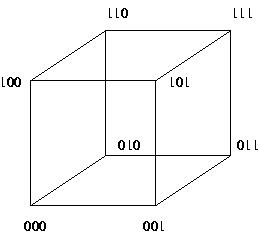
\includegraphics{Images/8cube.jpg} 

It is sometimes helpful to build up a cube from the lower-dimensional
cases.  To build a (d+1)-dimensional cube from two d-dimensional cubes,
just follow this recipe:

\begin{itemize}

\item [(a)] Take a d-dimensional cube and duplicate it. Call these two
cubes subcube 0 and subcube 1. 

\item [(b)] For each pair of same-numbered PEs in the two subcubes, add a
binary digit 0 to the front of the number for the PE in subcube 0, and
add a 1 in the case of subcube 1. Add a link between them. 

\end{itemize}

The following figure shows how a 4-cube can be constructed in this way from
two 3-cubes:

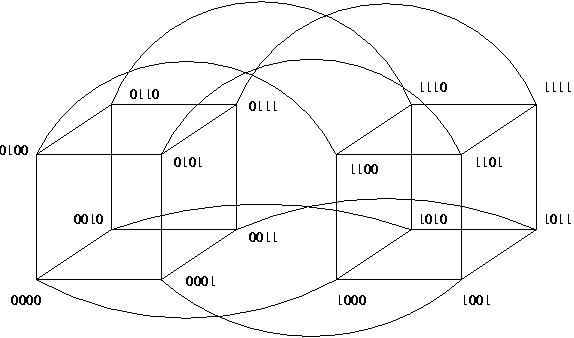
\includegraphics{Images/16cube.jpg} 

Given a PE of number \( (c_{d-1},...,c_{0}) \) in a d-cube, we will
discuss the i-cube to which this PE belongs, meaning all PEs whose first
d-i digits match this PE's.\footnote{Note that this is indeed an
i-dimensional cube, because the last i digits are free to vary.} Of all
these PEs, the one whose last i digits are all 0s is called the
\textbf{root} of this i-cube.

For the 4-cube and PE 1011 mentioned above, for instance, the 2-cube to
which that PE belongs consists of 1000, 1001, 1010 and 1011---i.e. all
PEs whose first two digits are 10---and the root is 1000.

Given a PE, we can split the i-cube to which it belongs into two
(i-1)-subcubes, one consisting of those PEs whose digit i-1 is 0 (to be
called subcube 0), and the other consisting of those PEs whose digit i-1
is 1 (to be called subcube 1).  Each given PE in subcube 0 has as its
\textbf{partner} the PE in subcube 1 whose digits match those of the
given PE, except for digit i-1.

To illustrate this, again consider the 4-cube and the PE 1011. As an
example, let us look at how the 3-cube it belongs to will split into two
2-cubes. The 3-cube to which 1011 belongs consists of 1000, 1001, 1010,
1011, 1100, 1101, 1110 and 1111. This 3-cube can be split into two
2-cubes, one being 1000, 1001, 1010 and 1011, and the other being 1100,
1101, 1110 and 1111. Then PE 1000 is partners with PE 1100, PE 1001 is
partners with PE 1101, and so on.

Each link between two PEs is a dedicated connection, much preferable to
the shared link we have when we run, say, MPI, on a collection of
workstations on an Ethernet. On the other hand, if one PE needs to
communicate with a \underbar{non}-neighbor PE, multiple links (as many
as d of them) will need to be traversed. Thus the nature of the
communications costs here is much different than for a network of
workstations, and this must be borne in mind when developing programs.

\section{Networks of Workstations (NOWs)}

The idea here is simple:  Take a bunch of commodity PCs and network them
for use as parallel processing systems. They are of course individual
machines, capable of the usual uniprocessor, nonparallel applications,
but by networking them together and using message-passing software
environments such as MPI, we can form very powerful parallel systems.

The networking does result in a significant loss of performance, but the
price/performance ratio in NOW can be much superior in many applications
to that of shared-memory or hypercube hardware of comparable number of
CPUs.

\subsection{The Network Is Literally the Weakest Link}

Still, one factor which can be key to the success of a NOW is to use a
fast network, both in terms of hardware and network protocol.  Ordinary
Ethernet and TCP/IP are fine for the applications envisioned by the
original designers of the Internet, e.g. e-mail and file transfer, but
they are slow in the NOW context.  

A popular network for a NOW today is Infiniband (IB)
(\url{www.infinibandta.org}).  It features low latency, about 1.0-3.0
microseconds, high bandwidth, about 1.0-2.0 gigaBytes per second), and
uses a low amount of the CPU's cycles, around 5-10\%.  

The basic building block of IB is a switch, with many inputs and
outputs, similar in concept to $\Omega$-net.  You can build arbitrarily
large and complex topologies from these switches.

A central point is that IB, as with other high-performance networks
designed for NOWs, uses RDMA (Remote Direct Memory Access) read/write,
which eliminates the extra copying of data between the application
program's address space to that of the operating system.

IB has high performance and scalable\footnote{The term {\it
scalable} arises frequently in conversations on parallel processing.  It
means that this particular method of dealing with some aspect of
parallel processing continues to work well as the system size increases.
We say that the method {\it scales}.} implementations of distributed
locks, semaphores, collective communication operations.  An atomic
operation takes about 3-5 microseconds.

IB implements true {\bf multicast}, i.e. the simultaneous sending of
messages to many nodes.  Note carefully that even though MPI has its
{\bf MPI\_Bcast()} function, it will send things out one at a time
unless your network hardware is capable of multicast, and the MPI
implementation you use is configured specifically for that hardware.

For information on network protocols, e.g. for example
\url{www.rdmaconsortium.org}.  A research paper evaluating a tuned
implementation of MPI on IB is available at
\url{nowlab.cse.ohio-state.edu/publications/journal-papers/2004/liuj-ijpp04.pdf}.

\subsection{Other Issues}

Increasingly today, the workstations themselves are multiprocessor
machines, so a NOW really is a hybrid arrangement.  They can be
programmed either purely in a message-passing manner---e.g. running
eight MPI processes on four dual-core machines---or in a mixed way, with
a shared-memory approach being used within a workstation but
message-passing used between them.

NOWs have become so popular that there are now ``recipes'' on how to
build them for the specific purpose of parallel processing.  The term
{\bf Beowulf} come to mean a NOW, usually with a fast network connecting
them, used for parallel processing.  The term {\it NOW} itself is no
longer in use, replaced by {\it cluster}.  Software packages such as
ROCKS (\url{http://www.rocksclusters.org/wordpress/}) have been
developed to make it easy to set up and administer such systems.

\section{Scatter/Gather Operations}
\label{scattergather}

Writing message-passing code is a lot of work, as the programmer must
explicitly arrange for transfer of data.  Contrast that, for instance,
to shared-memory machines, in which cache coherency transactions will
cause data transfers, but which are not arranged by the programmer and
not even seen by him/her.

In order to make coding on message-passing machines easier, higher-level
systems have been devised.  These basically operate in the {\bf
scatter/gather} paradigm, in which a ``manager'' node sends out chunks
of work to the other nodes, serving as ``workers,'' and then collects
and assembles the results sent back the workers.

MPI includes scatter/gather operations in its wide offering of
functions, and they are used in many MPI applications.  R's {\bf snow}
package, which will be discussed in Section \ref{snow}, is based
entirely on scatter/gather, as is MapReduce, to be discussed below.


\chapter{Introduction to MPI} 
\label{chap:mpi}

MPI is the {\it de facto} standard for message-passing software.

\section{Overview}

\subsection{History}

Though (small) shared-memory machines have come down radically in price,
to the point at which a dual-core PC is now commonplace in the home,
historically shared-memory machines were available only to the ``very
rich''---large banks, national research labs and so on.  This led to
interest in message-passing machines.  

The first ``affordable'' message-machine type was the Hypercube,
developed by a physics professor at Cal Tech.  It consisted of a number
of {\bf processing elements} (PEs) connected by fast serial I/O cards.
This was in the range of university departmental research labs.  It was
later commercialized by Intel and NCube.

Later, the notion of {\bf networks of workstations} (NOWs) became
popular.  Here the PEs were entirely independent PCs, connected via a
standard network.  This was refined a bit, by the use of more suitable
network hardware and protocols, with the new term being {\bf clusters}.

All of this necessitated the development of standardized software tools
based on a message-passing paradigm.  The first popular such tool was
Parallel Virtual Machine (PVM).  It still has its adherents today, but
has largely been supplanted by the Message Passing Interface (MPI).

MPI itself later became MPI 2.  Our document here is intended mainly for
the original. 

\subsection{Structure and Execution}

MPI is merely a set of Application Programmer Interfaces (APIs), called
from user programs written in C, C++ and other languages.  It has many
implementations, with some being open source and generic, while others
are proprietary and fine-tuned for specific commercial hardware.

Suppose we have written an MPI program {\bf x}, and will run it on four
machines in a cluster.  Each machine will be running its own copy of
{\bf x}.  Official MPI terminology refers to this as four {\bf
processes}.  Now that multicore machines are commonplace, one might
indeed run two or more cooperating MPI processes---where now we use the
term {\it processes} in the real OS sense---on the same multicore
machine.  In this document, we will tend to refer to the various MPI
processes as {\bf nodes}, with an eye to the cluster setting.

Though the nodes are all running the same program, they will likely be
working on different parts of the program's data.  This is called the
Single Program Multiple Data (SPMD) model.  This is the typical
approach, but there could be different programs running on different
nodes.  Most of the APIs involve a node sending information to, or
receiving information from, other nodes.

\subsection{Implementations}

Two of the most popular implementations of MPI are MPICH and LAM.  MPICH
offers more tailoring to various networks and other platforms, while LAM
runs on networks.  Introductions to MPICH and LAM can be found, for
example, at
\url{http://heather.cs.ucdavis.edu/~matloff/MPI/NotesMPICH.NM.html} and
\url{http://heather.cs.ucdavis.edu/~matloff/MPI/NotesLAM.NM.html},
respectively. 

LAM is no longer being developed, and has been replaced by Open MPI (not
to be confused with OpenMP).  Personally, I still prefer the simplicity
of LAM.  It is still being maintained.

{\bf Note carefully:}  If your machine has more than one MPI
implementation, make absolutely sure one is not interfering with the
other.  Make sure all execution and library paths all include one and
only one implementation at a time.

\subsection{Performance Issues} 

Mere usage of a parallel language on a parallel platform does not
guarantee a performance improvement over a serial version of your
program.  The central issue here is the overhead involved in internode
communication.

Infiniband, one of the fastest cluster networks commercially available,
has a {\bf latency} of about 1.0-3.0 microseconds, meaning that it takes
the first bit of a packet that long to get from one node on an
Infiniband switch to another.  Comparing that to the nanosecond time
scale of CPU speeds, one can see that the communications overhead can
destroy a program's performance.  And Ethernet is quite a bit slower
than Infiniband.

Latency is quite different from {\bf bandwidth}, which is the number of
bits sent per second.  Say the latency is 1.0 microsecond and the
bandwidth is 1 gigabit, i.e. 1000000000 bits per second or 1000 bits
per microsecond.  Say the message is 2000 bits long.  Then the first bit 
of the message arrives after 1 microsecond, and the last bit arrives
after an additional 2 microseconds.  In other words, the message is does
not arrive fully at the destination until 3 microseconds after it is
sent.

In the same setting, say bandwidth is 10 gigabits.  Now the message
would need 1.2 seconds to arrive fully, in spite of a 10-fold increase
in bandwidth.  So latency is a major problem even if the bandwidth is
high.  

For this reason, the MPI applications that run well on networks tend to
be of the ``embarrassingly parallel'' type, with very little
communication between the processes.

Of course, if your platform is a shared-memory multiprocessor
(especially a multicore one, where communication between cores is
particularly fast) and you are running all your MPI processes on that
machine, the problem is less severe.  In fact, some implementations of
MPI communicate directly through shared memory in that case, rather than
using the TCP/IP or other network protocol.

\section{Review of Earlier Example}

Though the presentation in this chapter is self-contained, you may wish
to look first at the somewhat simpler example in Section \ref{mpiex}, a
pipelined prime number finder.

\section{Example:  Dijkstra Algorithm}

\subsection{The Algorithm}

The code implements the Dijkstra algorithm for finding the shortest
paths in an undirected graph.  Pseudocode for the algorithm is

\begin{Verbatim}[fontsize=\relsize{-2},numbers=left]
Done = {0}
NonDone = {1,2,...,N-1}
for J = 1 to N-1 Dist[J] = infinity`
Dist[0] = 0
for Step = 1 to N-1
   find J such that Dist[J] is min among all J in NonDone
   transfer J from NonDone to Done
   NewDone = J
   for K = 1 to N-1
      if K is in NonDone
         Dist[K] = min(Dist[K],Dist[NewDone]+G[NewDone,K])
\end{Verbatim}

At each iteration, the algorithm finds the closest vertex J to 0 among
all those not yet processed, and then updates the list of minimum
distances to each vertex from 0 by considering paths that go through J.
Two obvious potential candidate part of the algorithm for
parallelization are the ``find J'' and ``for K'' lines, and the above
OpenMP code takes this approach.

\subsection{The MPI Code}

\begin{Verbatim}[fontsize=\relsize{-2},numbers=left]
// Dijkstra.c

// MPI example program:  Dijkstra shortest-path finder in a
// bidirectional graph; finds the shortest path from vertex 0 to all
// others

// command line arguments:  nv print dbg

// where:  nv is the size of the graph; print is 1 if graph and min
// distances are to be printed out, 0 otherwise; and dbg is 1 or 0, 1
// for debug

// node 0 will both participate in the computation and serve as a
// "manager"

#include <stdio.h>
#include <mpi.h>

#define MYMIN_MSG 0
#define OVRLMIN_MSG 1
#define COLLECT_MSG 2

// global variables (but of course not shared across nodes)

int nv,  // number of vertices
    *notdone, // vertices not checked yet
    nnodes,  // number of MPI nodes in the computation
    chunk,  // number of vertices handled by each node
    startv,endv,  // start, end vertices for this node
    me,  // my node number 
    dbg; 
unsigned largeint,  // max possible unsigned int
         mymin[2],  // mymin[0] is min for my chunk,
                    // mymin[1] is vertex which achieves that min
         othermin[2],  // othermin[0] is min over the other chunks
                       // (used by node 0 only)
                       // othermin[1] is vertex which achieves that min
         overallmin[2],  // overallmin[0] is current min over all nodes,
                         // overallmin[1] is vertex which achieves that min
         *ohd,  // 1-hop distances between vertices; "ohd[i][j]" is
                // ohd[i*nv+j]
         *mind;  // min distances found so far

double T1,T2;  // start and finish times 

void init(int ac, char **av)
{  int i,j,tmp; unsigned u;
   nv = atoi(av[1]);
   dbg = atoi(av[3]);
   MPI_Init(&ac,&av);
   MPI_Comm_size(MPI_COMM_WORLD,&nnodes);
   MPI_Comm_rank(MPI_COMM_WORLD,&me);
   chunk = nv/nnodes;  
   startv = me * chunk; 
   endv = startv + chunk - 1;
   u = -1;
   largeint = u >> 1;
   ohd = malloc(nv*nv*sizeof(int));
   mind = malloc(nv*sizeof(int));
   notdone = malloc(nv*sizeof(int)); 
   // random graph
   // note that this will be generated at all nodes; could generate just
   // at node 0 and then send to others, but faster this way
   srand(9999);
   for (i = 0; i < nv; i++)  
      for (j = i; j < nv; j++)  {
         if (j == i) ohd[i*nv+i] = 0;
         else  {
            ohd[nv*i+j] = rand() % 20;
            ohd[nv*j+i] = ohd[nv*i+j];
         }
      }
   for (i = 0; i < nv; i++)  {
      notdone[i] = 1;
      mind[i] = largeint;
   }
   mind[0] = 0;
   while (dbg) ;  // stalling so can attach debugger
}

// finds closest to 0 among notdone, among startv through endv
void findmymin()
{  int i;
   mymin[0] = largeint; 
   for (i = startv; i <= endv; i++)
      if (notdone[i] && mind[i] < mymin[0])  {
         mymin[0] = mind[i];
         mymin[1] = i;
      }
}

void findoverallmin()
{  int i;
   MPI_Status status;  // describes result of MPI_Recv() call 
   // nodes other than 0 report their mins to node 0, which receives
   // them and updates its value for the global min
   if (me > 0)  
      MPI_Send(mymin,2,MPI_INT,0,MYMIN_MSG,MPI_COMM_WORLD);
   else  {
      // check my own first
      overallmin[0] = mymin[0];
      overallmin[1] = mymin[1];
      // check the others
      for (i = 1; i < nnodes; i++)  {
         MPI_Recv(othermin,2,MPI_INT,i,MYMIN_MSG,MPI_COMM_WORLD,&status);
         if (othermin[0] < overallmin[0])  {
            overallmin[0] = othermin[0];
            overallmin[1] = othermin[1];
         }
      }
   }
}

void updatemymind()  // update my mind segment
{  // for each i in [startv,endv], ask whether a shorter path to i 
   // exists, through mv
   int i, mv = overallmin[1]; 
   unsigned md = overallmin[0];
   for (i = startv; i <= endv; i++)
      if (md + ohd[mv*nv+i] < mind[i])  
         mind[i] = md + ohd[mv*nv+i];
}

void disseminateoverallmin()
{  int i;
   MPI_Status status;  
   if (me == 0)  
      for (i = 1; i < nnodes; i++)  
         MPI_Send(overallmin,2,MPI_INT,i,OVRLMIN_MSG,MPI_COMM_WORLD);
   else 
      MPI_Recv(overallmin,2,MPI_INT,0,OVRLMIN_MSG,MPI_COMM_WORLD,&status);
}

void updateallmind()  // collects all the mind segments at node 0
{  int i;
   MPI_Status status;  
   if (me > 0)  
      MPI_Send(mind+startv,chunk,MPI_INT,0,COLLECT_MSG,MPI_COMM_WORLD);
   else  
      for (i = 1; i < nnodes; i++)  
         MPI_Recv(mind+i*chunk,chunk,MPI_INT,i,COLLECT_MSG,MPI_COMM_WORLD,
            &status);
}

void printmind()  // partly for debugging (call from GDB)
{  int i;
   printf("minimum distances:\n");
   for (i = 1; i < nv; i++)
      printf("%u\n",mind[i]);
}

void dowork()
{  int step,  // index for loop of nv steps
       i;
   if (me == 0) T1 = MPI_Wtime();
   for (step = 0; step < nv; step++)  {
      findmymin();
      findoverallmin();
      disseminateoverallmin();
      // mark new vertex as done 
      notdone[overallmin[1]] = 0;  
      updatemymind(startv,endv);
   }
   updateallmind();
   T2 = MPI_Wtime();
}

int main(int ac, char **av)
{  int i,j,print;
   init(ac,av);
   dowork();  
   print = atoi(av[2]);
   if (print && me == 0)  {
      printf("graph weights:\n");
      for (i = 0; i < nv; i++)  {
         for (j = 0; j < nv; j++)  
            printf("%u  ",ohd[nv*i+j]);
         printf("\n");
      }
      printmind();
   }
   if (me == 0) printf("time at node 0: %f\n",(float)(T2-T1));
   MPI_Finalize();
}

\end{Verbatim}

The various MPI functions will be explained in the next section.

\subsection{Introduction to MPI APIs}

\subsubsection{MPI\_Init() and MPI\_Finalize()}

These are required for starting and ending execution of an MPI program.
Their actions may be implementation-dependent.  For instance, if our
platform is an Ethernet-based cluster , {\bf MPI\_Init()} will probably
set up the TCP/IP sockets via which the various nodes communicate with
each other.  On an Infiniband-based cluster, connections in the special
Infiniband network protocol will be established.  On a shared-memory
multiprocessor, an implementation of MPI that is tailored to that
platform would take very different actions.

\subsubsection{MPI\_Comm\_size() and MPI\_Comm\_rank()}

In our function {\bf init()} above, note the calls

\begin{Verbatim}[fontsize=\relsize{-2}]
MPI_Comm_size(MPI_COMM_WORLD,&nnodes);
MPI_Comm_rank(MPI_COMM_WORLD,&me);
\end{Verbatim}

The first call determines how many nodes are participating in our
computation, placing the result in our variable {\bf nnodes}.  Here {\bf
MPI\_COMM\_WORLD} is our node group, termed a {\bf communicator} in MPI
parlance.  MPI allows the programmer to subdivide the nodes into groups,
to facilitate performance and clarity of code.  Note that for some
operations, such as barriers, the only way to apply the operation to a
proper subset of all nodes is to form a group.  The totality of all
groups is denoted by {\bf MPI\_COMM\_WORLD}.  In our program here, we
are not subdividing into groups.

The second call determines this node's ID number, called its {\bf rank},
within its group.  As mentioned earlier, even though the nodes are all
running the same program, they are typically working on different parts
of the program's data.  So, the program needs to be able to sense which
node it is running on, so as to access the appropriate data.  Here we
record that information in our variable {\bf me}.

\subsubsection{MPI\_Send()}

To see how MPI's basic send function works, consider our line above,

\begin{Verbatim}[fontsize=\relsize{-2}]
MPI_Send(mymin,2,MPI_INT,0,MYMIN_MSG,MPI_COMM_WORLD);
\end{Verbatim}

Let's look at the arguments:

\begin{itemize}

\item [{\bf mymin:}] 

We are sending a set of bytes.  This argument states the address at
which these bytes begin.

\item [{\bf 2, MPI\_INT:}]

This says that our set of bytes to be sent consists of 2 objects of type
{\bf MPI\_INT}.  That means 8 bytes on 32-bit machines, so why not just
collapse these two arguments to one, namely the number 8?  Why did the
designers of MPI bother to define data types?  The answer is that we
want to be able to run MPI on a heterogeneous set of machines, with MPI
serving as the ``broker'' between them in case different architectures
among those machines handle data differently.

First of all, there is the issue of {\bf endianness}.  Intel machines,
for instance, are {\bf little-endian}, which means that the least
significant byte of a memory word has the smallest address among bytes
of the word.  Sun SPARC chips, on the other hand, are {\bf big-endian},
with the opposite storage scheme.  If our set of nodes included machines
of both types, straight transmission of sequences of 8 bytes might mean
that some of the machines literally receive the data backwards!

Secondly, these days 64-bit machines are becoming more and more common.
Again, if our set of nodes were to include both 32-bit and 64-bit words,
some major problems would occur if no conversion were done.

\item [{\bf 0:}]

We are sending to node 0.

\item [{\bf MYMIN\_MSG:}]

This is the message type, programmer-defined in our line

\begin{Verbatim}[fontsize=\relsize{-2}]
#define MYMIN_MSG 0
\end{Verbatim}

Receive calls, described in the next section, can ask to receive only
messages of a certain type.

\item [{\bf MPI\_COMM\_WORLD:}]

This is the node group to which the message is to be sent.  Above, where
we said we are sending to node 0, we technically should say we are
sending to node 0 within the group {\bf MPI\_COMM\_WORLD}.

\end{itemize}

\subsubsection{MPI\_Recv()}

Let's now look at the arguments for a basic receive:

\begin{Verbatim}[fontsize=\relsize{-2}]
MPI_Recv(othermin,2,MPI_INT,i,MYMIN_MSG,MPI_COMM_WORLD,&status);
\end{Verbatim}

\begin{itemize}

\item [{\bf othermin:}]

The received message is to be placed at our location {\bf othermin}.

\item [{\bf 2,MPI\_INT:}]

Two objects of {\bf MPI\_INT} type are to be received.

\item [{\bf i:}]

Receive only messages from node {\bf i}.  If we did not care what
node we received a message from, we could specify the value
{\bf MPI\_ANY\_SOURCE}.

\item [{\bf MYMIN\_MSG:}]

Receive only messages of type {\bf MYMIN\_MSG}.  If we did not care what
type of message we received, we would specify the value {\bf
MPI\_ANY\_TAG}.

\item [{\bf MPI\_COMM\_WORLD:}]

Group name.

\item [{\bf status:}]

Recall our line

\begin{Verbatim}[fontsize=\relsize{-2}]
MPI_Status status;  // describes result of MPI_Recv() call 
\end{Verbatim}

The type is an MPI {\bf struct} containing information about the
received message.  Its primary fields of interest are {\bf MPI\_SOURCE},
which contains the identity of the sending node, and {\bf MPI\_TAG},
which contains the message type.  These would be useful if the receive
had been done with {\bf MPI\_ANY\_SOURCE} or {\bf MPI\_ANY\_TAG}; the
status argument would then tell us which node sent the message and what
type the message was.

\end{itemize}

\section{Example:  Removing 0s from an Array}

\begin{lstlisting}[numbers=left]
#include <mpi.h>
#include <stdlib.h>

#define MAX_N 100000
#define MAX_NPROCS 100
#define DATA_MSG 0
#define NEWDATA_MSG 1

int nnodes,  // number of MPI processes
    n,  // size of original array
    me,  // my MPI ID
    has0s[MAX_N],  // original data
    no0s[MAX_N],  // 0-free data
    nno0s;  // number of non-0 elements

int debug;

init(int argc, char **argv)
{  
   int i;
   MPI_Init(&argc,&argv);
   MPI_Comm_size(MPI_COMM_WORLD,&nnodes);
   MPI_Comm_rank(MPI_COMM_WORLD,&me);
   n = atoi(argv[1]);
   if (me == 0) {
      for (i = 0; i < n; i++) 
         has0s[i] = rand() % 4;
   } else {
      debug = atoi(argv[2]);
      while (debug) ;
   }
}

void managernode()
{  
   MPI_Status status;
   int i;
   int lenchunk;
   lenchunk = n / (nnodes-1);  // assumed divides evenly
   for (i = 1; i < nnodes; i++) {
      MPI_Send(has0s+(i-1)*lenchunk,lenchunk,
         MPI_INT,i,DATA_MSG,MPI_COMM_WORLD);
   }
   int k = 0;
   for (i = 1; i < nnodes; i++) {
      MPI_Recv(no0s+k,MAX_N,
         MPI_INT,i,NEWDATA_MSG,MPI_COMM_WORLD,&status);
      MPI_Get_count(&status,MPI_INT,&lenchunk);
      k += lenchunk;
   }
   nno0s = k;
}

void remov0s(int *oldx, int n, int *newx, int *nnewx)
{  int i,count = 0;
   for (i = 0; i < n; i++)
      if (oldx[i] != 0) newx[count++] = oldx[i];
   *nnewx = count;
}

void workernode()
{
   int lenchunk;
   MPI_Status status;
   MPI_Recv(has0s,MAX_N,
      MPI_INT,0,DATA_MSG,MPI_COMM_WORLD,&status);
   MPI_Get_count(&status,MPI_INT,&lenchunk);
   remov0s(has0s,lenchunk,no0s,&nno0s);
   MPI_Send(no0s,nno0s,
      MPI_INT,0,NEWDATA_MSG,MPI_COMM_WORLD);
}

int main(int argc,char **argv)
{
   int i;
   init(argc,argv);
   if (me == 0 && n < 25) {
      for (i = 0; i < n; i++) printf("%d ",has0s[i]);
      printf("\n");
   }
   if (me == 0) managernode();
   else workernode();
   if (me == 0 && n < 25) {
      for (i = 0; i < n; i++) printf("%d ",no0s[i]);
      printf("\n");
   }
   MPI_Finalize();
}
\end{lstlisting}

\section{Debugging MPI Code}

If you are using GDB---either directly, or via an IDE such as Eclipse or
Netbeans---the trick with MPI is to {\bf attach} GDB to your running MPI
processes.

Set up code like that we've seen in our examples here:

\begin{lstlisting}[numbers=left]
while (dbg) ;
\end{lstlisting}

This deliberately sets up an infinite loop of {\bf dbg} is nonzero, for
reasons to be discussed below.

For instance, suppose I'm running an MPI program {\bf a.out}, on
machines A, B and C.  I would start the processes as usual, and have 
three terminal windows open.  I'd log in to machine A, find the process
number for {\bf a.out}, using for example a command like {\bf ps ax} on
Unix-family systems, then attach GDB to that process.
Say the process number is 88888.  I'd attach by running the command

\begin{lstlisting}
% gdb a.out 88888
\end{lstlisting}

That would start GDB, in the midst of my already-running process, thus
stuck in the infinite loop seen above.  I hit ctrl-c to interrupt it,
which gives me the GDB prompt, \lstinline{(gdb)}.  I then type

\begin{lstlisting}
(gdb) set var dbg = 0
\end{lstlisting}

which means when I next hit the {\bf c} command in GDB, the program will
proceed, not stuck in the loop anymore.  But first I set my breakpoints.

\section{Collective Communications}

MPI features a number of {\bf collective communication} capabilities, a
number of which are used in the following refinement of our Dijkstra
program:

\subsection{Example:  Refined Dijkstra Code}

\begin{Verbatim}[fontsize=\relsize{-2},numbers=left]
// Dijkstra.coll1.c

// MPI example program:  Dijkstra shortest-path finder in a
// bidirectional graph; finds the shortest path from vertex 0 to all
// others; this version uses collective communication

// command line arguments:  nv print dbg

// where:  nv is the size of the graph; print is 1 if graph and min
// distances are to be printed out, 0 otherwise; and dbg is 1 or 0, 1
// for debug

// node 0 will both participate in the computation and serve as a
// "manager"

#include <stdio.h>
#include <mpi.h>

// global variables (but of course not shared across nodes)

int nv,  // number of vertices
    *notdone, // vertices not checked yet
    nnodes,  // number of MPI nodes in the computation
    chunk,  // number of vertices handled by each node
    startv,endv,  // start, end vertices for this node
    me,  // my node number 
    dbg; 
unsigned largeint,  // max possible unsigned int
         mymin[2],  // mymin[0] is min for my chunk,
                    // mymin[1] is vertex which achieves that min
         overallmin[2],  // overallmin[0] is current min over all nodes,
                         // overallmin[1] is vertex which achieves that min
         *ohd,  // 1-hop distances between vertices; "ohd[i][j]" is
                // ohd[i*nv+j]
         *mind;  // min distances found so far

double T1,T2;  // start and finish times 

void init(int ac, char **av)
{  int i,j,tmp; unsigned u;
   nv = atoi(av[1]);
   dbg = atoi(av[3]);
   MPI_Init(&ac,&av);
   MPI_Comm_size(MPI_COMM_WORLD,&nnodes);
   MPI_Comm_rank(MPI_COMM_WORLD,&me);
   chunk = nv/nnodes;  
   startv = me * chunk; 
   endv = startv + chunk - 1;
   u = -1;
   largeint = u >> 1;
   ohd = malloc(nv*nv*sizeof(int));
   mind = malloc(nv*sizeof(int));
   notdone = malloc(nv*sizeof(int)); 
   // random graph
   // note that this will be generated at all nodes; could generate just
   // at node 0 and then send to others, but faster this way
   srand(9999);
   for (i = 0; i < nv; i++)  
      for (j = i; j < nv; j++)  {
         if (j == i) ohd[i*nv+i] = 0;
         else  {
            ohd[nv*i+j] = rand() % 20;
            ohd[nv*j+i] = ohd[nv*i+j];
         }
      }
   for (i = 0; i < nv; i++)  {
      notdone[i] = 1;
      mind[i] = largeint;
   }
   mind[0] = 0;
   while (dbg) ;  // stalling so can attach debugger
}

// finds closest to 0 among notdone, among startv through endv
void findmymin()
{  int i;
   mymin[0] = largeint; 
   for (i = startv; i <= endv; i++)
      if (notdone[i] && mind[i] < mymin[0])  {
         mymin[0] = mind[i];
         mymin[1] = i;
      }
}

void updatemymind()  // update my mind segment
{  // for each i in [startv,endv], ask whether a shorter path to i 
   // exists, through mv
   int i, mv = overallmin[1]; 
   unsigned md = overallmin[0];
   for (i = startv; i <= endv; i++)
      if (md + ohd[mv*nv+i] < mind[i])  
         mind[i] = md + ohd[mv*nv+i];
}

void printmind()  // partly for debugging (call from GDB)
{  int i;
   printf("minimum distances:\n");
   for (i = 1; i < nv; i++)
      printf("%u\n",mind[i]);
}

void dowork()
{  int step,  // index for loop of nv steps
       i;
   if (me == 0) T1 = MPI_Wtime();
   for (step = 0; step < nv; step++)  {
      findmymin();
      MPI_Reduce(mymin,overallmin,1,MPI_2INT,MPI_MINLOC,0,MPI_COMM_WORLD);
      MPI_Bcast(overallmin,1,MPI_2INT,0,MPI_COMM_WORLD);
      // mark new vertex as done 
      notdone[overallmin[1]] = 0;  
      updatemymind(startv,endv);
   }
   // now need to collect all the mind values from other nodes to node 0
   MPI_Gather(mind+startv,chunk,MPI_INT,mind,chunk,MPI_INT,0,MPI_COMM_WORLD);
   T2 = MPI_Wtime();
}

int main(int ac, char **av)
{  int i,j,print;
   init(ac,av);
   dowork();  
   print = atoi(av[2]);
   if (print && me == 0)  {
      printf("graph weights:\n");
      for (i = 0; i < nv; i++)  {
         for (j = 0; j < nv; j++)  
            printf("%u  ",ohd[nv*i+j]);
         printf("\n");
      }
      printmind();
   }
   if (me == 0) printf("time at node 0: %f\n",(float)(T2-T1));
   MPI_Finalize();
}
\end{Verbatim}

The new calls will be explained in the next section.

\subsection{MPI\_Bcast()}

In our original Dijkstra example, we had a loop

\begin{Verbatim}[fontsize=\relsize{-2}]
for (i = 1; i < nnodes; i++)  
   MPI_Send(overallmin,2,MPI_INT,i,OVRLMIN_MSG,MPI_COMM_WORLD);
\end{Verbatim}

in which node 0 sends to all other nodes.  We can replace this by

\begin{Verbatim}[fontsize=\relsize{-2}]
MPI_Bcast(overallmin,2,MPI_INT,0,MPI_COMM_WORLD);
\end{Verbatim}

In English, this call would say, 

\begin{quote}

At this point all nodes participate in a broadcast operation, in which
node 0 sends 2 objects of type {\bf MPI\_INT} to each node (including
itself).  The source of the data will be located at address {\bf
overallmin} at node 0, and the other nodes will receive the data at a
location of that name.

\end{quote}

Note my word ``participate'' above.  The name of the function is
``broadcast,'' which makes it sound like only node 0 executes this line
of code, which is not the case; all the nodes in the group (in this
case that means all nodes in our entire computation) execute this line.
The only difference is the action; most nodes participate by receiving,
while node 0 participates by sending.

Actually, this call to {\bf MPI\_Bcast()} is doing more than replacing
the loop, since the latter had been part of an if-then-else that checked
whether the given process had rank 0 or not.

Why might this be preferable to using an explicit loop?  First, it would
obviously be much clearer.  That makes the program easier to write,
easier to debug, and easier for others (and ourselves, later) to read.

But even more importantly, using the broadcast may improve performance.
We may, for instance, be using an implementation of MPI which is
tailored to the platform on which we are running MPI.  If for instance
we are running on a network designed for parallel computing, such as
Myrinet or Infiniband, an optimized broadcast may achieve a much higher
performance level than would simply a loop with individual send calls.
On a shared-memory multiprocessor system, special machine instructions
specific to that platform's architecture can be exploited, as for
instance IBM has done for its shared-memory machines.  Even on an
ordinary Ethernet, one could exploit Ethernet's own broadcast mechanism,
as had been done for PVM, a system like MPI (G. Davies and N. Matloff,
Network-Specific Performance Enhancements for PVM, {\it Proceedings  of
the  Fourth IEEE International Symposium on High-Performance Distributed
Computing}, 1995, 205-210; N. Matloff, Analysis of a Programmed Backoff
Method for Parallel Processing on Ethernets, in {\it Network-Based
Parallel Computing}).

\subsection{MPI\_Reduce()/MPI\_Allreduce()}
\label{mpireduction}

Look at our call

\begin{Verbatim}[fontsize=\relsize{-2}]
MPI_Reduce(mymin,overallmin,1,MPI_2INT,MPI_MINLOC,0,MPI_COMM_WORLD);
\end{Verbatim}

above.  In English, this would say,

\begin{quote} At this point all nodes in this group participate in a
``reduce'' operation.  The type of reduce operation is {\bf
MPI\_MINLOC}, which means that the minimum value among the nodes will be
computed, and the index attaining that minimum will be recorded as well.
Each node contributes a value to be checked, and an associated index,
from a location {\bf mymin} in their programs; the type of the pair is
{\bf MPI\_2INT}.  The overall min value/index will be computed by
combining all of these values at node 0, where they will be placed at a
location {\bf overallmin}.  \end{quote}

MPI also includes a function {\bf MPI\_Allreduce()}, which does the same
operation, except that instead of just depositing the result at one
node, it does so at all nodes.  So for instance our code above,

\begin{Verbatim}[fontsize=\relsize{-2}]
MPI_Reduce(mymin,overallmin,1,MPI_2INT,MPI_MINLOC,0,MPI_COMM_WORLD);
MPI_Bcast(overallmin,1,MPI_2INT,0,MPI_COMM_WORLD);
\end{Verbatim}

could be replaced by

\begin{Verbatim}[fontsize=\relsize{-2}]
MPI_Allreduce(mymin,overallmin,1,MPI_2INT,MPI_MINLOC,MPI_COMM_WORLD);
\end{Verbatim}

Again, these can be optimized for particular platforms.

Here is a table of MPI reduce operations:

\begin{tabular}{|r|r|}
\hline
MPI\_MAX & max \\
MPI\_MIN & min \\
MPI\_SUM & sum \\
MPI\_PROD & product \\
MPI\_LAND & wordwise boolean and \\
MPI\_LOR & wordwise boolean or \\
MPI\_LXOR & wordwise exclusive or \\
MPI\_BAND & bitwise boolean and \\
MPI\_BOR & bitwise boolean or \\
MPI\_BXOR & bitwise exclusive or \\
MPI\_MAXLOC & max value and location \\
MPI\_MINLOC & min value and location \\
\hline
\end{tabular}

\subsection{MPI\_Gather()/MPI\_Allgather()}

A classical approach to parallel computation is to first break the data for
the application into chunks, then have each node work on its chunk, and
then gather all the processed chunks together at some node.  The MPI
function {\bf MPI\_Gather()} does this.

In our program above, look at the line

\begin{Verbatim}[fontsize=\relsize{-2}]
MPI_Gather(mind+startv,chunk,MPI_INT,mind,chunk,MPI_INT,0,MPI_COMM_WORLD);
\end{Verbatim}

In English, this says,

\begin{quote}

At this point all nodes participate in a gather operation, in which each
node (including Node 0) contributes {\bf chunk} number of MPI integers,
from a location {\bf mind+startv} in that node's program.  Node 0 then
receives {\bf chunk} items sent from each node, stringing everything together
in node order and depositing it all at {\bf mind} in the program running
at Node 0.

\end{quote}

(Yes, the fifth argument is redundant with the second; same for the
thrid and sixth.)

There is also {\bf MPI\_Allgather()}, which places the result at all
nodes, not just one.  Its call form is the same as {\bf MPI\_Gather()},
but with one fewer argument (since the identity of ``the'' gathering
node is no longer meaningful):

\begin{lstlisting}
int MPI_Allgather(srcbuf, srccount, srctype, destbuf, destcount, desttype, communicator)
\end{lstlisting}

\subsection{The MPI\_Scatter()}

This is the opposite of {\bf MPI\_Gather()}, i.e. it breaks long data
into chunks which it parcels out to individual nodes.  For example,
in the code in the next section, the call

\begin{lstlisting}
MPI_Scatter(oh, lenchunk, MPI_INT, ohchunk, lenchunk, MPI_INT, 0,
   MPI_COMM_WORLD);
\end{lstlisting} 

means

\begin{quote}
Node 0 will break up the array {\bf oh} of type MPI\_INT into chunks 
of length {\bf lenchunk}, sending the i$^{th}$ chunk to Node i, where
{\bf lenchunk} items will be deposited at {\bf ohchunk}.
\end{quote}

\subsection{Example:  Count the Number of Edges in a Directed Graph}

Below is MPI code to count the number of edges in a directed graph.
(``Directed'' means that a link from i to j does not necessarily imply
one from j to i.)  

In the context here, {\bf me} is the node's rank; {\bf nv} is the number
of vertices; {\bf oh} is the one-hop distance matrix; and {\bf nnodes}
is the number of MPI processes.  At the beginning only the process of
rank 0 has a copy of {\bf oh}, but it sends that matrix out in chunks to
the other nodes, each of which stores its chunk in an array {\bf
ohchunk}. 

\begin{lstlisting}[numbers=left]
lenchunk = nv / nnodes;
MPI_Scatter(oh, lenchunk, MPI_INT, ohchunk, lenchunk, MPI_INT, 0,
   MPI_COMM_WORLD);
mycount = 0;
for (i = 0; i < nv*nv/nnodes)
   if (ohchunk[i] != 0) mycount++;
MPI_Reduce(&mycount,&numedge,1,MPI_INT,MPI_SUM,0,MPI_COMM_WORLD);
if (me == 0) printf("there are %d edges\n",numedge);
\end{lstlisting}

\subsection{Example:  Cumulative Sums}

Here we find cumulative sums.  For instance, if the original array is
(3,1,2,0,3,0,1,2), then it is changed to (3,4,6,6,9,9,10,12).  (This
topic is pursued in depth in Chapter \ref{chap:prefix}.)

\begin{lstlisting}[numbers=left]
// finds cumulative sums in the array x

#include <mpi.h>
#include <stdlib.h>

#define MAX_N 10000000  
#define MAX_NODES 10

int nnodes,  // number of MPI processes
    n,  // size of x
    me,  // MPI rank of this node
    // full data for node 0, part for the rest
    x[MAX_N],  
    csums[MAX_N],  // cumulative sums for this node
    maxvals[MAX_NODES];  // the max values at the various nodes 

int debug; 

init(int argc, char **argv)
{  
   int i;
   MPI_Init(&argc,&argv);
   MPI_Comm_size(MPI_COMM_WORLD,&nnodes);
   MPI_Comm_rank(MPI_COMM_WORLD,&me); 
   n = atoi(argv[1]); 
   // test data
   if (me == 0) {
      for (i = 0; i < n; i++) 
         x[i] = rand() % 32;
   } 
   debug = atoi(argv[2]); 
   while (debug) ;
}

void cumulsums()
{  
   MPI_Status status;
   int i,lenchunk,sum,node; 
   lenchunk = n / nnodes;  // assumed to divide evenly
   // note that node 0 will participate in the computation too
   MPI_Scatter(x,lenchunk,MPI_INT,x,lenchunk,MPI_INT,
      0,MPI_COMM_WORLD);
   sum = 0;
   for (i = 0; i < lenchunk; i++) {
      csums[i] = sum + x[i];
      sum += x[i];
   }
   MPI_Gather(&csums[lenchunk-1],1,MPI_INT,
      maxvals,1,MPI_INT,0,MPI_COMM_WORLD);
   MPI_Bcast(maxvals,nnodes,MPI_INT,0,MPI_COMM_WORLD);
   if (me > 0) {
      sum = 0;
      for (node = 0; node < me; node++) {
         sum += maxvals[node];
      }
      for (i = 0; i < lenchunk; i++) 
         csums[i] += sum;
   }
   MPI_Gather(csums,lenchunk,MPI_INT,csums,lenchunk,MPI_INT,
      0,MPI_COMM_WORLD);
}

int main(int argc,char **argv)
{  
   int i;
   init(argc,argv);
   if (me == 0 && n < 25) {
      for (i = 0; i < n; i++) printf("%d ",x[i]);
      printf("\n");
   }
   cumulsums();
   if (me == 0 && n < 25) {
      for (i = 0; i < n; i++) printf("%d ",csums[i]);
      printf("\n");
   }
   MPI_Finalize();
}
\end{lstlisting}

\subsection{Example:  an MPI Solution to the Mutual Outlinks Problem}

Consider the example of Section \ref{mutlinks}.  We have
a network graph of some kind, such as Web links.  For any two
vertices, say any two Web sites, we might be interested in mutual
outlinks, i.e. outbound links that are common to two Web sites.

The MPI code below finds the mean number of mutual outlinks, among
all pairs of vertices in a graph.

\begin{lstlisting}[numbers=left]
// MPI solution to the mutual outlinks problem

// adjacency matrix m is global at each node, broadcast from node 0

// assumes m is nxn, and number of nodes is < n

// for each node i, check all possible pairing nodes j > i; the various
// nodes work on values of i in a Round Robin fashion, with node k
// handling all i for which i mod nnodes = k

#include <mpi.h>
#include <stdlib.h>

#define MAXLENGTH 10000000  

int nnodes,  // number of MPI processes
    n,  // size of x
    me,  // MPI rank of this node
    m[MAXLENGTH],  // adjacency matrix
    grandtot;  // grand total of all counts of mutuality

// get adjacency matrix, in this case just by simulation
void getm() 
{  int i;
   for (i = 0; i < n*n; i++) 
      m[i] = rand() % 2;
}

init(int argc, char **argv)
{  
   int i;
   MPI_Init(&argc,&argv);
   MPI_Comm_size(MPI_COMM_WORLD,&nnodes);
   MPI_Comm_rank(MPI_COMM_WORLD,&me); 
   n = atoi(argv[1]); 
   if (me == 0) {
      getm();  // get the data (app-specific)
   } 
}

void mutlinks()
{  
   int i,j,k,tot; 
   MPI_Bcast(m,n*n,MPI_INT,0,MPI_COMM_WORLD);
   tot = 0;
   for (i = me; i < n-1; i += nnodes) {
      for (j = i+1; j < n; j++) {
         for (k = 0; k < n; k++) 
            tot += m[twod2oned(n,i,k)] * m[twod2oned(n,j,k)];
      }
   }
   MPI_Reduce(&tot,&grandtot,1,MPI_INT,MPI_SUM,0,MPI_COMM_WORLD);
}

// convert 2-D subscript to 1-D
int twod2oned(n,i,j) 
{  return n * i + j;  }

int main(int argc,char **argv)
{  int i,j;
   init(argc,argv);
   if (me == 0 && n < 5) {  // check test input
      for (i = 0; i < n; i++) {
         for (j = 0; j < n; j++) printf("%d ",m[twod2oned(n,i,j)]);
         printf("\n");
      }
   }
   mutlinks();
   if (me == 0) printf("%f\n",((float) grandtot)/(n*(n-1)/2));
   MPI_Finalize();
}
\end{lstlisting}

\subsection{The MPI\_Barrier()}  

This implements a barrier for a given communicator.  The name of the
communicator is the sole argument for the function.  

Explicit barriers are less common in message-passing programs than in
the shared-memory world.

\subsection{Creating Communicators} 

Again, a communicator is a subset (either proper or improper) of all of
our nodes.  MPI includes a number of functions for use in creating
communicators.  Some set up a virtual ``topology'' among the nodes.  

For instance, many physics problems consist of solving differential
equations in two- or three-dimensional space, via approximation on a
grid of points.  In two dimensions, groups may consists of rows in the
grid.

Here's how we might divide an MPI run into two groups (assumes an even
number of MPI processes to begin with):

\begin{Verbatim}[fontsize=\relsize{-2}]
MPI_Comm_size(MPI_COMM_WORLD,&nnodes);
MPI_Comm_rank(MPI_COMM_WORLD,&me);
...
// declare variables to bind to groups
MPI_Group worldgroup, subgroup; 
// declare variable to bind to a communicator
MPI_Comm subcomm; 
...
int i,startrank,nn2 = nnodes/2;
int *subranks = malloc(nn2*sizeof(int));
if (me < nn2) start = 0;
else start = nn2;
for (i = 0; i < nn2; i++) 
   subranks[i] = i + start;
// bind the world to a group variable
MPI_Comm_group(MPI_COMM_WORLD, &worldgroup); 
// take worldgroup the nn2 ranks in "subranks" and form group 
// "subgroup" from them 
MPI_Group_incl(worldgroup, nn2, subranks, subgroup);
// create a communicator for that new group
MPI_Comm_create(MPI_COMM_WORLD, subgroup, subcomm); 
// get my rank in this new group
MPI_Group_rank (subgroup, &subme); 
\end{Verbatim}

You would then use {\bf subcomm} instead of MPI\_COMM\_WORLD
whenever you wish to, say, broadcast, only to that group.

\section{Buffering, Synchrony and Related Issues}

As noted several times so far, interprocess communication in parallel
systems can be quite expensive in terms of time delay.  In this section
we will consider some issues which can be extremely important in this
regard.

\subsection{Buffering, Etc.}

To understand this point, first consider situations in which MPI is
running on some network, under the TCP/IP protocol.  Say an MPI program
at node A is sending to one at node B.

It is extremely import to keep in mind the levels of abstraction here.
The OS's TCP/IP stack is running at the Session, Transport and Network
layers of the network.  MPI---meaning the MPI internals---is running
above the TCP/IP stack, in the Application layers at A and B.  And the
MPI user-written application could be considered to be running at a
``Super-application'' layer, since it calls the MPI internals.  (From
here on, we will refer to the MPI internals as simply ``MPI.'')

MPI at node A will have set up a TCP/IP socket to B during the user
program's call to {\bf MPI\_Init()}.  The other end of the socket will
be a corresponding one at B.  This setting up of this socket pair as
establishing a {\bf connection} between A and B.  When node A calls {\bf
MPI\_Send()}, MPI will write to the socket, and the TCP/IP stack will
transmit that data to the TCP/IP socket at B.  The TCP/IP stack at B
will then send whatever bytes come in to MPI at B.

Now, it is important to keep in mind that in TCP/IP the totality of
bytes sent by A to B during lifetime of the connection is considered one
long message.  So for instance if the MPI program at A calls {\bf
MPI\_Send()} five times, the MPI internals will write to the socket five
times, but the bytes from those five messages will not be perceived by
the TCP/IP stack at B as five messages, but rather as just one long
message (in fact, only part of one long message, since more may be yet
to come).

MPI at B continually reads that ``long message'' and breaks it back into
MPI messages, keeping them ready for calls to {\bf MPI\_Recv()} from the
MPI application program at B.  Note carefully that phrase, {\it keeping
them ready}; it refers to the fact that the order in which the MPI
application program requests those messages may be different from the
order in which they arrive.

On the other hand, looking again at the TCP/IP level, even though all
the bytes sent are considered one long message, it will physically be
sent out in pieces.  These pieces don't correspond to the pieces written
to the socket, i.e. the MPI messages.  Rather, the breaking into pieces
is done for the purpose of {\bf flow control}, meaning that the TCP/IP
stack at A will not send data to the one at B if the OS at B has no room
for it.  The {\bf buffer} space the OS at B has set up for receiving
data is limited.  As A is sending to B, the TCP layer at B is telling
its counterpart at A when A is allowed to send more data.  

Think of what happens the MPI application at B calls {\bf MPI\_Recv()},
requesting to receive from A, with a certain tag T.  Say the first
argument is named {\bf x}, i.e.  the data to be received is to be
deposited at {\bf x}.  If MPI sees that it already has a message of tag
T, it will have its {\bf MPI\_Recv()} function return the message to the
caller, i.e. to the MPI application at B.  {\bf If no such message has
arrived yet, MPI won't return to the caller yet, and thus the caller
blocks.}

{\bf MPI\_Send()} can block too.  If the platform and MPI implementation
is that of the TCP/IP network context described above, then the send
call will return when its call to the OS' {\bf write()} (or equivalent,
depending on OS) returns, but that could be delayed if the OS' buffer
space is full.  On the other hand, another implementation could require
a positive response from B before allowing the send call to return.

%  \subsection{Nonbuffered Communication}
%  
%  The above analysis applies to MPI applications that run on top of
%  TCP/IP, with a natural buffering system.  In fact, there is likely
%  additional buffering as well.  By contrast, some other platforms may not
%  have any buffering at all.  This is not the usual situation, but it
%  could be the case, for instance, when the underlying platform is a
%  shared-memory multiprocessor and the MPI implementation takes advantage
%  of that structure, rather than just using TCP/IP.

Note that buffering slows everything down.  In our TCP scenario above,
{\bf MPI\_Recv()} at B must copy messages from the OS' buffer space to
the MPI application program's program variables, e.g.  {\bf x} above.
This is definitely a blow to performance.  That in fact is why networks
developed specially for parallel processing typically include mechanisms
to avoid the copying.  Infiniband, for example, has a Remote Direct
Memory Access capability, meaning that A can write directly to {\bf x}
at B.  Of course, if our implementation uses {\bf synchronous}
communication, with A's send call not returning until A gets a response
from B, we must wait even longer.

Technically, the MPI standard states that {\bf MPI\_Send(x,...)} will
return only when it is safe for the application program to write over
the array which it is using to store its message, i.e. {\bf x}.  As we
have seen, there are various ways to implement this, with performance
implications.  Similarly, {\bf MPI\_Recv(y,...)} will return only when
it is safe to read {\bf y}.

%  So, we may either have a no-buffering situation forced upon us, or may
%  opt for no buffering for performance reasons.  But that has a big
%  implication:  Node A cannot call {\bf MPI\_Send()} until node B has
%  called {\bf MPI\_Recv()}; otherwise B may be using the space at {\bf x}, 
%  in which case A's premature {\bf MPI\_Send()} would ruin things at that
%  location.  That would mean that B would have to inform A when it calls
%  {\bf MPI\_Recv()}.  This is called {\bf synchronous} communication.
%  Clearly, this can be a major cause of slowdown if not handled carefully.

\subsection{Safety}

With {\bf synchronous} communication, deadlock is a real risk.  Say A
wants to send two messages to B, of types U and V, but that B wants to
receive V first.  Then A won't even get to send V, because in preparing
to send U it must wait for a notice from B that B wants to read U---a
notice which will never come, because B sends such a notice for V first.
This would not occur if the communication were asynchronous.

But beyond formal deadlock, programs can fail in other ways, even with
buffering, as buffer space is always by nature finite.  A program can
fail if it runs out of buffer space, either at the sender or the
receiver.  See
\url{www.llnl.gov/computing/tutorials/mpi_performance/samples/unsafe.c}
for an example of a test program which demonstrates this on a certain
platform, by deliberating overwhelming the buffers at the receiver.

In MPI terminology, asynchronous communication is considered {\bf
unsafe}.  The program may run fine on most systems, as most systems are
buffered, but fail on some systems.  Of course, as long as you know your
program won't be run in nonbuffered settings, it's fine, and since there
is potentially such a performance penalty for doing things
synchronously, most people are willing to go ahead with their ``unsafe''
code.

\subsection{Living Dangerously}

If one is sure that there will be no problems of buffer overflow and so
on, one can use variant send and receive calls provided by MPI, such as
{\bf MPI\_Isend()} and {\bf MPI\_Irecv()}.  The key difference between
them and {\bf MPI\_Send()} and {\bf MPI\_Recv()} is that they return
immediately, and thus are termed {\bf nonblocking}.  Your code can go on
and do other things, not having to wait.

This does mean that at A you cannot touch the data you are sending until
you determine that it has either been buffered somewhere or has reached
{\bf x} at B.  Similarly, at B you can't use the data at {\bf x} until
you determine that it has arrived.  Such determinations can be made via
{\bf MPI\_Wait()}.  In other words, you can do your send or receive,
then perform some other computations for a while, and then call {\bf
MPI\_Wait()} to determine whether you can go on.  Or you can call {\bf
MPI\_Probe()} to ask whether the operation has completed yet.

\subsection{Safe Exchange Operations}

In many applications A and B are swapping data, so both are sending and
both are receiving.  This too can lead to deadlock.  An obvious solution
would be, for instance, to have the lower-rank node send first and the
higher-rank node receive first.  

But a more convenient, safer and possibly faster alternative would be to
use MPI's {\bf MPI\_Sendrecv()} function.  Its prototype is

\begin{Verbatim}[fontsize=\relsize{-2}]
intMPI_Sendrecv_replace(void* buf, int count, MPI_Datatype datatype, 
   int dest, int sendtag, int source, int recvtag, MPI_Comm comm, 
   MPI_Status *status) 
\end{Verbatim}

Note that the sent and received messages can be of different lengths and
can use different tags.

\section{Use of MPI from Other Languages}

MPI is a vehicle for parallelizing C/C++, but some clever people have
extended the concept to other languages, such as the cases of Python and
R that we treat in Chapters \ref{chap:pythr} and \ref{chap:r}.

\section{Other MPI Examples in This Book}

\begin{itemize}

\item The pipelined prime number finder in Chapter \ref{chap:intro}.

\item Bucket sort with sampling, in Section \ref{bsort}.

\end{itemize}




\include{./chapter/hadoop}
\chapter{R 并行处理入门}
\label{chap:r}

\section{为什么要在本书中用 R 语言?}

在本书的其它章节里,C/C++依然是我们的主要语言,但我们也提供
很多 R 语言的示例。为什么要用 R 呢?

\begin{itemize}

\item R 是最广泛使用的用于统计分析和数据处理的编程语言。在现今
这个大数据时代,人民已经开发了相当数量的用于并行计算的 R 扩展包。
特别地,{\bf parallel} 扩展包现在已经是 R 基础包的一部分。

\item R 语言的广泛使用,从 Google 设置了其内部的 R 语言规范一事
就可见一斑\footnote{个人角度来讲,我并不喜欢这些代码规范,
我更喜欢我自己的。但从 Google 设置
自己的 R 语言规范可以看出他们对 R 的重视程度。}。现在 Oracle 也
把 R 包含了自己的大数据分析方案中。

\item 对于展示各种各样的并行算法,R 非常方便。这点的主要原因
在于 R 内置了向量、矩阵和复数类型。

\end{itemize}

Python 也有很多并行库,比如 {\bf multiprocessing}。关于 Python 的
并行话题,我们会在第\ref{chap:pythr}章里讨论。

{\bf 本章的示例会保持尽量简单。}但 R 中的并行计算也可以应用到非常庞大
而复杂的问题上。在附录\ref{chap:rquickstart}中,有一个5分钟的 R 快速入门。
阅读时请牢记 R 中 list 结构。

{\bf R 中进行并行计算的关键就是—— list 结构的操作。}许多 R 的并行计算
扩展包都非常依赖于 R 中的 list 结构。输入输出的参数和返回值经常
都采用 list 的形式。读者可能有
兴趣参考一下附录\ref{chap:rquickstart}中的相关内容。

\section{R 和易并行问题(Embarrassing Parallel Problems)}

需要注意的是,R 的并行扩展包一般只能处理易并行问题。正如在
\ref{embpar}节中定义的,这些问题不仅容易并行化,而且信息传递
的需求很少\footnote{后面的要求把很多迭代算法排除在外了,
尽管它们很容易并行化。}。如我们所知,一般只有易并行问题会有
很好的表现,但在 R 中情况尤其如此,原因如下。

R 语言的函数式编程的本质意味着,任何对一个向量或矩阵的元素的写入操作,
比如
\begin{lstlisting}
x[3] <- 8
\end{lstlisting}
都会重写整个向量或矩阵\footnote{R 中的元素赋值是一个函数调用,
上面这个例子的参数分别为 {\bf x}、3和8。}。虽然有些例外(随着 R 版本
更新,例外可能越来越多),但一般来说我们必须承认 R 中并行的向量
和矩阵代码代价很高\footnote{R 中新的引用类(Reference class)可能会对此有所改变。}。

对于不易并行的问题,大家应该考虑用 R 调用并行的 C 代码,这点会在\ref{cfromr}
节中讨论。

\section{一些 R 的并行扩展包}

这里我们列举了一些 R 的并行扩展包:

\begin{itemize}

\item Message-passing 或 scatter/gather (\ref{scattergather}节):
{\bf Rmpi}、{\bf snow}、{\bf foreach}、{\bf rmr}、{\bf Rhipe}、{\bf multicore}\footnote{{\bf multicore} 扩展包运行于多核
内存共享的平台之上,但在读写过程中并不共享数据。}、{\bf rzmq}

\item 内存共享:{\bf Rdsm}、{\bf bigmemory}

\item GPU:{\bf gputools}、{\bf rgpu}

\end{itemize}

大家可以从
\url{http://cran.r-project.org/web/views/HighPerformanceComputing.html}找到更加详尽
的列表。

从2.14版本开始,R 默认包括了由 {\bf snow} 和 {\bf multicore} 构成
的 {\bf parallel} 扩展包。(早期版本可能需要分别下载。)
正是因为如此,二者都在范围之内。另外,我们也会讨论
{\bf Rdsm/bigmemory} 和 {\bf gputools}。

\section{安装和载入这些扩展包}

{\bf 安装:}

需要注意的是,如果你使用的是2.14版或更高版本的 R,你已经安装
了 {\bf snow} 和 {\bf multicore}。一般来说,除了 {\bf rgpu},
其它所有扩展包都可以从 R 官方的代码仓库 CRAN\url{http://cran.r-project.org})下载。
这里以 {\bf snow} 为例:

加入你想把它安装在 {\bf /a/b/c/} 目录下。最简单的方法就是
使用 R 的函数:

\begin{lstlisting}
> install.packages("snow","/a/b/c/")
\end{lstlisting}

这会将 {\bf snow} 安装在 {\bf /a/b/c/{\bf snow}} 目录下。

之后你需要将目录{\bf /a/b/c}(不是{\bf
/a/b/c/snow})加到你的 R 搜索路径中。我推荐大家在
自己 home 目录下的{\bf .Rprofile}文件(这是 R 的启动设置文件)中添加这样一行。
\begin{lstlisting}
.libPaths("/a/b/c/")
\end{lstlisting}

在一些情况下,由于所需库的位置原因,你可能需要手动安装一个 CRAN 上的扩展包。
这一点请参考下面的\ref{gpuinstall}节和\ref{rgpu}节。

{\bf 载入一个扩展包:}

通过调用 {\bf library()} 来载入一个扩展包。
例如,载入{\bf parallel},可以使用:
\begin{lstlisting}
> library(parallel)
\end{lstlisting}

\section{R 中的 snow 扩展包}
\label{snow}

{\bf snow}最大的优点在于其简单。其概念和实现都非常简单,
能出错的地方不多。因此,它可能是现在使用最广泛的 R 并行包。


{\bf snow} 扩展包可以直接通过network socket运行
(由于用户只需要安装{\bf snow},着可能是最常见的用法),
也可以运行于{\bf Rmpi}(R 的 MPI 接口)、PVM 或 NWS之上。

它也可以在一个 scatter/gather 模型(\ref{scattergather}节)下
进行操作。正如 R 中的{\bf apply()}函数会将同样的函数作用于
一个矩阵的每行上(见下面的示例),{\bf snow}中
的{\bf parApply()}会在多台机器上并行地完成类似的操作;
不同的机器会操作不同的行。(除了使用多台机器,我们也可以
在多核的机器上运行多个{\bf snow} client。)

\subsection{使用}

After loading {\bf snow}, by typing

\begin{lstlisting}
> library(snow)
\end{lstlisting}

one sets up a {\bf snow} cluster, by calling the {\bf snow} function
{\bf makeCluster()}.  The named argument {\bf type} of that function
indicates the networking platform, e.g. ``MPI'' or ``SOCK." The last
indicates that you wish {\bf snow} to run on TCP/IP sockets that it
creates itself, rather than going through MPI etc.

In the examples here, I used ``SOCK,'' on machines named {\bf pc48} and
{\bf pc49}, setting up the cluster this way:\footnote{If you are on a
shared-file system group of machines, try to stick to ones for which the
path to R is the same for all, to avoid problems.}

\begin{lstlisting}
> cls <- makeCluster(type="SOCK",c("pc48","pc49"))
\end{lstlisting}

Note that the above R code sets up {\bf worker nodes} at the machines
named {\bf pc48} and {\bf pc49}; these are in addition to the {\bf
manager node}, which is the machine on which that R code is
executed.

By the way, if you want to make worker nodes on the same machine as the
manager (typically on a multicore machine), use {\bf localhost} as the
machine name.

There are various other optional arguments.  One you may find useful is
{\bf outfile}, which records the result of the call in the file {\bf
outfile}.  This can be helpful for debugging if the call fails.

\subsection{示例:使用 parApply() 进行矩阵向量相乘}

To introduce {\bf snow}, consider a simple example of multiplication of
a vector by a matrix.  We set up a test matrix:

\begin{lstlisting}[numbers=left]
> a <- matrix(c(1:12),nrow=6)
> a
     [,1] [,2]
[1,]    1    7
[2,]    2    8
[3,]    3    9
[4,]    4   10
[5,]    5   11
[6,]    6   12
\end{lstlisting}

We will multiply the vector $(1,1)^{T}$ (T meaning transpose) by our
matrix {\bf a}.  In this small example, of course, we would do that
directly:

\begin{lstlisting}[numbers=left]
> a %*% c(1,1)
     [,1]
[1,]    8
[2,]   10
[3,]   12
[4,]   14
[5,]   16
[6,]   18
\end{lstlisting}


But let's see how we could do it using R's {\bf apply()} function, still
in serial form, as it will set the stage for extending to parallel
computation.

R's {\bf apply()} function calls a user-specified, scalar-valued
function to each of the rows (or each of the columns) of a
user-specified matrix.  This returns a vector.  To use {\bf apply()} for
our matrix-times-vector problem here, define a dot product function:

\begin{lstlisting}
> dot <- function(x,y) {return(x%*%y)}
\end{lstlisting}

Now call {\bf apply()}:

\begin{lstlisting}
> apply(a,1,dot,c(1,1))
[1]  8 10 12 14 16 18
\end{lstlisting}

This call applies the function {\bf dot()} to each row (indicated by the
1, with 2 meaning column instead of row) of the matrix {\bf a}; a row
plays the role of the first argument to {\bf dot()}, and with c(1,1)
playing the role of the second argument.  In other words, the first call
to {\bf dot()} will be

\begin{lstlisting}
dot(c(1,7),c(1,1))
\end{lstlisting}

The {\bf snow} library function {\bf parApply()} then extends {\bf
apply()} to parallel computation.  Let's use it to parallelize our
matrix multiplication, across our the machines in our cluster {\bf cls}:

\begin{lstlisting}
> parApply(cls,a,1,dot,c(1,1))
[1]  8 10 12 14 16 18
\end{lstlisting}

What {\bf parApply()} did was to send some of the rows of the matrix to
each node, also sending them the function {\bf dot()} and the argument
{\bf c(1,1)}.  Each node applied {\bf dot()} to each of the rows it was
given, and then returned the results to be assembled by the manager node.

R's {\bf apply()} function is normally used in scalar-valued situations,
meaning that {\bf f()} in a call {\bf apply(m,i,f)} is scalar-valued.
If {\bf f()} is vector-valued, then a matrix will be returned instead of
a vector, with each column of that matrix being the result of calling
{\bf f()} on a row or column of {\bf m}.  The same holds for {\bf
parApply()}.

\subsection{snow 中的其它函数:clusterApply()、clusterCall()等}

In the last section we introduced the {\bf parApply()} function.  Its
general call form is

\begin{itemize}

\item {\bf parApply():}

The call

\begin{lstlisting}
parApply(cls,m,DIM,f,...)}
\end{lstlisting}

\end{itemize}

results in the rows of the matrix {\bf m} parceled out to the various
worker nodes of {\bf cls}, at which {\bf f()} will be applied to each
row, with optional parameters in the position indicated by the ellipsis.
The argument {\bf DIM} is 1 for row operations, 2 for columns.

The return value is a vector (or possibly a matrix, as noted above).

The virtue of {\bf snow} is its simplicity.  Thus it does not have a lot
of complex functions.  But there is certainly more than just {\bf
parApply()}.  Here are a few more:

\begin{itemize}

\item {\bf clusterApply():}

This function may be the most heavily-used function in {\bf snow}.  The
call

\begin{lstlisting}
clusterApply(cls,individualargs,f,...)}
\end{lstlisting}

runs {\bf f()} at each worker node in {\bf cls}.  Here {\bf
individualargs} is an R list (if it is a vector, it will be converted to
a list).  When {\bf f()} is called at node i of the cluster, its
arguments will be as follows.  The first argument will be the i$^{th}$
element of the {\bf individualargs}, i.e. {\bf individualargs[[i]]}.  If
arguments indicated by the ellipsis are in the call (optional), then
these will be passed to {\bf f()} as its second, third and so on
arguments.

If {\bf individualargs} has more elements than the number of nodes in
the cluster, then {\bf cls} will be recycled (treating it as a vector),
so that most or all nodes will call {\bf f()} on more than element of
{\bf individualargs}.

The return value is an R list, whose i$^{th}$ component is the result of
the call to {\bf f()} on the i$^{th}$ element of {\bf individualargs}.

Typically the list {\bf individualargs} consists of the work to be split
up and done in parallel.

\item {\bf clusterApplyLB():}

This is a load-balancing form of {\bf clusterApply()}, aimed at
addressing the performance issues we discussed on Chapter
\ref{chap:issues}.

To explain the difference between the two forms of the cluster-apply
operation, suppose our cluster consists of 10 nodes, and that we have 25
tasks for them to do (i.e. {\bf individualargs} has length 25).  With
{\bf clusterApply()}, the following will occur:

\begin{itemize}

\item The first 10 tasks will be sent to the workers, one task per
worker.

\item The manager will wait for all 10 tasks to complete, and then will
send out the next 10.

\item The manager will wait for these 10 tasks to complete, and then will
send out the remaining 5.

\item The manager will wait for the results of these 5, and then return
the 25 results to the caller.

\end{itemize}

By contrast, with {\bf clusterApplyLB()}, the event flow will go this
way:

\begin{itemize}

\item The first 10 tasks will be sent to the workers, one task per
worker.

\item When some node finishes, the manager will take action right away,
sending the 11$^{th}$ task to this node, even though the others aren't
done.

\item The manager will continue in this fashion, giving each node a new
task as soon as the node finishes its old one, until all the tasks are
done.

\item The manager will then return the 25 results to the caller.

\end{itemize}

In the language of Chapter \ref{chap:issues}, and of Section
\ref{schedulework} of our OpenMP chapter, {\bf clusterApply()} employs a
{\bf static} scheduling policy, while {\bf clusterApplyLB()} uses a
dynamic one; chunk size is 1.

\item {\bf clusterCall():}

The function {\bf clusterCall(cls,f,...)} sends the function {\bf f()},
and the set of arguments (if any) represented by the ellipsis above to
each worker node, where {\bf f()} is evaluated on the arguments.  The
return value is an R list, with the i$^{th}$ element is the result of
the computation at node i in the cluster.  (It might seem at first that
each node will return the same value, but typically the {\tt f()} will
make use of variables special to the node, thus yielding different
results.)

\item {\bf clusterExport():}

The function {\bf clusterExport(cls,varlist)} copies the variables whose
names appear in the character vector {\bf varlist} to each worker in the
cluster {\bf cls}.  You can use this, for instance, to avoid constant
shipping of large data sets from the master to the workers, at great
communications costs.  With this function, you are able to ship a
quantity just once; you call {\bf clusterExport()} on the corresponding
variables, and then access those variables at worker nodes as
(node-specific) globals.  Again, the return value is an R list, with the
i$^{th}$ element is the result of the computation at node i in the
cluster.

By default, the variables to be exported must be global on the manager
node.

Note carefully that once you export a variable, say {\bf x}, from the
manager to the workers, their copies become independent of the one at
the manager (and independent of each other).  If one copy changes, that
change will not be reflected in the other copies.

\item {\bf clusterEvalQ():}

The function {\bf clusterEvalQ(cls,expression)} runs {\bf
expression} at each worker node in {\bf cls}.

\end{itemize}

\subsection{Example:  Parallel Sum}

Let's go over one more toy problem, in which we have {\bf snow} do
parallel summation.  We'll do a simpler version, then a more advanced
one.

\begin{lstlisting}[numbers=left]
parsum <- function(cls,x) {
   # partition the indices of x among the cluster nodes (nothing
   # is actually sent to them yet)
   xparts <- clusterSplit(cls,x)
   # now send to the nodes and have them sum
   tmp <- clusterApply(cls,xparts,sum)
   # now finish, combing the individual sums into the grand total
   tot <- 0
   for (i in 1:length(tmp)) tot <- tot + tmp[[i]]
   return(tot)
}
\end{lstlisting}

Let's test it on a two-worker cluster {\bf cls}:

\begin{lstlisting}
> x
[1]  1  2  3  4  5  6  5 12 13
> parsum1(cls,x)
[1] 51
\end{lstlisting}

Good.  Now, how does it work?

The basic idea is to break our vector into chunks, then distribute the
chunks to the worker nodes.  Each of the latter will sum its chunk, and
send the sum back to the manager node.  The latter will sum the sums,
giving us the grand total as desired.

In order to break our vector {\bf x} into chunks to send to the workers,
we'll first turn to the {\bf snow} function {\bf clusterSplit()}.  That
function inputs an R vector and breaks it into as many chunks as we have
worker nodes, just what we want.

For example, with {\bf x} as above on a two-worker cluster, we get

\begin{lstlisting}
> xparts <- clusterSplit(cls,x)
> xparts
[[1]]
[1] 1 2 3 4

[[2]]
[1]  5  6  5 12 13
\end{lstlisting}

Sure enough, our R list {\bf xparts} has one chunk of {\bf x} in one of
its components, and the other chunk of {\bf x} in the other component.
These two chunks are now sent to our two worker nodes:

\begin{lstlisting}
> tmp <- clusterApply(cls,xparts,sum)
> tmp
[[1]]
[1] 10

[[2]]
[1] 41
\end{lstlisting}

Again, {\bf clusterApply()}, like most {\bf snow} functions, returns its
results in an R list, which we've assigned to {\bf tmp}.  The contents
of the latter are

\begin{lstlisting}
> tmp
[[1]]
[1] 10

[[2]]
[1] 41
\end{lstlisting}

i.e. the sum of each chunk of {\bf x}.

To get the grand total, we can't merely call R's {\bf sum()} function on
{\bf tmp}:

\begin{lstlisting}
> sum(tmp)
Error in sum(tmp) : invalid 'type' (list) of argument
\end{lstlisting}

This is because {\bf sum()} works on vectors, not lists.  So, we just
wrote a loop to add everything together:

\begin{lstlisting}
tot <- 0
for (i in 1:length(tmp)) tot <- tot + tmp[[i]]
\end{lstlisting}

Note that we need double brackets to access list elements.

We can improve the code a little by replacing the above loop code by a
call to R's {\bf Reduce()} function, which works like the reduction
operators we saw in Sections \ref{ompreduction} and \ref{mpireduction}.
(Note, though, that this is a serial operation here, not parallel.)
It takes the form {\bf Reduce(f,y)} for a function {\bf f()} and a list
{\bf y}, and essentially does

\begin{lstlisting}
z <- y[1]
for (i in 2:length(y)) z <- f(z,y[i])
\end{lstlisting}

Using {\bf Reduce()} makes for more compact, readable code, and in some
cases may speed up execution (not an issue here, since we'll have only a
few items to sum).  Moreover, {\bf Reduce()} changes {\bf tmp} from an R
list to a vector for us, solving the problem we had above when we tried
to apply {\bf sum()} to {\bf tmp} directly.

Here's the new code:

\begin{lstlisting}[numbers=left]
parsum <- function(cls,x) {
   xparts <- clusterSplit(cls,x)
   tmp <- clusterApply(cls,xparts,sum)
   Reduce(sum,tmp)  # implicit return()
}
\end{lstlisting}

Note that in R, absent an explcit {\bf return()} call, the last value
computed is returned, in this case the value produced by {\bf Reduce()}.

{\bf Reduce()} is a very handy function in R in general, and with {\bf
snow} in particular.  Here's an example in which we combine several
matrices into one:

\begin{lstlisting}
> Reduce(rbind,list(matrix(5:8,nrow=2),3:4,c(-1,1)))
     [,1] [,2]
[1,]    5    7
[2,]    6    8
[3,]    3    4
[4,]   -1    1
\end{lstlisting}

The {\bf rbind()} functions has two operands, but in the situation above
we have three.  Calling {\bf Reduce()} solves that problem.

\subsection{Example:  Inversion of Block-Diagonal Matrices}
\label{blkd}

Suppose we have a block-diagonal matrix, such as

$$
\left (
   \begin{array}{cccc}
   1 & 2 & 0 & 0 \\
   3 & 4 & 0 & 0 \\
   0 & 0 & 8 & 1 \\
   0 & 0 & 1 & 5
   \end{array}
\right )
$$

\noindent
and we wish to find its inverse.  This is an embarrassingly parallel
problem:  If we have two processes, we simply have one process invert that
first 2x2 submatrix, have the second process invert the second 2x2
submatrix, and we then place the inverses back in the same diagonal
positions.

Communication costs might not be too bad here, since inversion of an nxn
matrix takes $O(n^3)$ time while communication is only $O(n^2)$.

Here we'll discuss {\bf snow} code for inverting block-diagonal matrices.

\begin{lstlisting}[numbers=left]
# invert a block diagonal matrix m, whose sizes are given in szs;
# return value is the inverted matrix
bdiaginv <- function(cls,m,szs) {
   nb <- length(szs)  # number of blocks
   dgs <- list()   # will form args for clusterApply()
   rownums <- getrng(szs)
   for (i in 1:nb) {
      rng <- rownums[i,1]:rownums[i,2]
      dgs[[i]] <- m[rng,rng]
   }
   invs <- clusterApply(cls,dgs,solve)
   for (i in 1:nb) {
      rng <- rownums[i,1]:rownums[i,2]
      m[rng,rng] <- invs[[i]]
   }
   m
}

# find row number ranges for the blocks, returned in a # 2-column
# matrix; blkszs = block sizes
getrng <- function(blkszs) {
   col2 <- cumsum(blkszs)  # cumulative sums function
   col1 <- col2 - (blkszs-1)
   cbind(col1,col2)  # column bind
}
\end{lstlisting}

Let's test it:

\begin{lstlisting}
> m
     [,1] [,2] [,3] [,4] [,5]
[1,]    1    2    0    0    0
[2,]    7    8    0    0    0
[3,]    0    0    1    2    3
[4,]    0    0    2    4    5
[5,]    0    0    1    1    1
> bdiaginv(cls,m,c(2,3))
          [,1]       [,2] [,3] [,4] [,5]
[1,] -1.333333  0.3333333    0    0    0
[2,]  1.166667 -0.1666667    0    0    0
[3,]  0.000000  0.0000000    1   -1    2
[4,]  0.000000  0.0000000   -3    2   -1
[5,]  0.000000  0.0000000    2   -1    0
\end{lstlisting}

Note the {\bf szs} argument here, which contains the sizes of the
blocks.  Since we had one 2x2 block and a 3x3 one, the sizes were 2 and
3, hence the {\bf c(2,3)} argument in our call.

The use of {\bf clusterApply()} here is similar to our earlier one.  The
main point in the code is to keep track of the positions of the blocks
within the big matrix.  To that end, we wrote {\bf getrng()}, which
returns the starting and ending row numbers for the various blocks.  we
use that to set up the argument {\bf dg} to be fed into {\bf
clusterApply()}:

\begin{lstlisting}
for (i in 1:nb) {
   rng <- rownums[i,1]:rownums[i,2]
   dgs[[i]] <- m[rng,rng]
\end{lstlisting}

Keep in mind that the expression {\bf m[rng,rng]} extracts a subset
of the rows and columns of {\bf m}, in this case the i$^{th}$ block.

\subsection{Example:  Mutual Outlinks}
\label{rmutlinks}

Consider the example of Section \ref{mutlinks}.  We have
a network graph of some kind, such as Web links.  For any two
vertices, say any two Web sites, we might be interested in mutual
outlinks, i.e. outbound links that are common to two Web sites.

The {\bf snow} code below finds the mean number of mutual outlinks, among
all pairs of sites in a set of Web sites.

\begin{lstlisting}[numbers=left]
# snow version of mutual links problem

library(snow)

mtl <- function(ichunks,m) {
   n <- ncol(m)
   matches <- 0
   for (i in ichunks) {
      if (i < n) {
         rowi <- m[i,]
         matches <- matches +
            sum(m[(i+1):n,] %*% as.vector(rowi))
      }
   }
   matches
}

# returns the mean number of mutual outlinks in m, computing on the
# cluster cls
mutlinks <- function(cls,m) {
   n <- nrow(m)
   nc <- length(cls)
   # determine which worker gets which chunk of i
   options(warn=-1)
   ichunks <- split(1:n,1:nc)
   options(warn=0)
   counts <- clusterApply(cls,ichunks,mtl,m)
   do.call(sum,counts) / (n*(n-1)/2)
}
\end{lstlisting}

For each row in {\bf m}, we will count mutual links in all rows below
that one.  To distribute the work among the worker nodes, we could have
a call to {\bf clusterSplit()} along the lines of

\begin{lstlisting}
clusterSplit(cls,1:nrow(m))
\end{lstlisting}

But this would presents a load imbalance problem, discussed in  Section
\ref{mutlinks}.  For instance, suppose again we have two worker nodes,
and there are 100 rows.  If we were to use {\bf clusterSplit()} as in
the last section, the first worker would be doing a lot more row
comparisons than would the second worker.

One solution to this problem would be to randomize the row numbers
before calling {\bf clusterSplit()}.  Another approach, taken in our
full code above, is to use R's {\bf split()} function.

What does {\bf split()} do?  It forms chunks of its first argument,
according to ``categories'' specified in the second.  Look at this
example:

\begin{lstlisting}
> split(2:5,c('a','b'))
$a
[1] 2 4

$b
[1] 3 5
\end{lstlisting}

Here the categories are 'a' and 'b'.  The {\bf split()} function
requires the second argument to be the same length as the first, so it
will first {\bf recycle} the second argument to 'a','b','a','b','a'.
The split will take 2,3,4,5 and treat 2 and 4 as being in categort 'a',
and 3 and 5 to be category 'b'.  The function returns a list
accordingly.

Now coming back to our above {\bf snow} example, and again assuming
two workers and  {\bf m} 100x100, the code

\begin{lstlisting}
nc <- length(cls)
ichunks <- split(1:n,1:nc)
\end{lstlisting}

produces a list of two components, with the odd-numbered rows in one
component and the evens in the other.  Our call,

\begin{lstlisting}
counts <- clusterApply(cls,ichunks,mtl,m)
\end{lstlisting}

then results in good load balance between the two workers.

Note that the call needed includ {\bf m} as an argument (which becomes
an argument to {\bf mtl()}).  Otherwise the workers would have no {\bf
m} to work it.  One alternative would have been to use {\bf
clusterExport()} to ship {\bf m} to the workers, at which it then would
be a global variable accessible by {\bf mtl()}.

By the way, the calls to {\bf options()} tell R not to warn us that it
did recycling.  It doesn't usually do so, but it will for {\bf split()}.

Then to get the grand total from the output list of individual sums, we
could have used {\bf Reduce()} again, but for variety utilized R's {\bf
do.call()} function.  That function does exactly what its name implies:
It will extract the elements of the list {\bf counts}, and then plug
them as arguments into {\bf sum()}!  (In general, {\bf do.call()} is
useful when we wish to call a certain function on a set of arguments
whose number won't be known until run time.)

As noted, instead of {\bf split()}, we could have randomized the rows:

\begin{lstlisting}
tmp <- clusterSplit(cls,order(runif(nrow(m))))
\end{lstlisting}

This generates a random number in (0,1) for each row, then finds the
order of these numbers.  If for instance the third number is the
20$^{th}$-smallest, element 3 of the output of {\bf order()} will be 20.
This amounts to finding a random permutation of the row numbers of {\bf
m}.

% \subsection{Example:  Doing a Scatter Operation}
%
% A common operation in message-passing parallel systems is {\bf
% scatter/gather} (Section \ref{scattergather}).  Actually, {\bf snow} is
% fundamentally a scatter/gather-based package, but the operation itself
% may take some doing.  Here's how we could set this up for matrices in
% {\bf snow}.
%
% Recall that {\bf clusterApply()} requires an R list as its first
% argument.  So, if for instance we wish to scatter the rows of a matrix,
% we'll need to first construct a list whose elements are those rows.
%
% Here's the code to do this:
%
% \begin{lstlisting}[numbers=left]
% # returns a list of the matrix m's rows (rowcol=1) or columns
% mat2lst <- function(m,rowcol=1) {
%    if (rowcol == 1) m <- t(m)
%    dm <- as.data.frame(m)
%    lapply(dm,function(col) col)
% }
% \end{lstlisting}
%
% Note the line
%
% \begin{lstlisting}
% lapply(dm,function(col) col)
% \end{lstlisting}
%
% The second argument in \lstinline{lapply()} needs to be a function.  It
% could be the name of a function, or a function defined ``on the spot''
% (like {\it anonymous} functions in, say, Python), as is the case here.
%
% On the R-help online discussion list, Petr Pikal suggested this
% approach:
%
% \begin{lstlisting}[numbers=left]
% # returns a list of the matrix m's rows
% mat2lst <- function(m) {
%    split(m, 1:nrow(m))
% }
% \end{lstlisting}
%
% This works because (a) an R matrix is actually a vector, store in
% row-major order and (b) in R a shorter vector is recycled to the length
% of the longer vector.
%
% This second approach seems to work faster for rows, as no transpose
% operation is done.
%
% Calling {\bf clusterApply()} with {\bf mrows}, the output of {\bf
% mat2lst(),} above would scatter the rows of the matrix to the various
% workers.  By the way, the workers may also need to know {\it which} rows
% they are given.  We could arrange that by appending a column to {\bf m}
% before calling {\bf mat2lst()}:
%
% \begin{lstlisting}
% m <- cbind(m,1:nrow(m))
% \end{lstlisting}

\subsection{Example:  Transforming an Adjacency Matrix}
\label{snowadj}

Here is a {\bf snow} version of the code in Section \ref{transgraph}.
To review, here is the problem:

Say we have a graph with adjacency matrix

\begin{equation}
\left (
\begin{array}{rrrr}
0 & 1 & 0 & 0 \\
1 & 0 & 0 & 1 \\
0 & 1 & 0 & 1 \\
1 & 1 & 1 & 0 \\
\end{array}
\right )
\end{equation}

with row and column numbering starting at 0, not 1.  We'd like to
transform this to a two-column matrix that displays the links, in this
case

\begin{equation}
\left (
\begin{array}{rr}
0 & 1 \\
1 & 0 \\
1 & 3 \\
2 & 1 \\
2 & 3 \\
3 & 0 \\
3 & 1 \\
3 & 2 \\
\end{array}
\right )
\end{equation}

For instance, there is a 1 on the far right, second row of the above
matrix, meaning that in the graph there is an edge from vertex 1 to
vertex 3.  This results in the row (1,3) in the transformed matrix seen
above.

Here is code to do this computation in {\bf snow}:

\begin{lstlisting}[numbers=left]
tg <- function(cls,m) {
   n <- nrow(m)
   rowschunks <- clusterSplit(cls,1:n)  # make chunks of row numbers
   m1 <- cbind(1:n,m)  # prepend col of row numbers to m
   # now make the chunks of rows themselves
   tmp <- lapply(rowschunks,function(rchunk) m1[rchunk,])
   # launch the computation
   tmp <- clusterApply(cls,tmp,tgonchunk)
   do.call(rbind,tmp)  # combine into one large matrix
}

# a worker works on a chunk of rows
tgonchunk <- function(rows) {
   # note:  matrix space allocation not efficient
   mat <- NULL
   nc <- ncol(rows)
   for (i in 1:nrow(rows)) {
      row <- rows[i,]
      rownum <- row[1]
      for (j in 2:nc) {
         if (row[j] == 1) {
            if (is.null(mat)) {
               mat <- matrix(c(rownum,j-1),ncol=2)
            } else
               mat <- rbind(mat,c(rownum,j-1))
         }
      }
   }
   return(mat)
}
\end{lstlisting}

What is new here?  First, since we desired the output matrix to be in
lexicographical order, we needed a way to keep track of the original
indices of the rows.  So, we added a column for those numbers to {\bf
m}:

\begin{lstlisting}
m1 <- cbind(1:n,m)  # prepend col of row numbers to m
\end{lstlisting}

Second, note the use of R's {\bf lapply()} function.  Just as {\bf
apply()} calls a specified function on each row (or each column) of a
matrix, {\bf lapply()} calls a specified function on each element of a
list.  The output will also be a list.

In our case here, we need to feed the row chunks of {\bf m} into {\bf
clusterApply()}, but the latter requires that we do that via a list.
We could have done that using a {\bf for} loop, adding row chunks to a
list one by one, but it is more compact to use {\bf lapply()}.

In the end, the manager node receives many parts of the new matrix,
which must be combined.  It's natural to do that with the {\bf rbind()}
function, but again we need to overcome the fact that the parts are
packaged in an R list.  It's handy to use {\bf do.call()} again, though
{\bf Reduce()} would have worked too.

Note carefully that although it's natural to use {\bf rbind()} as
mentioned in the preceding paragraph, it's not efficient.  This is
because each call to {\bf rbind()} causes a new matrix to be allocated,
a time-consuming action.  It would be better to allocate, say, 50 rows
at a time, and fill in the rows as we build the matrix.  Whenever we
would use up all of a matrix, we would start a new one, and then return
all the matrices in a list.

\subsection{Example:  Setting Node IDs and Notification of Cluster Size}

Recall that in OpenMP there are functions {\bf omp\_get\_thread\_num()}
and {\bf omp\_get\_num\_threads()} that report a thread's ID number and
the total number of threads.  In MPI, the corresponding functions are
{\bf MPI\_Comm\_rank()} and {\bf MPI\_Comm\_size()}.  It would be nice
to have such functions (or such functionality) in {\bf snow}.  Here is
code for that purpose:

\begin{lstlisting}[numbers=left]
# sets a list myinfo as a global variable in the worker nodes in the
# cluster cls, with myinfo$id being the ID number of the worker and
# myinfo$nwrkrs being the number of workers in the cluster; called from
# the manager node
setmyinfo <- function(cls) {
   setmyinfo <- function(i,n) {
      myinfo <<- list(id = i, nwrkrs = n)
   }
   ncls <- length(cls)
   clusterApply(cls,1:ncls,setmyinfo,ncls)
}
\end{lstlisting}

Yes, R does allow defining a function within a function.  Note by the
way the use of the superassignment operator, \verb#<<-#, which assigns
to the global level.

After this call, any code executed by a worker node can then determine
its node number, e.g. in code such as

\begin{lstlisting}
if (myinfo$id == 1) ...
\end{lstlisting}

Or, we could send code from the manager to be executed on the workers:

\begin{lstlisting}
> setmyinfo(cls)
[[1]]
[[1]]$id
[1] 1

[[1]]$nwrkrs
[1] 2


[[2]]
[[2]]$id
[1] 2

[[2]]$nwrkrs
[1] 2

> clusterEvalQ(cls,myinfo$id)
[[1]]
[1] 1

[[2]]
[1] 2
\end{lstlisting}

In that first case, since {\bf clusterApply()} returns a value, it was
printed out.  In the second case, the call

\begin{lstlisting}
clusterEvalQ(cls,myinfo$id)
\end{lstlisting}

asks each worker to evaluate the expression \textbf{myinfo\$id};
{\bf clusterEvalQ()} then returns the results of evaluating the
expression at each worker node.

\subsection{Shutting Down a Cluster}

Don't forget to stop your clusters before exiting R, by calling
{\bf stopCluster(clustername)}.

\section{The multicore Package}

As the name implies, the {\bf multicore} package is used to exploit the
power of multicore machines.  This might seem odd: Since {\bf snow} can
be used on either a (physical) cluster of machines or on a multicore
machine, while {\bf multicore} can only be used on the latter, one might
wonder what, if anything, is to be gained by using {\bf multicore}.  The
answer is that one might gain in performance, as will be explained.

The package's main function, {\bf mclapply()}, is similar in syntax to
{\bf snow}'s {\bf clusterApply()}, and similarly parcels tasks out to
the various worker nodes.

The worker nodes here, though, are just different processes on the same
machine.  Say for example you are running {\bf multicore} on a quad-core
machine.  Calling {\bf mclapply()} will start (a default value of) 4 new
invocations of R on your machine, each of which will work on a piece of
your application in parallel.  Each invocation has exactly the same R
variables set up as your original R process did before the call.  Thus
all the variables are shared initially (note that qualifier), and you as
the programmer do not take any special action to transfer variables from
the manager node to the worker nodes, quite a contrast to {\bf snow}.

The way all this is accomplished is that {\bf mclapply()} calls your OS'
{\bf fork()} function.  (It is thus limited to Unix-family OSs, such as
Linux and Macs.)  The process that is forked is R itself, with one new
copy per desired worker node.

The workers thus start with copies of R all sharing whatever variables
existed at the time of the fork (including locals in the function that
you had call {\bf mclapply()}).  Thus your code does not have to copy
these variables to the workers, which automatically have access to them.
But note carefully that the variables are shared only initially, and a
write to one copy is NOT reflected in the other copies (including the
original one).

The copying of the initial values of the variables from the manager node
to the worker nodes is done on a {\bf copy-on-write} basis, meaning that
data isn't copied to a node until (and unless) the node tries to access
that data.  The granularity is at the virtual memory page level (Section
\ref{howvmworks}).  Again, the OS handles this, not R.

Thus some physical copying does occur eventually, done by the OS, so
{\bf multicore} will not have as much advantage over {\bf snow} as one
might think.  However, there may be some latency-hiding advantage
(Section \ref{latencybandwidth}).  It may be the case that not all
workers need to access some variable at the same time, so one worker
might do so while others are doing actual computation.

Note too that, in contrast to {\bf snow}, in which a cluster is set up
once per session and then repeatedly reused at each {\bf snow} function
call, with {\bf multicore} the worker R processes are set up again from
scratch each time a {\bf multicore} function is called.

\subsection{Example:  Transforming an Adjacency Matrix, multicore
Version}

Same application as in Section \ref{snowadj}, and indeed the function
{\bf tgonchunk()} below is just a modified version of what we had in the
{\bf snow} code.

The call

\begin{lstlisting}
mclapply(starts,tgonchunk,m1,chunksize,mc.cores=ncores)
\end{lstlisting}

applies the function {\bf tgonchunk()} to every element of the vector
{\bf starts} (changed to an R list first), with {\bf m1} and {\bf
chunksize} serving as additional arguments to {\bf mclapply()}.

\begin{lstlisting}[numbers=left]
# transgraph problem, R multicore version

# arguments:
#    m:  the input matrix
#    ncores:  desired number of cores to use
tgmc <- function(m,ncores) {
   n <- nrow(m)
   chunksize <- floor(n/ncores)
   starts <- seq(1,n,chunksize)
   m1 <- cbind(1:n,m)  # prepend col of row numbers to m
   tmp <- mclapply(starts,tgonchunk,m1,chunksize,mc.cores=ncores)
   do.call(rbind,tmp)
}

# a worker works on a chunk of rows
tgonchunk <- function(start,m1,chunksize) {
   # note:  matrix space allocation not efficient
   outmat <- NULL
   end <- start + chunksize - 1
   nrm <- nrow(m1)
   if (end > nrm) end <- nrm
   ncm <- ncol(m1)
   for (i in start:end) {
      rownum <- m1[i,1]
      for (j in 2:ncm) {
         if (m1[i,j] == 1) {
            if (is.null(outmat)) {
               outmat <- matrix(c(rownum,j-1),ncol=2)
            } else
               outmat <- rbind(outmat,c(rownum,j-1))
         }
      }
   }
   return(outmat)
}
\end{lstlisting}

% \section{Rmpi}
% \label{rmpi}
%
% The {\bf Rmpi} package provides an interface from R to MPI.  (MPI is
% covered in detail in Chapter \ref{chap:mpi}).  Its author is Hao Yu of
% the University of Western Ontario.
%
% It is arguably the most versatile of the parallel R packages, as it
% allows any node to communicate directly with any other node, without
% passing through a ``middleman.''  (The latter is the manager program in
% {\bf snow}, and the server in {\bf Rdsm}.)  This could enable major
% reductions in communications costs, and thus major increases in speed.
% Moreover, {\bf Rmpi} is more efficient in communication than is {\bf
% snow}, for example.
%
% So, although many applications using {\bf Rmpi} could be done more
% simply in {\bf snow}, the former can bring better performance.
%
% On the other hand, coding in {\bf Rmpi} generally requires more work
% than for the other packages.  In addition, MPI is quite finicky, and
% subtle errors in your setup may prevent it from running; that problem
% may be compounded if you run R and MPI together.  (In online R
% discussion groups, one of the most common types of queries concerns
% getting {\bf Rmpi} to run.)
%
% {\bf Rmpi} will not be used in this book, but here is an overview of how
% to use it:
%
% \subsection{Usage}
%
% Fire up MPI, and then from R load in {\bf Rmpi}, by typing
%
% \begin{lstlisting}
% > library(Rmpi)
% \end{lstlisting}
%
% Then start {\bf Rmpi}:
%
% \begin{lstlisting}
% > mpi.spawn.Rslaves()
% \end{lstlisting}
%
% On some systems, the call to {\bf mpi.spawn.Rslaves()} may encounter
% problems.  An alternate method of launching the worker processes is to
% copy the {\bf Rprofile} file in the {\bf Rmpi} distribution to {\bf
% .Rprofile} in your home directory.  Then start R, say for two workers
% and a manager, by running something like (for the LAM case)
%
% \begin{lstlisting}
% mpirun -c 3 R --no-save -q
% \end{lstlisting}
%
% This will start R on all machines in the group you started MPI on.
%
% \subsection{Available Functions}
%
% Most standard MPI functions are available, as well as many extras.
% Here are just a few examples:
%
% \begin{itemize}
%
% \item {\bf mpi.comm.size():}
%
% Returns the number of MPI processes, including the master that spawned
% the other processes.
%
% \item {\bf mpi.comm.rank():}
%
% Returns the rank of the process that executes it.
%
% \item {\bf mpi.send(), mpi.recv()}:
%
% The usual send/receive operations.
%
% \item {\bf mpi.bcast(), mpi.scatter(), mpi.gather():}
%
% The usual broadcast, scatter and gather operations.
%
% \end{itemize}



% \subsection{Example:  Inversion of a Diagonal-Block Matrix}
%
% Below is the {\bf Rmpi} code, for general n x n matrices of the
% block-diagonal form introduced in Section \ref{blkd}, but to keep this
% introductory Rmpi example simple, we'll assume that there are only two
% blocks, of the same size, with n/2 rows and n/2 columns, and with the
% manager itself doing half the work:
%
% \begin{lstlisting}[numbers=left]
% parinv <- function(blkdg) {
%    n <- nrow(blkdg)
%    k <- n/2  # block size
%    # send the worker its task function
%    mpi.bcast.Robj2slave(bkinv)
%    # get worker started running its task
%    mpi.bcast.cmd(bkinv())
%    # send worker data to feed its task
%    mpi.send.Robj(blkdg[(k+1):n,(k+1):n],dest=1,tag=1)
%    # prepare output matrix
%    outmat <- matrix(rep(0,n^2),nrow=n,ncol=n)
%    # manager does its task
%    outmat[1:k,1:k] <- solve(blkdg[1:k,1:k])
%    # receive result from worker and place in output matrix
%    outmat[(k+1):n,(k+1):n] <-
%       mpi.recv.Robj(source=1,tag=2)
%    return(outmat)
% }
%
% # function for worker to execute
% bkinv <- function() {
%    # receive data from manager
%    blk <- mpi.recv.Robj(source=0,tag=1)
%    # invert matrix and send back to manager
%    mpi.send.Robj(solve(blk),dest=0,tag=2)
% }
%
% test <- function() {
%    nb <- 800
%    nb1 <- nb+1
%    nbx2 <- 2*nb
%    blk <- matrix(runif(nb^2),nrow=nb)
%    mat <- matrix(rep(0,nbx2^2),nrow=nbx2)
%    mat[1:nb,1:nb] <- blk
%    mat[nb1:nbx2,nb1:nbx2] <- blk
%    print(system.time(parinv(mat)))
%    print(system.time(solve(mat)))
% }
% \end{lstlisting}

\section{Rdsm}

My {\bf Rdsm} package can be used as a threads system regardless of
whether you are on a NOW or a multicore machine.  It is an extension of
a similar package I wrote in 2002 for Perl, called PerlDSM.  (N.
Matloff, PerlDSM: A Distributed Shared Memory System for Perl, {\it
Proceedings of PDPTA 2002}, 2002, 63-68.)  The major advantages of {\bf
Rdsm} are:

\begin{itemize}

\item It uses a shared-memory programming model, which as noted in
Section \ref{sharedbetter}, is commonly considered in the parallel
processing community to be clearer than messag-passing.

\item It allows full use of R's debugging tools.

\end{itemize}

{\bf Rdsm} gives the R programmer a shared memory view, but the objects
are not physically shared.  Instead, they are stored in a server and
accessed through network sockets,\footnote{Or, {\bf Rdsm} can be used
with the {\bf bigmemory} package, as seen in Section \ref{bigmemory}.}
thus enabling a threads-like view for R programmers even on NOWs.  There
is no manager/worker structure here.  All of the R processes execute the
same code, as peers.

Shared objects in {\bf Rdsm} can be numerical vectors or matrices, via
the classes {\bf dsmv} and {\bf dsmm}, or R lists, using the class {\bf
dsml}.  Communication with the server in the vector and matrix cases is
done in binary form for efficiency, while serialization is used for
lists.  There is as a built-in variable {\bf myinfo} that gives a
process' ID number and the total number of processes, analogous to the
information obtained in {\bf Rmpi} from the functions {\bf
mpi.comm.rank()} and {\bf mpi.comm.size()}.

To install, again use {\bf install.packages()} as above.  There is
built-in documentation, but it's best to read through the code {\bf
MatMul.R} in the {\bf examples} directory of the {\bf Rdsm} distribution
first.  It is heavily commented, with the goal of serving as an
introduction to the package.

\subsection{Example:  Inversion of Block-Diagonal Matrices}

Let's see how the block-diagonal matrix inversion example from Section
\ref{blkd} can be handled in {\bf Rdsm}.

\begin{lstlisting}[numbers=left]
# invert a block diagonal matrix m, whose sizes are given in szs; here m
# is either an Rdsm or bigmemory shared variable; no return
# value--inversion is done in-place; it is assumed that there is one
# thread for each block

bdiaginv <- function(bd,szs) {
   # get number of rows of bd
   nrdb <- if(class(bd) == "big.matrix") dim(bd)[1] else bd$size[1]
   rownums <- getrng(nrdb,szs)
   myid <- myinfo$myid
   rng <- rownums[myid,1]:rownums[myid,2]
   bd[rng,rng] <- solve(bd[rng,rng])
   barr()  # barrier
}

# find row number ranges for the blocks, returned in a 2-column matrix;
# matsz = number of rows in matrix, blkszs = block sizes
getrng <- function(matsz, blkszs) {
   nb <- length(blkszs)
   rwnms <- matrix(nrow=nb,ncol=2)
   for (i in 1:nb) {
      # i-th block will be in rows (and cols)  i1:i2
      i1 <- if (i==1) 1 else i2 + 1
      i2 <- if (i == nb) matsz else i1 + blkszs[i] - 1
      rwnms[i,] <- c(i1,i2)
   }
   rwnms
}
\end{lstlisting}

The parallel work is basically done in four lines:

\begin{lstlisting}
myid <- myinfo$myid
rng <- rownums[myid,1]:rownums[myid,2]
bd[rng,rng] <- solve(bd[rng,rng])
barr()  # barrier
\end{lstlisting}

compared to about 11 lines in the {\bf snow} implementation above.  This
illustrates the power of the shared-memory programming model over
message passing.

\subsection{Example:  Web Probe}

In the general programming community, one major class of applications,
even on a serial platform, is parallel I/O.  Since each I/O operation
may take a long time (by CPU standards), it makes sense to do them in
parallel if possible.  {\bf Rdsm} facilitates doing this in R.

The example below repeatedly cycles through a large list of Web sites,
taking measurements on the time to access each one.  The data are stored
in a shared variable {\bf accesstimes}; the {\bf n} most recent access
times are stored.  Each {\bf Rdsm} process works on one Web site at a
time.

An unusual feature here is that one of the processes immediately exits,
returning to the R interactive command line.  This allows the user to
monitor the data that is being collected.  Remember, the shared
variables are still accessible to that process.  Thus while the other
processes are continually adding data to {\bf accesstimes} (and deleted
one item for each one added), the user can give commands to the exited
process to analyze the data, say with histograms, as the collection
progresses.

Note the use of lock/unlock operations here, with the {\bf Rdsm}
variables of the same names.

\begin{lstlisting}[numbers=left]
# if the variable accesstimes is length n, then the Rdsm vector
# accesstimes stores the n most recent probed access times, with element
# i being the i-th oldest

# arguments:
#    sitefile: IPs, one Web site per line
#    ww: window width, desired length of accesstimes
webprobe <- function(sitefile,ww) {
   # create shared variables
   cnewdsm("accesstimes","dsmv","double",rep(0,ww))
   cnewdsm("naccesstimes","dsmv","double",0)
   barr()  # Rdsm barrier
   # last thread is intended simply to provide access to humans, who
   # can do analyses on the data, typing commands, so have it exit this
   # function and return to the R command prompt
   # built-in R list myinfo has components to give thread ID number and
   # overall number of threads
   if (myinfo$myid == myinfo$nclnt) {
      print("back to R now")
      return()
   } else {  # the other processes continually probe the Web:
      sites <- scan(sitefile,what="")  # read from URL file
      nsites <- length(sites)
      repeat {
         # choose random site to probe
         site <- sites[sample(1:nsites,1)]
         # now probe it, recording the access time
         acc <- system.time(system(paste("wget --spider -q",site)))[3]
         # add to accesstimes, in sliding-window fashion
         lock("acclock")
         if (naccesstimes[1] < ww) {
            naccesstimes[1] <- naccesstimes[1] + 1
            accesstimes[naccesstimes[1]] <- acc
         } else {
            # out with the oldest, in with the newest
            newvec <- c(accesstimes[-1],acc)
            accesstimes[] <- newvec
         }
         unlock("acclock")
      }
   }
}
\end{lstlisting}

\subsection{The bigmemory Package}
\label{bigmemory}

Jay Emerson and Mike Kane developed the {\bf bigmemory} package when I
was developing {\bf Rdsm}; neither of us knew about the other.

The {\bf bigmemory} package is not intended to provide a threads
environment.  Instead, it is used to deal with a hard limit R has:
No R object can be larger than $2^{31}-1$ bytes.  This holds even if you
have a 64-bit machine with lots of RAM.  The {\bf bigmemory} package
solves the problem on a multicore machine, by making use of operating
system calls to set up shared memory between processes.\footnote{It can
also be used on distributed systems, by exploiting OS services to map
memory to files.}

In principle, {\bf bigmemory} could be used for threading, but the
package includes no infrastructure for this.  However, one can use {\bf
Rdsm} in conjunction with {\bf bigmemory}, an advantage since the latter
is very efficient.

Using {\bf bigmemory} variables in {\bf Rdsm} is quite simple:  Instead
of calling {\bf cnewdsm()} to create a shared variable, call {\bf newbm()}.

\section{R with GPUs}

The blinding speed of GPUs (for certain problems) is sure to of interest
to more and more R users in the coming years.

As of today, the main vehicle for writing GPU code is CUDA, on NVIDIA
graphics cards.  CUDA is a slight extension of C.

You may need to write your own CUDA code, in which case you need to use
the methods of Section \ref{cfromr}.  But in many cases you can get what
you need in ready-made form, via the two main packages for GPU programming
with R, {\bf gputools} and {\bf rgpu}.  Both deal mainly with linear
algebra operations.  The remainder of this section will deal with these
packages.

\subsection{Installation}
\label{gpuinstall}

Note that, due to issues involving linking to the CUDA libraries, in
the cases of these two packages, you probably will {\it not} be able to
install them by merely calling {\bf install.packages()}.   The
alternative I recommend works as follows:

\begin{itemize}

\item Download the package in {\bf .tar.gz} form.

\item Unpack the package, producing a directory that we'll call {\bf x}.

\item Let's say you wish to install to {\bf /a/b/c}.

\item Modify some files within {\bf x}.

\item Then run

\begin{lstlisting}
R CMD INSTALL -l /a/b/c x
\end{lstlisting}

\end{itemize}

Details will be shown in the following sections.

\subsection{The gputools Package}

In installing {\bf gputools}, I downloaded the source from the CRAN R
repository site, and unpacked as above.  I then removed the subcommand

\begin{verbatim}
-gencode arch=compute_20,code=sm_20
\end{verbatim}

from the file {\bf Makefile.in} in the {\bf src} directory.  I also
made sure that my shell startup file included my CUDA executable and
library paths, {\bf /usr/local/cuda/bin} and {\bf /usr/local/cuda/lib}.

I then ran {\bf R CMD INSTALL} as above.  I tested it by trying
{\bf gpuLm.fit()}, the {\bf gputools} version of R's regular {\bf
lm.fit()}.

The package offers various linear algebra routines, such as matrix
multiplication, solution of Ax = b (and thus matrix inversion), and
singular value decomposition, as well as some computation-intensive
operations such as linear/generalize linear model estimation and
hierarchical clustering.

Here for instance is how to find the square of a matrix {\bf m}:

\begin{lstlisting}
> m2 <- gpuMatMult(m,m)
\end{lstlisting}

The {\bf gpuSolve()} function works like the R {\bf solve()}.  The call
\lstinline{gpuSolve(a,b)} will solve the linear system ax = b, for a
square matrix {\bf a} and vector {\bf b}.  If the second argument is
missing, then $a^{-1}$ will be returned.

\subsection{The rgpu Package}
\label{rgpu}

In installing {\bf rgpu}, I downloaded the source code from
\url{https://gforge.nbic.nl/frs/?group_id=38} and unpacked as above.
I then changed the file {\bf Makefile}, with the modified lines being

\begin{lstlisting}[numbers=left]
LIBS = -L/usr/lib/nvidia -lcuda -lcudart -lcublas
CUDA_INC_PATH ?= /home/matloff/NVIDIA_GPU_Computing_SDK/C/common/inc
R_INC_PATH ?= /usr/include/R
\end{lstlisting}

The first line was needed to pick up {\bf -lcuda}, as with {\bf
gputools}.  The second line was needed to acquire the file {\bf cutil.h}
in the NVIDIA SDK, which I had installed earlier at the location see
above.

For the third line, I made a file {\bf z.c} consisting solely of the
line

\begin{lstlisting}
#include <R.h>
\end{lstlisting}

and ran

\begin{lstlisting}
R CMD SHLIB z.c
\end{lstlisting}

just to see whether the R include file was.

As of May 2010, the routines in {\bf rgpu} are much less extensive than
those of {\bf gputools}.  However, one very nice feature of {\bf rgpu}
is that one can compute matrix expressions without bringing intermediate
results back from the device memory to the host memory, which would be a
big slowdown.  Here for instance is how to compute the square of the
matrix {\bf m}, plus itself:

\begin{lstlisting}
> m2m <- evalgpu(m %*% m + m)
\end{lstlisting}

\section{Parallelism Via Calling C from R}
\label{cfromr}

Parallel R aims to be faster than ordinary R.  But even if that aim is
achieved, it's still R, and thus potentially slow.

One must always decide how much effort one is willing to devote to
optimization.  For the fastest code, we should not write in C, but
rather in assembly language.  Similarly, one must decide whether to
stick purely to R, or go to the faster C.  If parallel R gives you the
speed you need in your application, fine; if not, though, you should
consider writing part of your application in C, with the main part still
written in R.  You may find that placing the parallelism in the C
portion of your code is good enough, while retaining the convenience of
R for the rest of your code.

\subsection{Calling C from R}

In C, two-dimensional arrays are stored in row-major order, in contrast
to R's column-major order.   For instance, if we have a 3x4 array, the
element in the second row and second column is element number 5 of the
array when viewed linearly, since there are three elements in the first
column and this is the second element in the second column.  Of course,
keep in mind that C subscripts begin at 0, rather than at 1 as with R.
In writing your C code to be interfaced to R, you must keep these issues
in mind.

All the arguments passed from R to C are received by C as pointers.
Note that the C function itself must return {\tt void}.  Values that we
would ordinarily return must in the R/C context be communicated through the
function's arguments, such as {\tt result} in our example below.

\subsection{Example:  Extracting Subdiagonals of a Matrix}

As an example, here is C code to extract subdiagonals from a square
matrix.\footnote{I wish to thank my former graduate assistant, Min-Yu
Huang, who wrote an earlier version of this function.} The code is in a
file {\bf sd.c}:

\begin{lstlisting}[numbers=left]
// arguments:
//    m:  a square matrix
//    n:  number of rows/columns of m
//    k:  the subdiagonal index--0 for main diagonal, 1 for first
//        subdiagonal, 2 for the second, etc.
//    result:  space for the requested subdiagonal, returned here

void subdiag(double *m, int *n, int *k, double *result)
{
  int nval = *n, kval = *k;
  int stride = nval + 1;
  for (int i = 0, j = kval; i < nval-kval; ++i, j+= stride)
     result[i] = m[j];
}
\end{lstlisting}

For convenience, you can compile this by rubnning R in a terminal
window, which will invoke GCC:

\begin{lstlisting}[numbers=left]
% R CMD SHLIB sd.c
gcc -std=gnu99 -I/usr/share/R/include      -fpic  -g -O2 -c sd.c -o sd.o
gcc -std=gnu99 -shared  -o sd.so sd.o   -L/usr/lib/R/lib -lR
\end{lstlisting}

Note that here R showed us exactly what it did in invoking GCC.  This
allows us to do some customization.

But note that this simply produced a dynamic library, {\bf sd.o}, not an
executable program.  (On Windows this would presumably be a {\bf .dll}
file.)  So, how is it executed?  The answer is that it is loaded into R,
using R's {\bf dyn.load()} function.  Here is an example:

\begin{lstlisting}[numbers=left]
> dyn.load("sd.so")
> m <- rbind(1:5, 6:10, 11:15, 16:20, 21:25)
> k <- 2
> .C("subdiag", as.double(m), as.integer(dim(m)[1]), as.integer(k),
result=double(dim(m)[1]-k))
[[1]]
 [1]  1  6 11 16 21  2  7 12 17 22  3  8 13 18 23  4  9 14 19 24  5 10 15 20 25

[[2]]
[1] 5

[[3]]
[1] 2

$result
[1] 11 17 23
\end{lstlisting}

Note that we needed to allocate space for {\tt result} in our call, in a
variable we've named {\tt result}.  The value placed in there by our
function is seen above to be correct.

\subsection{Calling C OpenMP Code from R}

Since OpenMP is usable from C, that makes it in turn usable from R.
(See Chapter \ref{chap:omp} for a detailed discussion of OpenMP.)

The code is compiled and then loaded into R as in Section
\ref{cfromr}, though with the additional step of specifying the
{\tt -fopenmp} command-line option in both invocations of GCC
(which you run by hand, instead of using {\bf R CMD SHLIB}).

\subsection{Calling CUDA Code from R}

The same principles apply here, but one does have to be careful with
libraries and the like.

As before, we want to compile not to an executable file, but to a dynamic
library file.  Here's how, for the C file {\bf mutlinksforr.cu}
presented in the next section, the compile command is

\begin{lstlisting}
pc41:~% nvcc -g -G -I/usr/local/cuda/include -Xcompiler
   "-I/usr/include/R -fpic" -c mutlinksforr.cu -o mutlinks.o -arch=sm_11
pc41:~% nvcc -shared -Xlinker "-L/usr/lib/R/lib -lR"
   -L/usr/local/cuda/lib mutlinks.o -o meanlinks.so
\end{lstlisting}

The product of this was {\bf meanlinks.so}.  I then tested it on R:

\begin{lstlisting}
> dyn.load("meanlinks.so")
> m <- rbind(c(0,1,1,1),c(1,0,0,1),c(1,0,0,1),c(1,1,1,0))
> ma <- rbind(c(0,1,0),c(1,0,0),c(1,0,0))
> .C("meanout",as.integer(m),as.integer(4),mo=double(1))
[[1]]
 [1] 0 1 1 1 1 0 0 1 1 0 0 1 1 1 1 0

[[2]]
[1] 4

$mo
[1] 1.333333

> .C("meanout",as.integer(ma),as.integer(3),mo=double(1))
[[1]]
[1] 0 1 1 1 0 0 0 0 0

[[2]]
[1] 3

$mo
[1] 0.3333333
\end{lstlisting}

\subsection{Example:  Mutual Outlinks}

We again take as our example the mutual-outlinks example from Section
\ref{mutlinks}.  Here is an R/CUDA version:

\begin{lstlisting}[numbers=left]
// CUDA example:  finds mean number of mutual outlinks, among all pairs
// of Web sites in our set

#include <cuda.h>
#include <stdio.h>

// the following is needed to avoid variable name mangling
extern "C" void meanout(int *hm, int *nrc, double *meanmut);

// for a given thread number tn, calculates pair, the (i,j) to be
// processed by that thread; for nxn matrix
__device__ void findpair(int tn, int n, int *pair)
{  int sum=0,oldsum=0,i;
   for(i=0; ;i++) {
      sum += n - i - 1;
      if (tn <= sum-1) {
         pair[0] = i;
         pair[1] = tn - oldsum + i + 1;
         return;
      }
      oldsum = sum;
   }
}

// proc1pair() processes one pair of Web sites, i.e. one pair of rows in
// the nxn adjacency matrix m; the number of mutual outlinks is added to
// tot
__global__ void proc1pair(int *m, int *tot, int n)
{
   // find (i,j) pair to assess for mutuality
   int pair[2];
   findpair(threadIdx.x,n,pair);
   int sum=0;
   // make sure to account for R being column-major order; R's i-th row
   // is our i-th column here
   int startrowa = pair[0],
       startrowb = pair[1];
   for (int k = 0; k < n; k++)
      sum += m[startrowa + n*k] * m[startrowb + n*k];
   atomicAdd(tot,sum);
}

// meanout() is called from R
// hm points to the link matrix, nrc to the matrix size, meanmut to the output
void meanout(int *hm, int *nrc, double *meanmut)
{
    int n = *nrc,msize=n*n*sizeof(int);
    int *dm, // device matrix
        htot, // host grand total
        *dtot; // device grand total
    cudaMalloc((void **)&dm,msize);
    cudaMemcpy(dm,hm,msize,cudaMemcpyHostToDevice);
    htot = 0;
    cudaMalloc((void **)&dtot,sizeof(int));
    cudaMemcpy(dtot,&htot,sizeof(int),cudaMemcpyHostToDevice);
    dim3 dimGrid(1,1);
    int npairs = n*(n-1)/2;
    dim3 dimBlock(npairs,1,1);
    proc1pair<<<dimGrid,dimBlock>>>(dm,dtot,n);
    cudaThreadSynchronize();
    cudaMemcpy(&htot,dtot,sizeof(int),cudaMemcpyDeviceToHost);
    *meanmut = htot/double(npairs);
    cudaFree(dm);
    cudaFree(dtot);
}

\end{lstlisting}

The code is hardly optimal.  We should, for instance, have more than one
thread per block.

\section{Debugging R Applications}

The built-in debugging facilities in R are primitive, but alternatives
are available.

\subsection{Text Editors}

However, if you are a Vim editor fan, I've developed a tool that greatly
enhances the power of R's debugger.  Download {\bf edtdbg} from R's CRAN
repository.  It's also available for Emacs.

Vitalie Spinu's {\tt ess-tracebug} runs under Emacs.  It was modeled
roughly on {\tt edtdbg}, but has more Emacs-specific features
than does {\tt edtdbg}.

\subsection{IDEs}

I'm personally not a fan of IDEs, but some excellent ones are available.

REvolution Analytics, a firm that offers R consulting and develops
souped-up versions of R, offers an IDE for R that includes nice
debugging facilities.  It is only available on Windows, and even then
only for those who have Microsoft Visual Studio.

The developers of StatET, a platform-independent Eclipse-based IDE for
R added a debugging tool in May 2011.

The people developing RStudio, another  a platform-independent IDE for
R, also plan to begin work on a debugger, beginning summer 2011.

\subsection{The Problem of Lack of a Terminal}

Parallel R packages such as {\bf Rmpi}, {\bf snow}, {\bf foreach} and so
on do not set up a terminal for each process, thus making it impossible
to use R's debugger on the workers.  What then can one do to debug apps
for those packages?  Let's consider {\bf snow} for concreteness.

First, one should debug the underlying single-worker function, such as {\bf
mtl()} in our mutual outlinks example in Section \ref{rmutlinks}.  Here
one would set up some artificial values of the arguments, and then use
R's ordinary debugging facilities.

This may be sufficient.  However, the bug may be in the arguments
themselves, or in the way we set them up.  Then things get more
difficult.  It's hard to even print out trace information, e.g. values
of variables, since {\bf print()} won't work in the worker processes.
The {\bf message()} function may work for some of these packages; if
not, you may have to resort to using {\bf cat()} to write to a file.

{\bf Rdsm} allows full debugging, as there is a separate terminal window
for each process.

\subsection{Debugging C Called from R}

For parallel R that is implemented via R calls to C code, producing a
dynamically-loaded library as in Section \ref{cfromr}, debugging is a
little more involved.  First start R under GDB, then load the library to
be debugged.  At this point, R's interpreter will be looping,
anticipating reading an R command from you.  Break the loop by hitting
ctrl-c, which will put you back into {\it GDB's} interpreter.  Then set
a breakpoint at the C function you want to debug, say {\bf subdiag()} in
our example above.  Finally, tell GDB to continue, and it will then stop
in your function!  Here's how your session will look:

\begin{lstlisting}[numbers=left]
$ R -d gdb
GNU gdb 6.8-debian
...
(gdb) run
Starting program: /usr/lib/R/bin/exec/R
...
> dyn.load("sd.so")
\end{lstlisting}

\section{Other R Examples in This Book}

See these examples (some nonparallel):

in Sections \ref{ompjacobi}, \ref{onedimdft} (nonparallel)
and \ref{smoothing} (nonparallel).

\begin{itemize}

\item Parallel Jacobi iteration of linear equations, Section \ref{ompjacobi}.

\item Matrix computation of 1-D FFT, Section \ref{onedimdft} (can
paralleliza using parallel matrix multiplication).

\item Parallel computation of 2-D FFT, Section \ref{rfft}.

\item Image smoothing, Section \ref{smoothing}.

\end{itemize}




\chapter{The Parallel Prefix Problem} 
\label{chap:prefix}

An operation that arises in a variety of parallel algorithms is that of
{\it prefix} (or {\it scan}).  In its abstract form, it inputs a
sequence of objects $(x_0,...,x_{n-1})$, and outputs $(s_0,...,s_{n-1})$, where

\begin{equation}
\label{scandef}
\begin{array}{c}
s_0 = x_0, \\
s_1 = x_0 \otimes x_1, \\
..., \\
s_{n-1} = x_0 \otimes x_1 \otimes ... \otimes x_{n-1}
\end{array}
\end{equation}

where $\otimes$ is some associative operator.

That's pretty abstract.  The most concrete example would be that in
which $\otimes$ is + and the objects are numbers.  The scan of
(12,5,13) would then be (12,12+5,12+5+13) = (12,17,30).

This is called an {\bf inclusive} scan, in which $x_i$ is included in
$s_i$.  The {\bf exclusive} version of the above example would be
(0,12,17).

Prefix scan has become a popular tool in the parallel processing
community, applicable in a surprising variety of situations.  Various
examples will arise in succeeding chapters, but we'll present one in the
next section in order to illustrate the versatility of the prefix
approach.

\section{Example:  Permutations}
\label{fibprefix}

Say we have the vector (12,5,13,8,88).  Applying the permutation (2,0)
would say the old element 0 becomes element 2, the old element 2 becomes
element 0, and all the rest stay the same.  The result would be
(13,5,12,8,88).  If we then applied the permutation (1,2,4), it would
mean that element 1 goes to position 2, 2 goes to 4, and 4 goes to 1,
with everything else staying put.  Our new vector would then be
(13,88,5,8,12).

This too can be cast in matrix terms, by representing any permutation as
a matrix multiplication.  We just apply the permutation to the identity
matrix I, and then postmultiply the (row) vector by the matrix.  For
instance, the matrix corresponding to the permutation (1,2,4) is

\begin{equation}
\left (
\begin{array}{rrrrr}
0 & 0 & 1 & 0 & 0 \\
0 & 1 & 0 & 0 & 0 \\
1 & 0 & 0 & 0 & 0 \\
0 & 0 & 0 & 1 & 0 \\
0 & 0 & 0 & 0 & 1 \\
\end{array}
\right )
\end{equation}

so applying (1,2,4) to (12,5,13,8,88) above can be done as

\begin{equation}
(12,5,13,8,88)
\left (
\begin{array}{rrrrr}
0 & 0 & 1 & 0 & 0 \\
0 & 1 & 0 & 0 & 0 \\
1 & 0 & 0 & 0 & 0 \\
0 & 0 & 0 & 1 & 0 \\
0 & 0 & 0 & 0 & 1 \\
\end{array}
\right )
= (13,5,12,8,88)
\end{equation}

So in terms of (\ref{scandef}), $x_0$ would be the identity matrix,
$x_i$ for i $>$ 0 would be the i$^{th}$ permutation matrix, and
$\otimes$ would be matrix multiplication.  

Note, however, that although we've couched the problem in terms of
matrix multiplication, these are {\it sparse} matrices, i.e. have many
0s.  Thus a general parallel matrix-multiply routine may not be
efficient, and special parallel methods for sparse matrices should be
used (Section \ref{sparse}).

Note that the above example shows that in finding a scan,

\begin{itemize}

\item the elements might be nonscalars

\item the associative operator need not be commutative

\end{itemize}

\section{General Strategies for Parallel Scan Computation}
\label{genpar}

For the time being, we'll assume we have n threads, i.e. one for each
datum.  Clearly this condition will often not hold, so we'll extend
things later.

We'll describe what is known as a {\it data parallel} solution to the
prefix problem.  

Here's the basic idea, say for n = 8:

{\bf Step 1:}

\begin{eqnarray}
x_1 &\leftarrow& x_0 + x_1 \\
x_2 &\leftarrow& x_1 + x_2 \\
x_3 &\leftarrow& x_2 + x_3 \\
x_4 &\leftarrow& x_3 + x_4 \\
x_5 &\leftarrow& x_4 + x_5 \\
x_6 &\leftarrow& x_5 + x_6 \\
x_7 &\leftarrow& x_6 + x_7
\end{eqnarray}

{\bf Step 2:}

\begin{eqnarray}
x_2 &\leftarrow& x_0 + x_2 \\
x_3 &\leftarrow& x_1 + x_3 \\
x_4 &\leftarrow& x_2 + x_4 \\
x_5 &\leftarrow& x_3 + x_5 \\
x_6 &\leftarrow& x_4 + x_6 \\
x_7 &\leftarrow& x_5 + x_7
\end{eqnarray}

{\bf Step 3:}

\begin{eqnarray}
x_4 &\leftarrow& x_0 + x_4 \\
x_5 &\leftarrow& x_1 + x_5 \\
x_6 &\leftarrow& x_2 + x_6 \\
x_7 &\leftarrow& x_3 + x_7
\end{eqnarray}

In Step 1, we look at elements that are 1 apart, then Step 2 considers
the ones that are 2 apart, then 4 for Step 3.

Why does this work?  Well, consider how the contents of $x_7$ evolve
over time.  Let $a_i$ be the original $x_i$, i = 0,1,...,n-1.  Then here
is $x_7$ after the various steps:

\begin{tabular}{|r|r|}
\hline
step & contents \\ \hline
\hline
1 & $a_6+a_7$ \\ \hline 
2 & $a_4+a_5+a_6+a_7$ \\ \hline 
3 & $a_0+a_1+a_2+a_3 + a_4+a_5+a_6+a_7$ \\ \hline 
\end{tabular}

Similarly, after Step 3, the contents of $x_7$ will be
$a_0+a_1+a_2+a_3 + a_4+a_5+a_6$ (check it!).   So, in the end, the
locations of $x_i$ will indeed contain the prefix sums.

For general n, the routing is as follows.  At Step i, each $x_j$ is
routed both to itself and to $x_{j+2^{i-1}}$, for $j >= 2^{i-1}$.  
(Some threads, more in each successive step, are idle.)

There will be $log_2 n$ steps, or if n is not a power of 2, case the
number of steps is $\lfloor log_2 n \rfloor$.

Note two important points:

\begin{itemize}

\item The location $x_i$ appears both as an input and an output in the
assignment operations above.  In our implementation, we need to take
care that the location is not written to before its value is read.  One
way to do this is to set up an auxiliary array $y_i$.  In odd-numbered
steps, the $y_i$ are written to with the $x_i$ as inputs, and vice versa
for the even-numbered steps.

\item As noted above, as time goes on, more and more threads are idle.  
Thus load balancing is poor.

\item Synchronization at each step incurs overhead in a
multicore/multiprocessr setting.  (Worse for GPU if multiple blocks
are used).

\end{itemize}

Now, what if n is greater than p, our number of threads?  Let
Ti denote thread i.  The standard approach is that taken in Section
\ref{cumulsums}:

\begin{lstlisting}[numbers=left]
break the array into p blocks
parallel for i = 0,...,p-1
   Ti does scan of block i, resulting in Si
form new array G of rightmost elements of each Si
do parallel scan of G
parallel for i = 1,...,p-1
   Ti adds Gi to each element of block i
\end{lstlisting}

For example, say we have the array

\begin{Verbatim}[fontsize=\relsize{-2}]
2 25 26 8 50 3 1 11 7 9 29 10
\end{Verbatim}

and three threads.  We break the data into three sections,

\begin{tabular}{|c|c|c|}
\hline
2 25 26 8 &  50 3 1 11 & 7 9 29 10 \\ \hline
\end{tabular}

and then apply a scan to each section:

\begin{tabular}{|c|c|c|}
\hline
2 27 53 61 &  50 53 54 65 & 7 16 45 55 \\ \hline
\end{tabular}

But we still don't have the scan of the array overall.  That 50, for
instance, should be 61+50 = 111 and the 53 should be 61+53 = 114.  In
other words, 61 must be added to that second section, (50,53,54,65), and
61+65 = 126 must be added to the third section, (7,16,45,55).  This
then is the last step, yielding

\begin{tabular}{|c|c|c|}
\hline
2 27 53 61 &  111 114 115 126 & 133 142 171 181 \\ \hline
\end{tabular}

Another possible approach would be make n ``fake'' threads FTj.  Each Ti
plays the role of n/p of the FTj.  The FTj then do the parallel scan as
at the beginning of this section.  Key point:  Whenever a Ti becomes
idle, it is assigned to help other Tk.

\section{Implementations}
\label{prefiximps}

The MPI standard actually includes built-in parallel prefix functions,
{\bf MPI\_Scan()}.  A number of choices are offered for $\otimes$, such
as maximum, minimum, sum, product etc.

The Thrust library for CUDA or OpenMP includes functions {\bf
thrust::inclusive\_scan()} and {\bf thrust::exclusive\_scan()}.

The CUDPP (CUDA Data Parallel Primitives Library) package contains CUDA
functions for sorting and other operations, many of which are based on
parallel scan.  See \url{http://gpgpu.org/developer/cudpp} for the
library code, and a detailed analysis of optimizing parallel prefix in a
GPU context in the book {\it GPU Gems 3}, available either in bookstores
or free online at
\url{http://developer.nvidia.com/object/gpu_gems_home.html}.

\section{Example:  Parallel Prefix, Run-Length Decoding in OpenMP}  

Here an OpenMP implementation of the approach described at the end of
Section \ref{genpar}, for addition:

\begin{lstlisting}[numbers=left]
#include <omp.h>

// calculates prefix sums sequentially on u, in-place, where u is an 
// m-element array
void seqprfsum(int *u,int m)
{  int i,s=u[0];
   for (i = 1; i < m; i++) {
      u[i] += s;
      s = u[i];
   }
}

// OMP example, calculating prefix sums in parallel on the n-element
// array x, in-place; for simplicity, assume that n is divisible by the
// number of threads; z is for intermediate storage, an array with length
// equal to the number of threads; x and z point to global arrays
void parprfsum(int *x, int n, int *z)
{
   #pragma omp parallel
   {  int i,j,me = omp_get_thread_num(),
          nth = omp_get_num_threads(),
          chunksize = n / nth,
          start = me * chunksize;
      seqprfsum(&x[start],chunksize);
      #pragma omp barrier
      #pragma omp single
      {
      for (i = 0; i < nth-1; i++)
         z[i] = x[(i+1)*chunksize - 1];
      seqprfsum(z,nth-1);
      }
      if (me > 0) {
         for (j = start; j < start + chunksize; j++) {
            x[j] += z[me - 1];
         }
      }
   }
}
\end{lstlisting}

Here is an example of use:  A method for compressing data is to store
only repeat counts in {\it runs}, where the latter means a set of
consecutive, identical values.  For instance, the sequence
2,2,2,0,0,5,0,0 would be compressed to 3,2,2,0,1,5,2,0, meaning that the
data consist of first three 2s, then two 0s, then one 5, and finally two
0s.  Note that the compressed version consists of alternating {\it run
counts} and {\it run values}, respectively 2 and 0 at the end of the
above example.

To solve this in OpenMP, we'll first call the above functions to decide
where to place the runs in our overall output.

\begin{lstlisting}[numbers=left]
void uncomprle(int *x,int nx,int *tmp,int *y,int *ny)
{
   int i,nx2 = nx/2;
   int z[MAXTHREADS];
   for (i = 0; i < nx2; i++) tmp[i+1] = x[2*i]; 
   parprfsum(tmp+1,nx2+1,z);
   tmp[0] = 0;
   #pragma omp parallel
   {  int j,k;
      int me=omp_get_thread_num();  
      #pragma omp for
      for (j = 0; j < nx2; j++) {
         // where to start the j-th run?
         int start = tmp[j];
         // what value is in the run?
         int val = x[2*j+1];
         // how long is the run?
         int nrun = x[2*j];
         for (k = 0; k < nrun; k++) 
            y[start+k] = val;
      }
   }
   *ny = tmp[nx2];
}
\end{lstlisting}

\section{Example:  Run-Length Decompression in Thrust}
\label{thrustrunlength}

Here's how we could do the first part of the operation above, i.e.
determining where to place the runs in our overall output, in Thrust:

\begin{lstlisting}[numbers=left]
#include <stdio.h>
#include <thrust/device_vector.h>
#include <thrust/scan.h>
#include <thrust/sequence.h>
#include <thrust/remove.h>  

struct iseven {
   bool operator()(const int i)
   {  return (i % 2) == 0;
   }
};

int main()
{  int i;
   int x[12] = {2,3,1,9,3,5,2,6,2,88,1,12};
   int nx = 12;
   thrust::device_vector<int> out(nx);
   thrust::device_vector<int> seq(nx);
   thrust::sequence(seq.begin(),seq.end(),0);
   thrust::device_vector<int> dx(x,x+nx);
   thrust::device_vector<int>::iterator newend =
      thrust::copy_if(dx.begin(),dx.end(),seq.begin(),out.begin(),iseven());
   thrust::inclusive_scan(out.begin(),out.end(),out.begin());
   // "out" should be 2,2+1 = 3,2+1+3=6,...
   thrust::copy(out.begin(), newend,
      std::ostream_iterator<int>(std::cout, " "));
   std::cout << "\n";
}
\end{lstlisting}


\chapter{Introduction to Parallel Matrix Operations}
\label{chap:matrix}

\section{``We're Not in Physicsland Anymore, Toto''}
\label{notallphys}

In the early days parallel processing was mostly used in physics
problems.  Typical problems of interest would be grid computations such
as the heat equation, matrix multiplication, matrix inversion (or
equivalent operations) and so on.  These matrices are not those little
3x3 toys you worked with in your linear algebra class.  In parallel
processing applications of matrix algebra, our matrices can have
thousands of rows and columns, or even larger.

The range of applications of parallel processing is of course far
broader today, such as image processing, social networks and data
mining.  Google employs a number of linear algebra experts, and they
deal with matrices with literally millions of rows or columns.

We assume for now that the matrices are {\bf dense}, meaning that most
of their entries are nonzero.  This is in contrast to {\bf sparse}
matrices, with many zeros.  Clearly we would use differents type of
algorithms for sparse matrices than for dense ones.  We'll cover sparse
matrices a bit in Section \ref{sparse}.

% \section{Message-Passing Setting}
% 
% The algorithms presented in this introduction will mainly be written
% from a message-passing point of view, assuming MPI for concreteness.
% Adaptations to the shared-memory paradigm will be discussed in Section
% \ref{sm}.

\section{Partitioned Matrices}
\label{partitioned}

Parallel processing of course relies on finding a way to partition the
work to be done.  In the matrix algorithm case, this is often done by
dividing a matrix into blocks (often called {\bf tiles} these days). 

For example, let 

\begin{equation}
A = 
\left (
\begin{array}{ccc}
1 & 5 & 12 \\
0 & 3 & 6 \\
4 & 8 & 2
\end{array}
\right )
\end{equation}

and

\begin{equation}
B = 
\left (
\begin{array}{ccc}
0 & 2 & 5 \\
0 & 9 & 10 \\
1 & 1 & 2
\end{array}
\right ), 
\end{equation}

so that 

\begin{equation}
C = AB = 
\left (
\begin{array}{ccc}
12 & 59 & 79 \\
6 & 33 & 42 \\
2 & 82 & 104
\end{array}
\right ) .
\end{equation}

We could partition A as

\begin{equation}
A =
\left (
\begin{array}{cc}
A_{00} & A_{01} \\
A_{10} & A_{11}
\end{array}
\right ) ,
\end{equation}

where

\begin{equation}
A_{00} =
\left (
\begin{array}{cc}
1 & 5 \\
0 & 3
\end{array}
\right )  ,
\end{equation}

\begin{equation}
A_{01} =
\left (
\begin{array}{cc}
12 \\
6 
\end{array}
\right ),
\end{equation}

\begin{equation}
A_{10} =
\left (
\begin{array}{cc}
4 & 8 
\end{array}
\right )  
\end{equation}

and 

\begin{equation}
A_{11} =
\left (
\begin{array}{c}
2
\end{array}
\right ).
\end{equation}

Similarly we would partition B and C into blocks of a compatible size to A, 

\begin{equation}
B =
\left (
\begin{array}{cc}
B_{00} & B_{01} \\
B_{10} & B_{11}
\end{array}
\right )
\end{equation}

and 

\begin{equation}
C =
\left (
\begin{array}{cc}
C_{00} & C_{01} \\
C_{10} & C_{11}
\end{array}
\right ) ,
\end{equation}

so that for example 

\begin{equation}
B_{10} =
\left (
\begin{array}{cc}
1 & 1
\end{array}
\right ) .
\end{equation}

The key point is that multiplication still works if we pretend that
those submatrices are numbers!  For example, pretending like that would
give the relation

\begin{equation}
C_{00} = A_{00} B_{00} + A_{01} B_{10}, 
\end{equation}

which the reader should verify really is correct as matrices, i.e. the
computation on the right side really does yield a matrix equal to $C_{00}$.

\section{Parallel Matrix Multiplication}
\label{parmatmult}

Since so many parallel matrix algorithms rely on matrix multiplication,
a core issue is how to parallelize that operation.

Let's suppose for the sake of simplicity that each of the matrices to be
multiplied is of dimensions n x n.  Let p denote the number of
``processes,'' such as shared-memory threads or message-passing nodes.  

\subsection{Message-Passing Case}

For concreteness here and in other sections below on message passing,
assume we are using MPI.

The obvious plan of attack here is to break the matrices into blocks,
and then assign different blocks to different MPI nodes.  Assume that
$\sqrt{p}$ evenly divides n, and partition each matrix into submatrices of
size $n/\sqrt{p}$ x $n/\sqrt{p}$.  In other words, each matrix will be
divided into m rows and m columns of blocks, where $m = n/\sqrt{p}$.

One of the conditions assumed here is that the matrices A and B are
stored in a distributed manner across the nodes.  This situation could
arise for several reasons:

\begin{itemize}

   \item The application is such that it is natural for each node to
   possess only part of A and B.

   \item One node, say node 0, originally contains all of A and B, but
   in order to conserve communication time, it sends each node only
   parts of those matrices.

   \item The entire matrix would not fit in the available memory at the
   individual nodes.

\end{itemize}

As you'll see, the algorithms then have the nodes passing blocks among
themselves.

\subsubsection{Fox's Algorithm}
\label{matmult}

Consider the node that has the responsibility of calculating block (i,j) 
of the product C, which it calculates as

\begin{equation}
A_{i0} B_{0j} + A_{i1} B_{1j} + ... + A_{ii} B_{ij} + ...
+ A_{i,m-1} B_{m-1,j}
\end{equation}

Rearrange this with $A_{ii}$ first:

\begin{equation}
A_{ii} B_{ij} + A_{i,i+1} B_{,i+1j} + ... + A_{i,m-1} B_{m-1,j} + 
A_{i0} B_{0j} + A_{i1} B_{1j} + ... + A_{i,i-1} B_{i-1,j}
\end{equation}

Written more compactly, this is

\begin{equation}
\sum_{k=0}^{m-1} A_{i,(i+k) mod ~ m} B_{(i+k) mod ~ m,j}
\end{equation}

In other words, start with the $A_{ii}$ term, then go across row i of A,
wrapping back up to the left end when you reach the right end.  The
order of summation in this rearrangement will be the actual order of
computation.  It's similar for B, in column j.

The algorithm is then as follows.  The node which is handling the
computation of $C_{ij}$ does this (in parallel with the other nodes
which are working with their own values of i and j):

\begin{lstlisting}[numbers=left]
iup  = i+1 mod m;
idown = i-1 mod m;
for (k = 0; k < m; k++) {
    km = (i+k) mod m;
    broadcast(A[i,km]) to all nodes handling row i of C;
    C[i,j] = C[i,j] + A[i,km]*B[km,j]
    send B[km,j] to the node handling C[idown,j]
    receive new B[km+1 mod m,j] from the node handling C[iup,j]
}   
\end{lstlisting}

The main idea is to have the various computational nodes repeatedly
exchange submatrices with each other, timed so that a node receives the
submatrix it needs for its computation ``just in time.''

This is Fox's algorithm.  Cannon's algorithm is similar, except that
it does cyclical rotation in both rows and columns, compared to Fox's
rotation only in columns but broadcast within rows.

The algorithm can be adapted in the obvious way to nonsquare matrices,
etc.

\subsubsection{Performance Issues}

Note that in MPI we would probably want to implement this algorithm 
using communicators.  For example, this would make broadcasting within a
block row more convenient and efficient.

Note too that there is a lot of opportunity here to overlap computation
and communication, which is the best way to solve the communication
problem.  For instance, we can do the broadcast above at the same time
as we do the computation.

Obviously this algorithm is best suited to settings in which we have PEs
in a mesh topology.  This includes hypercubes, though one needs to be a
little more careful about communications costs there.

\subsection{Shared-Memory Case}

\subsubsection{Example:  Matrix Multiply in OpenMP}
\label{openmpmatmul}

Since a matrix multiplication in serial form consists of nested loops, a
natural way to parallelize the operation in OpenMP is through the {\bf
for} pragma, e.g.

\begin{lstlisting}[numbers=left]
#pragma omp parallel for
for (i = 0; i < ncolsa; i++)
   for (j = 0; i < nrowsb; j++) {
      sum = 0;
      for (k = 0; i < ncolsa; i++)
         sum += a[i][k] * b[k][j];
   }
\end{lstlisting}

This would parallelize the outer loop, and we could do so at deeper
nesting levels if profitable.

\subsubsection{Example:  Matrix Multiply in CUDA}
\label{cudamatmult}

Given that CUDA tends to work better if we use a large number of
threads, a natural choice is for each thread to compute one element of
the product, like this:

\begin{lstlisting}[numbers=left]
__global__ void matmul(float *ma,float *mb,float *mc,int nrowsa,
   int ncolsa,int ncolsb, float *total)
{  int k,i,j; float sum;
   // find i,j according to thread and block ID
   sum = 0;
   for (k = 0; k < ncolsa; k++)
      sum += a[i*ncolsa+k] * b[k*ncols+j];
  *total = sum;
}
\end{lstlisting}

This should produce a good speedup.  But we can do even better, much
much better.  

The CUBLAS package includes very finely-tuned algorithms for matrix
multiplication.  The CUBLAS source code is not public, though, so in
order to get an idea of how such tuning might be done, let's look at
Prof.  Richard Edgar's algorithm, which makes use of shared memory.
(Actually, this may be what CUBLAS uses.)

\begin{lstlisting}[numbers=left]
__global__ void MultiplyOptimise(const float *A, const float *B, float *C) {
  // Extract block and thread numbers
  int bx = blockIdx.x; int by = blockIdx.y;
  int tx = threadIdx.x; int ty = threadIdx.y;
  
  // Index of first A sub-matrix processed by this block
  int aBegin = dc_wA * BLOCK_SIZE * by;
  // Index of last A sub-matrix
  int aEnd = aBegin + dc_wA - 1;
  // Stepsize of A sub-matrices
  int aStep = BLOCK_SIZE;
  // Index of first B sub-matrix
  // processed by this block
  int bBegin = BLOCK_SIZE * bx;
  // Stepsize for B sub-matrices
  int bStep = BLOCK_SIZE * dc_wB;
  // Accumulator for this thread
  float Csub = 0;
  for(int a = aBegin, b = bBegin; a <= aEnd; a += aStep, b+= bStep) {
     // Shared memory for sub-matrices
     __shared__ float As[BLOCK_SIZE][BLOCK_SIZE];
     __shared__ float Bs[BLOCK_SIZE][BLOCK_SIZE];
     // Load matrices from global memory into shared memory
     // Each thread loads one element of each sub-matrix
     As[ty][tx] = A[a + (dc_wA * ty) + tx];
     Bs[ty][tx] = B[b + (dc_wB * ty) + tx];
     // Synchronise to make sure load is complete
     __syncthreads();
     // Perform multiplication on sub-matrices
     // Each thread computes one element of the C sub-matrix
     for( int k = 0; k < BLOCK_SIZE; k++ ) {
        Csub += As[ty][k] * Bs[k][tx];
     }
    // Synchronise again
    __syncthreads();
   }
   // Write the C sub-matrix back to global memory
   // Each thread writes one element
   int c = (dc_wB * BLOCK_SIZE * by) + (BLOCK_SIZE*bx);
   C[c + (dc_wB*ty) + tx] = Csub;
}
\end{lstlisting}

Here are the relevant portions of the calling code, including defined
constants giving the number of columns (``width'') of the multiplier
matrix and the number of rows (``height'') of the multiplicand:

\begin{lstlisting}[numbers=left]
#define BLOCK_SIZE 16
...
__constant__ int dc_wA;
__constant__ int dc_wB;
...
// Sizes must be multiples of BLOCK_SIZE
dim3 threads(BLOCK_SIZE,BLOCK_SIZE);
dim3 grid(wB/BLOCK_SIZE,hA/BLOCK_SIZE);
MultiplySimple<<<grid,threads>>>(d_A, d_B, d_C);
...
\end{lstlisting}

(Note the alternative way to configure threads, using the functions {\bf
threads()} and {\bf grid()}.)

Here the the term ``block'' in the defined value {\bf BLOCK\_SIZE}
refers both to blocks of threads and the partitioning of matrices.
In other words, a thread block consists of 256 threads, to be thought of
as a 16x16 ``array'' of threads, and each matrix is partitioned into
submatrices of size 16x16.

In addition, in terms of grid configuration, there is again a one-to-one
correspondence between thread blocks and submatrices.  Each submatrix of
the product matrix C will correspond to, and will be computed by, one
block in the grid.

We are computing the matrix product C = AB.  Denote the elements of A by
$a_{ij}$ for the element in row i, column j, and do the same for B and
C.  Row-major storage is used.

Each thread will compute one element of C, i.e. one $c_{ij}$.  It will
do so in the usual way, by multiplying column j of B by row i of A.
However, the key issue is how this is done in concert with the other
threads, and the timing of what portions of A and B are in shared memory
at various times.  

Concerning the latter, note the code

\begin{lstlisting}[numbers=left]
for(int a = aBegin, b = bBegin; a <= aEnd; a += aStep, b+= bStep) {
   // Shared memory for sub-matrices
   __shared__ float As[BLOCK_SIZE][BLOCK_SIZE];
   __shared__ float Bs[BLOCK_SIZE][BLOCK_SIZE];
   // Load matrices from global memory into shared memory
   // Each thread loads one element of each sub-matrix
   As[ty][tx] = A[a + (dc_wA * ty) + tx];
   Bs[ty][tx] = B[b + (dc_wB * ty) + tx];
\end{lstlisting}

Here we loop across a row of submatrices of A, and a column of
submatrices of B, calculating one submatrix of C.  In each iteration of
the loop, we bring into shared memory a new submatrix of A and a new one
of B.  Note how even this copying from device global memory to device
shared memory is shared among the threads.  

As an example, suppose

\begin{equation}
A =
\left (
\begin{array}{cccccc}
1 & 2 & 3 & 4 & 5 & 6 \\
7 & 8 & 9 & 10 & 11 & 12 \\
\end{array}
\right ) 
\end{equation}

and

\begin{equation}
B =
\left (
\begin{array}{cccc}
1 & 2 & 3 & 4  \\
5 & 6 & 7 & 8  \\
9 & 10 & 11 & 12  \\
13 & 14 & 15 & 16  \\
17 & 18 & 19 & 20  \\
21 & 22 & 23 & 24  \\
\end{array}
\right ) 
\end{equation}

Further suppose that {\bf BLOCK\_SIZE} is 2.  That's too small for good
efficiency---giving only four threads per block rather than 256---but
it's good for the purposes of illustration.  

Let's see what happens when we compute $C_{00}$, the 2x2 submatrix of
C's upper-left corner.  Due to the fact that partitioned matrices
multiply ``just like numbers,'' we have

\begin{eqnarray}
C_{00} &=& A_{00} B_{00} + A_{01} B_{10} + A_{02} B_{20} \\
&=& 
\left (
\begin{array}{cc}
1 & 2 \\
7 & 8 \\
\end{array}
\right )
\left (
\begin{array}{cc}
1 & 2 \\
5 & 6 \\
\end{array}
\right ) + ...
\end{eqnarray}

Now, all this will be handled by thread block number (0,0), i.e. the
block whose X and Y ``coordinates'' are both 0.  In the first iteration
of the loop, $A_{11}$ and $B_{11}$ are copied to shared memory for that
block, then in the next iteration, $A_{12}$ and $B_{21}$ are brought in,
and so on.

Consider what is happening with thread number (1,0) within that block.
Remember, its ultimate goal is to compute $c_{21}$ (adjusting for the
fact that in math, matrix subscripts start at 1).  In the first
iteration, this thread is computing

\begin{equation}
\left (
\begin{array}{cc}
1 & 2\\
\end{array}
\right )
\left (
\begin{array}{c}
1 \\
5 \\
\end{array}
\right )
= 11
\end{equation}

It saves that 11 in its running total {\bf Csub}, eventually writing it
to the corresponding element of C:

\begin{lstlisting}
int c = (dc_wB * BLOCK_SIZE * by) + (BLOCK_SIZE*bx);
C[c + (dc_wB*ty) + tx] = Csub;
\end{lstlisting}

Professor Edgar found that use of shared device memory resulted a huge
improvement, extending the original speedup of 20X to 500X!

\subsection{R Snow}
\label{snowmult}

Section \ref{snowintro} showed how to parallelize a matrix-vector
product computation in {\bf snow}, by breaking the matrix rows into
chunks, and then exploiting the tiling properties of matrices.
Computation of matrix-matrix products can be done in the same way.

\subsection{R Interfaces to GPUs}

The most widely used of these is probability the {\bf gputools} library.
It includes various matrix routines, including {\bf gpuMatMult()} for
matrix multiplication.

\section{Finding Powers of Matrices}
\label{matpow}

In some applications, we are interested not just in multiplying two
matrices, but rather in multiplying a matrix by itself, many times.

\subsection{Example:  Graph Connectedness}

Let n denote the number of vertices in the graph.  As before, define the
graph's \textbf{adjacency matrix} A to be the n x n matrix whose element
(i,j) is equal to 1 if there is an edge connecting vertices i an j (i.e.
i and j are ``adjacent''), and 0 otherwise.  

Our ultimate goal here will be to compute the corresponding
\textbf{reachability matrix} $R^{(k)}$ has its (i,j) element equal to 1
if there is some path from i to j taking k or fewer steps, and 0
otherwise.  (Note that the notation ``(k)'' here is a superscript, not
an exponent.)  We would especially like to compute R, whose elements
indicate whether one can {\it ever} reach one vertex starting at
another. In particular, we may be interested in determining whether the
graph is {\bf connected}, meaning that every vertex eventually leads to
every other vertex.

Toward that end, consider the matrix

\begin{equation}
\left (
\begin{array}{rrrr}
0 & 1 & 0 & 0 \\
1 & 0 & 0 & 1 \\
0 & 1 & 0 & 1 \\
1 & 1 & 1 & 0 \\
\end{array}
\right )
\end{equation}

Let's take our row/column numbering convention to start at 1, not 0.

Let's ask the question, Can we get from vertex 3 to vertex 1 in two
steps?  The answer is yes; indeed, there are two such paths:

\begin{equation}
3 \rightarrow 2 \rightarrow 1
\end{equation}

\begin{equation}
3 \rightarrow 4 \rightarrow 1
\end{equation}

If we were to answer this kind of question systematically, say for the
number of two-step paths from i to j, we would evaluate the following
boolean expression:

\begin{equation}
p(i \rightarrow 1 \rightarrow j) +
p(i \rightarrow 2 \rightarrow j) +
p(i \rightarrow 3 \rightarrow j) +
p(i \rightarrow 4 \rightarrow j) 
\end{equation}

where $p()$ is equal to 1 if the postulated path exists, 0 if not.

But observe that

\begin{equation}
p(i \rightarrow k \rightarrow j) = a_{ik} \cdot a_{kj}
\end{equation}

Thus the number of paths for a general $n \times n$ matrix A from vertex
i to vertex j is

\begin{equation}
\sum_{i=1}^n a_{ik} \cdot a_{kj}
\end{equation}

But this is the the (i,j) element of $A^2$!  Moreover, this says that
$R^{(2)} = b(A^2)$, where {\bf b()} changes nonzero elements of a matrix
to 1s, and retains the original 0s.

In general:

\begin{theorem}
Suppose A is the adjacency matrix A for a graph.  Then

\begin{itemize}

\item [(a)] The number of r-step paths from i to j is the (i,j) element of
$A^r$.  

\item [(b)]  

\begin{equation}
R^{(k)} = b(A^k)
\end{equation}

\item [(c)]  Since the longest possible distinct path has length n-1, we
have that the graph is connected if and only if each of the matrices
$R^{(1)},...,R^{(n-1)}$ has all of its off-diagonal elements equal to 1.

\item [(d)] Suppose the graph is undirected.  Then {\bf cycles} are
possible, so we can keep coming back to a vertex.  Thus the graph is
connected if and only if {\it some} matrix among 
$R^{(1)},...,R^{(n-1)}$ has all of its off-diagonal elements equal to 1.

\end{itemize}

\end{theorem}

So, the original graph connectivity problem reduces to a matrix problem.
And (d) is especially interesting, as it means that if we do manage to
find some $R^{(k)}$ that consists of all 1s (off the diagonal), our
computation is done.

\subsection{Example:  Fibonacci Numbers}

The basic problem is well known: Find the Fibonacci numbers $f_n$, where 

\begin{equation}
\label{fibinit}
f_0 = f_1 = 1
\end{equation}

and

\begin{equation}
\label{fib}
f_n = f_{n-1} + f_{n-2}, ~ n > 1
\end{equation}

The point is that (\ref{fib}) can be couched in matrix terms as

\begin{equation}
\label{recurs}
\left (
\begin{array}{c}
f_{n+1} \\
f_n
\end{array} 
\right ) 
=
A 
\left (
\begin{array}{c}
f_n \\
f_{n-1}
\end{array} 
\right ) 
\end{equation}

where

\begin{equation}
A = 
\left (
\begin{array}{rr}
1 & 1 \\
1 & 0
\end{array} 
\right ) 
\end{equation}

Given the initial conditions (\ref{fibinit}) and (\ref{recurs}), we 
have

\begin{equation}
\left (
\begin{array}{c}
f_{n+1} \\
f_n
\end{array} 
\right ) 
=
A^{n-1} 
\left (
\begin{array}{c}
1 \\
1
\end{array} 
\right )
\end{equation}

In other words, our problem reduces to one of finding the powers
$A, A^2,...,A^{n-1}$. 

\subsection{Example:  Matrix Inversion}

Many applications make use of $A^{-1}$ for an n x n square matrix A.  In
many cases, it is not computed directly, but here we address methods for
direct computation.

We could use the methods of Section \ref{solvelin} to find matrix
inverses, but there is alos a power series method.

Recall that for numbers x that are smaller than 1 in absolute value,

\begin{equation}
\frac{1}{1-x} = 1 + x + x^2 + ...
\end{equation}

In algebraic terms, this would be that for an n x n matrix C,

\begin{equation}
(I - C)^{-1} = I + C + C^2 + ...
\end{equation}

This can be shown to converge if 

\begin{equation}
\label{maxc}
\max_{i,j} |c_{ij}| < 1
\end{equation}

To invert our matrix A, then, we can set C = I - A, giving us

\begin{equation}
A^{-1} = (I - C)^{-1} = I + C + C^2 + ... =
I + (I-A) + (I-A)^2 + ... 
\end{equation}

To meet the convergence condition, we could set $\tilde{A} = dA$, where
d is small enough so that (\ref{maxc}) holds for $I - \tilde{A}$.  This
will be possible, if all the elements of A are nonnegative.  We then
find the inverse of dA, and in the end multiply by d to get the inverse
of A.

\subsection{Parallel Computation}

So, how can we speed up the computation of matrix powers?

First, there is an important trick, useable even in the nonparallel
case.  Suppose we need to find only a single power, say $A^{32}$.  We
could do 31 multiplications.  But a much faster approach would be to
first calculate $A^2$, then square that result to get $A^4$, then square
it to get $A^8$ and so on.  That would get us $A^{32}$ by applying a
matrix multiplication algorithm only five times, instead of 31.

Now what if we need to find all powers, in certain range?  Of course we
can use the methods of Section \ref{parmatmult}, but actually we can do
a bit better on some platforms, by exploiting the fact that both the
multiplier and multiplicand are the same matrix, as follows:

Consider a situation in which we are using MPI, CUDA or {\bf snow}, and
we do matrix multiplication by some fixed tiling, say that of Section
\ref{snowmult}.  Then instead of having the workers return their section
of the product to the manager, just {\it keep those sections at the
workers}.  Because they are always multiplying by the same matrix, they
can reuse that data, eliminating the large overhead of repeatedly
shipping it back and forth between the manager and the workers.

\section{Solving Systems of Linear Equations}
\label{solvelin}

Suppose we have a system of equations

\begin{equation}
\label{linsyst}
a_{i0} x_0 + ... + a_{i,n-1} x_{n-1} = b_i, i = 0,1,...,n-1,
\end{equation}

where the $x_i$ are the unknowns to be solved for.

As you know, this system can be represented compactly as 

\begin{equation}
\label{lin}
Ax = b,
\end{equation}

where A is n x n and x and b is n x 1.

\subsection{Gaussian Elimination}
\label{gauss}

Form the n x (n+1) matrix C = (A $|$ b) by appending the column vector b
to the right of A.  (It may be advantageous to add padding on the
right of b.)

Then we work on the rows of C, with the pseudocode for the sequential
case in the most basic version being

\begin{lstlisting}[numbers=left]
for ii = 0 to n-1
   divide row ii by c[i][i]
   for r = 0 to n-1, r != i  
      replace row r by row r - c[r][ii] times row ii
\end{lstlisting}

In the divide operation in the above pseudocode, $c_{ii}$ might be 0, or
close to 0.  In that case, a {\bf pivoting} operation is performed (not
shown in the pseudocode):  that row is first swapped with another one
further down. 

This transforms C to {\bf reduced row echelon form}, in which A is now
the identity matrix I and b is now our solution vector x.

A variation is to transform only to {\bf row echelon form}.  This means
that C ends up in upper triangular form, with all the elements $c_{ij}$
with $i > j$ being 0, and with all diagonal elements being equal to 1.
Here is the pseudocode:

\begin{lstlisting}[numbers=left]
for ii = 0 to n-1
   divide row ii by c[i][i]
   for r = ii+1 to n-1  // vacuous if r = n-1
      replace row r by row r - c[r][ii] times row ii
\end{lstlisting}

This corresponds to a new set of equations,

\begin{eqnarray*}
c_{00} x_0 +c_{11} x_1 + c_{22} x_2 + ... + c_{0,n-1} x_{n-1} &=& b_0  \\ 
c_{11} x_1 + c_{22} x_2 + ... + c_{1,n-1} x_{n-1} &=& b_1  \\ 
c_{22} x_2 + ... + c_{2,n-1} x_{n-1} &=& b_2  \\ 
... & & \\
c_{n-1,n-1} x_{n-1} &=& b_{n-1} 
\end{eqnarray*}

We then find the $x_i$ via {\bf back substitution}:

\begin{lstlisting}[numbers=left]
x[n-1] = b[n-1] / c[n-1,n-1]
for i = n-2 downto 0
   x[i] = (b[i] - c[i][n-1] * x[n-1] - ... - c[i][i+1] * x[i+1]) / c[i][i]
\end{lstlisting}

\subsection{Example:  Gaussian Elimination in CUDA}

Here's CUDA code for the reduced row echelon form version, suitable for
a not-extremely-large matrix:

\begin{lstlisting}[numbers=left]
// linear index for matrix element at row i, column j, in an m-column
// matrix
__device__ int onedim(int i,int j,int m) {return i*m+j;}

// replace u by c* u; vector of length m
__device__ void cvec(float *u, int m, float c)
{  for (int i = 0; i < m; i++) u[i] = c * u[i];  }

// multiply the vector u of length m by the constant c (not changing u)
// and add the result to v
__device__ void vplscu(float *u, float *v, int m, float c)
{  for (int i = 0; i < m; i++) v[i] += c * u[i];  }

// copy the vector u of length m to v
__device__ void cpuv(float *u, float *v, int m)
{  for (int i = 0; i < m; i++) v[i] = u[i];  }

// solve matrix equation Ax = b; straight Gaussian elimination, no
// pivoting etc.; the matrix ab is (A|b), n rows; ab is destroyed, with
// x placed in the last column; one block, with thread i handling row i
__global__ void gauss(float *ab, int n)
{  int i,n1=n+1,abii,abme;
   extern __shared__ float iirow[];
   int me = threadIdx.x;
   for (i = 0; i < n; i++) {  
      if (i == me) {
         abii = onedim(i,i,n1);
         cvec(&ab[abii],n1-i,1/ab[abii]);
         cpuv(&ab[abii],iirow,n1-i);
      }
      __syncthreads();
      if (i != me) {
         abme = onedim(me,i,n1);
         vplscu(iirow,&ab[abme],n1-i,-ab[abme]);
      }
      __syncthreads();
   }
}
\end{lstlisting}

Here we have one thread for each row, and are using just one block, so
as to avoid interblock synchronization problems and to easily use shared
memory.  Concerning the latter, note that since the pivot row, {\bf
iirow}, is read many times, it makes sense to put it in shared memory.

Needless to say, the restriction to one block is quite significant.
With a 512-thread limit per block, this would limit us to 512x512
matrices.  But it's even worse than that---if shared memory is only 4K
in size, in single precision that would mean something like 30x30
matrices!  We could go to multiple blocks, at the cost of incurring
synchronization delays coming from repeated kernel calls.

In a row echelon version of the code, we could have dynamic assignment
of rows to threads, but still would eventually have load balancing
issues.

\subsection{The Jacobi Algorithm}

One can rewrite (\ref{linsyst}) as

\begin{equation}
\label{jacob}
x_i = \frac{1}{a_{ii}}
[b_i -
(a_{i0} x_0 + ...+ a_{i,i-1} x_{i-1} +
a_{i,i+1} x_{i+1} + ...
+ a_{i,n-1} x_{n-1})] , i = 0,1,...,n-1.
\end{equation}

This suggests a natural iterative algorithm for solving the equations.
We start with our guess being, say, $x_i = b_i$ for all i.  At our
k$^{th}$ iteration, we find our (k+1)$^{st}$ guess by plugging in our
k$^{th}$ guess into the right-hand side of (\ref{jacob}).  We keep
iterating until the difference between successive guesses is small
enough to indicate convergence.

This algorithm is guaranteed to converge if each diagonal element of A
is larger in absolute value than the sum of the absolute values of the
other elements in its row.

Parallelization of this algorithm is easy:  Just assign each process to
handle a section of $x = (x_0,x_1,...,x_{n-1})$.  Note that this means that
each process must make sure that all other processes get the new value
of its section after every iteration.

Note too that in matrix terms (\ref{jacob}) can be expressed as 

\begin{equation}
\label{jacmat}
x^{(k+1)} = D^{-1} (b - O x^{(k)}) 
\end{equation}

where D is the diagonal matrix consisting of the diagonal elements of A
(so its inverse is just the diagonal matrix consisting of the
reciprocals of those elements),
O is the square matrix obtained by replacing A's diagonal elements by
0s, and $x^{(i)}$ is our guess for x in the i$^{th}$iteration.  This
reduces the problem to one of matrix multiplication, and thus we can
parallelize the Jacobi algorithm by utilizing a method for doing
parallel matrix multiplication.

\subsection{Example: OpenMP Implementation of the Jacobi Algorithm}
\label{ompjacobi}

OpenMP code for Jacobi is straightforward:

\begin{lstlisting}[numbers=left]
#include <omp.h>

// partitions s..e into nc chunks, placing the ith in first and last (i
// = 0,...,nc-1)
void chunker(int s, int e, int nc, int i, int *first, int *last)
{  int chunksize = (e-s+1) / nc;
   *first = s + i * chunksize;
   if (i < nc-1) *last = *first + chunksize - 1;
   else *last = e;
}

// returns the "dot product" of vectors u and v
float innerprod(float *u, float *v, int n)
{  float sum = 0.0; int i;
   for (i = 0; i < n; i++)
      sum += u[i] * v[i];
   return sum;
} 

// solves AX = Y, A nxn; stops iteration when total change is < n*eps
void jacobi(float *a, float *x, float *y, int n, float eps)
{
   float *oldx = malloc(n*sizeof(float));
   float se;
   #pragma omp parallel
   {  int i;
      int thn = omp_get_thread_num();
      int nth = omp_get_num_threads();
      int first,last;
      chunker(0,n-1,nth,thn,&first,&last);
      for (i = first; i <= last; i++) oldx[i] = x[i] = 1.0;
      float tmp;
      while (1) {
         for (i = first; i <= last; i++) {
            tmp = innerprod(&a[n*i],oldx,n);
            tmp -= a[n*i+i] * oldx[i];
            x[i] = (y[i] - tmp) / a[n*i+i];
         }
         #pragma omp barrier
         #pragma omp for reduction(+:se)
         for (i = first; i <= last; i++) 
            se += abs(x[i]-oldx[i]);
         #pragma omp barrier
         if (se < n*eps) break;
         for (i = first; i <= last; i++) 
            oldx[i] = x[i];
      }
   }
}
\end{lstlisting}

Note the use of the OpenMP {\bf reduction} clause.

\subsection{Example:  R/gputools Implementation of Jacobi}

Here's the R code, using {\bf gputools}:

\begin{lstlisting}[numbers=left]
library(gputools)

jcb <- function(a,b,eps) {
   n <- length(b)
   d <- diag(a)  # a vector, not a matrix
   tmp <- diag(d)  # a matrix, not a vector
   o <- a - diag(d)
   di <- 1/d
   x <- b  # initial guess, could be better
   repeat {
      oldx <- x
      tmp <- gpumatmult(o,x)
      tmp <- b - tmp
      x <- di * tmp  # elementwise multiplication
      if (sum(abs(x-oldx)) < n * eps) return(x)
   }
}
\end{lstlisting}

\section{Eigenvalues and Eigenvectors}
\label{eigen}

With the popularity of document search (Web search, text mining etc.),
eigenanalysis has become much more broadly used.  Given the size of the
problems, again parallel computation is needed.
This can become quite involved, with many complicated methods having
been developed.

\subsection{The Power Method}

One of the simplest methods is the {\bf power method}.  Consider an nxn
matrix A, with eigenvalues $\lambda_1,...,\lambda_n$, where the labeling
is such that $|\lambda_1| \geq |\lambda_2| \geq ...  \geq |\lambda_n|$.
We'll assume here that A is a symmetric matrix, which it is for instance
in statistical applications (Section \ref{pca}).  That implies that the
eigenvalues of A are real, and that the eigenvectors are orthogonal to
each other.

Start with some nonzero vector x, and define the k$^{th}$ iterate by

\begin{equation}
\label{xkeqn}
x^{(k)} = \frac{A^k x}{\parallel A^k x \parallel}
\end{equation}

Under mild conditions, $x^{(k)}$ converges to an eigenvector $v_1$
corresponding to $\lambda_1$.  Moreover, the quantities
$(Ax^{(k)})' x^{(k)}$ converge to $\lambda_1$.

This method is reportedly used in Google's PageRank algorithm, which is
only concerned with the largest eigenvalue/eigenvector.  But what if you
want more?

Consider now the matrix

\begin{equation}
B = A - \lambda_1 v_1 v_1'
\end{equation}

where we've now scaled $v_1$ to have length 1.

Then

\begin{eqnarray}
B v_1 &=& A v_1 - \lambda_1 v1 (v_1' v_1) \\
&=&
\lambda_1 v_1 - \lambda_1 v1 (1) \\
&=& 0
\end{eqnarray}

and for $i > 0$,

\begin{eqnarray}
B v_i &=& A v_i - \lambda_1 v1 (v_1' v_i) \\
&=& \lambda_i v_i - \lambda_1 v1 (0) \\
&=& \lambda_i v_i 
\end{eqnarray}

In other words, the eigenvalues of B are $\lambda_2,...,\lambda_n,0$.
So we can now apply the same procedure to B to get $\lambda_2$ and
$v_2$, and iterate for the rest.

\subsection{Parallel Computation}

To use the power method in parallel, note that this is again a situation
in which we wish to compute powers of matrices.  However, there is also
scaling involved, as seen in (\ref{xkeqn}).  We may wish to try the
``log method'' of Section \ref{matpow}, with scaling done occasionally.

The CULA library for CUDA, mentioned earlier, includes routines for
finding the {\bf singular value decomposition} of a matrix, thus
providing the eigenvectors.\footnote{The term {\it singular value} is a
synonym for {\it eigenvalue}.}  The R package {\bf gputools} has an
interface to the SVD routine in CULA.

\section{Sparse Matrices}
\label{sparse}

As mentioned earlier, in many parallel processing applications of linear
algebra, the matrices can be huge, even having millions of rows or
columns.  However, in many such cases, most of the matrix consists of
0s.  In an effort to save memory, one can store such matrices in
compressed form, storing only the nonzero elements. 

Sparse matrices roughly fall into two categories.  In the first
category, the matrices all have 0s at the same known positions.  For
instance, in {\bf tridiagonal} matrices, the only nonzero elements are
either on the diagonal or on subdiagonals just below or above the
diagonal, and all other elements are guaranteed to be 0, such as  

\begin{equation}
\label{amat}
\left (
\begin{array}{rrrrr}
2 & 0 & 0 & 0 & 0 \\
1 & 1 & 8 & 0 & 0 \\
0 & 1 & 5 & 8 & 0 \\
0 & 0 & 0 & 8 & 8 \\
0 & 0 & 0 & 3 & 5 \\
\end{array} 
\right ) 
\end{equation}

Code to deal with such matrices can then access the nonzero elements
based on this knowledge.

In the second category, each matrix that our code handles will typically
have its nonzero matrices in different, ``random,'' positions.  A
number of methods have been developed for storing amorphous sparse
matrices, such as the Compressed Sparse Row format, which we'll code in
this C {\bf struct}, representing an mxn matrix A, with k nonzero
entries:

\begin{lstlisting}[numbers=left]
struct {
   int m,n;  // numbers of rows and columns of A
   float *avals;  // the nonzero values of A, in row-major order; length k
   int *cols;  // avals[i] is in column cols[i] in A; length k
   int *rowplaces;  // rowplaces[i] is the index in avals for the 1st
                    // nonzero element of row i in A (but last element
                    // is k); length m+1
}
\end{lstlisting}

For the matrix in (\ref{amat}) (if we were not to exploit its
tridiagonal nature, and just treat it as amorphous):

\begin{itemize}

\item {\bf m,n:} 5,5

\item {\bf avals:} 2,1,1,8,1,5,8,8,8,3,5

\item {\bf cols:} 0,0,1,2,1,2,3,3,4,3,4

\item {\bf rowplaces:} 0,2,4,6,9,11

\end{itemize}

For instance, look at the 4 in {\bf rowplaces}.  It's at position 2 in
that array, so it says that element 4 in {\bf avals}---the third 1---is
the first nonzero element in row 2 of A.  Look at the matrix, and you'll
see this is true.

% The array {\bf rowplaces} tells us which parts of {\bf avals} go into
% which rows of A:
% 
% \begin{tabular}{|r|r|}
% \hline
% row in A & indices in {\bf rowplaces} \\ \hline
% 0 & 0-1 \\ \hline
% 1 & 2-3 \\ \hline
% 2 & 4-5 \\ \hline
% 3 & 6-8 \\ \hline
% 4 & 9-10 \\ \hline
% \end{tabular}

Parallelizing operations for sparse matrices can be done in the usual
manner, e.g. breaking the rows of A into chunks.  Note, though, that
there could be a load-balance issue, again addressable in ways we've
used before.

\section{Libraries}

Of course, remember that CUDA provides some excellent matrix-operation
routines, in CUBLAS.  There is also the CUSP library for sparse matrices
(i.e. those with a lot of 0s).  Note too the CULA library (not developed
by NVIDIA, but using CUDA).

More general (i.e. non-CUDA) parallel libraries for linear algebra
include ScalaPACK and PLAPACK.


\chapter{Introduction to Parallel Sorting} 
\label{chap:sort}

Sorting is one of the most common operations in parallel processing
applications.  For example, it is central to many parallel database
operations, and important in areas such as image processing, statistical
methodology and so on.  A number of different types of parallel sorting
schemes have been developed. Here we look at some of these schemes.  

\section{Quicksort}

You are probably familiar with the idea of quicksort: First break the
original array into a ``small-element'' pile and a ``large-element''
pile, by comparing to a {\bf pivot} element.  In a naive implementation,
the first element of the array serves as the pivot, but better
performance can be obtained by taking, say, the median of the first
three elements.  Then ``recurse'' on each of the two piles, and then
string the results back together again.

This is an example of the {\bf divide and conquer} approach seen in so
many serial algorithms.  It is easily parallelized (though
load-balancing issues may arise).  Here, for instance, we might assign
one pile to one thread and the other pile to another thread.

Suppose the array to be sorted is named {\bf x}, and consists of {\bf n}
elements.  

\subsection{The Separation Process}

A major issue is how we separate the data into piles.

In a naive implementation, the piles would be put into new arrays, but
this is bad in two senses:  It wastes memory space, and wastes time,
since much copying of arrays needs to be done.  A better implementation
places the two piles back into the original array {\bf x}.  The
following C code does that.  

The function {\bf separate()} is intended to be used in a recursive
quicksort operation.  It operates on {\bf x[l]} through {\bf x[h]}, a
subarray of {\bf x} that itself may have been formed at an earlier stage
of the recursion.  It forms two piles from those elements, and placing
the piles back in the same region {\bf x[l]} through {\bf x[h]}.  It
also has a return value, showing where the first pile ends.

\begin{Verbatim}[fontsize=\relsize{-2}]
int separate(int l, int h)
{  int ref,i,j,k,tmp;
   ref = x[h]; i = l-1; j = h;
   do  {
      do i++; while (x[i] < ref && i < h);
      do j--; while (x[j] > ref && j > l);
      tmp = x[i];  x[i] = x[j];  x[j] = tmp;
   } while (j > i);
   x[j] = x[i];  x[i] = x[h];  x[h] = tmp;
   return i;
}
\end{Verbatim}

The function {\bf separate()} rearranges the subarray, returning a value
{\bf m}, so that:

\begin{itemize}

\item {\bf x[l]} through {\bf x[m-1]} are less than {\bf x[m]},

\item {\bf x[m+1]} through {\bf x[h]} are greater than {\bf x[m]}, and

\item {\bf x[m]} is in its ``final resting place,'' meaning that {\bf
x[m]} will never move again for the remainder of the sorting process.
(Another way of saying this is that the current {\bf x[m]} is the {\bf
m}-th smallest of all the original {\bf x[i]}, {\bf i} = 0,1,...,{\bf
n}-1.)

\end{itemize}

By the way, {\bf x[l]} through {\bf x[m-1]} will also be in their final
resting places as a group.  They may be exchanging places with each
other from now on, but they will never again leave the range {\bf i}
though {\bf m-1} within the {\bf x} array as a whole.  A similar
statement holds for {\bf x[m+1]} through {\bf x[n-1]}.

Another approach is to do a prefix scan.  As an illustration, consider
the array

\begin{equation}
28 ~~~~ 35 ~~~~ 12  ~~~~ 5 ~~~~ 13  ~~~~ 6  ~~~~ 8 ~~~~ 10  ~~~~ 168
\end{equation}

We'll take the first element, 28, as the pivot, and form a new array of
1s and 0s, where 1 means ``less than the pivot'':

\begin{tabular}{rrrrrrrrr}
28 & 35 & 12  & 5 & 13  & 6  & 48 & 10 & 168 \\
0  &  0 &  1  & 1 &  1  & 1  & 0  &  1 &  0 \\
\end{tabular}

Now form the prefix scan (Chapter \ref{chap:prefix}) of that second
array, with respect to addition.  It will be an {\it exclusive} scan
(Section \ref{prefiximps}).  This gives us

\begin{tabular}{rrrrrrrrr}
28 & 35 & 12  & 5 & 13  & 6  & 48 & 10 & 168 \\
0  &  0 &  1  & 1 &  1  & 1  & 0  &  1 &  0 \\
0  &  0 &  0  & 1 &  2  & 3  & 3  &  4 &  4 \\
\end{tabular}

Now, the key point is that for every element 1 in that second row, the
corresponding element in the third row shows where the first-row element
should be placed under the separation operation!  Here's why:

The elements 12, 5, 13, 6 and 10 should go in the first pile, which in
an in-place separation would means indices 0, 1, 2, 3, and 4.  Well, as
you can see above, these are precisely the values shown in the third
row for 12, 5, 13, 6 and 10, all of which have 1s in the second row.

The pivot, 28, then should immediately follow that low pile, i.e. it
should be placed at index 5.

We can simply place the high pile at the remaining indicies, 6 through 8
(though we'll do it more systematically below).

In general for an array of length k, we:

\begin{itemize}

\item form the second row of 1s and 0s indicating $<$ pivot

\item form the third row, the exclusive prefix scan

\item for each 1 in the second row, place the corresponding element in
row 1 into the spot indicated by row 3

\item place the pivot in the place indicated by 1 plus m, the largest value
in row 3

\item form row 4, equal to (0,1,...,k-1) minus row 3 plus m

\item for each 0 in the second row, place the corresponding element in
row 1 into the spot indicated by row 4

\end{itemize}

Note that this operation, using scan, could be used an an alternative to
the {\bf separate()} function above.  But it could be done in parallel;
more on this below.

\subsection{Example: OpenMP Quicksort}
\label{sharedqs}

Here is OpenMP code which performs quicksort in the shared-memory
paradigm (adapted from code in the OpenMP Source Code Repository,
\url{http://www.pcg.ull.es/ompscr/}):

\begin{Verbatim}[fontsize=\relsize{-2},numbers=left]
void qs(int *x, int l, int h)
{  int newl[2], newh[2], i, m;
   m = separate(x,l,h);
   newl[0] = l;  newh[0] = m-1;
   newl[1] = m+1;  newh[1] = h;
   #pragma omp parallel
   {
      #pragma omp for nowait
      for (i = 0; i < 2; i++)
         qs(newl[i],newh[i]);
   }
}
\end{Verbatim}

Note the {\bf nowait} clause.  Since different threads are operating on
different portions of the array, they need not be synchronized.

Recall that another implementation, using the {\bf task} directive, was
given earlier in Section \ref{taskdir}.

In both of these implementations, we used the function {\bf separate()}
defined above.  So, different threads apply different separation
operations to different subarrays.  An alternative would be to place the
parallelism in the separation operation itself, using the parallel
algorithms for prefix scan in Chapter \ref{chap:prefix}.

% Note too that this implementation requires {\bf nested parallelism},
% meaning that when a thread created from one {\bf \#pragma omp parallel}
% directive itself hits such a directive, it will create more threads.
% Some OpenMP compilers allow this, such as the Omni OpenMP compiler when
% used with StackThreads.

% A variant on this which might achieve better load balancing would set up
% a {\bf task pool}, consisting of an array of ({\bf l}, {\bf h}) pairs.
% Initially the pool consists of just [0,n-1].  The function {\bf qs()}
% would then become iterative instead of recursive, with its main loop
% looking something like this for an array of length n:
% 
% \begin{Verbatim}[fontsize=\relsize{-2}]
% fetch an (l,h) pair from the task pool
% while not done
%    call separate() on x[l] through x[h], yielding m
%    if m < h
%       add (m+1,h) to the task pool
%    h = m-1
%    if l == h
%       fetch [l,h] from the task pool
% \end{Verbatim}
% 
% This pseudocode is missing important details.  For example, How does the
% iteration within a thread stop?  The key lies in pairs of the form
% (i,i), which I'll call {\it singletons}.  The sort is done when the
% number of singletons reaches n.  

\subsection{Hyperquicksort}

This algorithm was originally developed for hypercubes, but can be used
on any message-passing system having a power of 2 for the number of
nodes.\footnote{See Chapter \ref{chap:msg} for definitions of
hypercube terms.}

It is assumed that at the beginning each PE contains some chunk of the
array to be sorted. After sorting, each PE will contain some chunk of
the \underbar{sorted} array, meaning that:

\begin{itemize}

\item each chunk is itself in sorted form

\item for all cases of \( i<j \), the elements at PE i are less than the
elements at PE j

\end{itemize}

If the sorted array itself were our end, rather than our means to
something else, we could now collect it at some node, say node 0.
If, as is more likely, the sorting is merely an intermediate step in a
larger distributed computation, we may just leave the chunks at the
nodes and go to the next phase of work.

Say we are on a d-cube.  The intuition behind the algorithm is quite
simple:

\begin{Verbatim}[fontsize=\relsize{-2}]
for i = d downto 1
   for each i-cube:
      root of the i-cube broadcasts its median to all in the i-cube, 
         to serve as pivot
      consider the two (i-1)-subcubes of this i-cube
      each pair of partners in the (i-1)-subcubes exchanges data:
         low-numbered PE gives its partner its data larger than pivot
         high-numbered PE gives its partner its data smaller than pivot
\end{Verbatim}

To avoid deadlock, have the lower-numbered partner send then receive,
and vice versa for the higher-numbered one.  Better, in MPI, use {\bf
MPI\_SendRcv()}.

After the first iteration, all elements in the lower (d-1)-cube are less
than all elements in higher (d-1)-cube.  After d such steps, the array
will be sorted.

\section{Mergesorts}
\label{mergesort}

\subsection{Sequential Form}

In its serial form, mergesort has the following pseudocode:

\begin{Verbatim}[fontsize=\relsize{-2},numbers=left]
// initially called with l = 0 and h = n-1, where n is the length of the
// array and is assumed here to be a power of 2
void seqmergesort(int *x, int l, int h)
{  seqmergesort(x,0,h/2-1);
   seqmergesort(x,h/2,h);
   merge(x,l,h);
}
\end{Verbatim}

The function {\bf merge()} should be done in-place, i.e. without using
an auxiliary array.  It basically codes the operation shown in
pseudocode for the message-passing case in Section \ref{basicstuff}.

\subsection{Shared-Memory Mergesort} 

This is similar to the patterns for shared-memory quicksort in Section 
\ref{sharedqs} above.

\subsection{Message Passing Mergesort on a Tree Topology}
\label{basicstuff}

First, we organize the processing nodes into a binary tree. This is
simply from the point of view of the software, rather than a physical
grouping of the nodes.  We will assume, though, that the number of nodes
is one less than a power of 2.

To illustrate the plan, say we have seven nodes in all. We could label
node 0 as the root of the tree, label nodes 1 and 2 to be its two
children, label nodes 3 and 4 to be node 1's children, and finally label
nodes 5 and 6 to be node 2's children.

It is assumed that the array to be sorted is initially distributed in
the leaf nodes (recall a similar situation for hyperquicksort), i.e.
nodes 3-6 in the above example. The algorithm works best if there are
approximately the same number of array elements in the various leaves.

In the first stage of the algorithm, each leaf node applies a regular
sequential sort to its current holdings. Then each node begins sending
its now-sorted array elements to its parent, one at a time, in ascending
numerical order.

Each nonleaf node then will merge the lists handed to it by its two
children.  Eventually the root node will have the entire sorted array.
Specifically, each nonleaf node does the following:

\begin{Verbatim}[fontsize=\relsize{-2}]
do
   if my left-child datum < my right-child datum
      pass my left-child datum to my parent
   else
      pass my right-child datum to my parent
until receive the "no more data" signal from both children
\end{Verbatim}

There is quite a load balancing issue here.  On the one hand, due to
network latency and the like, one may get better performance if each
node accumulates a chunk of data before sending to the parent, rather
than sending just one datum at a time.  Otherwise, ``upstream'' nodes
will frequently have no work to do.

On the other hand, the larger the chunk size, the earlier the leaf nodes
will have no work to do.  So for any particular platform, there will be
some optimal chunk size, which would need to be determined by
experimentation.

% The term \textit{two-way} here refers to the fact that each node merges
% two lists together.
% 
% 
% \subsection{Special Case: Hypercube Hardware}
% 
% Though earlier we said that the parent-child relationships were only in
% the software and did not reflect they physical configuration of the
% nodes, hypercube hardware does present an excellent opportunity to
% design the parent-child relationships around the hardware.
% 
% Here every node will act as a leaf node, and some nodes will act as
% their own children. Two or more processes will run on each of the nodes
% playing dual roles.  Then the software's tree is mapped to the nodes as
% follows:
% 
% \begin{Verbatim}[fontsize=\relsize{-2}]
%                            0
% 
%                   0                 1
% 
%               0       2          1       3                   
% 
%             0   4   2   6      1   5   3   7
% \end{Verbatim}
% 
% So 0 is its own child, grandchild and great-grandchild.
% 
% \subsection{A Refinement: Three-Way Merge Sort}
% 
% At the beginning of the Two-Way Merge Sort, the nonleaf nodes are idle,
% wasting precious parallelism. To remedy this, the Three-Way Merge Sort
% assumes that all nodes start with a chunk of the array. The operation is
% the same as before, except that now each node merges together
% \underbar{three} lists---left child, right child and its own list---and
% passes the merged array to its parent.

% \subsection{Hypercube Mergesort}
% \label{hypermerge}
% 
% This is similar to hyperquicksort, the main difference being that the
% numbers of data items are balanced at all times.  It again is set up
% so that in the end the sorted array is distributed across all the nodes.
% Here is the pseudocode:
% 
% \begin{Verbatim}[fontsize=\relsize{-2},numbers=left]
% // assumes data is initially distributed at the nodes, and that the
% // array length n is divisible by the number of nnodes; the
% // dimension of the cube is d; the variable "me" is my node ID
% void parmergesort(int me, int mydata, int n, int nnodes, int d)
% {  chunksize = n / nnodes;
%    do a sequential sort of mydata
%    for dim = 1 to d
%       for i = dim-1 downto 0
%          do compare-exchange with my bit-i neighbor 
% }
% \end{Verbatim}

\subsection{Compare-Exchange Operations}
\label{compareexchange}

These are key to many sorting algorithms.

A {\bf compare-exchange}, also known as {\bf compare-split}, simply
means in English, ``Let's pool our data, and then I'll take the lower
half and you take the upper half.''  Each node executes the following
pseudocode:

\begin{Verbatim}[fontsize=\relsize{-2}]
send all my data to partner
receive all my partner's data 
if I have a lower id than my partner
   I keep the lower half of the pooled data 
else
   I keep the upper half of the pooled data 
\end{Verbatim}

\subsection{Bitonic Mergesort}

{\bf Definition:}
A sequence $(a_0, a_1,.., a_{k-1})$ is called {\bf bitonic} if either of
the following conditions holds:

\begin{itemize}

\item [(a)] The sequence is first nondecreasing then nonincreasing,
meaning that for some r

$$
(a_0 \leq a_1 \leq ... \leq a_r \geq a_{r+1} \geq a_{n-1})
$$

\item [(b)] The sequence can be converted to the form in (a) by
rotation, i.e. by moving the last k elements from the right end to the
left end, for some k. 

\end{itemize}

As an example of (b), the sequence (3,8,12,15,14,5,1,2) can be rotated
rightward by two element positions to form (1,2,3,8,12,15,14,5).  Or we
could just rotate by one element, moving the 2 to forming
(2,3,8,12,15,14,5,1).

Note that the definition includes the cases in which the sequence is
purely nondecreasing (r = n-1) or purely nonincreasing (r = 0).  

Also included are ``V-shape'' sequences, in which the numbers first
decrease then increase, such as (12,5,2,8,20).  By (b), these can be
rotated to form (a), with (12,5,2,8,20) being rotated to form
(2,8,20,12,5), an ``A-shape'' sequence.

(For convenience, from here on I will use the terms {\it increasing} and
{\it decreasing} instead of {\it nonincreasing} and {\it
nondecreasing}.)

Suppose we have bitonic sequence $(a_0, a_1,.., a_{k-1})$, where k is a
power of 2.  Rearrange the sequence by doing compare-exchange operations
between $a_i$ and $a_{n/2+i})$, i = 0,1,...,n/2-1.  Then it is not hard
to prove that the new $(a_0, a_1,.., a_{k/2-1})$ and $(a_{k/2},
a_{k/2+1},.., a_{k-1})$ are bitonic, and every element of that first
subarray is less than or equal to every element in the second one.  

So, we have set things up for yet another divide-and-conquer attack:

\begin{Verbatim}[fontsize=\relsize{-2},numbers=left]
// x is bitonic of length n, n a power of 2
void sortbitonic(int *x, int n)
{  do the pairwise compare-exchange operations
   if (n > 2) {
      sortbitonic(x,n/2);
      sortbitonic(x+n/2,n/2);
   }
}
\end{Verbatim}

This can be parallelized in the same ways we saw for Quicksort earlier.

So much for sorting bitonic sequences.  But what about general
sequences?  

We can proceed as follows, using our function {\bf sortbitonic()} above:

\begin{enumerate}

\item For each i = 0,2,4,...,n-2:

   \begin{itemize}

   \item Each of the pairs $(a_i,a_{i+1})$, i = 0,2,...,n-2 is bitonic,
   since {\it any} 2-element array is bitonic!  

   \item Apply {\bf sortbitonic()} to  $(a_i,a_{i+1})$.  In this case,
   we are simply doing a compare-exchange.

   \item If i/2 is odd, reverse the pair, so that this pair and the pair
   immediately preceding it now form a 4-element bitonic sequence.

   \end{itemize}

\item For each i = 0,4,8,...,n-4:

   \begin{itemize}

   \item Apply {\bf sortbitonic()} to  $(a_i,a_{i+1},a_{i+2},a_{i+3})$.

   \item If i/4 is odd, reverse the quartet, so that this quartet and
   the quartet immediately preceding it now form an 8-element bitonic
   sequence.

   \end{itemize}

\item Keep building in this manner, until get to a single sorted
n-element list.

\end{enumerate}

There are many ways to parallelize this.  In the hypercube case, the
algorithm consists of doing compare-exchange operations with all
neighbors, pretty much in the same pattern as hyperquicksort.  

\section{The Bubble Sort and Its Cousins}

\subsection{The Much-Maligned Bubble Sort}

Recall the {\bf bubble sort}:

\begin{Verbatim}[fontsize=\relsize{-2},numbers=left]
void bubblesort(int *x, int n)
{  for i = n-1 downto 1
      for j = 0 to i
         compare-exchange(x,i,j,n)
}
\end{Verbatim}

Here the function {\bf compare-exchange()} is as in Section
\ref{compareexchange} above.  In the context here, it boils down to

\begin{Verbatim}[fontsize=\relsize{-2}]
if x[i] > x[j]
   swap x[i] and x[j]
\end{Verbatim}

In the first {\bf i} iteration, the largest element ``bubbles'' all the
way to the right end of the array.  In the second iteration, the
second-largest element bubbles to the next-to-right-end position, and so
on.

You learned in your algorithms class that this is a very inefficient
algorithm---when used serially.  But it's actually rather usable in
parallel systems.

For example, in the shared-memory setting, suppose we have one thread
for each value of {\bf i}.  Then those threads can work in parallel, as
long as a thread with a larger value of {\bf i} does not overtake a
thread with a smaller {\bf i}, where ``overtake'' means working on a
larger {\bf j} value.

Once again, it probably pays to chunk the data.  In this case, 
{\bf compare-exchange()} fully takes on the meaning it had in Section
\ref{compareexchange}.

\subsection{A Popular Variant:  Odd-Even Transposition}

A popular variant of this is the {\bf odd-even transposition sort}.  The
pseudocode for a shared-memory version is:

\begin{Verbatim}[fontsize=\relsize{-2},numbers=left]
// the argument "me" is this thread's ID
void oddevensort(int *x, int n, int me)
{  for i = 1 to n 
      if i is odd
         if me is even
           compare-exchange(x,me,me+1,n)
         else  // me is odd
           compare-exchange(x,me,me-1,n)
      else  // i is even
         if me is even
           compare-exchange(x,me,me-1,n)
         else  // me is odd
           compare-exchange(x,me,me+1,n)
\end{Verbatim}

If the second or third argument of {\bf compare-exchange()} is less than
0 or greater than {\bf n}-1, the function has no action.

This looks a bit complicated, but all it's saying is that, from the
point of view of an even-numbered element of {\bf x}, it trades with its
right neighbor during odd phases of the procedure and with its left
neighbor during even phases.

Again, this is usually much more effective if done in chunks.

\subsection{Example:  CUDA Implementation of Odd/Even Transposition Sort}
\label{cudaoddeven}

\begin{Verbatim}[fontsize=\relsize{-2},numbers=left]
#include <stdio.h>
#include <stdlib.h>
#include <cuda.h>

// compare and swap; copies from the f to t, swapping f[i] and
// f[j] if the higher-index value is smaller; it is required that i < j
__device__ void cas(int *f,int *t,int i,int j, int n, int me)
{  
   if (i < 0 || j >= n) return;
   if (me == i) {
      if (f[i] > f[j]) t[me] = f[j];
      else t[me] = f[i];
   } else {  // me == j
      if (f[i] > f[j]) t[me] = f[i];
      else t[me] = f[j];
   }
}

// does one iteration of the sort
__global__ void oekern(int *da, int *daaux, int n, int iter)
{  int bix = blockIdx.x;  // block number within grid
   if (iter % 2) { 
      if (bix % 2) cas(da,daaux,bix-1,bix,n,bix);
      else cas(da,daaux,bix,bix+1,n,bix);
   } else {
      if (bix % 2) cas(da,daaux,bix,bix+1,n,bix);
      else cas(da,daaux,bix-1,bix,n,bix);
   }
}

// sorts the array ha, length n, using odd/even transp. sort; 
// kept simple for illustration, no optimization 
void oddeven(int *ha, int n)
{
   int *da; 
   int dasize = n * sizeof(int);
   cudaMalloc((void **)&da,dasize);
   cudaMemcpy(da,ha,dasize,cudaMemcpyHostToDevice);
   // the array daaux will serve as "scratch space" 
   int *daaux;  
   cudaMalloc((void **)&daaux,dasize);
   dim3 dimGrid(n,1);
   dim3 dimBlock(1,1,1);
   int *tmp;
   for (int iter = 1; iter <= n; iter++) {
      oekern<<<dimGrid,dimBlock>>>(da,daaux,n,iter);
      cudaThreadSynchronize();
      if (iter < n) {
         // swap pointers
         tmp = da;
         da = daaux;
         daaux = tmp;
      } else
         cudaMemcpy(ha,daaux,dasize,cudaMemcpyDeviceToHost);
   }
}
\end{Verbatim}

Recall that in CUDA code, separate blocks of threads cannot
synchronize with each other.  Unless we deal with just a single block,
this necessitates limiting the kernel to a single iteration of the
algorithm, so that as iterations progress, execution alternates between
the device and the host.  

Moreover, we do not take advantage of shared memory.  One possible
solution would be to use {\bf \_\_syncthreads()} within each block for
most of the compare-and-exchange operations, and then having the host
take care of the operations on the boundaries between blocks.

\section{Shearsort}

In some contexts, our hardware consists of a two-dimensional mesh of
PEs.  A number of methods have been developed for such settings, one of
the most well known being Shearsort, developed by Sen, Shamir and the
eponymous Isaac Scherson of UC Irvine.  Again, the data is assumed to be
initially distributed among the PEs.  Here is the pseudocode:

\begin{Verbatim}[fontsize=\relsize{-2},numbers=left]
for i = 1 to ceiling(log2(n)) + 1
    if i is odd
       sort each even row in descending order
       sort each odd row in ascending order
    else
       sort each column is ascending order
\end{Verbatim}

At the end, the numbers are sorted in a ``snakelike'' manner.

For example:

\begin{tabular}{|l|l|}
\hline
6 & 12 \\ \hline 
5 & 9 \\ \hline 
\end{tabular}

\begin{tabular}{|l|l|}
\hline
6 & 12 \\ \hline 
9 & 5 \\ \hline 
\end{tabular}

\begin{tabular}{|l|l|}
\hline
6 & 5 \\ \hline 
9 & 12 \\ \hline 
\end{tabular}

\begin{tabular}{|l|l|}
\hline
5 & 6 $\downarrow$ \\ \hline 
12 & $\leftarrow$ 9 \\ \hline 
\end{tabular}

No matter what kind of system we have, a natural domain decomposition
for this problem would be for each process to be responsible for a group
of rows.  There then is the question about what to do during the
even-numbered iterations, in which column operations are done.  This can
be handled via a parallel matrix transpose operation.  In MPI, the
function {\bf MPI\_Alltoall()} may be useful.

\section{Bucket Sort with Sampling}
\label{bsort}

For concreteness, suppose we are using MPI on message-passing hardware,
say with 10 PEs.  As usual in such a setting, suppose our data is
initially distributed among the PEs.

Suppose we knew that our array to be sorted is a random sample from the
uniform distribution on (0,1).  In other words, about 20\% of our array
will be in (0,0.2), 38\% will be in (0.45,0.83) and so on.  

What we could do is assign PE0 to the interval (0,0.1), PE1 to (0.1,0.2)
etc.  Each PE would look at its local data, and distribute it to the
other PEs according to this interval scheme.  Then each PE would do a
local sort.

In general, we don't know what distribution our data comes from.  We
solve this problem by doing sampling.  In our example here, each PE
would sample some of its local data, and send the sample to PE0.  From
all of these samples, PE0 would find the decile values, i.e. 10th
percentile, 20th percentile,..., 90th percentile.  These values, called
{\bf splitters} would then be broadcast to all the PEs, and they would
then distribute their local data to the other PEs according to these
intervals.  

OpenMP code for this was given in Section \ref{ompbsort}.  Here is
similar MPI code below (various improvements could be made, e.g. with
broadcast):

\begin{lstlisting}[numbers=left]
// bucket sort, bin boundaries known in advance

// node 0 is manager, all else worker nodes; node 0 sends full data, bin
// boundaries to all worker nodes; i-th worker node extracts data for
// bin i-1, sorts it, sends sorted chunk back to node 0; node 0 places
// sorted results back in original array

// not claimed efficient; e.g. could be better to have manager place
// items into bins

#include <mpi.h>

#define MAX_N 100000  // max size of original data array
#define MAX_NPROCS 100  // max number of MPI processes
#define DATA_MSG 0  // manager sending original data
#define BDRIES_MSG 0  // manager sending bin boundaries
#define CHUNKS_MSG 2  // workers sending their sorted chunks

int nnodes,  // 
    n,  // size of full array
    me,  // my node number 
    fulldata[MAX_N],
    tmp[MAX_N],
    nbdries,  // number of bin boundaries
    counts[MAX_NPROCS];
float bdries[MAX_NPROCS-2];  // bin boundaries

int debug,debugme; 

init(int argc, char **argv)
{  
   int i;
   debug = atoi(argv[3]); 
   debugme = atoi(argv[4]); 
   MPI_Init(&argc,&argv);
   MPI_Comm_size(MPI_COMM_WORLD,&nnodes);
   MPI_Comm_rank(MPI_COMM_WORLD,&me); 
   nbdries = nnodes - 2;
   n = atoi(argv[1]); 
   int k = atoi(argv[2]);  // for random # gen
   // generate random data for test purposes
   for (i = 0; i < n; i++) fulldata[i] = rand() % k;
   // generate bin boundaries for test purposes
   for (i = 0; i < nbdries; i++) {
      bdries[i] = i * (k+1) / ((float) nnodes);
   }
}

void managernode()
{  
   MPI_Status status;
   int i;
   int lenchunk;  // length of a chunk received from a worker
   // send full data, bin boundaries to workers
   for (i = 1; i < nnodes; i++) {
      MPI_Send(fulldata,n,MPI_INT,i,DATA_MSG,MPI_COMM_WORLD);
      MPI_Send(bdries,nbdries,MPI_FLOAT,i,BDRIES_MSG,MPI_COMM_WORLD);
   }
   // collect sorted chunks from workers, place them in their proper
   // positions within the original array
   int currposition = 0;
   for (i = 1; i < nnodes; i++) {
      MPI_Recv(tmp,MAX_N,MPI_INT,i,CHUNKS_MSG,MPI_COMM_WORLD,&status);
      MPI_Get_count(&status,MPI_INT,&lenchunk);
      memcpy(fulldata+currposition,tmp,lenchunk*sizeof(int));
      currposition += lenchunk;
   }
   if (n < 25) {
      for (i = 0; i < n; i++) printf("%d ",fulldata[i]);
      printf("\n");
   }
}

// adds xi to the part array, increments npart, the length of part
void grab(int xi, int *part, int *npart)
{
    part[*npart] = xi;
    *npart += 1;
}

int cmpints(int *u, int *v)
{  if (*u < *v) return -1;
   if (*u > *v) return 1;
   return 0;
}

void getandsortmychunk(int *tmp, int n, int *chunk, int *lenchunk)
{
   int i,count = 0;
   int workernumber = me - 1;
      if (me == debugme) while (debug) ;
   for (i = 0; i < n; i++) {
       if (workernumber == 0) {
          if (tmp[i] <= bdries[0]) grab(tmp[i],chunk,&count);
       }
       else if (workernumber < nbdries-1) {
          if (tmp[i] > bdries[workernumber-1] && 
              tmp[i] <= bdries[workernumber]) grab(tmp[i],chunk,&count);
       } else
          if (tmp[i] > bdries[nbdries-1]) grab(tmp[i],chunk,&count);
   }
   qsort(chunk,count,sizeof(int),cmpints);
   *lenchunk = count;
}

void workernode()
{
   int n,fulldata[MAX_N],  // size and storage of full data
       chunk[MAX_N],
       lenchunk,
       nbdries;  // number of bin boundaries
   float bdries[MAX_NPROCS-1];  // bin boundaries
   MPI_Status status;
   MPI_Recv(fulldata,MAX_N,MPI_INT,0,DATA_MSG,MPI_COMM_WORLD,&status);
   MPI_Get_count(&status,MPI_INT,&n);
   MPI_Recv(bdries,MAX_NPROCS-2,MPI_FLOAT,0,BDRIES_MSG,MPI_COMM_WORLD,&status);
   MPI_Get_count(&status,MPI_FLOAT,&nbdries);
   getandsortmychunk(fulldata,n,chunk,&lenchunk);
   MPI_Send(chunk,lenchunk,MPI_INT,0,CHUNKS_MSG,MPI_COMM_WORLD);
}

int main(int argc,char **argv)
{  
   int i;
   init(argc,argv);
   if (me == 0) managernode();
   else workernode();
   MPI_Finalize();
}
\end{lstlisting}

\section{Radix Sort}

The radix sort is essentially a special case of a bucket sort.  If we
have 16 threads, say, we could determine a datum's bucket by its lower 4
bits.  As long as our data is uniformly distributed under the mod 16
operation, we would not need to do any sampling.

The CUDPP GPU library uses a radix sort.  The buckets are formed one bit
at a time, using segmented scan as above.

\section{Enumeration Sort}

This one is really simple.  Take for instance the array (12,5,13,18,6).
There are 2 elements less than 12, so in the end, it should go in
position 2 of the sorted array, (5,6,12,13,18).

Say we wish to sort {\bf x}, which for convenience we assume contains no
tied values.  Then the pseudocode for this algorithm, placing the
results in {\bf y}, is

\begin{Verbatim}[fontsize=\relsize{-2}]
for all i in 0...n-1:
   count = 0
   elt = x[i]
   for all j in 0...n-1:
      if x[j] < elt then count++
   y[count] = elt
\end{Verbatim}

The outer (or inner) loop is easily parallelized.

\chapter{Parallel Computation for Audio and Image Processing}
\label{chap:fft}

Mathematical computations involving images can become quite intensive,
and thus parallel methods are of great interest.  Here we will be
primarily interested in methods involving {\bf Fourier} analysis.  

\section{General Principles}

\subsection{One-Dimensional Fourier Series}

A sound {\bf wave form} graphs volume of the sound against time.  Here,
for instance, is the wave form for a vibrating reed:\footnote{Reproduced
here by permission of Prof. Peter Hamburger, Indiana-Purdue University,
Fort Wayne. See http://www.ipfw.edu/math/Workshop/PBC.html }

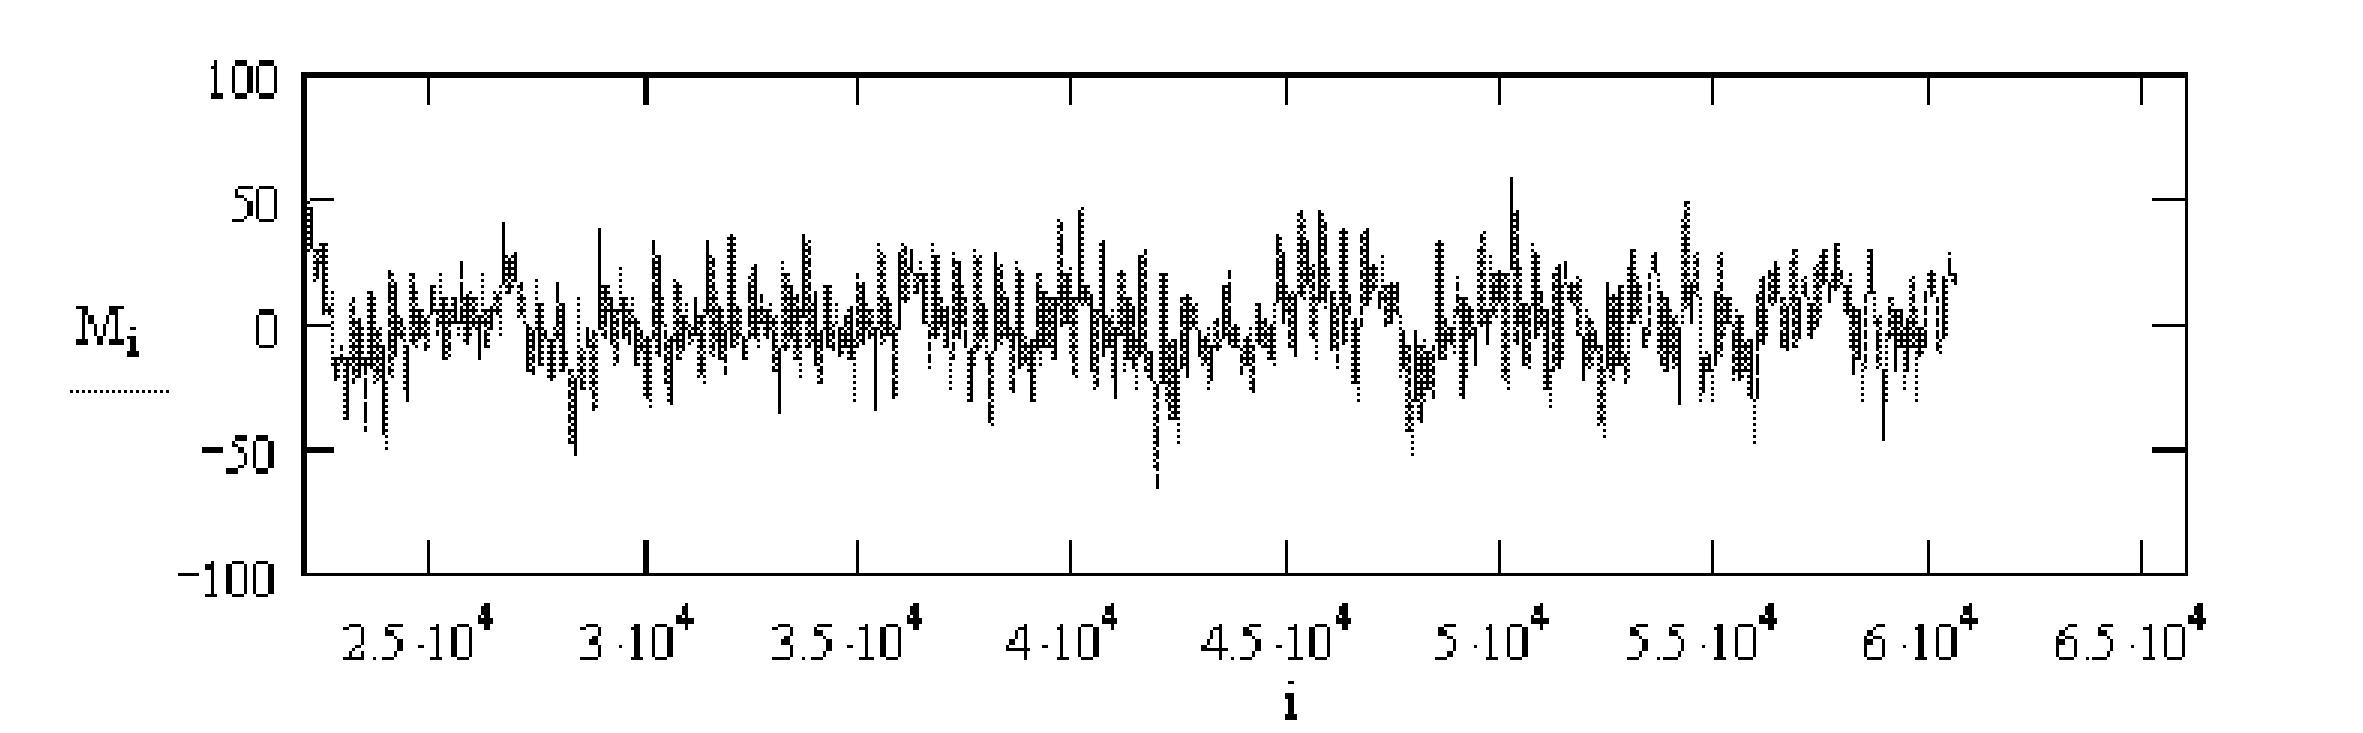
\includegraphics{Images/ReedTime.jpg}  

Recall that we say a function of time g(t) is \textbf{periodic}
(``repeating,'' in our casual wording above) with period T if if g(u+T)
= g(u) for all u. The \textbf{fundamental frequency} of g() is then
defined to be the number of periods per unit time,

\begin{equation}
f_{0}={1\over T}
\end{equation}

Recall also from calculus that we can write a function g(t) (not
necessarily periodic) as a Taylor series, which is an ``infinite
polynomial'':

\begin{equation}
\label{poly}
g(t)=\sum _{n=0}^{\infty }c_{n}t^{n}.
\end{equation}

The specific values of the $c_n$ may be derived by differentiating both
sides of (\ref{poly}) and evaluating at t = 0, yielding 

\begin{equation}
c_n = \frac{g^{(n)}(0)}{n!},
\end{equation}

where $g^{(j)}$ denotes the ith derivative of g().

For instance, for \( e^{t} \),

\begin{equation}
\label{exptaylor}
e^{t}=\sum _{n=0}^{\infty }\frac{1}{n!}t^{n}
\end{equation}

In the case of a repeating function, it is more convenient to use
another kind of series representation, an ``infinite trig polynomial,''
called  a {\bf Fourier series}.  This is just a fancy name for a
weighted sum of sines and cosines of different frequencies.  More
precisely, we can write any repeating function g(t) with period T and
fundamental frequency $f_0$ as    

\begin{equation} 
\label{f2t}
g(t)={\sum _{n=0}^{\infty }{a_{n}}\cos (2\pi nf_{0}t)}+{\sum _{n=1}^{\infty }{b_{n}}\sin (2\pi nf_{0}t)}
\end{equation}

for some set of weights $a_n$ and $b_n$.  Here, instead of having a
weighted sum of terms

\begin{equation}
1,\, \, t,\, \, t^{2},\, \, t^{3},\, \, ...
\end{equation}

as in a Taylor series, we have a weighted sum of terms

\begin{equation}
1,\, \, \cos (2\pi f_{0}t),\, \, \cos (4\pi f_{0}t),\, \, \cos (6\pi f_{0}t),\, \, ...
\end{equation}

and of similar sine terms. Note that the frequencies $nf_0$, in those
sines and cosines are integer multiples of the fundamental frequency of
x, $f_{0}$, called \textbf{harmonics}. 

The weights $a_n$ and $b_n$, n = 0, 1, 2, ... are called the
\textbf{frequency spectrum} of g().  The coefficients are calculated as
follows:\footnote{The get an idea as to how these formulas arise, see
Section \ref{vector}.  But for now, if you integrate both sides of
(\ref{f2t}), you will at least verify that the formulas below do work.}

\begin{equation}
\label{t2fi}
a_{0}=\frac{1}{T}\int _{0}^{T}g(t) ~ dt
\end{equation}

\begin{equation}
\label{t2fii}
a_{n}=\frac{2}{T}\int _{0}^{T}g(t) ~ cos(2\pi nf_{0}t) ~ dt
\end{equation}

\begin{equation}
\label{t2fiii}
b_{n}=\frac{2}{T}\int _{0}^{T}g(t) ~ sin(2\pi nf_{0}t) ~ dt
\end{equation}

By analyzing these weights, we can do things like machine-based voice
recognition (distinguishing one person's voice from another) and speech
recognition (determining what a person is saying).  If for example one
person's voice is higher-pitched than that of another, the first
person's weights will be concentrated more on the
higher-frequency sines and cosines than will the weights of the second.

Since g(t) is a graph of loudness against time, this representation of
the sound is called the {\bf time domain}.  When we find the Fourier
series of the sound, the set of weights $a_n$ and $b_n$ is said to be a
representation of the sound in the {\bf frequency domain}.  One can
recover the original time-domain representation from that of the
frequency domain, and vice versa, as seen in Equations (\ref{t2fi}),
(\ref{t2fii}), (\ref{t2fiii}) and (\ref{f2t}).  

In other words, the transformations between the two domains are inverses
of each other, and there is a one-to-one correspondence between them.
Every g() corresponds to a unique set of weights and vice versa.

Now here is the frequency-domain version of the reed sound:

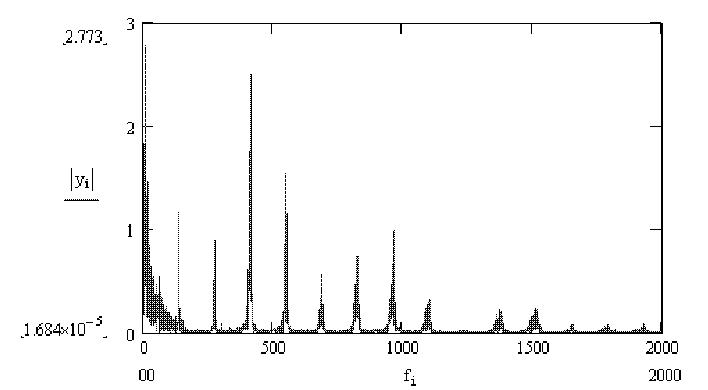
\includegraphics{Images/ReedFreq.jpg}

Note that this graph is very {}``spiky.{}'' In other words, even though
the reed's waveform includes all frequencies, most of the power of the
signal is at a few frequencies which arise from the physical properties
of the reed.   

Fourier series are often expressed in terms of complex numbers, making
use of the relation

\begin{equation}
e^{i \theta} = \cos(\theta) + i ~ \sin(\theta),
\end{equation}

where $i = \sqrt{-1}$.\footnote{There is basically no physical
interpretation of complex numbers.  Instead, they are just
mathematical abstractions.  However, they are highly useful
abstractions, with the complex form of Fourier series, beginning with
(\ref{compact}), being a case in point.

It is not assumed that you know complex variables well.  All that is
required is knowledge of how to add, subtract, multiply and divide, and
the definition of $|c|$ for complex c.}  

The complex form of (\ref{f2t}) is

\begin{equation}
\label{compact}
g(t) = \sum_{j = -\infty}^{\infty} c_j e^{2\pi i j \frac{t}{T}}.
\end{equation}

The $c_j$ are now generally complex numbers.  They are functions of the
$a_j$ and $b_j$, and thus form the frequency spectrum.

Equation (\ref{compact}) has a simpler, more compact form than
(\ref{f2t}).  Do you now see why I referred to Fourier series as trig
polynomials?  The series (\ref{compact}) involves the j$^{th}$ powers of
$e^{2\pi \frac{t}{T} }$.

\subsection{Two-Dimensional Fourier Series}

Let's now move from sounds to images.  Just as we were taking time to be a
continuous variable above, for the time being we are taking the position
within an image to be continuous too; this is equivalent to having
infinitely many pixels.  Here g() is a function of two variables,
g(u,v), where u and v are the horizontal and vertical coordinates of a
point in the image, with g(u,v) being the intensity of the image at that
point.  If it is a gray-scale image, the intensity is whiteness of the
image at that point, typically with 0 being pure black and 255 being
pure white.  If it is a color image, a typical graphics format is to
store three intensity values at a point, one for each of red, green and
blue.  The various colors come from combining three colors at various
intensities.

The terminology changes a bit.  Our original data is now referred to as
being in the {\bf spatial domain}, rather than the time domain. But the
Fourier series coefficients are still said to be in the frequency
domain.

\section{Discrete Fourier Transforms} 
\label{1dim}

In sound and image applications, we seldom if ever know the exact form
of the repeating function g().  All we have is a {\bf sampling} from
g(), i.e. we only have values of g(t) for a set of discrete values of t.

In the sound example above, a typical sampling rate is 8000 samples per
second.\footnote{See Section \ref{sampling} for the reasons behind
this.} So, we may have g(0), g(0.000125), g(0.000250), g(0.000375), and
so on.  In the image case, we sample the image pixel by pixel.

Integrals like (\ref{t2fi}) now change to sums.  

\subsection{One-Dimensional Data}
\label{onedimdft}

Let $X = (x_0,...,x_{n-1})$ denote the sampled values, i.e. the
time-domain representation of g() based on our sample data.  These are
interpreted as data from one period of g(), with the period being n and
the fundamental frequency being 1/n.  The frequency-domain
representation will also consist of n numbers, $c_0,...,c_{n-1}$,
defined as follows:

\begin{equation}
\label{dft}
c_k = 
\frac{1}{n} \sum_{j=0}^{n-1} x_j e^{-2\pi i jk/n} =
\frac{1}{n} \sum_{j=0}^{n-1} x_j q^{jk}
\end{equation}

where

\begin{equation}
q = e^{-2\pi i /n}
\end{equation}

again with $i = \sqrt{-1}$.  The array C of complex numbers $c_k$ is
called the {\bf discrete Fourier transform} (DFT) of X.
Note that (\ref{dft}) is basically a discrete analog of 
(\ref{t2fii}) and (\ref{t2fiii}).

Note that instead of having infinitely many frequencies, we only have n
of them, i.e. the n original data points $x_j$ map to n frequency weights
$c_k$.\footnote{Actually, in the case of $x_j$ real, which occurs with
sound data, we really get only n/2 frequencies.  The weight of the
frequences after k = n/2 turn out to be the {\bf conjugates} of those
before n/2, where the conjugate of a+bi is defined to be a-bi.}

The quantity q is a n$^{th}$ root of 1:

\begin{equation}
q^n = e^{-2 \pi i} = \cos(-2 \pi) + i \sin(-2 \pi) = 1
\end{equation}

Equation (\ref{dft}) can be written as

\begin{equation}
\label{CfromX}
C = \frac{1}{n} A X,
\end{equation}

where X is the vector $x_j$ and 

\begin{equation}
\label{vander}
A = 
\left (
\begin{array}{ccccc}
1 & 1 & 1 & ... & 1 \\
1 & q & q^2 & ... & q^{n-1} \\
... & ... & ... & ... & ... \\
1 & q^{n-1} & q^{2(n-1)} & ... & q^{(n-1)(n-1)}
\end{array}
\right )
\end{equation}

Here's R code to calculate A:

\begin{Verbatim}[fontsize=\relsize{-2},numbers=left]
makeamat <- function(n,u)  {
   m <- matrix(nrow=n,ncol=n)
   for (i in 1:n) {
      for (j in i:n) {
         if (i == j) {
            m[i,i] <- u^((i-1)^2)
         }
         else {
            m[i,j] <- u^((i-1)*(j-1))
            m[j,i] <- m[i,j]
         }
      }
   }
   m
}
\end{Verbatim}

\subsection{Inversion}

As in the continuous case, the DFT is a one-to-one transformation.  so
we can recover each domain from the other.  The details are important:

The matrix A in (\ref{vander}) is a special case of {\bf Vandermonde}
matrices, known to be invertible.  In fact, if we think of that matrix
as a function of q, A(q), then it turns out that

\begin{equation}
\label{vanderinv}
[A(q)]^{-1} = \frac{1}{n} A(\frac{1}{q})
\end{equation}

Thus (\ref{CfromX}) becomes

\begin{equation}
\label{XfromC}
X = n [A(q)]^{-1} C = A(\frac{1}{q}) C
\end{equation}

In nonmatrix terms:

\begin{equation}
\label{dftinv}
x_j = 
\sum_{k=0}^{n-1} c_k e^{2\pi ijk/n}  =
\sum_{k=0}^{n-1} c_k q^{-jk} 
\end{equation}

Equation (\ref{dftinv}) is basically a discrete analog of (\ref{f2t}).

\subsubsection{Alternate Formulation}

Equation (\ref{CfromX}) has a factor 1/n while (\ref{XfromC}) doesn't.
In order to achieve symmetry, some authors of material on DFT opt to
define the DFT and its inverse with $1/\sqrt{n}$ in (\ref{dft}) instead
of 1/n, and by adding a factor $1/\sqrt{n}$ in (\ref{dftinv}).  They
then include a factor $1/\sqrt{n}$ in (\ref{vander}), with the result
that $[A(q)]^{-1} = A(1/q)$.  Thus everything simplifies.  

Other formulations are possible.  For instance, the R {\bf fft()}
routine's documentation says it's ``unnormalized,'' meaning that
there is neither a $1/n$ nor a $1/\sqrt{n}$ in (\ref{dftinv}). 
When using a DFT routine, be sure to determine what it assumes about
these constant factors.

\subsection{Two-Dimensional Data}

The spectrum numbers $c_{rs}$ are double-subscripted, like the original
data $x_{uv}$, the latter being the pixel intensity in row u, column v
of the image, u = 0,1,...,n-1, v = 0,1,...,m-1.  Equation (\ref{dft})
becomes

\begin{equation}
\label{dft2} 
c_{rs} = \frac{1}{n} \frac{1}{m} 
\sum_{j=0}^{n-1} 
\sum_{k=0}^{m-1} 
x_{jk} e^{-2\pi i(\frac{jr}{n}+\frac{ks}{m})}
\end{equation}

where r = 0,1,...,n-1, s = 0,1,...,m-1.

Its inverse is

\begin{equation}
\label{dft2inv}
x_{rs} = 
\sum_{j=0}^{n-1}
\sum_{k=0}^{m-1}
c_{jk} e^{2\pi i(\frac{jr}{n}+\frac{ks}{m})}
\end{equation}

\section{Parallel Computation of Discrete Fourier Transforms}

\subsection{The Fast Fourier Transform}

Speedy computation of a discrete Fourier transform was developed
by Cooley and Tukey in their famous Fast Fourier Transform (FFT), which
takes a ``divide and conquer'' approach:

Equation (\ref{dft}) can be rewritten as

\begin{equation}
c_k = \frac{1}{n} \left [ 
\sum_{j=0}^{m-1} x_{2j} {q}^{2jk} +
\sum_{j=0}^{m-1} x_{2j+1} {q}^{(2j+1)k} ,
\right ] 
\end{equation}

where $m = n/2$. 

After some algebraic manipulation, this becomes

\begin{equation}
\label{recursive} 
c_k = \frac{1}{2} \left [ 
\frac{1}{m} \sum_{j=0}^{m-1} x_{2j} z^{jk} +
q^k \frac{1}{m} \sum_{j=0}^{m-1} x_{2j+1} z^{jk} 
\right ] 
\end{equation}

where $z = e^{-2\pi i/m}$.

A look at Equation (\ref{recursive}) shows that the two sums within the
brackets have the same form as Equation (\ref{dft}).  In other words,
Equation (\ref{recursive}) shows how we can compute an n-point FFT from
two $\frac{n}{2}$-point FFTs.  That means that a DFT can be computed
recursively, cutting the sample size in half at each recursive step. 

In a shared-memory setting such as OpenMP, we could implement this
recursive algorithm in the manners of Quicksort in Chapter
\ref{chap:sort}.  

In a message-passing setting, again because this is a divide-and-conquer
algorithm, we can use the pattern of Hyperquicksort, also in
Chapter \ref{chap:sort}.  

Some digital signal processing chips implement this in hardware, with a
special interconnection network to implement this algorithm.

\subsection{A Matrix Approach}

The matrix form of (\ref{dft}) is

\begin{equation}
\label{matrix}
C = \frac{1}{n} A X
\end{equation}

where A is n x n.  Element (j,k) of A is $q^{jk}$, while
element j of X is $x_j$.  This formulation of the problem then naturally
leads one to use parallel methods for matrix multiplication, as in 
Chapter \ref{chap:matrix}.

Divide-and-conquer tends not to work too well in shared-memory settings,
because after some point, fewer and fewer threads will have work to do.
Thus this matrix formulation is quite valuable.

\subsection{Parallelizing Computation of the Inverse Transform}  

The form of the DFT (\ref{dft}) and its inverse (\ref{dftinv}) are very
similar.  For example, the inverse transform is again of a matrix form
as in (\ref{matrix}); even the new matrix looks a lot like the old 
one.\footnote{In fact, one can obtain the new matrix easily from the
old, as explained in Section \ref{vector}.}

Thus the methods mentioned above, e.g. FFT and the matrix approach,
apply to calculation of the inverse transforms too.

\subsection{Parallelizing Computation of the Two-Dimensional Transform}
\label{par2d}

Regroup (\ref{dft2}) as:

\begin{eqnarray}
\label{dft2new}
c_{rs} &=& 
\frac{1}{n} 
\sum_{j=0}^{n-1}
\left (
\frac{1}{m}
\sum_{k=0}^{m-1}
x_{jk} e^{-2\pi i(\frac{ks}{m})}
\right )
e^{-2\pi i(\frac{jr}{n})} \\
&=&
\label{zzz}
\frac{1}{n}
\sum_{j=0}^{n-1}
y_{js}
e^{-2\pi i(\frac{jr}{n})}
\end{eqnarray}

Note that $y_{js}$, i.e. the expression between the large parentheses,
is the s$^{th}$ component of the DFT of the j$^{th}$ row of our data.
And hey, the last expression (\ref{zzz}) above is in the same form as
(\ref{dft})!  Of course, this means we are taking the DFT of the
spectral coefficients rather than observed data, but numbers are
numbers.  

In other words:  To get the two-dimensional DFT of our data, we first get
the one-dimensional DFTs of each row of the data, place these in rows,
and then find the DFTs of each column.  This property is called {\bf
separability}.

This certainly opens possibilities for parallelization.  Each thread
(shared memory case) or node (message passing case) could handle groups
of rows of the original data, and in the second stage each thread could
handle columns.

Or, we could interchange rows and columns in this process, i.e. put the
j sum inside and k sum outside in the above derivation.

\section{Available FFT Software}

\subsection{R}
\label{rfft}

As of now, R only offers serial computation, through its function {\bf
fft()}.  It works on both one- and two-dimensional (or more) data.  If
its argument {\bf inverse} is set to TRUE, it will find the inverse.

Parallel computation of a two-dimensional transform can be easily
accomplished by using {\bf fft()} together with the approach in Section
\ref{par2d} and one of the packages for parallel R in Chapter
\ref{chap:r}.  Here's how to do it in {\bf snow}:

\begin{lstlisting}[numbers=left]
parfft2 <- function(cls,m) {
   tmp <- parApply(cls,m,1,fft)
   parApply(cls,tmp,1,fft)
}
\end{lstlisting}

Recall that when {\bf parApply()} is called with a vector-valued
function argument, the output from row i of the input matrix is placed
in {\it column} i of the output matrix.  Thus in the second call above,
we used rows (argument 1) instead of columns.

\subsection{CUFFT}

Remember that CUDA includes some excellent FFT routines, in CUFFT.

\subsection{FFTW}

FFTW (``Fastest Fourier Transform in the West'') is available for free
download at \url{http://www.fftw.org}.  It includes versions callable from
OpenMP and MPI.

\section{Applications to Image Processing}

In image processing, there are a number of different operations which we
wish to perform.  We will consider two of them here.

\subsection{Smoothing}
\label{smoothing}

An image may be too ``rough.''  There may be some pixels which are
noise, accidental values that don't fit smoothly with the neighboring
points in the image.

One way to smooth things out would be to replace each pixel intensity
value\footnote{Remember, there may be three intensity values per pixel,
for red, green and blue.} by the mean or median among the pixels
neighbors.  These could be the four immediate neighbors if just a little
smoothing is needed, or we could go further out for a higher amount of
smoothing.  There are many variants of this.

But another way would be to apply a {\bf low-pass filter} to the DFT of
our image.  This means that after we compute the DFT, we simply delete
the higher harmonics, i.e.  set $c_{rs}$ to 0 for the larger values of r
and s.  We then take the inverse transform back to the spatial domain.
Remember, the sine and cosine functions of higher harmonics are
``wigglier,'' so you can see that all this will have the effect 
of removing some of the wiggliness in our image---exactly what we
wanted.

We can control the amount of smoothing by the number of harmonics we
remove.

The term {\it low-pass filter} obviously alludes to the fact that the
low frequencies ``pass'' through the filter but the high frequencies are
blocked.  Since we've removed the high-oscillatory components, the
effect is a smoother image.\footnote{Note that we may do more smoothing
in some parts of the image than in others.}

To do smoothing in parallel, if we just average neighbors, this is
easily parallelized.  If we try a low-pass filter, then we use the
parallelization methods shown here earlier.

\subsection{Example:  Audio Smoothing in R}

Below is code to do smoothing on sound.  It inputs a sound sequence {\bf
snd}, and performs low-pass filtering, setting to 0 all DFT terms having
{\it k} greater than {\tt maxidx} in (\ref{dft}).

\begin{Verbatim}[fontsize=\relsize{-2},numbers=left]
p <- function(snd,maxidx) {
   four <- fft(snd)
   n <- length(four)
   newfour <- c(four[1:maxidx],rep(0,n-maxidx))
   return(Re(fft(newfour,inverse=T)/n))
}
\end{Verbatim}

Here the {\bf Re()} function extracts the real part of a complex number.

\subsection{Edge Detection}

In computer vision applications, we need to have a machine-automated way
to deduce which pixels in an image form an edge of an object.

Again, edge-detection can be done in primitive ways.  Since an edge
is a place in the image in which there is a sharp change in the
intensities at the pixels, we can calculate slopes of the intensities, in
the horizontal and vertical directions.  (This is really calculating the
approximate values of the partial derivatives in those directions.)

But the Fourier approach would be to apply a high-pass filter.  Since an
edge is a set of pixels which are abruptly different from their
neighbors, we want to keep the high-frequency components and block out
the low ones.  

Again, this means first taking the Fourier transform of the original,
then deleting the low-frequency terms, then taking the inverse transform
to go back to the spatial domain.

Below we have ``before and after'' pictures, first of original data 
and then the picture after an edge-detection process has been
applied.\footnote{These pictures are courtesy of Bill Green of
the Robotics Laboratory at Drexel University.  In this case he is
using a Sobel process instead of Fourier analysis, but the result would
have been similar for the latter.  See his Web tutorial at
\url{www.pages.drexel.edu/~weg22/edge.html}, including the original
pictures, which may not show up well in our printed book here.}

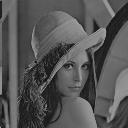
\includegraphics{Images/LENAG.jpg}  

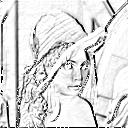
\includegraphics{Images/EDGESOB.jpg}  

The second picture looks like a charcoal sketch!  But it was derived
mathematically from the original picture, using edge-detection methods.

Note that edge detection methods also may be used to determine where
sounds (``ah,'' ``ee'') begin and end in speech-recognition applications.  
In the image case, edge detection is useful for face recognition, etc.

Parallelization here is similar to that of the smoothing case.

\section{R Access to Sound and Image Files}

In order to apply these transformations to sound and image files, you
need to extract the actual data from the files.  The formats are usually
pretty complex.  You can do this easily using the R {\bf tuneR} and {\bf
pixmap} libraries.

After extracting the data, you can apply the transformations, then
transform back to the time/spatial domain, and replace the data
component of the original class.

\section{Keeping the Pixel Intensities in the Proper Range}

Normally pixel intensities are stored as integers between 0 and 255,
inclusive.  With many of the operations mentioned above, both
Fourier-based and otherwise, we can get negative intensity values, or
values higher than 255.  We may wish to discard the negative values and
scale down the positive ones so that most or all are smaller than 256.

Furthermore, even if most or all of our values are in the range 0 to
255, they may be near 0, i.e. too faint.  If so, we may wish to multiply
them by a constant.

\section{Does the Function g() Really Have to Be Repeating?}

It is clear that in the case of a vibrating reed, our loudness function
g(t) really is periodic.  What about other cases?

A graph of your voice would look ``locally periodic."  One difference
would be that the graph would exhibit more change through time as you
make various sounds in speaking, compared to the one repeating sound for
the reed.  Even in this case, though, your voice {\it is} repeating
within short time intervals, each interval corresponding to a different
sound.  If you say the word {\it eye}, for instance, you make an ``ah''
sound and then an ``ee'' sound.  The graph of your voice would show one
repeating pattern during the time you are saying ``ah,'' and another
repeating pattern during the time you are saying ``ee.''  So, even for
voices, we do have repeating patterns over short time intervals.

On the other hand, in the image case, the function may be nearly
constant for long distances (horizontally or vertically), so a local
periodicity argument doesn't seem to work there.

The fact is, though, that it really doesn't matter in the applications
we are considering here.  Even though mathematically our work here has
tacitly assumed that our image is duplicated infinitely times
(horizontally and vertically),\footnote{And in the case of the cosine
transform, implicitly we are assuming that the image flips itself on
every adjacent copy of the image, first right-side up, then upside-own,
then right-side up again, etc.} we don't care about this.  We just want
to get a measure of ``wiggliness,'' and fitting linear combinations of
trig functions does this for us.

\section{Vector Space Issues (optional section)} 
\label{vector}

The theory of Fourier series (and of other similar transforms), relies
on vector spaces.  It actually is helpful to look at some of that here.
Let's first discuss the derivation of (\ref{dft}).  

Define X and C as in Section \ref{1dim}.  X's components are real, but
it is also a member of the vector space V of all n-component arrays of
complex numbers.  

For any complex number a+bi, define its {\bf conjugate},
$\overline{a+bi} = a-bi$.  Note that

\begin{equation}
\overline{e^{i \theta}} = \cos \theta - i \sin \theta = 
= \cos (-\theta) + i \sin (-\theta) =
e^{-i \theta} 
\end{equation}

Define an inner product (``dot product''),

\begin{equation}
[u,w] = \frac{1}{n} \sum_{j=0}^{n-1} u_j \bar{w}_j.
\end{equation}

Define

\begin{equation}
v_h = (1,q^{-h},q^{-2h}, ..., q^{-(n-1)h}), h = 0,1,...,n-1.
\end{equation}

Then it turns out that the $v_h$ form an orthonormal basis for
V.\footnote{Recall that this means that these vectors are orthogonal to
each other, and have length 1, and that they span V.} For example, to
show orthnogonality, observe that for $r \neq s$

\begin{eqnarray}
[v_r,v_s] &=& \frac{1}{n} \sum_{j=0}^{n-1} {v_r}_j \overline{v_s}_j \\
&=& \frac{1}{n} \sum_{j=0} q^{j(-r+s)} \\
&=& \frac{1-q^{(-r+s)n}}{n(1-q)} \\
&=& 0,
\end{eqnarray}

due to the identity  $1+y+y^2+....+y^k = \frac{1-y^{k+1}}{1-y}$ and the
fact that $q^n = 1$.  In the case r = s, the above computation shows
that $[v_r,v_s] = 1$.

The DFT of X, which we called C, can be considered the ``coordinates''
of X in V, relative to this orthonormal basis.  The kth coordinate is
then $[X,v_k]$, which by definition is (\ref{dft}).

The fact that we have an orthonormal basis for V here means that the
matrix A/n in (\ref{matrix}) is an orthogonal matrix.  For real numbers,
this means that this matrix's inverse is its transpose.  In the complex
case, instead of a straight transpose, we do a conjugate transpose,
$B = \overline{A/n}^t$, where t means transpose.  So, B is the inverse of
A/n.  In other words, in (\ref{matrix}), we can easily get back to X
from C, via

\begin{equation}
X = B C = \frac{1}{n} \bar{A}^t C.
\end{equation}

It's really the same for the nondiscrete case.  Here the vector space
consists of all the possible periodic functions g() (with reasonable
conditions placed regarding continuity etc.) forms the vector space, and
the sine and cosine functions form an orthonormal basis.  The $a_n$ and
$b_n$ are then the ``coordinates'' of g() when the latter is viewed as
an element of that space.  

\section{Bandwidth: How to Read the \textit{San Francisco Chronicle}
Business Page (optional section)}
\label{sampling}

The popular press, especially business or technical sections, often
uses the term \textbf{bandwidth}. What does this mean?

Any transmission medium has a natural range $[f_{min} \),\( f_{max}]$
of frequencies that it can handle well. For example, an ordinary
voice-grade telephone line can do a good job of transmitting signals of
frequencies in the range 0 Hz to 4000 Hz, where ``Hz'' means cycles
per second. Signals of frequencies outside this range suffer fade in
strength, i.e are \textbf{attenuated}, as they pass through the phone
line.\footnote{And in fact will probably be deliberately filtered out.}

We call the frequency interval [0,4000] the \textbf{effective
bandwidth} (or just the \textbf{bandwidth}) of the phone line.

In addition to the bandwidth of a \textbf{medium}, we also speak of the
bandwidth of a \textbf{signal}. For instance, although your voice is a
mixture of many different frequencies, represented in the Fourier series
for your voice's waveform, the really low and really high frequency
components, outside the range [340,3400], have very low power, i.e.
their $a_{n}$ and $b_{n}$ coefficients are small. Most of the power of
your voice signal is in that range of frequencies, which we would call
the effective bandwidth of your voice waveform.  This is also the reason
why digitized speech is sampled at the rate of 8,000 samples per second.
A famous theorem, due to Nyquist, shows that the sampling rate should be
double the maximum frequency. Here the number 3,400 is ``rounded up'' to
4,000, and after doubling we get 8,000.

Obviously, in order for your voice to be heard well on the other end
of your phone connection, the bandwidth of the phone line must be
at least as broad as that of your voice signal, and that is the case.

However, the phone line's bandwidth is not much broader than that
of your voice signal. So, some of the frequencies in your voice will
fade out before they reach the other person, and thus some degree
of distortion will occur. It is common, for example, for the letter
`f' spoken on one end to be mis-heard as `s'on the other end. This
also explains why your voice sounds a little different on the phone
than in person. Still, most frequencies are reproduced well and phone
conversations work well.

We often use the term ``bandwidth'' to literally refer to width,
i.e. the width of the interval $[f_{min},f_{max}]$.

There is huge variation in bandwidth among transmission media. As we
have seen, phone lines have bandwidth intervals covering values on the
order of $10^{3}$.  For optical fibers, these numbers are more on the
order of $10^{15}$.  

The radio and TV frequency ranges are large also, which is why, for
example, we can have many AM radio stations in a given city.  The
AM frequency range is divided into subranges, called {\bf channels}.
The width of these channels is on the order of the 4000 we need for a
voice conversation.  That means that the transmitter at a station needs
to shift its content, which is something like in the [0,4000] range, to
its channel range.  It does that by multiplying its content times a sine
wave of frequency equal to the center of the channel.  If one applies a
few trig identities, one finds that the product signal falls into the
proper channel!

Accordingly, an optical fiber could also carry many simultaneous phone
conversations.

Bandwidth also determines how fast we can set digital bits. Think of
sending the sequence 10101010...  If we graph this over time, we get a
``squarewave'' shape.  Since it is repeating, it has a Fourier series.
What happends if we double the bit rate?  We get the same graph, only
horizontally compressed by a factor of two.  The effect of this on this
graph's Fourier series is that, for example, our former $a_3$ will now
be our new $a_6$, i.e. the $2 \pi \cdot 3 f_0$ frequency cosine wave
component of the graph now has the double the old frequency, i.e. is now
$2 \pi \cdot 6 f_0$.  That in turn means that the effective bandwidth of
our 10101010... signal has doubled too.

In other words:  To send high bit rates, we need media with large
bandwidths.



\chapter{Parallel Computation in Statistics/Data Mining}
\label{chap:stat}

How did the word {\it statistics} get supplanted by {\it data mining}?
In a word, it is a matter of scale.

In the old days of statistics, a data set of 300 observations on 3 or 4
variables was considered large.  Today, the widespread use of computers
and the Web yield data sets with numbers of observations that are easily
in the tens of thousands range, and in a number of cases even tens of
millions.  The numbers of variables can also be in the thousands or
more.

In addition, the methods have become much more combinatorial in nature.
In a classification problem, for instance, the old discriminant analysis
involved only matrix computation, whereas a nearest-neighbor analysis
requires far more computer cycles to complete.

In short, this calls for parallel methods of computation.

\section{Itemset Analysis}

\subsection{What Is It?}

The term {\bf data mining} is a buzzword, but all it means is the
process of finding relationships among a set of variables.  In other
words, it would seem to simply be a good old-fashioned statistics
problem.

Well, in fact it {\it is} simply a statistics problem---but writ large,
as mentioned earlier.

{\bf Major, Major Warning:}  With so many variables, the chances of
picking up spurious relations between variables is large.  And although
many books and tutorials on data mining will at least pay lip service to
this issue (referring to it as {\bf overfitting}), they don't emphasize
it enough.\footnote{Some writers recommend splitting one's data into a
{\bf training set}, which is used to discover relationships, and a {\bf
validation set}, which is used to confirm those relationships.  It's a
good idea, but overfitting can still occur even with this precaution.}

Putting the overfitting problem aside, though, by now the reader's
reaction should be, ``This calls for parallel processing,'' and he/she
is correct.  Here we'll look at parallelizing a particular problem,
called {\bf itemset analysis}, the most famous example of which is the
{\bf market basket problem}:

\subsection{The Market Basket Problem}

Consider an online bookstore that has records of every sale on the
store's site.  Those sales may be represented as a matrix S, whose
(i,j)th element $S_{ij}$ is equal to either 1 or 0, depending on whether
the i$^{th}$ sale included book j, i = 0,1,...,s-1, j = 0,1,...,t-1.  So
each row of S represents one sale, with the 1s in that row showing which
titles were bought.  Each column of S represents one book title, with
the 1s showing which sales transactions included that book.

Let's denote the entire line of book titles by $T_0,...,T_{b-1}$.  An
{\bf itemset} is just a subset of this.  A {\bf frequent} itemset is one
which appears in many of sales transactions.  But there is more to it
than that.  The store wants to choose some books for special ads, of the
form ``We see you bought books X and Y.  We think you may be interested
in Z.''

Though we are using marketing as a running example here (which is the
typical way that this subject is introduced), we will usually just refer
to ``items'' instead of books, and to ``database records'' rather than
sales transactions.

We have the following terminology:

\begin{itemize}

\item An {\bf association rule} $I \rightarrow J$ is simply an ordered
pair of disjoint itemsets I and J.

\item The {\bf support} of an an association rule $I \rightarrow J$ is
the proportion of records which include both I and J.

\item The {\bf confidence} of an association rule $I \rightarrow J$ is
the proportion of records which include J, {\it among those records
which include I}.

\end{itemize}

Note that in probability terms, the support is basically P(I and J)
while the confidence is P(J$|$I).  If the confidence is high in the book
example, it means that buyers of the books in set I also tend to buy
those in J.  But this information is not very useful if the support is
low, because it means that the combination occurs so rarely that it may
not be worth our time to deal with it.

So, the user---let's call him/her the ``data miner''---will first set
thresholds for support and confidence, and then set out to find all
association rules for which support and confidence exceed their
respective thresholds.

\subsection{Serial Algorithms}

Various algorithms have been developed to find frequent itemsets and
association rules.  The most famous one for the former task is the {\bf
Apriori} algorithm.  Even it has many forms.  We will discuss one of the
simplest forms here.

The algorithm is basically a breadth-first tree search.  At the root we
find the frequent 1-item itemsets.  In the online bookstore, for
instance, this would mean finding all individual books that appear in at
least r of our sales transaction records, where r is our threshold.

At the second level, we find the frequent 2-item itemsets, e.g. all
pairs of books that appear in at least r sales records, and so on.
After we finish with level i, we then generate new candidate itemsets of
size i+1 from the frequent itemsets we found of size i.

The key point in the latter operation is that if an itemset is not
frequent, i.e. has support less than the threshold, then adding further
items to it will make it even less frequent.  That itemset is then
pruned from the tree, and the branch ends.

Here is the pseudocode:

\begin{tabbing}
set $F_1$ to the set of 1-item itemsets whose support exceeds the
threshold \\
for \=  i = 2 to b \\
  \> $F_{i} = \phi$ \\
  \> for \= each I in $F_{i-1}$ \\
  \> \> for \= each K in $F_1$ \\
  \> \> \> $Q = I \cup K$ \\
  \> \> \> if \= support(Q) exceeds support threshold \\
  \> \> \> \> add Q to $F_{i}$ \\
  \> if $F_{i}$ is empty break \\
return $\cup_i F_i$
\end{tabbing}

In other words, we are building up the itemsets of size i from those of
size i-1, adding all possible choices of one element to each of the
latter.

Again, there are many refinements of this, which shave off work to be
done and thus increase speed.  For example, we should avoid checking the
same itemsets twice, e.g. first \{1,2\} then \{2,1\}.  This can be
accomplished by keeping itemsets in lexicographical order.  We will not
pursue any refinements here.

\subsection{Parallelizing the Apriori Algorithm}

Clearly there is lots of opportunity for parallelizing the serial
algorithm above.  Both of the inner {\bf for} loops can be parallelized
in straightforward ways; they are ``embarrassingly parallel.''  There
are of course critical sections to worry about in the shared-memory
setting, and in the message-passing setting one must designate a manager
node in which to store the $F_i$.

However, as more and more refinements are made in the serial algorithm,
then the parallelism in this algorithm become less and less
``embarrassing.''  And things become more challenging if the storage
needs of the $F_i$, and of their associated ``accounting materials''
such as a directory showing the current tree structure (done via
hash trees), become greater than what can be stored in the memory of one
node, say in the message-passing case.

In other words, parallelizing the market basket problem can be very
challenging.  The interested reader is referred to the considerable
literature which has developed on this topic.

\section{Probability Density Estimation}

Let X denote some quantity of interest in a given population, say
people's heights.  Technically, the {\bf probability density function}
of X, typically denoted by f, is a function on the real line with the
following properties:

\begin{itemize}

\item $f(t) \geq 0$ for all t

\item for any $r < s$,

\begin{equation}
P(r < X < s) = \int_{r}^{s} f(t) ~ dt
\end{equation}

(Note that this implies that f integrates to 1.)

\end{itemize}

This seems abstract, but it's really very simple:  Say we have data on
X, n sample values $X_1,...,X_n$, and we plot a histogram from this
data.  Then {\it f is what the histogram is estimating}.  If we have
more and more data, the histogram gets closer and closer to the true
f.\footnote{The histogram must be scaled to have total area 1.  Most
statistical programs have options for this.}

So, how do we estimate f, and how do we use parallel computing to reduce
the time needed?

\subsection{Kernel-Based Density Estimation}

Histogram computation breaks the real down into intervals, and then
counts how many $X_i$ fall into each interval.  This is fine as a crude
method, but one can do better.

No matter what the interval width is, the histogram will consist of a
bunch of rectanges, rather than a smooth curve.  This problem basically
stems from a lack of weighting on the data.

For example, suppose we are estimating f(25.8), and suppose our
histogram interval is [24.0,26.0], with 54 points falling into that
interval.  Intuitively, we can do better if we give the points closer to
25.8 more weight.

One way to do this is called {\bf kernel-based} density estimation,
which for instance in R is handled by the function {\bf density()}.

We need a set of weights, more precisely a weight function k, called the
{\bf kernel}.  Any nonnegative function which integrates to 1---i.e. a
density function in its own right---will work.  Typically k is taken to
be the Gaussian or normal density function,

\begin{equation}
\label{gaussk}
k(u) = \frac{1}{\sqrt{2 \pi}} e^{-0.5u^2}
\end{equation}

Our estimator is then

\begin{equation}
\label{kernelest}
\widehat{f}(t) = \frac{1}{nh} \sum_{i=1}^{n} k \left ( \frac{t-X_i}{h} \right )
\end{equation}

In statistics, it is customary to use the $\ \widehat{}$ symbol
(pronounced ``hat'') to mean ``estimate of.''  Here $\ \widehat{f}$
means the estimate of f.

Note carefully that we are estimating an entire function!  There are
infinitely many possible values of t, thus infinitely many values of
f(t) to be estimated.  This is reflected in (\ref{kernelest}), as
$\widehat{f}(t)$ does indeed give a (potentially) different value for
each t.

Here h, called the {\it bandwidth}, is playing a role analogous to the
interval width in the case of histograms.  We must choose the value of
h, just like for a histogram we must choose the bin width.\footnote{Some
statistical programs will choose default values, based on theory.}

Again, this looks very abstract, but all it is doing is assigning
weights to the data.  Consider our example above in which we wish to
estimate f(25.8), i.e. t = 25.8 and suppose we choose h to be 6.0.  If
say, $X_{88}$ is 1209.1, very far as away from 25.8, we don't want this
data point to have much weight in our estimation of f(25.8).  Well, it
won't have much weight at all, because the quantity

\begin{equation}
u = \frac{25.8-88}{6}
\end{equation}

will be very large, and (\ref{gaussk}) will be tiny, as u will be way,
way out in the left tail.

Now, keep all this in perspective.  In the end, we will be plotting a
curve, {\it just like we do with a histogram}.  We simply have a more
sophiticated way to do this than plotting a histogram.  Following are
the graphs generated first by the histogram method, then by the kernel
method, on the same data:

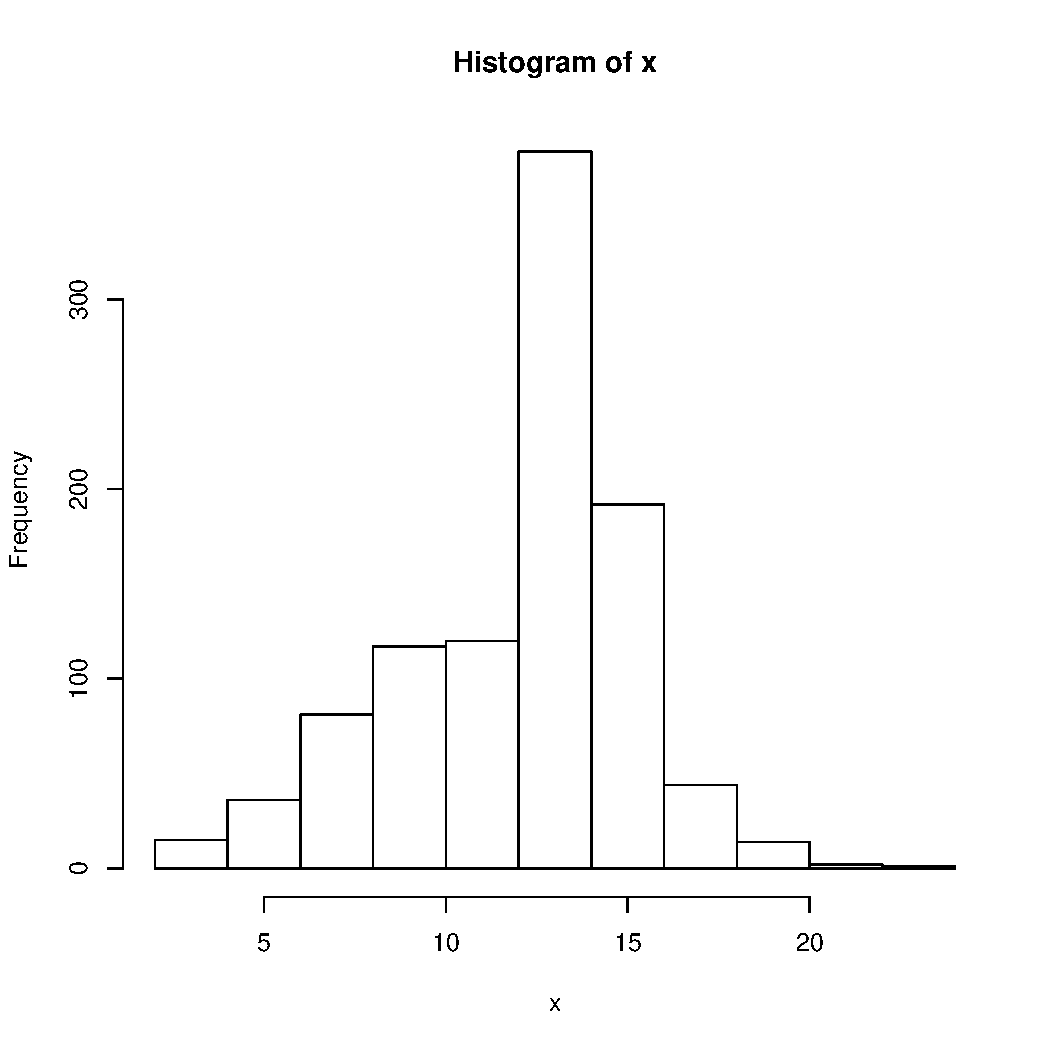
\includegraphics[width=3.0in]{Images/Hist.pdf}

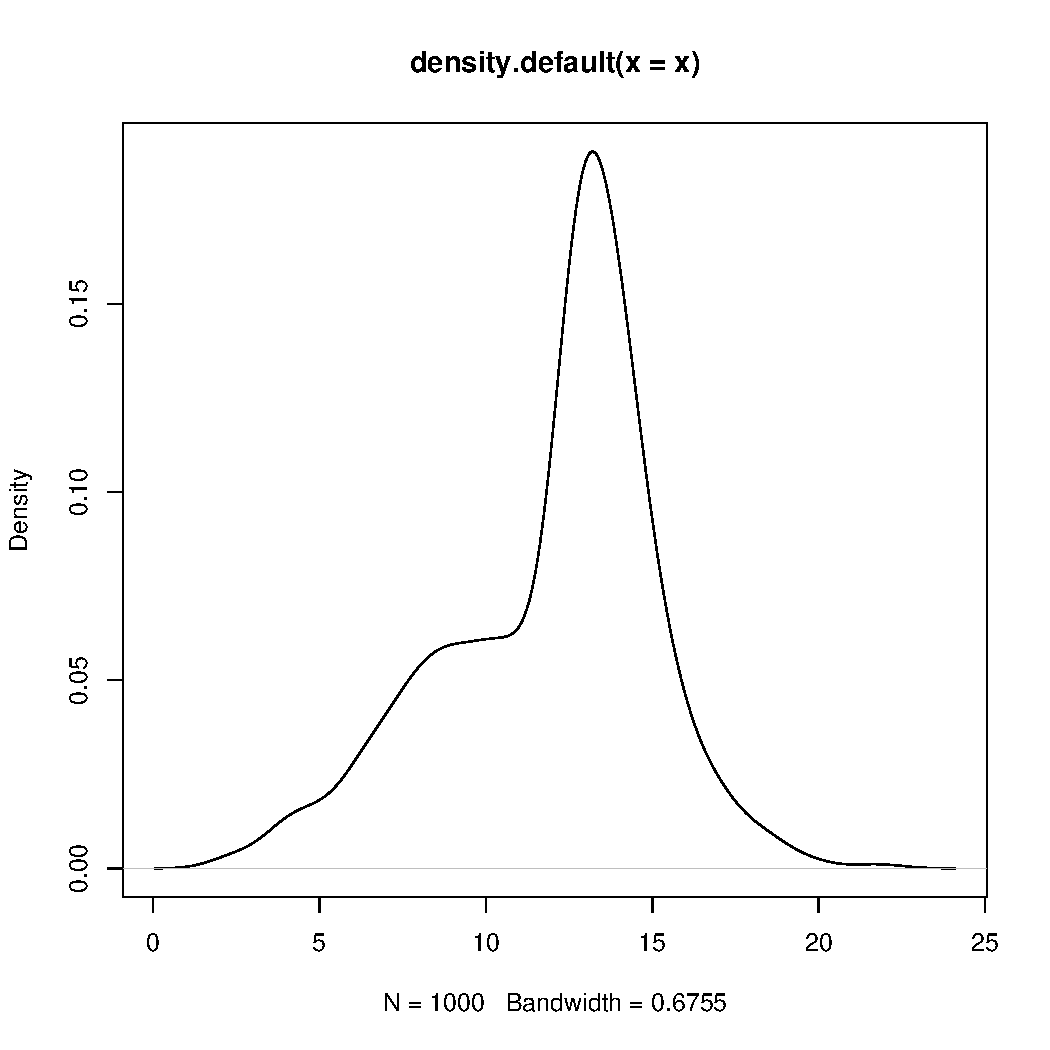
\includegraphics[width=3.0in]{Images/Kern.pdf}

% n <- 1000
% x <- vector(length=n)
% for (i in 1:n) {
%    if (runif(1) < 0.5)  {
%       x[i] <- rnorm(1,mean=10,sd=3)
%    } else x[i] <- rgamma(1,shape=2) + 12
% }
% pdf("Hist.pdf")
% hist(x)
% pdf("Kern.pdf")
% plot(density(x))

There are many ways to parallelize this computation, such as:

\begin{itemize}

\item Remember, we are going to compute (\ref{kernelest}) for many
values of t.  So, we can just have each process compute a block of those
values.

\item We may wish to try several different values of h, just as we might
try several different interval widths for a histogram.  We could have
each process compute using its own values of h.

\item It can be shown that (\ref{kernelest}) has the form of something
called a {\bf convolution}.  The theory of convolution would take us too
far afield,\footnote{

If you've seen the term before and are curious as to how this is a
convolution, read on:

Write (\ref{kernelest}) as

\begin{equation}
\label{kernelesta}
\widehat{f}(t) =
\sum_{i=1}^{n} \frac{1}{h} k \left ( \frac{t-X_i}{h} \right )
   \cdot \frac{1}{n}
\end{equation}

Now consider two artificial random variables U and V, created just for
the purpose of facilitating computation, defined as follows.

The random variable U takes on the values ih with probability $g \cdot
\frac{1}{h} k(i)$, i = -c,-c+1,...,0,1,...,c for some value of c that we
choose to cover most of the area under k, with g chosen so that the
probabilities sum to 1.  The random variable V takes on the values
$X_1,...,X_n$ (considered fixed here), with probability 1/n each.
U and V are set to be independent.

Then (g times) (\ref{kernelesta}) becomes P(U+V=t), exactly what
convolution is about, the probability mass function (or density, in the
continuous case) of a random variable arising as the sum of two
independent nonnegative random variables.} but this fact is useful
here, as the Fourier transform of a convolution can be shown to be the
product of the Fourier transforms of the two convolved
components.\footnote{Again, if you have some background in probability
and have see characteristic functions, this fact comes from the fact
that the characteristic function of the sum of two independent random
variables is equal to the product of the characteristic functions of the
two variables.} In other words, {\it this reduces the problem to that of
parallelizing Fourier transforms}---something we know how to do, from
Chapter \ref{chap:fft}.

\end{itemize}

\subsection{Histogram Computation for Images}

In image processing, histograms are used to find tallies of how many
pixels there are of each intensity.  (Note that there is thus no
interval width issue, as there is a separate ``interval'' value for each
possible intensity level.)  The serial pseudocode is:

\begin{Verbatim}[fontsize=\relsize{-2}]
for i = 1,...,numintenslevels:
   count = 0
   for row = 1,...,numrows:
      for col = 1,...,numcols:
         if image[row][col] == i: count++
   hist[i] = count
\end{Verbatim}

On the surface, this is certainly an ``embarrassingly parallel''
problem.  In OpenMP, for instance, we might have each thread handle a
block of rows of the image, i.e. parallelize the {\bf for row} loop.
In CUDA, we might have each thread handle an individual pixel, thus
parallelizing the nested {\bf for row/col} loops.

However, to make this go fast is a challenge, say in CUDA, due to issues
of what to store in shared memory, when to swap it out, etc.  A very
nice account of fine-tuning this computation in CUDA is given in {\it
Histogram Calculation in CUDA}, by Victor Podlozhnyuk of NVIDIA, 2007,
\url{http://developer.download.nvidia.com/compute/cuda/1_1/Website/projects/histogram256/doc/histogram.pdf}.
The actual code is at
\url{http://developer.download.nvidia.com/compute/cuda/sdk/website/Data-Parallel_Algorithms.html#histogram}.
A summary follows:

%   histogram64:  1-byte counts; BIN_COUNT is 64, for intensity levels
%   0-63 (data is one byte each, so ignore lower 2 bits); chooses 192 as
%   an a middle ground for efficient number of threads, THREAD_N; all
%   threads in a block share a subhistogram, but access different words
%   within it, so don't need; image data is in device global memory; the
%   portion of the subhistogram that a given thread is supposed to
%   accessed are shuffled to avoid bank conflicts; different blocks
%   handle different portions of the image, so subhistograms must be
%   merged; atomicAdd(), if available, is used to write the full
%   histogram, also in device global memory; again shuffling is done

(Much of the research into understand Podlozhnyuk's algorithm was done
by UC Davis graduate student Spencer Mathews.)

Podlozhnyuk's overall plan is to have the threads compute subhistograms
for various chunks of the image, then merge the subhistograms to create
the histogram for the entire data set.  Each thread will handle 1/k of
the image's pixels, where k is the total number of threads in the grid,
i.e. across all blocks.

In Podlozhnyuk's first cut at the problem, he maintains a separate
subhistogram for each thread.  He calls this version of the code {\bf
histogram64}.  The name stems from the fact that only 64 intensity
levels are used, i.e. the more significant 6 bits of each pixel's data
byte.  The reason for this restriction will be discussed later.

Each thread will store its subhistogram as an array of bytes; the count
of pixels that a thread finds to have intensity i will be stored in the
i$^{th}$ byte of this array.  Considering the content of a byte as an
unsigned number, that means that each thread can process only 255
pixels.

The subhistograms will be stored together in a two-dimensional array,
the j$^{th}$ being the subhistogram for thread j.  Since the
subhistograms are accessed repeatedly, we want to store this
two-dimensional array in shared memory.  (Since each pixel will be read
only once, there would be no value in storing it in shared memory, so it
is in global memory.)

The main concern is bank conflicts.  As the various threads in a block
write to the two-dimensional array, they may collide with each other,
i.e. try to write to different locations within the same bank.  But
Podlozhnyuk devised a clever way to stagger the accesses, so that in
fact there are no bank conflicts at all.

In the end, the many subhistograms within a block must be merged, and
those merged counts must in turn be merged across all blocks.  The
former operation is done again by careful ordering to avoid any bank
conflicts, and then the latter is done {\bf atomicAdd()}.

Now, why does {\bf histogram64} tabulate image intensities at only 6-bit
granularity?  It's simply a matter of resource limitations.  Podlozhnyuk
notes that NVIDIA says that for best efficiency, there should be between
128 and 256 threads per block.  He takes the middle ground, 192.  With
16K of shared memory per block, 16K/192 works out to about 85 bytes per
thread.  That eliminates computing a histogram for the full 8-bit image
data, with 256 intensity levels, which would require 256 bytes for each
thread.

Accordingly, Podlozhnyuk offers {\bf histogram256}, which refines the
process, by having one subhistogram per warp, instead of per thread.
This allows the full 8-bit data, 256 levels, to be tabulated, one word
devoted to each count, rather than just one byte.  A subhistogram is now
a table, 256 rows by 32 columns (one column for each thread in the
warp), with each table entry being 4 bytes (1 byte is not sufficient, as
32 threads are tabulating with it).

\section{Clustering}
\label{cluster}

Suppose you have data consisting of (X,Y) pairs, which when plotted look
like this:

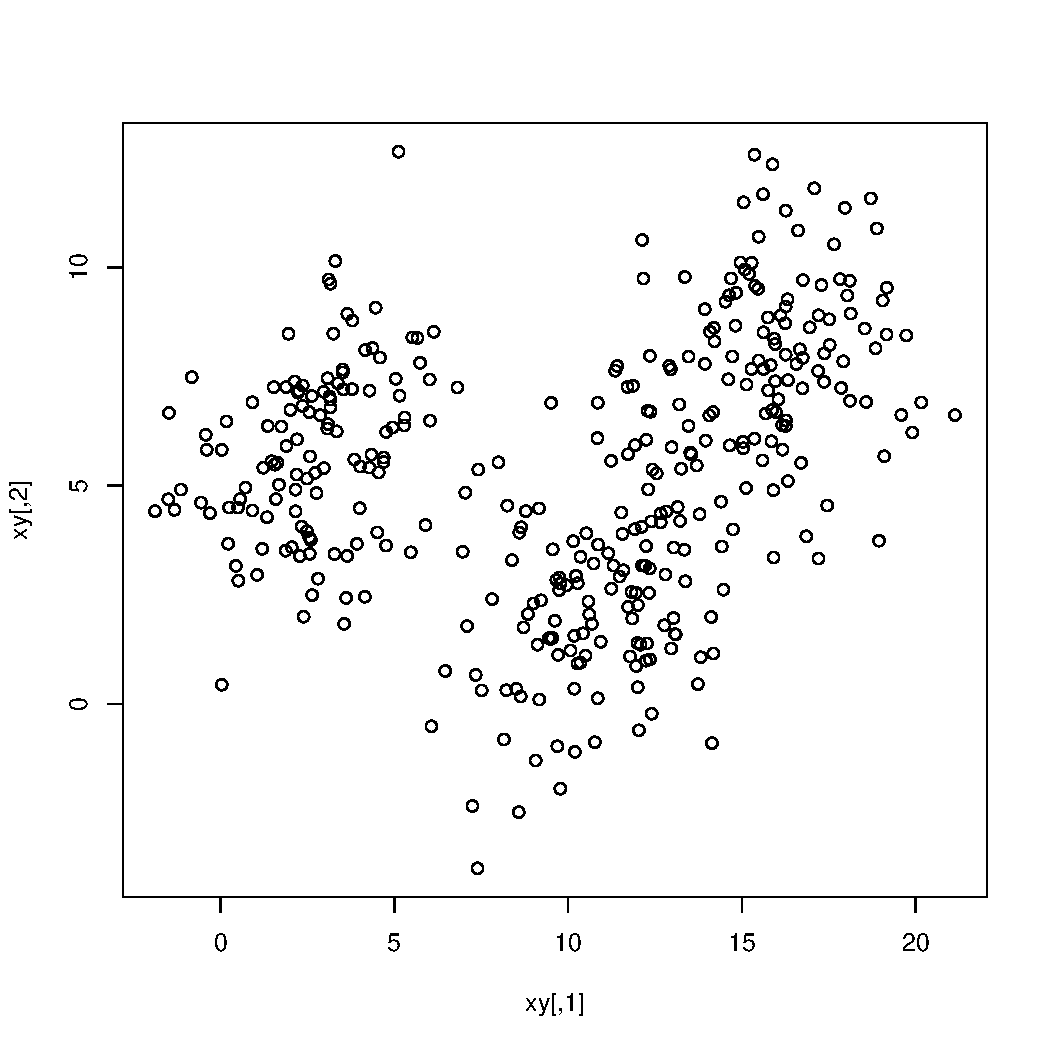
\includegraphics[width=4.0in]{Images/Scatter.pdf}

% library(MASS)
% n <- 125
% xy <- matrix(nrow=3*n,ncol=2)
% sig <- rbind(c(4,1),c(1,4))
% xy[1:n,] <- mvrnorm(n,c(3,6),sig)
% xy[(n+1):(2*n),] <- mvrnorm(n,c(16,8),sig)
% xy[(2*n+1):(3*n),] <- mvrnorm(n,c(11,2),sig)
% # pdf("Scatter.pdf")
% plot(xy)

It looks like there may be two or three groups here.  What clustering
algorithms do is to form groups, both their number and their membership,
i.e. which data points belong to which groups.  (Note carefully that
{\it there is no ``correct'' answer here.  This is merely an exploratory
data analysis tool}.)

Clustering is used is many diverse fields.  For instance, it is used in
image processing for segmentation and edge detection.

Here we have to two variables, say people's heights and weights.  In
general we have many variables, say p of them, so whatever clustering
we find will be in p-dimensional space.  No, we can't picture it very
easily of p is larger than (or even equal to) 3, but we can at least
identify membership, i.e. John and Mary are in group 1, Jenny is in
group 2, etc.  We may derive some insight from this.

There are many, many types of clustering algorithms.  Here we will
discuss the famous {\bf k-means} algorithm, developed by Prof. Jim
MacQueen of the UCLA business school.

The method couldn't be simpler.  Choose k, the number of groups you want
to form, and then run this:

\begin{Verbatim}[fontsize=\relsize{-2},numbers=left]
# form initial groups from the first k data points (or choose randomly)
for i = 1,...,k:
   group[i] = (x[i],y[i])
   center[i] = (x[i],y[i])
do:
   for j = 1,...,n:
      find the closest center[i] to (x[j],y[j])
      cl[j] = the i you got in the previous line
   for i = 1,...,k:
      group[i] = all (x[j],y[j]) such that cl[j] = i
      center[i] = average of all (x,y) in group[i]
until group memberships do not change from one iteration to the next
\end{Verbatim}

Definitions of terms:

\begin{itemize}

\item {\it Closest} means in p-dimensional space, with the usual
Euclidean distance:  The distance from $(a_1,...,a_p$ to $(b_1,...,b_p$
is

\begin{equation}
\sqrt{(b_1-a_1)^2+...+(b_p-a_p)^2}
\end{equation}

Other distance definitions could be used too, of course.

\item The {\it center} of a group is its {\bf centroid}, which is a
fancy name for taking the average value in each component of the data
points in the group.  If p = 2, for example, the center consists of the
point whose X coordinate is the average X value among members of the
group, and whose Y coordinate is the average Y value in the group.

\end{itemize}

\subsection{Example:  k-Means Clustering in R}

In terms of parallelization, again we have an embarrassingly parallel
problem.  Here's {\bf snow} code for it:

\begin{lstlisting}[numbers=left]
# snow version of k-means clustering problem

# returns distances from x to each vector in y;
# here x is a single vector and y is a bunch of them
#
# define distance between 2 points to be the sum of the absolute values
# of their componentwise differences; e.g. distance between (5,4.2) and
# (3,5.6) is 2 + 1.4 = 3.4
dst <- function(x,y) {
   tmpmat <- matrix(abs(x-y),byrow=T,ncol=length(x))  # note recycling
   rowSums(tmpmat)
}

# will check this worker's mchunk matrix against currctrs, the current
# centers of the groups, returning a matrix; row j of the matrix will
# consist of the vector sum of the points in mchunk closest to j-th
# current center, and the count of such points
findnewgrps <- function(currctrs) {
   ngrps <- nrow(currctrs)
   spacedim <- ncol(currctrs)  # what dimension space are we in?
   # set up the return matrix
   sumcounts <- matrix(rep(0,ngrps*(spacedim+1)),nrow=ngrps)
   for (i in 1:nrow(mchunk)) {
      dsts <- dst(mchunk[i,],t(currctrs))
      j <- which.min(dsts)
      sumcounts[j,] <- sumcounts[j,] + c(mchunk[i,],1)
   }
   sumcounts
}

parkm <- function(cls,m,niters,initcenters) {
   n <- nrow(m)
   spacedim <- ncol(m)  # what dimension space are we in?
   # determine which worker gets which chunk of rows of m
   options(warn=-1)
   ichunks <- split(1:n,1:length(cls))
   options(warn=0)
   # form row chunks
   mchunks <- lapply(ichunks,function(ichunk) m[ichunk,])
   mcf <- function(mchunk) mchunk <<- mchunk
   # send row chunks to workers; each chunk will be a global variable at
   # the worker, named mchunk
   invisible(clusterApply(cls,mchunks,mcf))
   # send dst() to workers
   clusterExport(cls,"dst")
   # start iterations
   centers <- initcenters
   for (i in 1:niters) {
      sumcounts <- clusterCall(cls,findnewgrps,centers)
      tmp <- Reduce("+",sumcounts)
      centers <- tmp[,1:spacedim] / tmp[,spacedim+1]
      # if a group is empty, let's set its center to 0s
      centers[is.nan(centers)] <- 0
   }
   centers
}
\end{lstlisting}



\section{Principal Component Analysis (PCA)}
\label{pca}

Consider data consisting of (X,Y) pairs as we saw in Section
\ref{cluster}.  Suppose X and Y are highly correlated with each other.
Then for some constants c and d,

\begin{equation}
\label{onedim}
Y \approx c + d X
\end{equation}

Then in a sense there is really just one random variable here, as the
second is nearly equal to some linear combination of the first.  The
second provides us with almost no new information, once we have the
first.  In other words, even though the vector (X,Y) roams in {\it
two}-dimensional space, it usually sticks close to a {\it
one}-dimensional object, namely the line (\ref{onedim}).

Now think again of p variables.  It may be the case that there exist r
$<$ p variables, consisting of linear combinations of the p variables,
that carry most of the information of the full set of p variables.  If r
is much less than p, we would prefer to work with those r variables.
In data mining, this is called {\bf dimension reduction}.

It can be shown that we can find these r variables by finding the r
eigenvectors corresponding to the r largest eigenvalues of a certain
matrix.  So again we have a matrix formulation, and thus parallelizing
the problem can be done easily by using methods for parallel matrix
operations.  We discussed parallel eigenvector algorithms in Section
\ref{eigen}.

\section{Monte Carlo Simulation}

Monte Carlo simulation is typically (though not always) used to find
probabilistic quantities such as probabilities and expected values.
Consider a simple example problem:

\begin{quote}

An urn contains blue, yellow and green marbles, in numbers 5, 12 and 13,
respectively.  We choose 6 marbles at random.  What is the probability
that we get more yellow marbles than than green and more green than
blue?

\end{quote}

We could find the approximate answer by simulation:

\begin{lstlisting}[numbers=left]
count = 0
for i = 1,...,n
   simulate drawing 6 marbles
   if yellows > greens > blues then count = count + 1
calculate approximate probability as count/n
\end{lstlisting}

The larger n is, the more accurate will be our approximate probability.

At first glance, this problem seems quite embarrassingly parallel.  Say
we are on a shared memory machine running 10 threads and wish to have n
= 100000.  Then we simply have each of our threads run the above code
with n = 10000, and then average our 10 results.

The trouble with this, though, is that it assumes that the random
numbers used by each thread are independent of the others.  A naive
approach, say by calling {\bf random()} in the C library, will not
achieve such independence.  With some random number libraries, in fact,
you'll get the same stream for each thread, certainly not what you want.

A number of techniques have been developed for generating parallel
independent random number streams.  We will not pursue the technical
details here, but will give links to code for them.

\begin{itemize}

\item The NVIDIA CUDA SDK includes a parallel random number
generator, the Mersenne Twister.  The CURAND library has more.

\item RngStream can be used with, for example, OpenMP and MPI.

\item SPRNG is aimed at MPI, but apparently usable in shared memory
settings as well.  Rsprng is an R interface to SPRNG.

\item OpenMP:  An OpenMP version of the Mersenne Twister is available at
\url{http://www.pgroup.com/lit/articles/insider/v2n2a4.htm}.  Other
parallel random number generators for OpenMP are available via a Web
search.

\end{itemize}

There are many, many more.


\chapter{Parallel Python Threads and Multiprocessing Modules} 
\label{chap:pythr}

(Francis Hsu contributed sections of this chapter.)

There are a number of ways to write parallel Python code.\footnote{This 
chapter is shared by two of my open source books:
\url{http://heather.cs.ucdavis.edu/~matloff/158/PLN/ParProcBook.pdf} and
\url{http://heather.cs.ucdavis.edu/~matloff/Python/PLN/FastLanePython.pdf}.
If you wish to more about the topics covered in the book other than the
one you are now reading, please check the other!}

\section{The Python Threads and Multiprocessing Modules}

Python's thread system builds on the underlying OS threads.  They are
thus pre-emptible.  Note, though, that Python adds its own threads
manager on top of the OS thread system; see Section \ref{internals}.

\subsection{Python Threads Modules}

Python threads are accessible via two modules, {\bf thread.py} and {\bf
threading.py}.  The former is more primitive, thus easier to learn from,
and we will start with it.

\subsubsection{The {\tt thread} Module}
\label{threadmodex}

The example here involves a client/server pair.\footnote{It is
preferable here that the reader be familiar with basic network
programming.  See my tutorial at
\url{http://heather.cs.ucdavis.edu/~matloff/Python/PLN/FastLanePython.pdf}.  However,
the comments preceding the various network calls would probably be
enough for a reader without background in networks to follow what is
going on.} As you'll see from reading the comments at the start of the
files, the program does nothing useful, but is a simple illustration of
the principles.  We set up two invocations of the client; they keep
sending letters to the server; the server concatenates all the letters
it receives.

Only the server needs to be threaded.  It will have one thread for each
client.

Here is the client code, {\bf clnt.py}:

\begin{Verbatim}[fontsize=\relsize{-2},numbers=left]
# simple illustration of thread module

# two clients connect to server; each client repeatedly sends a letter,
# stored in the variable k, which the server appends to a global string
# v, and reports v to the client; k = '' means the client is dropping
# out; when all clients are gone, server prints the final string v

# this is the client; usage is

#    python clnt.py server_address port_number

import socket  # networking module
import sys

# create Internet TCP socket
s = socket.socket(socket.AF_INET, socket.SOCK_STREAM)

host = sys.argv[1]  # server address
port = int(sys.argv[2])  # server port

# connect to server
s.connect((host, port))

while(1):
   # get letter
   k = raw_input('enter a letter:')
   s.send(k)  # send k to server
   # if stop signal, then leave loop
   if k == '': break
   v = s.recv(1024)  # receive v from server (up to 1024 bytes)
   print v  

s.close() # close socket
\end{Verbatim}

And here is the server, {\bf srvr.py}:

\begin{Verbatim}[fontsize=\relsize{-2},numbers=left] 
# simple illustration of thread module

# multiple clients connect to server; each client repeatedly sends a
# letter k, which the server adds to a global string v and echos back
# to the client; k = '' means the client is dropping out; when all
# clients are gone, server prints final value of v

# this is the server

import socket  # networking module
import sys

import thread  

# note the globals v and nclnt, and their supporting locks, which are
#    also global; the standard method of communication between threads is
#    via globals

# function for thread to serve a particular client, c
def serveclient(c):
   global v,nclnt,vlock,nclntlock
   while 1:
      # receive letter from c, if it is still connected
      k = c.recv(1)
      if k == '': break
      # concatenate v with k in an atomic manner, i.e. with protection
      #    by locks
      vlock.acquire()
      v += k
      vlock.release()
      # send new v back to client
      c.send(v)
   c.close()
   nclntlock.acquire()
   nclnt -= 1
   nclntlock.release()

# set up Internet TCP socket
lstn = socket.socket(socket.AF_INET, socket.SOCK_STREAM)

port = int(sys.argv[1])  # server port number
# bind lstn socket to this port 
lstn.bind(('', port))
# start listening for contacts from clients (at most 2 at a time)
lstn.listen(5)

# initialize concatenated string, v
v = ''
# set up a lock to guard v
vlock = thread.allocate_lock()  

# nclnt will be the number of clients still connected
nclnt = 2
# set up a lock to guard nclnt
nclntlock = thread.allocate_lock()  

# accept calls from the clients
for i in range(nclnt):
   # wait for call, then get a new socket to use for this client,
   #    and get the client's address/port tuple (though not used)
   (clnt,ap) = lstn.accept()
   # start thread for this client, with serveclient() as the thread's
   #    function, with parameter clnt; note that parameter set must be
   #    a tuple; in this case, the tuple is of length 1, so a comma is
   #    needed
   thread.start_new_thread(serveclient,(clnt,))

# shut down the server socket, since it's not needed anymore 
lstn.close()

# wait for both threads to finish 
while nclnt > 0: pass

print 'the final value of v is', v
\end{Verbatim}

Make absolutely sure to run the programs before proceeding
further.\footnote{You can get them from the {\bf .tex} source file for
this tutorial, located wherever your picked up the {\bf .pdf} version.}
Here is how to do this:  

I'll refer to the machine on which you run the server as {\bf a.b.c},
and the two client machines as {\bf u.v.w} and {\bf x.y.z}.\footnote{You
could in fact run all of them on the same machine, with address name
{\bf localhost} or something like that, but it would be better on
separate machines.}  First, on the server machine, type

\begin{verbatim}
python srvr.py 2000
\end{verbatim}

and then on each of the client machines type

\begin{verbatim}
python clnt.py a.b.c 2000
\end{verbatim}

(You may need to try another port than 2000, anything above 1023.)

Input letters into both clients, in a rather random pattern, typing some
on one client, then on the other, then on the first, etc.  Then finally
hit Enter without typing a letter to one of the clients to end the
session for that client, type a few more characters in the other client,
and then end that session too.

The reason for threading the server is that the inputs from the clients
will come in at unpredictable times.  At any given time, the server
doesn't know which client will send input next, and thus doesn't know on
which client to call {\bf recv()}.  One way to solve this problem is by
having threads, which run ``simultaneously'' and thus give the server
the ability to read from whichever client has sent data.\footnote{Another 
solution is to use nonblocking I/O.  See this example in that context in
\url{http://heather.cs.ucdavis.edu/~matloff/Python/PyNet.pdf}}.  

So, let's see the technical details.  We start with the ``main''
program.\footnote{Just as you should write the main program first, you
should read it first too, for the same reasons.}

\begin{Verbatim}[fontsize=\relsize{-2}]
vlock = thread.allocate_lock()  
\end{Verbatim}

Here we set up a {\bf lock variable} which guards {\bf
v}.  We will explain later why this is needed.  Note that in order to
use this function and others we needed to import the {\bf thread}
module.

\begin{Verbatim}[fontsize=\relsize{-2}]
nclnt = 2
nclntlock = thread.allocate_lock()  
\end{Verbatim}

We will need a mechanism to insure that the ``main'' program, which also
counts as a thread, will be passive until both application threads have
finished.  The variable {\bf nclnt} will serve this purpose.  It will be
a count of how many clients are still connected.  The ``main'' program
will monitor this, and wrap things up later when the count reaches 0. 

\begin{Verbatim}[fontsize=\relsize{-2}]
thread.start_new_thread(serveclient,(clnt,))
\end{Verbatim}

Having accepted a a client connection, the server sets up a thread for
serving it, via {\bf thread.start\_new\_thread()}.  The first argument
is the name of the application function which the thread will run, in
this case {\bf serveclient()}.  The second argument is a tuple
consisting of the set of arguments for that application function.  As
noted in the comment, this set is expressed as a tuple, and since in
this case our tuple has only one component, we use a comma to signal the
Python interpreter that this is a tuple.

So, here we are telling Python's threads system to call our function
{\bf serveclient()}, supplying that function with the argument {\bf
clnt}.  The thread becomes ``active'' immediately, but this does not
mean that it starts executing right away.  All that happens is that the
threads manager adds this new thread to its list of threads, and marks
its current state as Run, as opposed to being in a Sleep state, waiting
for some event. 

By the way, this gives us a chance to show how clean and elegant
Python's threads interface is compared to what one would need in C/C++.
For example, in {\bf pthreads}, the function analogous to 
{\bf thread.start\_new\_thread()} has the signature

\begin{Verbatim}[fontsize=\relsize{-2}]
pthread_create (pthread_t *thread_id, const pthread_attr_t *attributes,
   void *(*thread_function)(void *), void *arguments);
\end{Verbatim}

What a mess!  For instance, look at the types in that third argument:  A
pointer to a function whose argument is pointer to {\tt void} and whose
value is a pointer to {\tt void} (all of which would have to be {\tt
cast} when called).  It's such a pleasure to work in Python, where we
don't have to be bothered by low-level things like that.

Now consider our statement

\begin{Verbatim}[fontsize=\relsize{-2}]
while nclnt > 0: pass
\end{Verbatim}

The statement says that as long as at least one client is still active,
do nothing.  Sounds simple, and it is, but you should consider what is
really happening here.

Remember, the three threads---the two client threads, and the ``main''
one---will take turns executing, with each turn lasting a brief period
of time.  Each time ``main'' gets a turn, it will loop repeatedly on
this line.  But all that empty looping in ``main'' is wasted time.  What
we would really like is a way to prevent the ``main'' function from
getting a turn at all until the two clients are gone.  There are ways to
do this which you will see later, but we have chosen to remain simple
for now.

Now consider the function {\bf serveclient()}.  Any thread executing
this function will deal with only one particular client, the one
corresponding to the connection {\bf c} (an argument to the function).
So this {\bf while} loop does nothing but read from that particular
client.  If the client has not sent anything, the thread will block on 
the line

\begin{Verbatim}[fontsize=\relsize{-2}]
k = c.recv(1)
\end{Verbatim}

This thread will then be marked as being in Sleep state by the thread
manager, thus allowing the other client thread a chance to run.  If
neither client thread can run, then the ``main'' thread keeps getting
turns.  When a user at one of the clients finally types a letter, the
corresponding thread unblocks, i.e. the threads manager changes its
state to Run, so that it will soon resume execution.

Next comes the most important code for the purpose of this tutorial:

\begin{Verbatim}[fontsize=\relsize{-2}]
vlock.acquire()
v += k
vlock.release()
\end{Verbatim}

Here we are worried about a {\bf race condition}.  Suppose for example
{\bf v} is currently 'abx', and Client 0 sends {\bf k} equal to 'g'.
The concern is that this thread's turn might end in the middle of that
addition to {\bf v}, say right after the Python interpreter had formed
'abxg' but before that value was written back to {\bf v}.  This could be
a big problem.  The next thread might get to the same statement, take
{\bf v}, still equal to 'abx', and append, say, 'w', making {\bf v}
equal to 'abxw'.  Then when the first thread gets its next turn, it
would finish its interrupted action, and set {\bf v} to 'abxg'---which
would mean that the 'w' from the other thread would be lost.  

All of this hinges on whether the operation

\begin{Verbatim}[fontsize=\relsize{-2}]
v += k
\end{Verbatim}

is interruptible.  Could a thread's turn end somewhere in the midst of
the execution of this statement?  If not, we say that the operation is
{\bf atomic}.  If the operation were atomic, we would not need the
lock/unlock operations surrounding the above statement.  I did this,
using the methods described in Section \ref{gil}, and it appears to me
that the above statement is {\it not} atomic.

Moreover, it's safer not to take a chance, especially since Python
compilers could vary or the virtual machine could change; after all, we
would like our Python source code to work even if the machine changes.

So, we need the lock/unlock operations:

\begin{Verbatim}[fontsize=\relsize{-2}]
vlock.acquire()
v += k
vlock.release()
\end{Verbatim}

The lock, {\bf vlock} here, can only be held by one thread at a time.
When a thread executes this statement, the Python interpreter will check
to see whether the lock is locked or unlocked right now.  In the latter
case, the interpreter will lock the lock and the thread will continue,
and will execute the statement which updates {\bf v}.  It will then
release the lock, i.e. the lock will go back to unlocked state.

If on the other hand, when a thread executes {\bf acquire()} on this
lock when it is locked, i.e. held by some other thread, its turn will
end and the interpreter will mark this thread as being in Sleep state,
waiting for the lock to be unlocked.  When whichever thread currently
holds the lock unlocks it, the interpreter will change the blocked
thread from Sleep state to Run state.

Note that if our threads were non-preemptive, we would not need
these locks.

Note also the crucial role being played by the global nature of {\bf v}.
Global variables are used to communicate between threads.  In fact,
recall that this is one of the reasons that threads are so
popular---easy access to global variables.  Thus the dogma so often
taught in beginning programming courses that global variables must be
avoided is wrong; on the contrary, there are many situations in which
globals are necessary and natural.\footnote{I think that dogma is
presented in a far too extreme manner anyway.  See
\url{http://heather.cs.ucdavis.edu/~matloff/globals.html}. }

The same race-condition issues apply to the code

\begin{Verbatim}[fontsize=\relsize{-2}]
nclntlock.acquire()
nclnt -= 1
nclntlock.release()
\end{Verbatim}

Following is a Python program that finds prime numbers using threads.
Note carefully that it is not claimed to be efficient at all (it may
well run more slowly than a serial version); it is merely an
illustration of the concepts.  Note too that we are again using the
simple {\bf thread} module, rather than {\bf threading}.

\begin{Verbatim}[fontsize=\relsize{-2},numbers=left]
#!/usr/bin/env python

import sys
import math
import thread

def dowork(tn):  # thread number tn
   global n,prime,nexti,nextilock,nstarted,nstartedlock,donelock
   donelock[tn].acquire()
   nstartedlock.acquire()
   nstarted += 1
   nstartedlock.release()
   lim = math.sqrt(n)
   nk = 0
   while 1:
      nextilock.acquire()
      k = nexti
      nexti += 1
      nextilock.release()
      if k > lim: break
      nk += 1
      if prime[k]:
         r = n / k
         for i in range(2,r+1):
            prime[i*k] = 0
   print 'thread', tn, 'exiting; processed', nk, 'values of k'
   donelock[tn].release()

def main():
   global n,prime,nexti,nextilock,nstarted,nstartedlock,donelock
   n = int(sys.argv[1])
   prime = (n+1) * [1]
   nthreads = int(sys.argv[2])
   nstarted = 0
   nexti = 2
   nextilock = thread.allocate_lock()  
   nstartedlock = thread.allocate_lock()  
   donelock = []
   for i in range(nthreads):
      d = thread.allocate_lock()  
      donelock.append(d) 
      thread.start_new_thread(dowork,(i,))
   while nstarted < nthreads: pass
   for i in range(nthreads):
      donelock[i].acquire()  
   print 'there are', reduce(lambda x,y: x+y, prime) - 2, 'primes'

if __name__ == '__main__':
    main()
\end{Verbatim}

So, let's see how the code works.

The algorithm is the famous Sieve of Erathosthenes:  We list all the
numbers from 2 to {\bf n}, then cross out all multiples of 2 (except 2),
then cross out all multiples of 3 (except 3), and so on.  The numbers
which get crossed out are composite, so the ones which remain at the end
are prime.

{\bf Line 32:}  We set up an array {\bf prime}, which is what we will be
``crossing out.''  The value 1 means ``not crossed out,'' so we start
everything at 1.  (Note how Python makes this easy to do, using list
``multiplication.'')

{\bf Line 33:}  Here we get the number of desired threads from the
command line.

{\bf Line 34:}  The variable {\bf nstarted} will show how many threads
have already started.  This will be used later, in Lines 43-45, in
determining when the {\bf main()} thread exits.  Since the various
threads will be writing this variable, we need to protect it with a
lock, on Line 37.

{\bf Lines 35-36:}  The variable {\bf nexti} will say which value we
should do ``crossing out'' by next.  If this is, say, 17, then it means
our next task is to cross out all multiples of 17 (except 17).  Again we
need to protect it with a lock.

{\bf Lines 39-42:}  We create the threads here.  The function executed
by the threads is named {\bf dowork()}.  We also create locks in an
array {\bf donelock}, which again will be used later on as a mechanism
for determining when {\bf main()} exits (Line 44-45).

{\bf Lines 43-45:}  There is a lot to discuss here.  

To start, recall that in {\bf srvr.py}, our example in Section
\ref{threadmodex}, we didn't want the main thread to exit until the
child threads were done.\footnote{The effect of the main thread ending
earlier would depend on the underlying OS.  On some platforms, exit of
the parent may terminate the child threads, but on other platforms the
children continue on their own.}  So, Line 50 was a {\bf busy wait},
repeatedly doing nothing ({\bf pass}).  That's a waste of time---each
time the main thread gets a turn to run, it repeatedly executes {\bf
pass} until its turn is over.

Here in our primes program, a premature exit by {\bf main()} result in
printing out wrong answers.  On the other hand, we don't want {\bf
main()} to engage in a wasteful busy wait.  We could use {\bf join()} 
from {\bf threading.Thread} for this purpose, to be discussed later, but
here we take a different tack:  We set up a list of locks, one for each
thread, in a list {\bf donelock}.  Each thread initially acquires its
lock (Line 9), and releases it when the thread finishes its work (Lin
27).  Meanwhile, {\bf main()} has been waiting to acquire those locks
(Line 45).  So, when the threads finish, {\bf main()} will move on to
Line 46 and print out the program's results.

But there is a subtle problem (threaded programming is notorious for
subtle problems), in that there is no guarantee that a thread will
execute Line 9 before {\bf main()} executes Line 45.  That's why we have
a busy wait in Line 43, to make sure all the threads acquire their locks
before {\bf main()} does.  Of course, we're trying to avoid busy waits,
but this one is quick.

{\bf Line 13:}  We need not check any ``crosser-outers'' that are larger
than $\sqrt{n}$.  

{\bf Lines 15-25:}  We keep trying ``crosser-outers'' until we reach
that limit (Line 20).  Note the need to use the lock in Lines 16-19.
In Line 22, we check the potential ``crosser-outer'' for primeness; if
we have previously crossed it out, we would just be doing duplicate work
if we used this {\bf k} as a ``crosser-outer.''

Here's one more example, a type of Web crawler.  This one continually
monitors the access time of the Web, by repeatedly accessing a list of
``representative'' Web sites, say the top 100.  What's really different
about this program, though, is that we've reserved one thread for human
interaction.  The person can, whenever he/she desires, find for instance
the mean of recent access times.

\begin{Verbatim}[fontsize=\relsize{-2},numbers=left]
import sys
import time
import os
import thread

class glbls:
   acctimes = []  # access times
   acclock = thread.allocate_lock()  # lock to guard access time data
   nextprobe = 0  # index of next site to probe
   nextprobelock = thread.allocate_lock()  # lock to guard access time data
   sites = open(sys.argv[1]).readlines()  # the sites to monitor
   ww = int(sys.argv[2])  # window width

def probe(me):
   if me > 0:
      while 1:
         # determine what site to probe next
         glbls.nextprobelock.acquire()
         i = glbls.nextprobe
         i1 = i + 1
         if i1 >= len(glbls.sites): i1 = 0
         glbls.nextprobe = i1
         glbls.nextprobelock.release()
         # do probe
         t1 = time.time()
         os.system('wget --spider -q '+glbls.sites[i1])
         t2 = time.time()
         accesstime = t2 - t1  
         glbls.acclock.acquire()
         # list full yet?
         if len(glbls.acctimes) < glbls.ww:
            glbls.acctimes.append(accesstime)
         else:
            glbls.acctimes = glbls.acctimes[1:] + [accesstime]
         glbls.acclock.release()
   else:
      while 1:
         rsp = raw_input('monitor: ')
         if rsp == 'mean': print mean(glbls.acctimes)
         elif rsp == 'median': print median(glbls.acctimes)
         elif rsp == 'all': print all(glbls.acctimes)

def mean(x):
   return sum(x)/len(x)

def median(x):
   y = x
   y.sort()
   return y[len(y)/2]  # a little sloppy

def all(x):
   return x

def main():
   nthr = int(sys.argv[3])  # number of threads
   for thr in range(nthr):
      thread.start_new_thread(probe,(thr,))
   while 1: continue

if __name__ == '__main__': 
   main() 

\end{Verbatim}

\subsubsection{The {\tt threading} Module}  
\label{threadingmodex}

The program below treats the same network client/server application
considered in Section \ref{threadmodex}, but with the more sophisticated
{\bf threading} module.  The client program stays the same, since it
didn't involve threads in the first place.  Here is the new server code:

\begin{Verbatim}[fontsize=\relsize{-2},numbers=left]
# simple illustration of threading module

# multiple clients connect to server; each client repeatedly sends a
# value k, which the server adds to a global string v and echos back
# to the client; k = '' means the client is dropping out; when all
# clients are gone, server prints final value of v

# this is the server

import socket  # networking module
import sys
import threading 

# class for threads, subclassed from threading.Thread class 
class srvr(threading.Thread):
   # v and vlock are now class variables
   v = ''
   vlock = threading.Lock()
   id = 0  # I want to give an ID number to each thread, starting at 0
   def __init__(self,clntsock):
      # invoke constructor of parent class
      threading.Thread.__init__(self)
      # add instance variables
      self.myid = srvr.id
      srvr.id += 1
      self.myclntsock = clntsock 
   # this function is what the thread actually runs; the required name
   #    is run(); threading.Thread.start() calls threading.Thread.run(),
   #    which is always overridden, as we are doing here
   def run(self):
      while 1:
         # receive letter from client, if it is still connected
         k = self.myclntsock.recv(1)
         if k == '': break
         # update v in an atomic manner
         srvr.vlock.acquire()
         srvr.v += k
         srvr.vlock.release()
         # send new v back to client
         self.myclntsock.send(srvr.v)
      self.myclntsock.close()

# set up Internet TCP socket
lstn = socket.socket(socket.AF_INET, socket.SOCK_STREAM)
port = int(sys.argv[1])  # server port number
# bind lstn socket to this port 
lstn.bind(('', port))
# start listening for contacts from clients (at most 2 at a time)
lstn.listen(5)

nclnt = int(sys.argv[2])  # number of clients

mythreads = []  # list of all the threads
# accept calls from the clients
for i in range(nclnt):
   # wait for call, then get a new socket to use for this client,
   #    and get the client's address/port tuple (though not used)
   (clnt,ap) = lstn.accept()
   # make a new instance of the class srvr 
   s = srvr(clnt)
   # keep a list all threads
   mythreads.append(s)
   # threading.Thread.start calls threading.Thread.run(), which we
   #    overrode in our definition of the class srvr
   s.start()

# shut down the server socket, since it's not needed anymore 
lstn.close()

# wait for all threads to finish 
for s in mythreads:
   s.join()

print 'the final value of v is', srvr.v
\end{Verbatim}

Again, let's look at the main data structure first:

\begin{Verbatim}[fontsize=\relsize{-2}]
class srvr(threading.Thread):
\end{Verbatim}

The {\bf threading} module contains a class {\bf Thread}, any instance
of which represents one thread.  A typical application will subclass
this class, for two reasons.  First, we will probably have some
application-specific variables or methods to be used.  Second, the class
{\bf Thread} has a member method {\bf run()} which is meant to be
overridden, as you will see below.

Consistent with OOP philosophy, we might as well put the old globals in
as class variables:

\begin{Verbatim}[fontsize=\relsize{-2}]
v = ''
vlock = threading.Lock()
\end{Verbatim}

Note that class variable code is executed immediately upon execution of the
program, as opposed to when the first object of this class is created.
So, the lock is created right away.

\begin{Verbatim}[fontsize=\relsize{-2}]
id = 0
\end{Verbatim}

This is to set up ID numbers for each of the threads.  We don't use them
here, but they might be useful in debugging or in future enhancement of
the code.

\begin{Verbatim}[fontsize=\relsize{-2}]
def __init__(self,clntsock):
   ...
   self.myclntsock = clntsock

# ``main'' program
...
   (clnt,ap) = lstn.accept()
   s = srvr(clnt)
\end{Verbatim}

The ``main'' program, in creating an object of this class for the
client, will pass as an argument the socket for that client.  We then
store it as a member variable for the object.

\begin{Verbatim}[fontsize=\relsize{-2}]
def run(self):
   ...
\end{Verbatim}

As noted earlier, the {\bf Thread} class contains a member method {\bf
run()}.  This is a dummy, to be overridden with the application-specific
function to be run by the thread.  It is invoked by the method {\bf
Thread.start()}, called here in the main program.  As you can see above,
it is pretty much the same as the previous code in Section
\ref{threadmodex} which used the {\bf thread} module, adapted to the
class environment.

One thing that is quite different in this program is the way we end
it:

\begin{Verbatim}[fontsize=\relsize{-2}]
for s in mythreads:
   s.join()
\end{Verbatim}

The {\bf join()} method in the class {\bf Thread} blocks until the given
thread exits.  (The threads manager puts the main thread in Sleep state,
and when the given thread exits, the manager changes that state to Run.)
The overall effect of this loop, then, is that the main program will
wait at that point until all the threads are done.  They ``join'' the
main program.  This is a much cleaner approach than what we used
earlier, and it is also more efficient, since the main program will not
be given any turns in which it wastes time looping around doing nothing,
as in the program in Section \ref{threadmodex} in the line

\begin{Verbatim}[fontsize=\relsize{-2}]
while nclnt > 0: pass
\end{Verbatim}

Here we maintained our own list of threads.  However, we could also get
one via the call {\bf threading.enumerate()}.  If placed after the {\bf
for} loop in our server code above, for instance as

\begin{Verbatim}[fontsize=\relsize{-2}]
print threading.enumerate()
\end{Verbatim}

we would get output like

\begin{Verbatim}[fontsize=\relsize{-2}]
[<_MainThread(MainThread, started)>, <srvr(Thread-1, started)>,
<srvr(Thread-2, started)>]
\end{Verbatim}

Here's another example, which finds and counts prime numbers, again not
assumed to be efficient:

\begin{Verbatim}[fontsize=\relsize{-2},numbers=left]
#!/usr/bin/env python

# prime number counter, based on Python threading class

# usage:  python PrimeThreading.py n nthreads 
#   where we wish the count of the number of primes from 2 to n, and to
#   use nthreads to do the work

# uses Sieve of Erathosthenes:  write out all numbers from 2 to n, then
# cross out all the multiples of 2, then of 3, then of 5, etc., up to
# sqrt(n); what's left at the end are the primes

import sys
import math
import threading

class prmfinder(threading.Thread):
   n = int(sys.argv[1])
   nthreads = int(sys.argv[2])
   thrdlist = []  # list of all instances of this class
   prime = (n+1) * [1]  # 1 means assumed prime, until find otherwise
   nextk = 2  # next value to try crossing out with
   nextklock = threading.Lock()
   def __init__(self,id):
      threading.Thread.__init__(self)
      self.myid = id
   def run(self):
      lim = math.sqrt(prmfinder.n)
      nk = 0  # count of k's done by this thread, to assess load balance
      while 1:
         # find next value to cross out with
         prmfinder.nextklock.acquire()
         k = prmfinder.nextk
         prmfinder.nextk += 1
         prmfinder.nextklock.release()
         if k > lim: break
         nk += 1  # increment workload data
         if prmfinder.prime[k]:  # now cross out
            r = prmfinder.n / k
            for i in range(2,r+1):
               prmfinder.prime[i*k] = 0
      print 'thread', self.myid, 'exiting; processed', nk, 'values of k'

def main():
   for i in range(prmfinder.nthreads):
      pf = prmfinder(i)  # create thread i
      prmfinder.thrdlist.append(pf) 
      pf.start()
   for thrd in prmfinder.thrdlist: thrd.join()
   print 'there are', reduce(lambda x,y: x+y, prmfinder.prime) - 2, 'primes'

if __name__ == '__main__':
    main()
\end{Verbatim}

\subsection{Condition Variables}

\subsubsection{General Ideas}

We saw in the last section that {\bf threading.Thread.join()} avoids the
need for wasteful looping in {\bf main()}, while the latter is waiting
for the other threads to finish.  In fact, it is very common in threaded
programs to have situations in which one thread needs to wait for
something to occur in another thread.  Again, in such situations we
would not want the waiting thread to engage in wasteful looping.

The solution to this problem is {\bf condition variables}.  As the name
implies, these are variables used by code to wait for a certain
condition to occur.  Most threads systems include provisions for these,
and Python's {\bf threading} package is no exception.  

The {\bf pthreads} package, for instance, has a type {\bf pthread\_cond}
for such variables, and has functions such as {\bf
pthread\_cond\_wait()}, which a thread calls to wait for an event to
occur, and {\bf pthread\_cond\_signal()}, which another thread calls to
announce that the event now has occurred.

But as is typical with Python in so many things, it is easier for us to
use condition variables in Python than in C.  At the first level, there
is the class {\bf threading.Condition}, which corresponds well to the
condition variables available in most threads systems.  However, at this
level condition variables are rather cumbersome to use, as not only do
we need to set up condition variables but we also need to set up extra
locks to guard them.  This is necessary in any threading system, but it
is a nuisance to deal with.

So, Python offers a higher-level class, {\bf threading.Event}, which is
just a wrapper for {\bf threading.Condition}, but which does all the
condition lock operations behind the scenes, alleviating the programmer
of having to do this work.

% \subsubsection{{\tt Event} Example}
% \label{eventex}
% 
% Following is an example of the use of {\bf threading.Event}.  It
% searches a given network host for servers at various ports on that host.
% (This is called a {\bf port scanner}.) As noted in a comment, the
% threaded operation used here would make more sense if many hosts were to
% be scanned, rather than just one, as each {\bf connect()} operation does
% take some time.  But even on the same machine, if a server is active but
% busy enough that we never get to connect to it, it may take a long for
% the attempt to timeout.  It is common to set up Web operations to be
% threaded for that reason.  We could also have each thread check a block
% of ports on a host, not just one, for better efficiency.
% 
% The use of threads is aimed at checking many ports in parallel, one per
% thread.  The program has a self-imposed limit on the number of threads.
% If {\bf main()} is ready to start checking another port but we are at
% the thread limit, the code in {\bf main()} waits for the number of
% threads to drop below the limit.  This is accomplished by a condition
% wait, implemented through the {\bf threading.Event} class.
% 
% \begin{Verbatim}[fontsize=\relsize{-2},numbers=left]
% # portscanner.py:  checks for active ports on a given machine; would be
% # more realistic if checked several hosts at once; different threads
% # check different ports; there is a self-imposed limit on the number of
% # threads, and the event mechanism is used to wait if that limit is
% # reached
% 
% # usage:  python portscanner.py host maxthreads
% 
% import sys, threading, socket
% 
% class scanner(threading.Thread):
%    tlist = []  # list of all current scanner threads
%    maxthreads = int(sys.argv[2])  # max number of threads we're allowing
%    evnt = threading.Event()  # event to signal OK to create more threads
%    lck =  threading.Lock()  # lock to guard tlist
%    def __init__(self,tn,host):
%       threading.Thread.__init__(self)
%       self.threadnum = tn  # thread ID/port number
%       self.host = host  # checking ports on this host
%    def run(self):  
%       s = socket.socket(socket.AF_INET,socket.SOCK_STREAM)
%       try:
%          s.connect((self.host, self.threadnum))
%          print "%d:  successfully connected" % self.threadnum
%          s.close()
%       except: 
%          print "%d:  connection failed" % self.threadnum
%       # thread is about to exit; remove from list, and signal OK if we
%       # had been up against the limit
%       scanner.lck.acquire()
%       scanner.tlist.remove(self)
%       print "%d:  now active --" % self.threadnum, scanner.tlist
%       if len(scanner.tlist) == scanner.maxthreads-1:
%          scanner.evnt.set()
%          scanner.evnt.clear()
%       scanner.lck.release()
%    def newthread(pn,hst):
%       scanner.lck.acquire()
%       sc = scanner(pn,hst)
%       scanner.tlist.append(sc)
%       scanner.lck.release()
%       sc.start()
%       print "%d:  starting check" % pn
%       print "%d:  now active --" % pn, scanner.tlist
%    newthread = staticmethod(newthread)
% 
% def main():
%    host = sys.argv[1]
%    for i in range(1,100):
%       scanner.lck.acquire()
%       print "%d:  attempting check" % i
%       # check to see if we're at the limit before starting a new thread
%       if len(scanner.tlist) >= scanner.maxthreads:
%          # too bad, need to wait until not at thread limit
%          print "%d:  need to wait" % i
%          scanner.lck.release()
%          scanner.evnt.wait()
%       else:
%          scanner.lck.release()
%       scanner.newthread(i,host)
%    for sc in scanner.tlist:
%       sc.join()
% 
% if __name__ == '__main__':
%     main()
% \end{Verbatim}
% 
% As you can see, when {\bf main()} discovers that we are at our
% self-imposed limit of number of active threads, we back off by calling
% {\bf threading.Event.wait()}.  At that point {\bf main()}---which,
% recall, is also a thread---blocks.  It will not be given any more
% timeslices for the time being.  When some active thread exits, we have
% it call {\bf threading.Event.set()} and {\bf threading.Event.clear()}.
% The threads manager reacts to the former by moving all threads which had
% been waiting for this event---in our case here, only {\bf main()}---from
% Sleep state to Run state; {\bf main()} will eventually get another
% timeslice.  
% 
% The call to {\bf threading.Event.clear()} is crucial.  The word {\it
% clear} here means that {\bf threading.Event.clear()} is clearing the
% occurence of the event.  Without this, any subsequent call to {\bf
% threading.Event.wait()} would immediately return, even though the
% condition has not been met yet.  
% 
% Note carefully the use of locks.  The {\bf main()} thread adds items to
% {\bf tlist}, while the other threads delete items (delete themselves,
% actually) from it.  These operations must be atomic, and thus must be
% guarded by locks.
% 
% I've put in a lot of extra {\bf print} statements so that you can get an
% idea as to how the threads' execution is interleaved.  Try running the
% program.\footnote{Disclaimer:  Not guaranteed to be bug-free.}  But
% remember, the program may appear to hang for a long time if a server is
% active but so busy that the attempt to connect times out.

% \subsection{Warning}
% 
% In Python threads, as with most threads systems, when we have a {\bf
% wait()}/{\bf set()} pair, the former must be executed before the latter.
% If the latter is done first, its action will be immediately discarded by
% the threads system, and a subsequent {\bf wait()} will wait forever.
% 
% So, it's very important to write your code so that you don't call {\bf
% wait()} unless you are certain that it won't be executed before the
% corresponding {\bf set()}.

\subsubsection{Other {\tt threading} Classes}

The function {\bf Event.set()} ``wakes'' all threads that are waiting
for the given event.  That didn't matter in our example above, since
only one thread ({\bf main()}) would ever be waiting at a time in that
example.  But in more general applications, we sometimes want to wake
only one thread instead of all of them.  For this, we can revert to
working at the level of {\bf threading.Condition} instead of {\bf
threading.Event}.  There we have a choice between using {\bf notify()}
or {\bf notifyAll()}.  

The latter is actually what is called internally by {\bf Event.set()}.
But {\bf notify()} instructs the threads manager to wake just one of
the waiting threads (we don't know which one).

The class {\bf threading.Semaphore} offers semaphore operations.  Other
classes of advanced interest are {\bf threading.RLock} and {\bf
threading.Timer}.

\subsection{Threads Internals}
\label{internals}

The thread manager acts like a ``mini-operating system.'' Just like a
real OS maintains a table of processes, a thread system's thread manager
maintains a table of threads.  When one thread gives up the CPU, or has
its turn pre-empted (see below), the thread manager looks in the table
for another thread to activate.  Whichever thread is activated will then
resume execution where it had left off, i.e. where its last turn ended. 

Just as a process is either in Run state or Sleep state, the same is
true for a thread.   A thread is either ready to be given a turn to run,
or is waiting for some event.  The thread manager will keep track of
these states, decide which thread to run when another has lost its turn,
etc.

\subsubsection{Kernel-Level Thread Managers}

Here each thread really is a process, and for example will show up
on Unix systems when one runs the appropriate {\bf ps} process-list
command, say {\bf ps axH}.  The threads manager is then the OS.  

The different threads set up by a given application program take turns
running, among all the other processes. 

This kind of thread system is is used in the Unix {\bf pthreads} system,
as well as in Windows threads.

\subsubsection{User-Level Thread Managers}
\label{user}

User-level thread systems are ``private'' to the application.  Running
the {\bf ps} command on a Unix system will show only the original
application running, not all the threads it creates.  Here the threads
are not pre-empted; on the contrary, a given thread will continue to run
until it voluntarily gives up control of the CPU, either by calling some
``yield'' function or by calling a function by which it requests a wait
for some event to occur.\footnote{In typical user-level thread systems,
an external event, such as an I/O operation or a signal, will also also
cause the current thread to relinquish the CPU.} 

A typical example of a user-level thread system is {\bf pth}.

\subsubsection{Comparison}

Kernel-level threads have the advantage that they can be used on
multiprocessor systems, thus achieving true parallelism between threads.
This is a major advantage.

On the other hand, in my opinion user-level threads also have a major
advantage in that they allow one to produce code which is much easier to
write, is easier to debug, and is cleaner and clearer.  This in turn
stems from the non-preemptive nature of user-level threads; application
programs written in this manner typically are not cluttered up with lots
of lock/unlock calls (details on these below), which are needed in the
pre-emptive case.

\subsubsection{The Python Thread Manager}

Python ``piggybacks'' on top of the OS' underlying threads system.  A
Python thread is a real OS thread.   If a Python program has three
threads, for instance, there will be three entries in the {\bf ps}
output.

However, Python's thread manager imposes further structure on top of the
OS threads.  It keeps track of how long a thread has been executing, in
terms of the number of Python {\bf byte code} instructions that have
executed.\footnote{This is the ``machine language'' for the Python
virtual machine.}  When that reaches a certain number, by default 100,
the thread's turn ends.  In other words, the turn can be pre-empted
either by the hardware timer and the OS, or when the interpreter sees
that the thread has executed 100 byte code instructions.\footnote{The
author thanks Alex Martelli for a helpful clarification.}

\subsubsection{The GIL}
\label{gil}

In the case of CPython (but not Jython or Iron Python), there is a
global interpreter lock, the famous (or infamous) GIL.  It is set up to
ensure that only one thread runs at a time, in order to facilitate easy
garbage collection.

Suppose we have a C program with three threads, which I'll call X, Y and
Z.  Say currently Y is running.  After 30 milliseconds (or whatever the
quantum size has been set to by the OS), Y will be interrupted by the
timer, and the OS will start some other process.  Say the latter, which
I'll call Q, is a different, unrelated program.  Eventually Q's turn
will end too, and let's say that the OS then gives X a turn.  From the
point of view of our X/Y/Z program, i.e. ignoring Q, control has passed
from Y to X.  The key point is that the point within Y at which that
event occurs is random (with respect to where Y is at the time), based
on the time of the hardware interrupt.

By contrast, say my Python program has three threads, U, V and W.  Say V
is running.  The hardware timer will go off at a random time, and again
Q might be given a turn, {\it but} definitely neither U nor W will be
given a turn, because the Python interpreter had earlier made a call to
the OS which makes U and W wait for the GIL to become unlocked.

Let's look at this a little closer.  The key point to note is that the
Python interpreter itself is threaded, say using {\bf pthreads}.  For
instance, in our X/Y/Z example above, when you ran {\bf ps axH}, you
would see three Python processes/threads.  I just tried that on my
program {\bf thsvr.py}, which creates two threads, with a command-line
argument of 2000 for that program.  Here is the relevant portion of the
output of {\bf ps axH}:

\begin{Verbatim}[fontsize=\relsize{-2}]
28145 pts/5    Rl     0:09 python thsvr.py 2000
28145 pts/5    Sl     0:00 python thsvr.py 2000
28145 pts/5    Sl     0:00 python thsvr.py 2000
\end{Verbatim}

What has happened is the Python interpreter has spawned two child
threads, one for each of my threads in {\bf thsvr.py}, in addition to
the interpreter's original thread, which runs my {\bf main()}.  Let's
call those threads UP, VP and WP.  Again, these are the threads that the
OS sees, while U, V and W are the threads that I see---or think I see,
since they are just virtual.

The GIL is a {\bf pthreads} lock.  Say V is now running.  Again, what
that actually means on my real machine is that VP is running.  VP keeps
track of how long V has been executing, in terms of the number of Python
{\bf byte code} instructions that have executed.  When that reaches a
certain number, by default 100, UP will release the GIL by calling {\bf
pthread\_mutex\_unlock()} or something similar.  

The OS then says, ``Oh, were any threads waiting for that lock?''  It
then basically gives a turn to UP or WP (we can't predict which), which
then means that from my point of view U or W starts, say U.  Then VP and
WP are still in Sleep state, and thus so are my V and W.

So you can see that it is the Python interpreter, not the hardware
timer, that is determining how long a thread's turn runs, relative to
the other threads in my program.  Again, Q might run too, but within
this Python program there will be no control passing from V to U or W
simply because the timer went off; such a control change will only occur
when the Python interpreter wants it to.  This will be either after the
100 byte code instructions or when U reaches an I/O operation or other
wait-event operation.

So, the bottom line is that while Python uses the underlying OS threads
system as its base, it superimposes further structure in terms of
transfer of control between threads.

Most importantly, the presence of the GIL means that two Python threads
(spawned from the same program) cannot run at the same time---{\it even
on a multicore machine}.  This has been the subject of great
controversy.

\subsubsection{Implications for Randomness and Need for Locks}

I mentioned in Section \ref{user} that non-pre-emptive threading is nice
because one can avoid the code clutter of locking and unlocking (details
of lock/unlock below).  Since, barring I/O issues, a thread working on
the same data would seem to always yield control at exactly the same
point (i.e.  at 100 byte code instruction boundaries), Python would seem
to be deterministic and non-pre-emptive.  However, it will not quite be
so simple.  

First of all, there is the issue of I/O, which adds randomness.  There
may also be randomness in how the OS chooses the first thread to be run,
which could affect computation order and so on.

Finally, there is the question of atomicity in Python operations: The
interpreter will treat any Python virtual machine instruction as
indivisible, thus not needing locks in that case.  But the bottom line
will be that unless you know the virtual machine well, you should use
locks at all times.

\subsection{The {\tt multiprocessing} Module}
\label{mpmodule}

CPython's GIL is the subject of much controversy.  As we saw in Section
\ref{gil}, it prevents running true parallel applications when using the
{\bf thread} or {\bf threading} modules.

That might not seem to be too severe a restriction---after all if you
really need the speed, you probably won't use a scripting language in
the first place.  But a number of people took the point of view that,
given that they have decided to use Python no matter what, they would
like to get the best speed subject to that restriction.  So, there was
much grumbling about the GIL.

Thus, later the {\bf multiprocessing} module was developed, which
enables true parallel processing with Python on a multiprocore machine,
with an interface very close to that of the {\bf threading} module.

Moreover, one can run a program across machines!  In other words, the
{\bf multiprocessing} module allows to run several threads not only on
the different cores of one machine, but on many machines at once, in
cooperation in the same manner that threads cooperate on one machine.
By the way, this idea is similar to something I did for Perl some years
ago (PerlDSM: A Distributed Shared Memory System for Perl. {\it
Proceedings of PDPTA 2002}, 63-68), and for which I did in R as a
package {\bf Rdsm} some time later.  We will not cover the cross-machine
case here.

So, let's go to our first example, a simulation application that will
find the probability of getting a total of exactly k dots when we roll n
dice:

\begin{Verbatim}[fontsize=\relsize{-2},numbers=left]
# dice probability finder, based on Python multiprocessing class

# usage:  python DiceProb.py n k nreps nthreads 
#   where we wish to find the probability of getting a total of k dots
#   when we roll n dice; we'll use nreps total repetitions of the
#   simulation, dividing those repetitions among nthreads threads

import sys
import random
from multiprocessing import Process, Lock, Value

class glbls:  # globals, other than shared
   n = int(sys.argv[1])
   k = int(sys.argv[2])
   nreps = int(sys.argv[3])
   nthreads = int(sys.argv[4])
   thrdlist = []  # list of all instances of this class

def worker(id,tot,totlock):
   mynreps = glbls.nreps/glbls.nthreads
   r = random.Random()  # set up random number generator
   count = 0  # number of times get total of k
   for i in range(mynreps):
      if rolldice(r) == glbls.k:
         count += 1
   totlock.acquire()
   tot.value += count  
   totlock.release()
   # check for load balance
   print 'thread', id, 'exiting; total was', count

def rolldice(r):
   ndots = 0
   for roll in range(glbls.n):
      dots = r.randint(1,6)
      ndots += dots
   return ndots

def main():
   tot = Value('i',0)
   totlock = Lock()
   for i in range(glbls.nthreads):
      pr = Process(target=worker, args=(i,tot,totlock))
      glbls.thrdlist.append(pr)
      pr.start()
   for thrd in glbls.thrdlist: thrd.join()
   # adjust for truncation, in case nthreads doesn't divide nreps evenly
   actualnreps = glbls.nreps/glbls.nthreads * glbls.nthreads
   print 'the probability is',float(tot.value)/actualnreps

if __name__ == '__main__':
    main()
\end{Verbatim}

As in any simulation, the longer one runs it, the better the accuracy is
likely to be.  Here we run the simulation {\bf nreps} times, but divide
those repetitions among the threads.  This is an example of an
``embarrassingly parallel'' application, so we should get a good speedup
(not shown here).

So, how does it work?  The general structure looks similar to that of
the Python {\bf threading} module, using {\bf Process()} to create a create
a thread, {\bf start()} to get it running, {\bf Lock()} to create a
lock, {\bf acquire()} and {\bf release()} to lock and unlock a lock, and
so on.

The main difference, though, is that globals are not automatically
shared.  Instead, shared variables must be created using {\bf Value}
for a scalar and {\bf Array} for an array.  Unlike Python in general,
here one must specify a data type, `i' for integer and `d' for double
(floating-point).  (One can use {\bf Namespace} to create more complex
types, at some cost in performance.) One also specifies the initial
value of the variable.  One must pass these variables explicitly to the
functions to be run by the threads, in our case above the function {\bf
worker()}.  Note carefully that the shared variables are still accessed
syntactically as if they were globals.  

Here's the prime number-finding program from before, now using {\bf
multiprocessing}:

\begin{Verbatim}[fontsize=\relsize{-2},numbers=left]
#!/usr/bin/env python

# prime number counter, based on Python multiprocessing class

# usage:  python PrimeThreading.py n nthreads 
#   where we wish the count of the number of primes from 2 to n, and to
#   use nthreads to do the work

# uses Sieve of Erathosthenes:  write out all numbers from 2 to n, then
# cross out all the multiples of 2, then of 3, then of 5, etc., up to
# sqrt(n); what's left at the end are the primes

import sys
import math
from multiprocessing import Process, Lock, Array, Value

class glbls:  # globals, other than shared
   n = int(sys.argv[1])
   nthreads = int(sys.argv[2])
   thrdlist = []  # list of all instances of this class

def prmfinder(id,prm,nxtk,nxtklock):
   lim = math.sqrt(glbls.n)
   nk = 0  # count of k's done by this thread, to assess load balance
   while 1:
      # find next value to cross out with
      nxtklock.acquire()
      k = nxtk.value
      nxtk.value = nxtk.value + 1
      nxtklock.release()
      if k > lim: break
      nk += 1  # increment workload data
      if prm[k]:  # now cross out
         r = glbls.n / k
         for i in range(2,r+1):
            prm[i*k] = 0
   print 'thread', id, 'exiting; processed', nk, 'values of k'

def main():
   prime = Array('i',(glbls.n+1) * [1])  # 1 means prime, until find otherwise
   nextk = Value('i',2)  # next value to try crossing out with
   nextklock = Lock()
   for i in range(glbls.nthreads):
      pf = Process(target=prmfinder, args=(i,prime,nextk,nextklock))
      glbls.thrdlist.append(pf)
      pf.start()
   for thrd in glbls.thrdlist: thrd.join()
   print 'there are', reduce(lambda x,y: x+y, prime) - 2, 'primes'

if __name__ == '__main__':
    main()
\end{Verbatim}

The main new item in this example is use of {\bf Array()}.

One can use the {\bf Pool} class to create a set of threads, rather than
doing so ``by hand'' in a loop as above.  You can start them with
various initial values for the threads using {\bf Pool.map()}, which
works similarly to Python's ordinary {\bf map()} function.

The {\bf multiprocessing} documentation warns that shared items may be
costly, and suggests using {\bf Queue} and {\bf Pipe} where
possible.  We will cover the former in the next section.  Note, though,
that in general it's difficult to get much speedup (or difficult even to
avoid slowdown!) with non-``embarrassingly parallel'' applications.

\subsection{The {\tt Queue} Module for Threads and Multiprocessing}
\label{queue}

Threaded applications often have some sort of work queue data structure.
When a thread becomes free, it will pick up work to do from the queue.
When a thread creates a task, it will add that task to the queue.

Clearly one needs to guard the queue with locks.  But Python provides
the {\bf Queue} module to take care of all the lock creation,
locking and unlocking, and so on.  This means we don't have to bother with
it, and the code will probably be faster.

{\bf Queue} is implemented for both {\bf threading} and {\bf
multiprocessing}, in almost identical forms.  This is good, because the
documentation for {\bf multiprocessing} is rather sketchy, so you can
turn to the docs for {\tt threading} for more details.

The function {\bf put()} in Queue adds an element to the end of the
queue, while {\bf get()} will remove the head of the queue, again
without the programmer having to worry about race conditions.  

Note that {\bf get()} will block if the queue is currently empty.
An alternative is to call it with {\bf block=False}, within a {\bf
try/except} construct.  One can also set timeout periods.

Here once again is the prime number example, this time done with {\bf
Queue}:

\begin{Verbatim}[fontsize=\relsize{-2},numbers=left]
#!/usr/bin/env python

# prime number counter, based on Python multiprocessing class with
# Queue

# usage:  python PrimeThreading.py n nthreads 
#   where we wish the count of the number of primes from 2 to n, and to
#   use nthreads to do the work

# uses Sieve of Erathosthenes:  write out all numbers from 2 to n, then
# cross out all the multiples of 2, then of 3, then of 5, etc., up to
# sqrt(n); what's left at the end are the primes

import sys
import math
from multiprocessing import Process, Array, Queue

class glbls:  # globals, other than shared
   n = int(sys.argv[1])
   nthreads = int(sys.argv[2])
   thrdlist = []  # list of all instances of this class

def prmfinder(id,prm,nxtk):
   nk = 0  # count of k's done by this thread, to assess load balance
   while 1:
      # find next value to cross out with
      try: k = nxtk.get(False)
      except: break
      nk += 1  # increment workload data
      if prm[k]:  # now cross out
         r = glbls.n / k
         for i in range(2,r+1):
            prm[i*k] = 0
   print 'thread', id, 'exiting; processed', nk, 'values of k'

def main():
   prime = Array('i',(glbls.n+1) * [1])  # 1 means prime, until find otherwise
   nextk = Queue()  # next value to try crossing out with
   lim = int(math.sqrt(glbls.n)) + 1  # fill the queue with 2...sqrt(n)
   for i in range(2,lim): nextk.put(i)
   for i in range(glbls.nthreads):
      pf = Process(target=prmfinder, args=(i,prime,nextk))
      glbls.thrdlist.append(pf)
      pf.start()
   for thrd in glbls.thrdlist: thrd.join()
   print 'there are', reduce(lambda x,y: x+y, prime) - 2, 'primes'

if __name__ == '__main__':
    main()
\end{Verbatim}

The way {\bf Queue} is used here is to put all the possible
``crosser-outers,'' obtained in the variable {\bf nextk} in the previous
versions of this code, into a queue at the outset.  One then uses {\tt
get()} to pick up work from the queue.  Look Ma, no locks!

Below is an example of queues in an in-place quicksort.  (Again, the
reader is warned that this is just an example, not claimed to be
efficient.)

The work items in the queue are a bit more involved here.  They have the
form {\bf (i,j,k)}, with the first two elements of this tuple meaning
that the given array chunk corresponds to indices {\bf i} through {\bf
j} of {\bf x}, the original array to be sorted.  In other words,
whichever thread picks up this chunk of work will have the
responsibility of handling that particular section of {\bf x}.

Quicksort, of course, works by repeatedly splitting the original array
into smaller and more numerous chunks.  Here a thread will split its
chunk, taking the lower half for itself to sort, but placing the upper
half into the queue, to be available for other chunks that have not been
assigned any work yet.  I've written the algorithm so that as soon as
all threads have gotten some work to do, no more splitting will occur.
That's where the value of {\bf k} comes in.  It tells us the split
number of this chunk.  If it's equal to {\bf nthreads-1}, this thread
won't split the chunk.

\begin{Verbatim}[fontsize=\relsize{-2},numbers=left]
# Quicksort and test code, based on Python multiprocessing class and
# Queue

# code is incomplete, as some special cases such as empty subarrays
# need to be accounted for

# usage:  python QSort.py n nthreads 
#   where we wish to test the sort on a random list of n items, 
#   using nthreads to do the work

import sys
import random
from multiprocessing import Process, Array, Queue

class glbls:  # globals, other than shared
   nthreads = int(sys.argv[2])
   thrdlist = []  # list of all instances of this class
   r = random.Random(9876543)

def sortworker(id,x,q):
   chunkinfo = q.get()
   i = chunkinfo[0]
   j = chunkinfo[1]
   k = chunkinfo[2]
   if k < glbls.nthreads - 1:  # need more splitting?
      splitpt = separate(x,i,j)
      q.put((splitpt+1,j,k+1))
      # now, what do I sort?
      rightend = splitpt + 1
   else: rightend = j
   tmp = x[i:(rightend+1)]  # need copy, as Array type has no sort() method
   tmp.sort()
   x[i:(rightend+1)] = tmp

def separate(xc, low, high):  # common algorithm; see Wikipedia
   pivot = xc[low]  # would be better to take, e.g., median of 1st 3 elts
   (xc[low],xc[high]) = (xc[high],xc[low])
   last = low
   for i in range(low,high):
      if xc[i] <= pivot:
         (xc[last],xc[i]) = (xc[i],xc[last])
         last += 1
   (xc[last],xc[high]) = (xc[high],xc[last])
   return last

def main():
   tmp = []
   n = int(sys.argv[1])
   for i in range(n): tmp.append(glbls.r.uniform(0,1))
   x = Array('d',tmp)  
   # work items have form (i,j,k), meaning that the given array chunk
   # corresponds to indices i through j of x, and that this is the kth
   # chunk that has been created, x being the 0th
   q = Queue()  # work queue
   q.put((0,n-1,0))  
   for i in range(glbls.nthreads):
      p = Process(target=sortworker, args=(i,x,q))
      glbls.thrdlist.append(p)
      p.start()
   for thrd in glbls.thrdlist: thrd.join()
   if n < 25: print x[:]

if __name__ == '__main__':
    main()
\end{Verbatim}

\subsection{Debugging Threaded and Multiprocessing Python Programs}

Debugging is always tough with parallel programs, including threads
programs.  It's especially difficult with pre-emptive threads; those
accustomed to debugging non-threads programs find it rather jarring to
see sudden changes of context while single-stepping through code.
Tracking down the cause of deadlocks can be very hard.  (Often just
getting a threads program to end properly is a challenge.)

Another problem which sometimes occurs is that if you issue a ``next''
command in your debugging tool, you may end up inside the internal
threads code.  In such cases, use a ``continue'' command or something
like that to extricate yourself.

Unfortunately, as of April 2010, I know of no debugging tool that works
with {\bf multiprocessing}.  However, one can do well with {\bf thread}
and {\bf threading}.

\section{Using Python with MPI}

({\bf Important note}:  As of April 2010, a much more widely used
Python/MPI interface is MPI4Py.  It works similarly to what is described
here.)

A number of interfaces of Python to MPI have been developed.\footnote{If
you are not familiar with Python, I have a quick tutorial at
\url{http://heather.cs.ucdavis.edu/~matloff/python.html}.}  A well-known
example is pyMPI, developed by a PhD graduate in computer science in
UCD, Patrick Miller.  

One writes one's pyMPI code, say in {\bf x.py}, by calling pyMPI
versions of the usual MPI routines.  To run the code, one then runs MPI
on the program {\bf pyMPI} with {\bf x.py} as a command-line argument.

Python is a very elegant language, and pyMPI does a nice job of
elegantly interfacing to MPI.  Following is a rendition of Quicksort in
pyMPI.  Don't worry if you haven't worked in Python before; the
``non-C-like'' Python constructs are explained in comments at the end
of the code. 

\begin{Verbatim}[fontsize=\relsize{-2},numbers=left]
# a type of quicksort; break array x (actually a Python "list") into 
# p quicksort-style piles, based # on comparison with the first p-1 
# elements of x, where p is the number # of MPI nodes; the nodes sort 
# their piles, then return them to node 0, # which strings them all 
# together into the final sorted array 

import mpi  # load pyMPI module

# makes npls quicksort-style piles
def makepiles(x,npls):
   pivot = x[:npls]  # we'll use the first npls elements of x as pivots,
                     # i.e. we'll compare all other elements of x to these
   pivot.sort()  # sort() is a member function of the Python list class
   pls = []  # initialize piles list to empty
   lp = len(pivot)  # length of the pivot array
   # pls will be a list of lists, with the i-th list in pls storing the
   # i-th pile; the i-th pile will start with ID i (to enable 
   # identification later on) and pivot[i]
   for i in range(lp):  # i = 0,1,...lp-1
      pls.append([i,pivot[i]])  # build up array via append() member function
   pls.append([lp])
   for xi in x[npls:]:  # now place each element in the rest of x into
                        # its proper pile
      for j in range(lp):  # j = 0,1,...,lp-1
         if xi <= pivot[j]:
            pls[j].append(xi)
            break
         elif j == lp-1: pls[lp].append(xi)
   return pls

def main():
   if mpi.rank == 0:  # analog of calling MPI_Rank()
      x = [12,5,13,61,9,6,20,1]  # small test case
      # divide x into piles to be disbursed to the various nodes
      pls = makepiles(x,mpi.size)
   else:  # all other nodes set their x and pls to empty
      x = []
      pls = []
   mychunk = mpi.scatter(pls)  # node 0 (not an explicit argument) disburses 
                               # pls to the nodes, each of which receives 
                               # its chunk in its mychunk
   newchunk = []  # will become sorted version of mychunk
   for pile in mychunk:
      # I need to sort my chunk but most remove the ID first
      plnum = pile.pop(0)  # ID
      pile.sort()
      # restore ID
      newchunk.append([plnum]+pile)  # the + is array concatenation
   # now everyone sends their newchunk lists, which node 0 (again an
   # implied argument) gathers together into haveitall
   haveitall = mpi.gather(newchunk)
   if mpi.rank == 0:
      haveitall.sort()
      # string all the piles together
      sortedx = [z for q in haveitall for z in q[1:]]
      print sortedx  

# common idiom for launching a Python program
if __name__ == '__main__': main()
\end{Verbatim}

Some examples of use of other MPI functions:

\begin{Verbatim}[fontsize=\relsize{-2}]
mpi.send(mesgstring,destnodenumber)
(message,status) = mpi.recv()  # receive from anyone  
print message
(message,status) = mpi.recv(3)  # receive only from node 3
(message,status) = mpi.recv(3,ZMSG)  # receive only message type ZMSG, 
                                     # only from node 3 
(message,status) = mpi.recv(tag=ZMSG)  # receive from anyone, but 
                                       # only message type ZMSG
\end{Verbatim}

\subsection{Using PDB to Debug Threaded Programs}

Using PDB is a bit more complex when threads are involved.  One cannot,
for instance, simply do something like this:

\begin{Verbatim}[fontsize=\relsize{-2}]
pdb.py buggyprog.py
\end{Verbatim}

because the child threads will not inherit the PDB process from the main
thread.  You can still run PDB in the latter, but will not be able to
set breakpoints in threads.

What you can do, though, is invoke PDB from {\it within} the function which is
run by the thread, by calling {\bf pdb.set\_trace()} at one or more
points within the code:

\begin{Verbatim}[fontsize=\relsize{-2}]
import pdb
pdb.set_trace()
\end{Verbatim}

In essence, those become breakpoints. 

For example, in our program {\bf srvr.py} in Section \ref{threadmodex},
we could add a PDB call at the beginning of the loop in {\bf
serveclient()}:

\begin{Verbatim}[fontsize=\relsize{-2}]
while 1:
   import pdb
   pdb.set_trace()
   # receive letter from client, if it is still connected
   k = c.recv(1)
   if k == '': break
\end{Verbatim}

You then run the program directly through the Python interpreter as
usual, NOT through PDB, but then the program suddenly moves into
debugging mode on its own.  At that point, one can then step through the
code using the {\bf n} or {\bf s} commands, query the values of
variables, etc.

PDB's {\bf c} (``continue'') command still works.  Can one still use the
{\bf b} command to set additional breakpoints?  Yes, but it might be
only on a one-time basis, depending on the context.  A breakpoint might
work only once, due to a scope problem.  Leaving the scope where we
invoked PDB causes removal of the trace object.  Thus I suggested
setting up the trace inside the loop above.

Of course, you can get fancier, e.g. setting up ``conditional
breakpoints,'' something like:

\begin{Verbatim}[fontsize=\relsize{-2}]
debugflag = int(sys.argv[1])
...
if debugflag == 1:
   import pdb
   pdb.set_trace()
\end{Verbatim}

Then, the debugger would run only if you asked for it on the command
line.  Or, you could have multiple {\bf debugflag} variables, for
activating/deactivating breakpoints at various places in the code.

Moreover, once you get the {\tt (Pdb)} prompt, you could set/reset
those flags, thus also activating/deactivating breakpoints.

Note that local variables which were set before invoking PDB, including
parameters, are not accessible to PDB.  

Make sure to insert code to maintain an ID number for each thread.  This
really helps when debugging.

\subsection{RPDB2 and Winpdb}

The Winpdb debugger
(\url{www.digitalpeers.com/pythondebugger/}),\footnote{No, it's not just
for Microsoft Windows machines, in spite of the name.} is very good.
Among other things, it can be used to debug threaded code, curses-based
code and so on, which many debuggers can't.  Winpdb is a GUI front end
to the text-based RPDB2, which is in the same package.  I have a
tutorial on both at
\url{http://heather.cs.ucdavis.edu/~matloff/winpdb.html}.

Another very promising debugger that handles threads is PYDB, by Rocky
Bernstein (not to be confused with an earlier debugger of the same
name).  You can obtain it from \url{http://code.google.com/p/pydbgr/} or
the older version at \url{http://bashdb.sourceforge.net/pydb/}.
Invoke it on your code {\bf x.py} by typing

\begin{Verbatim}[fontsize=\relsize{-2}]
$ pydb --threading x.py your_command_line_args_for_x
\end{Verbatim}



\appendix
\include{./appendix/SystemsTutorial}
\chapter{Review of Matrix Algebra}
\label{chap:matrix review}

This book assumes the reader has had a course in linear algebra (or has
self-studied it, always the better approach).  This appendix is intended
as a review of basic matrix algebra, or a quick treatment for those
lacking this background.

\section{Terminology and Notation}

A {\bf matrix} is a rectangular array of numbers.  A {\bf vector} is a
matrix with only one row (a {\bf row vector} or only one column (a {\bf
column vector}).

The expression, ``the (i,j) element of a matrix,'' will mean its element
in row i, column j.

Please note the following conventions:

\begin{itemize}

\item Capital letters, e.g. A and X, will be used to denote matrices and
vectors.  

\item Lower-case letters with subscripts, e.g. $a_{2,15}$ and $x_8$,
will be used to denote their elements.

\item Capital letters with subscripts, e.g. $A_{13}$, will be used to
denote submatrices and subvectors.

\end{itemize}

If A is a {\bf square} matrix, i.e. one with equal numbers n of rows and
columns, then its {\bf diagonal} elements are $a_{ii}$, i = 1,...,n.

A square matrix is called {\bf upper-triangular} if $a_{ij} = 0$
whenever $i > j$, with a corresponding definition for {\bf
lower-triangular} matrices.

The {\bf norm} (or {\bf length}) of an n-element vector {\bf X} is 

\begin{equation}
\parallel{X} \parallel = \sqrt{\sum_{i=1}^n x_i^2}
\end{equation}

\subsection{Matrix Addition and Multiplication}

\begin{itemize}

\item For two matrices have the same numbers of rows and same numbers of
columns, addition is defined elementwise, e.g.

\begin{equation}
\left (
\begin{array}{cc}
1 & 5 \\
0 & 3 \\
4 & 8 
\end{array}
\right ) +
\left (
\begin{array}{cc}
6 & 2 \\
0 & 1 \\
4 & 0 
\end{array}
\right ) =
\left (
\begin{array}{cc}
7 & 7 \\
0 & 4 \\
8 & 8 
\end{array}
\right ) 
\end{equation}

\item Multiplication of a matrix by a {\bf scalar}, i.e. a number, is also
defined elementwise, e.g.

\begin{equation}
0.4 \left (
\begin{array}{cc}
7 & 7 \\
0 & 4 \\
8 & 8 
\end{array}
\right ) =
\left (
\begin{array}{cc}
2.8 & 2.8 \\
0 & 1.6 \\
3.2 & 3.2 
\end{array}
\right ) 
\end{equation}

\item The {\bf inner product} or {\bf dot product} of equal-length vectors X
and Y is defined to be

\begin{equation}
\sum_{k=1}^n x_k y_k
\end{equation}

\item The product of matrices A and B is defined if the number of rows
of B equals the number of columns of A (A and B are said to be {\bf
conformable}).  In that case, the (i,j) element of the product C is
defined to be

\begin{equation}
c_{ij} = \sum_{k=1}^n a_{ik} b_{kj}
\end{equation}

For instance,

\begin{equation}
\left (
\begin{array}{cc}
7 & 6 \\
0 & 4 \\
8 & 8 
\end{array}
\right )
\left (
\begin{array}{cc}
1 & 6 \\
2 & 4 
\end{array}
\right ) =
\left (
\begin{array}{cc}
19 & 66 \\
8 & 16 \\
24 & 80
\end{array}
\right ) 
\end{equation}

It is helpful to visualize $c_{ij}$ as the inner product of row i of A
and column j of B, e.g. as shown in bold face here:

\begin{equation}
\left (
\begin{array}{cc}
\mathbf 7 & \mathbf 6 \\
0 & 4 \\
8 & 8 
\end{array}
\right )
\left (
\begin{array}{cc}
\mathbf 1 & 6 \\
\mathbf 2 & 4 
\end{array}
\right ) =
\left (
\begin{array}{cc}
\mathbf 7 & 70 \\
8 & 16 \\
8 & 80
\end{array}
\right ) 
\end{equation}

\item Matrix multiplicatin is associative and distributive, but in
general not commutative:

\begin{equation}
A(BC) = (AB)C
\end{equation}

\begin{equation}
A(B+C) = AB + AC
\end{equation}

\begin{equation}
AB \neq BA
\end{equation}

\end{itemize}

\section{Matrix Transpose}

\begin{itemize}

\item The transpose of a matrix A, denoted $A'$ or $A^{T}$, is obtained by
exchanging the rows and columns of A, e.g.

\begin{equation}
\left (
\begin{array}{cc}
7 & 70 \\
8 & 16 \\
8 & 80
\end{array}
\right )' =
\left (
\begin{array}{ccc}
7 & 8 & 8 \\
70 & 16 & 80
\end{array}
\right )
\end{equation}

\item If A + B is defined, then

\begin{equation}
(A+B)' = A' + B'
\end{equation}

\item If A and B are conformable, then

\begin{equation}
(AB)' = B'A'
\end{equation}

\end{itemize}

\section{Linear Independence}

Equal-length vectors $X_1$,...,$X_k$ are said to be {\bf linearly
independent} if it is impossible for

\begin{equation}
a_1 X_1 +
... +
a_k X_k = 0
\end{equation}

unless all the $a_i$ are 0.

\section{Determinants}

Let A be an nxn matrix.  The definition of the determinant of A,
det(A), involves an abstract formula featuring permutations.  It will be
omitted here, in favor of the following computational method.

Let $A_{-(i,j)}$ denote the submatrix of A obtained by deleting its
i$^{th}$ row and j$^{th}$ column.  Then the determinant can be computed
recursively across the k$^{th}$ row of A as

\begin{equation}
det(A) =
\sum_{m=1}^n (-1)^{k+m} det(A_{-(k,m)})
\end{equation}

where

\begin{equation}
det
\left (
\begin{array}{cc}
s & t   \\
u & v 
\end{array}
\right ) = sv -tu
\end{equation}

Generally, determinants are mainly of theoretical importance, but they
often can clarify one's understanding of concepts.

\section{Matrix Inverse}

\begin{itemize}

\item The {\bf identity} matrix I of size n has 1s in all of its
diagonal elements but 0s in all off-diagonal elements.  It has the
property that AI = A and IA = A whenever those products are defined.

\item The A is a square matrix and AB = I, then B is said to be the
{\bf inverse} of A, denoted $A^{-1}$.  Then BA = I will hold as well.

\item $A^{-1}$ exists if and only if its rows (or columns) are
linearly independent.

\item $A^{-1}$ exists if and only if $det(A) \neq 0$.

\item If A and B are square, conformable and invertible, then AB is also
invertible, and

\begin{equation}
(AB)^{-1} = B^{-1} A^{-1}
\end{equation}

\end{itemize}

A matrix U is said to be {\bf orthogonal} if its rows each have norm 1
and are orthogonal to each other, i.e. their inner product is 0.  U thus
has the property that $U U' = I$ i.e. $U^{-1} = U$.

The inverse of a triangular matrix is easily obtain by something called
{\bf back substitution}.

Typically one does not compute matrix inverses directly.  A common
alternative is the {\bf QR decomposition}:  For a matrix A,
matrices Q and R are calculated so that A = QR, where Q is an orthogonal
matrix and R is upper-triangular.  

If A is square and inveritble, $A^{-1}$ is easily found: 

\begin{equation}
A^{-1} = (QR)^{-1} = R^{-1} Q'
\end{equation}

Again, though, in some cases A is part of a more complex system, and the
inverse is not explicitly computed.

\section{Eigenvalues and Eigenvectors}

Let A be a square matrix.\footnote{For nonsquare matrices, the
discussion here would generalize to the topic of {\bf singular value
decomposition}.}  

\begin{itemize}

\item A scalar $\lambda$ and a nonzero vector X that satisfy

\begin{equation}
AX = \lambda X
\end{equation}

are called an {\bf eigenvalue} and {\bf eigenvector} of A, respectively.

\item If A is symmetric and real, then it is {\bf diagonalizable}, i.e
there exists an orthogonal matrix U such that

\begin{equation}
U'AU = D
\end{equation}

for a diagonal matrix D.  The elements of D are the eigenvalues of A,
and the columns of U are the eigenvectors of A.

\end{itemize}

\section{Matrix Algebra in R}

The R programming language has extensive facilities for matrix algebra,
introduced here.  

Note first that R matrix subscripts, like those of vectors, begin at 1,
rather than 0 as in C/C++.  For instance:

\begin{lstlisting}
> m <- rbind(3:4,c(1,8))
> m
     [,1] [,2]
[1,]    3    4
[2,]    1    8
> m[2,2]
[1] 8
\end{lstlisting}

Next, it is important to know that R uses column-major order, i.e.  its
elements are stored in memory column-by-column.  In the case of the
matrix {\bf m} above, for instance, the element 1 will be the second one
in the internal memory storage of {\bf m}, while the 8 will be the
fourth.  

This is also reflected in how R ``inputs'' data when a matrix is
constructed, e.g.

\begin{lstlisting}
> d <- matrix(c(1,-1,0,0,3,8),nrow=2)
> d
     [,1] [,2] [,3]
[1,]    1    0    3
[2,]   -1    0    8
\end{lstlisting}

The R matrix type is a special case of vectors:

\begin{lstlisting}
> d[5]  # 5th element, i.e. row 1, column 3
[1] 3
\end{lstlisting}

A linear algebra vector can be formed as an R vector, or as a one-row or
one-column matrix.  If you use it in a matrix product, R will usually be
able to figure out whether you mean it to be a row or a column.

\begin{lstlisting}
> # constructing matrices
> a <- rbind(1:3,10:12)
> a
     [,1] [,2] [,3]
[1,]    1    2    3
[2,]   10   11   12
> b <- matrix(1:9,ncol=3)  
> b
     [,1] [,2] [,3]
[1,]    1    4    7
[2,]    2    5    8
[3,]    3    6    9
# multiplication, addition etc.
> c <- a %*% b
> c
     [,1] [,2] [,3]
[1,]   14   32   50
[2,]   68  167  266
> c + matrix(c(1,-1,0,0,3,8),nrow=2)  # 2 different c's!
     [,1] [,2] [,3]
[1,]   15   32   53
[2,]   67  167  274
> c %*% c(1,5,6)  
     [,1]
[1,]  474
[2,] 2499
> t(a)  # matrix transpose
     [,1] [,2]
[1,]    1   10
[2,]    2   11
[3,]    3   12
> # matrix inverse
> u <- matrix(runif(9),nrow=3)
> u
           [,1]       [,2]      [,3]
[1,] 0.08446154 0.86335270 0.6962092
[2,] 0.31174324 0.35352138 0.7310355
[3,] 0.56182226 0.02375487 0.2950227
> uinv <- solve(u)
> uinv
           [,1]      [,2]      [,3]
[1,]  0.5818482 -1.594123  2.576995
[2,]  2.1333965 -2.451237  1.039415
[3,] -1.2798127  3.233115 -1.601586
> u %*% uinv  # check, but note roundoff error
             [,1]          [,2]          [,3]
[1,] 1.000000e+00 -1.680513e-16 -2.283330e-16
[2,] 6.651580e-17  1.000000e+00  4.412703e-17
[3,] 2.287667e-17 -3.539920e-17  1.000000e+00
> # eigenvalues and eigenvectors
> eigen(u)
$values
[1]  1.2456220+0.0000000i -0.2563082+0.2329172i -0.2563082-0.2329172i

$vectors
              [,1]                  [,2]                  [,3]
[1,] -0.6901599+0i -0.6537478+0.0000000i -0.6537478+0.0000000i
[2,] -0.5874584+0i -0.1989163-0.3827132i -0.1989163+0.3827132i
[3,] -0.4225778+0i  0.5666579+0.2558820i  0.5666579-0.2558820i
> # diagonal matrices (off-diagonals 0)
> diag(3)
     [,1] [,2] [,3]
[1,]    1    0    0
[2,]    0    1    0
[3,]    0    0    1
> diag((c(5,12,13)))
     [,1] [,2] [,3]
[1,]    5    0    0
[2,]    0   12    0
[3,]    0    0   13
> m
     [,1] [,2] [,3]
[1,]    5    6    7
[2,]   10   11   12
> diag(m) <- c(8,88)
> m
     [,1] [,2] [,3]
[1,]    8    6    7
[2,]   10   88   12
\end{lstlisting}

\chapter{R Quick Start}
\label{chap:rquickstart}

Here we present a quick introduction to the R data/statistical
programming language.  Further learning resources are listed at
\url{http://heather.cs.ucdavis.edu/~/matloff/r.html}.

R syntax is similar to that of C. It is object-oriented (in the sense of
encapsulation, polymorphism and everything being an object) and is a
functional language (i.e. almost no side effects, every action is a
function call, etc.).

\section{Correspondences}

\begin{tabular}{|l|l|l|}
\hline
aspect & C/C++ & R \\ \hline 
\hline
assignment & = & \verb#<-# (or =) \\ \hline 
array terminology & array & vector, matrix, array \\ \hline 
subscripts & start at 0 & start at 1 \\ \hline
array notation & m[2][3] & m[2,3] \\ \hline 
2-D array storage & row-major order & column-major order \\ \hline 
mixed container &struct, members accessed by . & list, members acessed by
\$ or [[ ]] \\ \hline 
return mechanism & return & return() or last value computed \\ \hline
primitive types & int, float, double, char, bool & integer, float,
double, character, logical \\ \hline
logical values & true, false & TRUE, FALSE (abbreviated T, F) \\ \hline
mechanism for combining modules & include, link & library() \\ \hline
run method & batch & interactive, batch \\ \hline
\end{tabular}

\section{Starting R}

To invoke R, just type ``R'' into a terminal window. On a Windows
machine, you probably have an R icon to click.  

If you prefer to run from an IDE, you may wish to consider ESS for
Emacs, StatET for Eclipse or RStudio, all open source.  ESS is the
favorite among the ``hard core coder'' types, while the colorful,
easy-to-use, RStudio is a big general crowd pleaser.  If you are already
an Eclipse user, StatET will be just what you need.

R is normally run in interactive mode, with $>$ as the prompt.  Among 
other things, that makes it easy to try little experiments to learn
from; remember my slogan, ``When in doubt, try it out!''

\section{First Sample Programming Session}

Below is a commented R session, to introduce the concepts. I had a text
editor open in another window, constantly changing my code, then loading
it via R's {\bf source()} command.  The original contents of the file
{\bf odd.R} were:

\begin{lstlisting}[numbers=left]
oddcount <- function(x)  {
   k <- 0  # assign 0 to k
   for (n in x)  {
      if (n %% 2 == 1) k <- k+1  # %% is the modulo operator
   }
   return(k)
}
\end{lstlisting}

By the way, we could have written that last statement as simply

\begin{lstlisting}[numbers=left]
   k
\end{lstlisting}

because the last computed value of an R function is returned
automatically.

The R session is shown below.  You may wish to type it yourself as you
go along, trying little experiments of your own along the
way.\footnote{The source code for this file is at
\url{http://heather.cs.ucdavis.edu/~matloff/MiscPLN/R5MinIntro.tex}.
You can download the file, and copy/paste the text from there.}

\begin{lstlisting}[numbers=left]
> source("odd.R")  # load code from the given file
> ls()  # what objects do we have?
[1] "oddcount"
> # what kind of object is oddcount (well, we already know)?
> class(oddcount)
[1] "function"
> # while in interactive mode, and not inside a function, can print 
> # any object by typing its name; otherwise use print(), e.g. print(x+y)
> oddcount  # a function is an object, so can print it
function(x)  {
   k <- 0  # assign 0 to k
   for (n in x)  {
      if (n %% 2 == 1) k <- k+1  # %% is the modulo operator
   }
   return(k)
}

> # let's test oddcount(), but look at some properties of vectors first
> y <- c(5,12,13,8,88)  # c() is the concatenate function
> y
[1]  5 12 13  8 88
> y[2]  # R subscripts begin at 1, not 0
[1] 12
> y[2:4]  # extract elements 2, 3 and 4 of y
[1] 12 13  8
> y[c(1,3:5)]  # elements 1, 3, 4 and 5
[1]  5 13  8 88
> oddcount(y)  # should report 2 odd numbers
[1] 2

> # change code (in the other window) to vectorize the count operation,
> # for much faster execution
> source("odd.R")
> oddcount
function(x)  {
   x1 <- (x %% 2 == 1)  # x1 now a vector of TRUEs and FALSEs
   x2 <- x[x1]  # x2 now has the elements of x that were TRUE in x1
   return(length(x2))
}

> # try it on subset of y, elements 2 through 3
> oddcount(y[2:3])
[1] 1
> # try it on subset of y, elements 2, 4 and 5
> oddcount(y[c(2,4,5)])
[1] 0

> # further compactify the code
> source("odd.R")
> oddcount
function(x)  {
   length(x[x %% 2 == 1])  # last value computed is auto returned
}
> oddcount(y)  # test it
[1] 2

# and even more compactification, making use of the fact that TRUE and
# FALSE are treated as 1 and 0
> oddcount <- function(x) sum(x %% 2 == 1)
# make sure you understand the steps that that involves:  x is a vector,
# and thus x %% 2 is a new vector, the result of applying the mod 2
# operation to every element of x; then x %% 2 == 1 applies the == 1
# operation to each element of that result, yielding a new vector of TRUE
# and FALSE values; sum() then adds them (as 1s and 0s)

# we can also determine which elements are odd
> which(y %% 2 == 1)
[1] 1 3

> # now have ftn return odd count AND the odd numbers themselves, using
> # the R list type
> source("odd.R")
> oddcount
function(x)  {
   x1 <- x[x %% 2 == 1]
   return(list(odds=x1, numodds=length(x1)))
}
> # R's list type can contain any type; components delineated by $
> oddcount(y)
$odds
[1]  5 13

$numodds
[1] 2

> ocy <- oddcount(y)  # save the output in ocy, which will be a list
> ocy  
$odds
[1]  5 13

$numodds
[1] 2

> ocy$odds
[1]  5 13
> ocy[[1]]  # can get list elements using [[ ]] instead of $
[1]  5 13
> ocy[[2]]
[1] 2
\end{lstlisting}

Note that the function of the R function {\bf function()} is to produce
functions! Thus assignment is used. For example, here is what {\bf
odd.R} looked like at the end of the above session:

\begin{lstlisting}[numbers=left]
oddcount <- function(x)  {
   x1 <- x[x %% 2 == 1]
   return(list(odds=x1, numodds=length(x1)))
}
\end{lstlisting}
  
We created some code, and then used {\bf function()} to create a function
object, which we assigned to {\bf oddcount}.

Note that we eventually {\bf vectorized} our function {\bf oddcount()}.
This means taking advantage of the vector-based, functional language
nature of R, exploiting R's built-in functions instead of loops.  This
changes the venue from interpreted R to C level, with a potentially
large increase in speed.  For example:

\begin{lstlisting}[numbers=left]
> x <- runif(1000000)  # 1000000 random numbers from the interval (0,1)
> system.time(sum(x))
   user  system elapsed 
  0.008   0.000   0.006 
> system.time({s <- 0; for (i in 1:1000000) s <- s + x[i]})
   user  system elapsed 
  2.776   0.004   2.859 
\end{lstlisting}

\section{Second Sample Programming Session}

A matrix is a special case of a vector, with added class attributes,
the numbers of rows and columns.

\begin{lstlisting}[numbers=left]
> # "rowbind() function combines rows of matrices; there's a cbind() too
> m1 <- rbind(1:2,c(5,8))
> m1
     [,1] [,2]
[1,]    1    2
[2,]    5    8
> rbind(m1,c(6,-1))
     [,1] [,2]
[1,]    1    2
[2,]    5    8
[3,]    6   -1

> # form matrix from 1,2,3,4,5,6, in 2 rows; R uses column-major storage
> m2 <- matrix(1:6,nrow=2)  
> m2
     [,1] [,2] [,3]
[1,]    1    3    5
[2,]    2    4    6
> ncol(m2)
[1] 3
> nrow(m2)
[1] 2
> m2[2,3]  # extract element in row 2, col 3
[1] 6
# get submatrix of m2, cols 2 and 3, any row
> m3 <- m2[,2:3]
> m3
     [,1] [,2]
[1,]    3    5
[2,]    4    6

> m1 * m3  # elementwise multiplication
     [,1] [,2]
[1,]    3   10
[2,]   20   48
> 2.5 * m3  # scalar multiplication (but see below)
     [,1] [,2]
[1,]  7.5 12.5
[2,] 10.0 15.0
> m1 %*% m3  # linear algebra matrix multiplication
     [,1] [,2]
[1,]   11   17
[2,]   47   73

> # matrices are special cases of vectors, so can treat them as vectors 
> sum(m1)
[1] 16
> ifelse(m2 %%3 == 1,0,m2) # (see below)
     [,1] [,2] [,3]
[1,]    0    3    5
[2,]    2    0    6
\end{lstlisting}

The ``scalar multiplication'' above is not quite what you may think,
even though the result may be.  Here's why:

In R, scalars don't really exist; they are just one-element vectors.
However, R usually uses {\bf recycling}, i.e. replication, to make
vector sizes match.  In the example above in which we evaluated the
express \verb^2.5 * m3^, the number 2.5 was recycled to the matrix 

\begin{equation}
\left (
\begin{array}{rr}
2.5 & 2.5 \\
2.5 & 2.5 
\end{array}
\right )
\end{equation}

in order to conform with {\bf m3} for (elementwise) multiplication.

The {\bf ifelse()} function is another example of vectorization.  Its
call has the form

\begin{lstlisting}
ifelse(boolean vectorexpression1, vectorexpression2, vectorexpression3)
\end{lstlisting}

All three vector expressions must be the same length, though R will
lengthen some via recycling.  The action will be to return a vector of
the same length (and if matrices are involved, then the result also has
the same shape).  Each element of the result will be set to its
corresponding element in {\bf vectorexpression2} or {\bf
vectorexpression3}, depending on whether the corresponding element in
{\bf vectorexpression1} is TRUE or FALSE.

In our example above,

\begin{lstlisting}
> ifelse(m2 %%3 == 1,0,m2) # (see below)
\end{lstlisting}

the expression \verb^m2 %%3 == 1^ evaluated to the boolean matrix

\begin{equation}
\left (
\begin{array}{rrr}
T & F & F\\
F & T & F
\end{array}
\right )
\end{equation}

(TRUE and FALSE may be abbreviated to T and F.)

The 0 was recycled to the matrix

\begin{equation}
\left (
\begin{array}{rrr}
0 & 0 & 0 \\
0 & 0 & 0
\end{array}
\right )
\end{equation}

while {\bf vectorexpression3}, {\bf m2}, evaluated to itself.

\section{Third Sample Programming Session}

This time, we focus on vectors and matrices.

\begin{lstlisting}
> m <- rbind(1:3,c(5,12,13))  # "row bind," combine rows
> m
     [,1] [,2] [,3]
[1,]    1    2    3
[2,]    5   12   13
> t(m)  # transpose
     [,1] [,2]
[1,]    1    5
[2,]    2   12
[3,]    3   13
> ma <- m[,1:2]
> ma
     [,1] [,2]
[1,]    1    2
[2,]    5   12
> rep(1,2)  # "repeat," make multiple copies
[1] 1 1
> ma %*% rep(1,2)  # matrix multiply
     [,1]
[1,]    3
[2,]   17
> solve(ma,c(3,17))  # solve linear system
[1] 1 1
> solve(ma)  # matrix inverse
     [,1] [,2]
[1,]  6.0 -1.0
[2,] -2.5  0.5
\end{lstlisting}

\section{The R List Type}

The R {\bf list} type is, after vectors, the most important R construct.
A list is like a vector, except that the components are generally of
mixed types.

\subsection{The Basics}

Here is example usage:

\begin{lstlisting}
> g <- list(x = 4:6, s = "abc")
> g
$x
[1] 4 5 6

$s
[1] "abc"

> g$x  # can reference by component name
[1] 4 5 6
> g$s
[1] "abc"
> g[[1]]  # can reference by index, but note double brackets
[1] 4 5 6
> g[[2]]
[1] "abc"
> for (i in 1:length(g)) print(g[[i]])
[1] 4 5 6
[1] "abc"
\end{lstlisting}

\subsection{The Reduce() Function}

One often needs to combine elements of a list in some way.  One approach
to this is to use {\bf Reduce()}:

\begin{lstlisting}
> x <- list(4:6,c(1,6,8))
> x
[[1]]
[1] 4 5 6

[[2]]
[1] 1 6 8

> sum(x)
Error in sum(x) : invalid 'type' (list) of argument
> Reduce(sum,x)
[1] 30
\end{lstlisting}

Here {\bf Reduce()} cumulatively applied R's {\bf sum()} to {\bf x}.  Of
course, you can use it with functions you write yourself too.

Continuing the above example:

\begin{lstlisting}
> Reduce(c,x)  
[1] 4 5 6 1 6 8
\end{lstlisting}

\subsection{S3 Classes}

R is an object-oriented (and functional) language.  It features two
types of classes, S3 and S4.  I'll introduce S3 here.

An S3 object is simply a list, with a class name added as an {\it
attribute}:

\begin{lstlisting}
> j <- list(name="Joe", salary=55000, union=T)
> class(j) <- "employee"
> m <- list(name="Joe", salary=55000, union=F)
> class(m) <- "employee"
\end{lstlisting}

So now we have two objects of a class we've chosen to name {\bf
"employee"}.  Note the quotation marks.

We can write class {\it generic functions}:

\begin{lstlisting}
> print.employee <- function(wrkr) {
+    cat(wrkr$name,"\n")
+    cat("salary",wrkr$salary,"\n")
+    cat("union member",wrkr$union,"\n")
+ }
> print(j)
Joe 
salary 55000 
union member TRUE 
> j
Joe 
salary 55000 
union member TRUE 
\end{lstlisting}

What just happened?  Well, {\bf print()} in R is a {\it generic}
function, meaning that it is just a placeholder for a function specific
to a given class.  When we printed {\bf j} above, the R interpreter
searched for a function {\bf print.employee()}, which we had indeed
created, and that is what was executed.  Lacking this, R would have used
the print function for R lists, as before:

\begin{lstlisting}
> rm(print.employee)  # remove the function, to see what happens with print
> j
$name
[1] "Joe"

$salary
[1] 55000

$union
[1] TRUE

attr(,"class")
[1] "employee"
\end{lstlisting}

\subsection{Handy Utilities}

R functions written by others, e.g. in base R or in the CRAN repository
for user-contributed code, often return values which are class objects.
It is common, for instance, to have lists within lists.  In many cases
these objects are quite intricate, and not thoroughly documented.  In
order to explore the contents of an object---even one you write
yourself---here are some handy utilities:

\begin{itemize}

\item {\bf names()}:  Returns the names of a list.

\item {\bf str()}:  Shows the first few elements of each component.

\item {\bf summary()}:  General function.  The author of a class {\bf
x} can write a version specific to {\bf x}, i.e. {\bf summary.x()}, to
print out the important parts; otherwise the default will print some
bare-bones information.

\end{itemize}

For example:

\begin{lstlisting}
> z <- list(a = runif(50), b = list(u=sample(1:100,25), v="blue sky"))
> z
$a
 [1] 0.301676229 0.679918518 0.208713522 0.510032893 0.405027042
0.412388038
 [7] 0.900498062 0.119936222 0.154996457 0.251126218 0.928304164
0.979945937
[13] 0.902377363 0.941813898 0.027964137 0.992137908 0.207571134
0.049504986
[19] 0.092011899 0.564024424 0.247162004 0.730086786 0.530251779
0.562163986
[25] 0.360718988 0.392522242 0.830468427 0.883086752 0.009853107
0.148819125
[31] 0.381143870 0.027740959 0.173798926 0.338813042 0.371025885
0.417984331
[37] 0.777219084 0.588650413 0.916212011 0.181104510 0.377617399
0.856198893
[43] 0.629269146 0.921698394 0.878412398 0.771662408 0.595483477
0.940457376
[49] 0.228829858 0.700500359

$b
$b$u
 [1] 33 67 32 76 29  3 42 54 97 41 57 87 36 92 81 31 78 12 85 73 26 44
86 40 43

$b$v
[1] "blue sky"
> names(z)
[1] "a" "b"
> str(z)
List of 2
 $ a: num [1:50] 0.302 0.68 0.209 0.51 0.405 ...
 $ b:List of 2
  ..$ u: int [1:25] 33 67 32 76 29 3 42 54 97 41 ...
  ..$ v: chr "blue sky"
> names(z$b)
[1] "u" "v"
> summary(z)
  Length Class  Mode   
a 50     -none- numeric
b  2     -none- list   
\end{lstlisting}

\section{Data Frames}

Another workhorse in R is the {\it data frame}.  A data frame works in
many ways like a matrix, but differs from a matrix in that it can mix
data of different modes.  One column may consist of integers, while
another can consist of character strings and so on.  Within a column,
though, all elements must be of the same mode, and all columns must have
the same length.

We might have a 4-column data frame on people, for instance, with
columns for height, weight, age and name---3 numeric columns and 1
character string column.

Technically, a data frame is an R list, with one list element per
column; each column is a vector.  Thus columns can be referred to by
name, using the {\bf \$} symbol as with all lists, or by column number,
as with matrices.  The matrix {\bf a[i,j]} notation for the element of
{\bf a} in row {\bf i}, column {\bf j}, applies to data frames.  So do
the {\bf rbind()} and {\bf cbind()} functions, and various other matrix
operations, such as filtering.

Here is an example using the dataset {\bf airquality}, built in to R for
illustration purposes.  You can learn about the data through R's online
help, i.e. 

\begin{lstlisting}
> ?airquality
\end{lstlisting}

Let's try a few operations:

\begin{lstlisting}
> names(airquality)
[1] "Ozone"   "Solar.R" "Wind"    "Temp"    "Month"   "Day"    
> head(airquality)  # look at the first few rows
  Ozone Solar.R Wind Temp Month Day
1    41     190  7.4   67     5   1
2    36     118  8.0   72     5   2
3    12     149 12.6   74     5   3
4    18     313 11.5   62     5   4
5    NA      NA 14.3   56     5   5
6    28      NA 14.9   66     5   6
> airquality[5,3]  # temp on the 5th day
[1] 14.3
> airquality$Wind[3]  # same
[1] 12.6
> nrow(airquality)  # number of days observed
[1] 153
> ncol(airquality)  # number of variables
[1] 6
> airquality$Celsius <- (5/9) * (airquality[,4] - 32)  # new variable
> names(airquality)
[1] "Ozone"   "Solar.R" "Wind"    "Temp"    "Month"   "Day"     "Celsius"
> ncol(airquality)
[1] 7
> airquality[1:3,]
  Ozone Solar.R Wind Temp Month Day  Celsius
1    41     190  7.4   67     5   1 19.44444
2    36     118  8.0   72     5   2 22.22222
3    12     149 12.6   74     5   3 23.33333
> aqjune <- airquality[airquality$Month == 6,]  # filter op
> nrow(aqjune)
[1] 30
> mean(aqjune$Temp)
[1] 79.1
> write.table(aqjune,"AQJune")  # write data frame to file
> aqj <- read.table("AQJune",header=T)  # read it in
\end{lstlisting}

\section{Graphics}

R excels at graphics, offering a rich set of capabilities, from
beginning to advanced.  In addition to the functions in base R,
extensive graphics packages are available, such as {\bf lattice} and
{\bf ggplot2}.

One point of confusion for beginniners involves saving an R graph that
is currently displayed on the screen to a file.  Here is a function for
this, which I include in my R startup file, {\bf .Rprofile}, in my home
directory:

\begin{lstlisting}
pr2file
function (filename) 
{
    origdev <- dev.cur()
    parts <- strsplit(filename, ".", fixed = TRUE)
    nparts <- length(parts[[1]])
    suff <- parts[[1]][nparts]
    if (suff == "pdf") {
        pdf(filename)
    }
    else if (suff == "png") {
        png(filename)
    }
    else jpeg(filename)
    devnum <- dev.cur()
    dev.set(origdev)
    dev.copy(which = devnum)
    dev.set(devnum)
    dev.off()
    dev.set(origdev)
}
\end{lstlisting}

The code, which I won't go into here, mostly involves manipulation of
various R graphics devices.  I've set it up so that you can save to a
file of type either PDF, PNG or JPEG, implied by the file name you give.

\section{Other Sources for Learning R}

There are tons of resources for R on the Web.  You may wish to start
with the links at \url{http://heather.cs.ucdavis.edu/~matloff/r.html}.

\section{Online Help} 

R's {\bf help()} function, which can be invoked also with a
question mark, gives short descriptions of the R functions. For
example, typing

\begin{Verbatim}[fontsize=\relsize{-2}]
> ?rep
\end{Verbatim}
  
will give you a description of R's {\bf rep()} function.

An especially nice feature of R is its {\bf example()} function, which
gives nice examples of whatever function you wish to query. For
instance, typing

\begin{lstlisting}
> example(wireframe())
\end{lstlisting}
  
will show examples---R code and resulting pictures---of {\bf wireframe()},
one of R's 3-dimensional graphics functions.

\section{Debugging in R}

The internal debugging tool in R, {\bf debug()}, is usable but rather
primitive.  Here are some alternatives:

\begin{itemize}

\item The RStudio IDE has a built-in debugging tool.

\item The StatET IDE for R on Eclipse has a nice debugging tool.  Works
on all major platforms, but can be tricky to install.

\item My own debugging tool, {\bf debugR}, is extensive and easy to
install, but for the time being is limited to Linux, Mac and other
Unix-family systems.  See {\it
http://heather.cs.ucdavis.edu/debugR.html}.

\end{itemize}

\section{Complex Numbers}

If you have need for complex numbers, R does handle them.  Here is a
sample of use of the main functions of interest:

\begin{lstlisting}
> za <- complex(real=2,imaginary=3.5)
> za
[1] 2+3.5i
> zb <- complex(real=1,imaginary=-5)
> zb
[1] 1-5i
> za * zb
[1] 19.5-6.5i
> Re(za)
[1] 2
> Im(za)
[1] 3.5
> za^2
[1] -8.25+14i
> abs(za)
[1] 4.031129
> exp(complex(real=0,imaginary=pi/4))
[1] 0.7071068+0.7071068i
> cos(pi/4)
[1] 0.7071068
> sin(pi/4)
[1] 0.7071068
\end{lstlisting}

Note that operations with complex-valued vectors and matrices work as
usual; there are no special complex functions.

\section{Further Reading}

For further information about R as a programming language, there is my
book, {\it The Art of R Programming: a Tour of Statistical Software
Design}, NSP, 2011.

For R's statistical functions, a plethora of excellent books is
available. such as {\it The R Book} (2nd Ed.), Michael Crowley, Wiley,
2012.   I also very much like {\it R in a Nutshell} (2nd Ed.), Joseph Adler,
O'Reilly, 2012.

\chapter{Introduction to Python} 
\label{chap:pyintro}

{\bf NOTE:} This document is the first part of my open source book on
Python,
\url{http://heather.cs.ucdavis.edu/~matloff/Python/PLN/FastLanePython.pdf}.
Go there for further information.

So, let's get started with programming right away.

\section{A 5-Minute Introductory Example}

\subsection{Example Program Code}
\label{veryfirst}

Here is a simple, quick example.  Suppose I wish to find the value of 

$$
g(x) = \frac{x}{1-x^2}
$$

for x = 0.0, 0.1, ..., 0.9.  I could find these numbers by placing the
following code,

\begin{Verbatim}[fontsize=\relsize{-2}]
for i in range(10):
   x = 0.1*i
   print x
   print x/(1-x*x)
\end{Verbatim}

in a file, say {\bf fme.py},
and then running the program by
typing

\begin{Verbatim}[fontsize=\relsize{-2}]
python fme.py
\end{Verbatim}

at the command-line prompt.  The output will look
like this:

\begin{Verbatim}[fontsize=\relsize{-2}]
0.0
0.0
0.1
0.10101010101
0.2
0.208333333333
0.3
0.32967032967
0.4
0.47619047619
0.5
0.666666666667
0.6
0.9375
0.7
1.37254901961
0.8
2.22222222222
0.9
4.73684210526
\end{Verbatim}

\subsection{Python Lists}

How does the program work?  First, Python's {\bf range()} function is an
example of the use of {\bf lists}, i.e. Python arrays,\footnote{I
loosely speak of them as ``arrays'' here, but as you will see, they are
more flexible than arrays in C/C++.  

On the other hand, true arrays can be accessed more quickly.  In C/C++,
the $i^{th}$ element of an array {\bf X} is i words past the beginning
of the array, so we can go right to it.  This is not possible with
Python lists, so the latter are slower to access.  The NumPy add-on
package for Python offers true arrays.} even though not quite
explicitly.  Lists are absolutely fundamental to Python, so watch out in
what follows for instances of the word ``list''; resist the temptation
to treat it as the English word ``list,'' instead always thinking about
the Python construct {\bf list}.

Python's {\bf range()} function returns a list of consecutive integers,
in this case the list [0,1,2,3,4,5,6,7,8,9].  Note that this is official
Python notation for lists---a sequence of objects (these could be all
kinds of things, not necessarily numbers), separated by commas and
enclosed by brackets.

\subsection{Loops}

So, the {\bf for} statement above is equivalent to:

\begin{Verbatim}[fontsize=\relsize{-2}]
for i in [0,1,2,3,4,5,6,7,8,9]:
\end{Verbatim}

As you can guess, this will result in 10 iterations of the loop, with
{\bf i} first being 0, then 1, etc.

The code

\begin{Verbatim}[fontsize=\relsize{-2}]
for i in [2,3,6]:
\end{Verbatim}

would give us three iterations, with {\bf i} taking on the values 2, 3
and 6.

Python has a {\bf while} construct too (though not an {\bf until}).

There is also a {\bf break} statement like that of C/C++, used to leave
loops ``prematurely.''  For example:

\begin{Verbatim}[fontsize=\relsize{-2}]
x = 5
while 1:
   x += 1
   if x == 8:
      print x
      break
\end{Verbatim}

Also very useful is the {\bf continue} statement, which instructs the
Python interpreter to skip the remainder of the current iteration of a
loop.  For instance, running the code

\begin{Verbatim}[fontsize=\relsize{-2}]
sum = 0
for i in [5,12,13]:
   if i < 10: continue
   sum += i
print sum
\end{Verbatim}

prints out 12+13, i.e. 25.

The {\bf pass} statement is a ``no-op,'' doing nothing.

\subsection{Python Block Definition} 

Now focus your attention on that inoccuous-looking colon at the end of
the {\bf for} line above, which defines the start of a block.  Unlike
languages like C/C++ or even Perl, which use braces to define blocks,
Python uses a combination of a colon and indenting to define a block.  I
am using the colon to say to the Python interpreter,

\begin{quote}

Hi, Python interpreter, how are you?  I just wanted to let you know, by
inserting this colon, that a block begins on the next line.  I've
indented that line, and the two lines following it, further right than
the current line, in order to tell you those three lines form a block.  

\end{quote}

I chose 3-space indenting, but the amount wouldn't matter as long as I
am consistent.  If for example I were to write\footnote{Here {\bf g()}
is a function I defined earlier, not shown.}

\begin{Verbatim}[fontsize=\relsize{-2}]
for i in range(10):
   print 0.1*i
      print g(0.1*i)
\end{Verbatim}

the Python interpreter would give me an error message, telling me that I
have a syntax error.\footnote{Keep this in mind.  New Python users are
often baffled by a syntax error arising in this situation.}  I am only
allowed to indent further-right within a given block if I have a
sub-block within that block, e.g.

\begin{Verbatim}[fontsize=\relsize{-2}]
for i in range(10):
   if i%2 == 1:  
      print 0.1*i
      print g(0.1*i)
\end{Verbatim}

Here I am printing out only the cases in which the variable {\bf i} is
an odd number; \% is the ``mod'' operator as in C/C++.

Again, note the colon at the end of the {\bf if} line, and the fact that
the two {\bf print} lines are indented further right than the {\bf if}
line. 

Note also that, again unlike C/C++/Perl, there are no semicolons at the
end of Python source code statements.  A new line means a new
statement.  If you need a very long line, you can use the
backslash character for continuation, e.g.

\begin{Verbatim}[fontsize=\relsize{-2}]
x = y + \
       z
\end{Verbatim}

Most of the usual C operators are in Python, including the relational
ones such as the {\bf ==} seen here.  The {\bf 0x} notation for hex is
there, as is the FORTRAN {\bf **} for exponentiation.  

Also, the {\bf if} construct can be paired with {\bf else} as usual, and
you can abbreviate {\bf else if} as {\bf elif}.  

\begin{Verbatim}[fontsize=\relsize{-2}]
>> def f(x):
...    if x > 0: return 1
...    else: return 0
...
>>> f(2)
1
>>> f(-1)
0
\end{Verbatim}

The boolean operators are {\bf and}, {\bf or} and {\bf not}.  

You'll see examples as we move along.  

By the way, watch out for Python statements like {\bf print a or b or
c}, in which the first true (i.e. nonzero) expression is printed and the
others ignored; this is a common Python idiom.

\subsection{Python Also Offers an Interactive Mode}
\label{interactive}

A really nice feature of Python is its ability to run in interactive
mode.  You usually won't do this, but it's a great way to do a quick
tryout of some feature, to really see how it works.  Whenever you're not
sure whether something works, your motto should be, ``When in doubt, try
it out!'', and interactive mode makes this quick and easy.

We'll also be doing a lot of that in this tutorial, with interactive
mode being an easy way to do a quick illustration of a feature. 

Instead of executing this program from the command line in {\bf batch}
mode as we did above, we could enter and run the code in {\bf
interactive} mode:

\begin{Verbatim}[fontsize=\relsize{-2}]
% python
>>> for i in range(10):
...    x = 0.1*i
...    print x
...    print x/(1-x*x)
... 
0.0
0.0
0.1
0.10101010101
0.2
0.208333333333
0.3
0.32967032967
0.4
0.47619047619
0.5
0.666666666667
0.6
0.9375
0.7
1.37254901961
0.8
2.22222222222
0.9
4.73684210526
>>> 
\end{Verbatim}

Here I started Python, and it gave me its $>>>$ interactive prompt.
Then I just started typing in the code, line by line.  Whenever I was
inside a block, it gave me a special prompt, ``...'', for that purpose.
When I typed a blank line at the end of my code, the Python interpreter
realized I was done, and ran the code.\footnote{Interactive mode allows
us to execute only single Python statements or evaluate single Python
expressions.  In our case here, we typed in and executed a single {\bf
for} statement.  Interactive mode is not designed for us to type in an
entire program.  Technically we could work around this by beginning with
something like "if 1:", making our program one large {\bf if} statement,
but of course it would not be convenient to type in a long program
anyway.}

While in interactive mode, one can go up and down the command history by
using the arrow keys, thus saving typing.

To exit interactive Python, hit ctrl-d.

{\bf Automatic printing:} By the way, in interactive mode, just
referencing or producing an object, or even an expression, without
assigning it, will cause its value to print out, even without a {\bf
print} statement.  For example:

\begin{Verbatim}[fontsize=\relsize{-2}]
>>> for i in range(4):
...    3*i
...
0
3
6
9
\end{Verbatim}

Again, this is true for general objects, not just expressions, e.g.:

\begin{Verbatim}[fontsize=\relsize{-2}]
>>> open('x')
<open file 'x', mode 'r' at 0xb7eaf3c8>
\end{Verbatim}

Here we opened the file {\bf x}, which produces a file object.  Since we
did not assign to a variable, say {\bf f}, for reference later in the
code, i.e. we did not do the more typical

\begin{Verbatim}[fontsize=\relsize{-2}]
f = open('x')
\end{Verbatim}

the object was printed out.  We'd get that same information this way:

\begin{Verbatim}[fontsize=\relsize{-2}]
>>> f = open('x')
>>> f
<open file 'x', mode 'r' at 0xb7f2a3c8>
\end{Verbatim}

\subsection{Python As a Calculator} 

Among other things, this means you can use Python as a quick calculator
(which I do a lot).  If for example I needed to know what 5\% above
\$88.88 is, I could type

\begin{Verbatim}[fontsize=\relsize{-2}]
% python
>>> 1.05*88.88
93.323999999999998
\end{Verbatim}

Among other things, one can do quick conversions between decimal and
hex:

\begin{Verbatim}[fontsize=\relsize{-2}]
>>> 0x12
18
>>> hex(18)
'0x12'
\end{Verbatim}

If I need math functions, I must {\bf import} the Python math library
first.  This is analogous to what we do in C/C++, where we must have a
{\bf \#include} line for the library in our source code and must link in
the machine code for the library.  

We must refer to imported functions in the context of the library, in
this case the math library.  For example, the functions {\bf sqrt()} and
{\bf sin()} must be prefixed by {\bf math}:\footnote{A method for
avoiding the prefix is shown in Sec.  \ref{import}.}

\begin{Verbatim}[fontsize=\relsize{-2}]
>>> import math
>>> math.sqrt(88)
9.3808315196468595
>>> math.sin(2.5)
0.59847214410395655
\end{Verbatim}

\section{A 10-Minute Introductory Example}
\label{tenmin}

\subsection{Example Program Code}
\label{tme}

This program reads a text file, specified on the command line, and
prints out the number of lines and words in the file:

\begin{Verbatim}[fontsize=\relsize{-2},numbers=left]
# reads in the text file whose name is specified on the command line,
# and reports the number of lines and words

import sys

def checkline():
   global l
   global wordcount
   w = l.split()
   wordcount += len(w)

wordcount = 0
f = open(sys.argv[1])
flines = f.readlines()
linecount = len(flines)  
for l in flines:
   checkline()
print linecount, wordcount
\end{Verbatim}

Say for example the program is in the file {\bf tme.py}, and we have a
text file {\bf x} with contents

\begin{Verbatim}[fontsize=\relsize{-2}]

This is an
example of a 
text file.

\end{Verbatim}

(There are five lines in all, the first and last of which are blank.)

If we run this program on this file, the result is:

\begin{Verbatim}[fontsize=\relsize{-2}]
python tme.py x
5 8
\end{Verbatim}

On the surface, the layout of the code here looks like that of a C/C++
program:  First an {\bf import} statement, analogous to {\bf \#include}
(with the corresponding linking at compile time) as stated above; second
the definition of a function; and then the ``main'' program.  This is
basically a good way to look at it, but keep in mind that the Python
interpreter will execute everything in order, starting at the top.  In
executing the {\bf import} statement, for instance, that might actually
result in some code being executed, if the module being imported has
some free-standing code rather than just function definitions.  More on
this later.  Execution of the {\bf def} statement won't execute any code
for now, but the act of defining the function is considered execution.

Here are some features in this program which were not in the first
example:

\begin{itemize}

\item use of command-line arguments

\item file-manipulation mechanisms

\item more on lists

\item function definition

\item library importation 

\item introduction to scope 

\end{itemize}

I will discuss these features in the next few sections.

\subsection{Command-Line Arguments}

First, let's explain {\bf sys.argv}.  Python includes a {\bf module}
(i.e. library) named {\bf sys}, one of whose member variables is {\bf
argv}.  The latter is a Python list, analogous to {\bf argv} in
C/C++.\footnote{There is no need for an analog of {\bf argc}, though.
Python, being an object-oriented language, treats lists as objects, The
length of a list is thus incorporated into that object.  So, if we need
to know the number of elements in {\bf argv}, we can get it via {\bf
len(argv)}.} Element 0 of the list is the script name, in this case {\bf
tme.py}, and so on, just as in C/C++.  In our example here, in which we
run our program on the file {\bf x}, {\bf sys.argv[1]} will be the
string 'x' (strings in Python are generally specified with single quote
marks).  Since {\bf sys} is not loaded automatically, we needed the {\bf
import} line.

Both in C/C++ and Python, those command-line arguments are of course
strings.  If those strings are supposed to represent numbers, we could
convert them.  If we had, say, an integer argument, in C/C++ we would do
the conversion using {\bf atoi()}; in Python, we'd use {\bf int()}.  For
floating-point, in Python we'd use {\bf float()}.\footnote{In C/C++, we
could use {\bf atof()} if it were available, or {\bf sscanf()}.}

\subsection{Introduction to File Manipulation}
\label{files}

The function {\bf open()} is similar to the one in C/C++.  Our line

\begin{Verbatim}[fontsize=\relsize{-2}]
f = open(sys.argv[1])
\end{Verbatim}

created an object of {\bf file} class, and assigned it to {\bf f} .

The {\bf readlines()} function of the {\bf file} class returns a list
(keep in mind, ``list'' is an official Python term) consisting of the
lines in the file.  Each line is a string, and that string is one
element of the list.  Since the file here consisted of five lines, the
value returned by calling {\bf readlines()} is the five-element list

\begin{Verbatim}[fontsize=\relsize{-2}]
['','This is an','example of a','text file','']
\end{Verbatim}

(Though not visible here, there is an end-of-line character in each string.)

\subsection{Lack of Declaration}
\label{decl}

Variables are not declared in Python.  A variable is created when the
first assignment to it is executed.  For example, in the program {\bf
tme.py} above, the variable {\bf flines} does not exist until the
statement

\begin{Verbatim}[fontsize=\relsize{-2}]
flines = f.readlines()
\end{Verbatim}

is executed.  

By the way, a variable which has not been assigned a value yet, such as
{\bf wordcount} at first above, has the value {\bf None}. And this can
be assigned to a variable, tested for in an {\bf if} statement, etc.

\subsection{Locals Vs. Globals}

Python does not really have global variables in the sense of C/C++, in
which the scope of a variable is an entire program.  We will discuss
this further in Section \ref{unctuous}, but for now assume our source
code consists of just a single {\bf .py} file; in that case, Python does
have global variables pretty much like in C/C++ (though with important
differences).

Python tries to infer the scope of a variable from its position in the
code.  If a function includes any code which assigns to a variable, then
that variable is assumed to be local, unless we use the {\bf global}
keyword.  So, in the code for {\bf checkline()}, Python would assume
that {\bf l} and {\bf wordcount} are local to {\bf checkline()} if we
had not specified {\bf global}.

Use of global variables simplifies the presentation here, and I
personally believe that the unctuous criticism of global variables is
unwarranted.  (See
\url{http://heather.cs.ucdavis.edu/~matloff/globals.html}.)  In fact, in
one of the major types of programming, {\bf threads}, use of globals is
basically {\it mandatory}.  

You may wish, however, to at least group together all your globals into
a class, as I do.  See Appendix \ref{glbls}. 

\subsection{A Couple of Built-In Functions}

The function {\bf len()} returns the number of elements in a list.  In
the {\bf tme.py} example above, we used this to find the number of lines
in the file, since {\bf readlines()} returned a list in which each
element consisted of one line of the file. 

The method {\bf split()} is a member of the {\bf string}
class.\footnote{Member functions of classes are referred to as {\bf
methods}.} It splits a string into a list of words, for
example.\footnote{The default is to use blank characters as the
splitting criterion, but other characters or strings can be used.}  So,
for instance, in {\bf checkline()} when {\bf l} is 'This is an' then the
list {\bf w} will be equal to ['This','is','an'].  (In the case of the
first line, which is blank, {\bf w} will be equal to the empty list,
[].) 

\section{Types of Variables/Values}

As is typical in scripting languages, type in the sense of C/C++ {\bf
int} or {\bf float} is not declared in Python.  However, the Python
interpreter does internally keep track of the type of all objects.  Thus
Python variables don't have types, but their values do.  In other words,
a variable {\bf X} might be bound to (i.e. point to) an integer in one
place in your program and then be rebound to a class instance at another
point.

Python's types include notions of scalars, {\bf sequences} (lists or
{\bf tuples}) and dictionaries (associative arrays, discussed in Sec.
\ref{hashes}), classes, function, etc. 

\section{String Versus Numerical Values}

Unlike Perl, Python does distinguish between numbers and their string
representations.  The functions {\bf eval()} and {\bf str()} can be used
to convert back and forth.  For example:

\begin{Verbatim}[fontsize=\relsize{-2}]
>>> 2 + '1.5'
Traceback (most recent call last):
  File "<stdin>", line 1, in ?
TypeError: unsupported operand type(s) for +: 'int' and 'str'
>>> 2 + eval('1.5')
3.5
>>> str(2 + eval('1.5'))
'3.5'
\end{Verbatim}

There are also {\bf int()} to convert from strings to integers, and {\bf
float()}, to convert from strings to floating-point values:

\begin{Verbatim}[fontsize=\relsize{-2}]
>>> n = int('32')
>>> n
32
>>> x = float('5.28')
>>> x
5.2800000000000002
\end{Verbatim} 

See also Section \ref{formatted}. 

\section{Sequences}

Lists are actually special cases of {\bf sequences}, which are all
array-like but with some differences.  Note though, the commonalities;
all of the following (some to be explained below) apply to any sequence
type:

\begin{itemize}

\item the use of brackets to denote individual elements (e.g. {\bf
x[i]})

\item the built-in {\bf len()} function to give the number of elements
in the sequence\footnote{This function is applicable to dictionaries
too.}

\item {\bf slicing} operations, i.e. the extraction of subsequences 

\item use of {\bf +} and {\bf *} operators for concatenation and
replication

\end{itemize}

\subsection{Lists (Quasi-Arrays)}

As stated earlier, lists are denoted by brackets and commas.  For
instance, the statement

\begin{Verbatim}[fontsize=\relsize{-2}]
x = [4,5,12]
\end{Verbatim}

would set {\bf x} to the specified 3-element array.  

Lists may grow dynamically, using the {\bf list} class' {\bf append()}
or {\bf extend()} functions.  For example, if after the abovfe statement
we were to execute

\begin{Verbatim}[fontsize=\relsize{-2}]
x.append(-2)
\end{Verbatim}

{\bf x} would now be equal to [4,5,12,-2].

A number of other operations are available for lists, a few of which are
illustrated in the following code:  

\begin{Verbatim}[fontsize=\relsize{-2},numbers=left]
>>> x = [5,12,13,200]
>>> x
[5, 12, 13, 200]
>>> x.append(-2)
>>> x
[5, 12, 13, 200, -2]
>>> del x[2]
>>> x
[5, 12, 200, -2]
>>> z = x[1:3]  # array "slicing": elements 1 through 3-1 = 2
>>> z
[12, 200]
>>> yy = [3,4,5,12,13]
>>> yy[3:]  # all elements starting with index 3
[12, 13]
>>> yy[:3]  # all elements up to but excluding index 3
[3, 4, 5]
>>> yy[-1]  # means "1 item from the right end"
13
>>> x.insert(2,28)  # insert 28 at position 2
>>> x
[5, 12, 28, 200, -2]
>>> 28 in x  # tests for membership; 1 for true, 0 for false 
1
>>> 13 in x
0
>>> x.index(28)  # finds the index within the list of the given value
2
>>> x.remove(200)  # different from "delete," since it's indexed by value
>>> x
[5, 12, 28, -2]
>>> w = x + [1,"ghi"]  # concatenation of two or more lists
>>> w
[5, 12, 28, -2, 1, 'ghi']
>>> qz = 3*[1,2,3]  # list replication
>>> qz
[1, 2, 3, 1, 2, 3, 1, 2, 3]
>>> x = [1,2,3]
>>> x.extend([4,5])
>>> x
[1, 2, 3, 4, 5]
>>> y = x.pop(0)  # deletes and returns 0th element
>>> y
1
>>> x
[2, 3, 4, 5]
>>> t = [5,12,13]
>>> t.reverse()
>>> t
[13, 12, 5]
\end{Verbatim}

We also saw the {\bf in} operator in an earlier example, used in a {\bf
for} loop.

A list could include mixed elements of different types, including other
lists themselves.

The Python idiom includes a number of common ``Python tricks'' involving
sequences, e.g.  the following quick, elegant way to swap two variables
{\bf x} and {\bf y}:

\begin{Verbatim}[fontsize=\relsize{-2}]
>>> x = 5
>>> y = 12
>>> [x,y] = [y,x]
>>> x
12
>>> y
5
\end{Verbatim}

Multidimensional lists can be implemented as lists of lists.  For
example:

\begin{Verbatim}[fontsize=\relsize{-2}]
>>> x = []
>>> x.append([1,2])
>>> x
[[1, 2]]
>>> x.append([3,4])
>>> x
[[1, 2], [3, 4]]
>>> x[1][1]
4
\end{Verbatim}

But be careful!  Look what can go wrong:

\begin{Verbatim}[fontsize=\relsize{-2}]
>>> x = 4*[0]
>>> y = 4*[x]
>>> y
[[0, 0, 0, 0], [0, 0, 0, 0], [0, 0, 0, 0], [0, 0, 0, 0]]
>>> y[0][2]
0
>>> y[0][2] = 1
>>> y
[[0, 0, 1, 0], [0, 0, 1, 0], [0, 0, 1, 0], [0, 0, 1, 0]]
\end{Verbatim}

The problem is that that assignment to {\bf y} was really a list of
four references to the same thing ({\bf x}).  When the object pointed to
by {\bf x} changed, then all four rows of {\bf y} changed.

The Python Wikibook
(\url{http://en.wikibooks.org/wiki/Python_Programming/Lists}) suggests a
solution, in the form of {\bf list comprehensions}, which we cover in
Section \ref{listcomps}:

\begin{Verbatim}[fontsize=\relsize{-2}]
>>> z = [[0]*4 for i in range(5)]
>>> z
[[0, 0, 0, 0], [0, 0, 0, 0], [0, 0, 0, 0], [0, 0, 0, 0], [0, 0, 0, 0]]
>>> z[0][2] = 1
>>> z
[[0, 0, 1, 0], [0, 0, 0, 0], [0, 0, 0, 0], [0, 0, 0, 0], [0, 0, 0, 0]]
\end{Verbatim}

\subsection{Tuples}

{\bf Tuples} are like lists, but are {\bf immutable}, i.e. unchangeable.
They are enclosed by parentheses or nothing at all, rather than
brackets.  The parentheses are mandatory if there is an ambiguity
without them, e.g. in function arguments.  A comma must be used in the
case of empty or single tuple, e.g. {\bf (,)} and {\bf (5,)}.

The same operations can be used, except those which would change the tuple.
So for example 

\begin{Verbatim}[fontsize=\relsize{-2}]
x = (1,2,'abc') 
print x[1]  # prints 2
print len(x)  # prints 3
x.pop()  # illegal, due to immutability
\end{Verbatim}

A nice function is {\bf zip()}, which strings together corresponding
components of several lists, producing tuples, e.g.

\begin{Verbatim}[fontsize=\relsize{-2}]
>>> zip([1,2],['a','b'],[168,168])  
[(1, 'a', 168), (2, 'b', 168)]
\end{Verbatim}

\subsection{Strings}
\label{stringsec}

Strings are essentially tuples of character elements.  But they are
quoted instead of surrounded by parentheses, and have more flexibility
than tuples of character elements would have.  

\subsubsection{Strings As Turbocharged Tuples}

Let's see some examples of string operations:

\begin{Verbatim}[fontsize=\relsize{-2},numbers=left]
>>> x = 'abcde'
>>> x[2]
'c'
>>> x[2] = 'q'  # illegal, since strings are immmutable
Traceback (most recent call last):
  File "<stdin>", line 1, in ?
TypeError: object doesn't support item assignment
>>> x = x[0:2] + 'q' + x[3:5]
>>> x
'abqde'
\end{Verbatim}

(You may wonder why that last assignment 

\begin{Verbatim}[fontsize=\relsize{-2}]
>>> x = x[0:2] + 'q' + x[3:5]
\end{Verbatim}

does not violate immmutability.  The reason is that {\bf x} is really a
pointer, and we are simply pointing it to a new string created from old
ones.  See Section \ref{effects}.)

As noted, strings are more than simply tuples of characters: 

\begin{Verbatim}[fontsize=\relsize{-2}]
>>> x.index('d')  # as expected
3
>>> 'd' in x  # as expected 
1
>>> x.index('de')  # pleasant surprise
3
\end{Verbatim}

As can be seen, the {\bf index()} function from the {\bf str} class
has been overloaded, making it more flexible. 

There are many other handy functions in the {\bf str} class.  For
example, we saw the {\bf split()} function earlier.  The opposite of
this function is {\bf join()}.  One applies it to a string, with a
sequence of strings as an argument.  The result is the concatenation of
the strings in the sequence, with the original string between each of
them:\footnote{The example here shows the ``new'' usage of {\bf join()},
now that string methods are built-in to Python.  See discussion of
``new'' versus ``old'' below.}

\begin{Verbatim}[fontsize=\relsize{-2}]
>>> '---'.join(['abc','de','xyz'])
'abc---de---xyz'
>>> q = '\n'.join(('abc','de','xyz'))
>>> q
'abc\nde\nxyz'
>>> print q
abc
de
xyz
\end{Verbatim}

Here are some more:

\begin{Verbatim}[fontsize=\relsize{-2}]
>>> x = 'abc'
>>> x.upper()
'ABC'
>>> 'abc'.upper()
'ABC'
>>> 'abc'.center(5) # center the string within a 5-character set
' abc '
>>> 'abc de f'.replace(' ','+')
'abc+de+f'
>>> x = 'abc123'
>>> x.find('c1')  # find index of first occurrence of 'c1' in x
2
>>> x.find('3')
5
>>> x.find('1a')
-1
\end{Verbatim}

A very rich set of functions for string manipulation is also available
in the {\bf re} (``regular expression'') module.

The {\bf str} class is built-in for newer versions of Python.  With
an older version, you will need a statement

\begin{Verbatim}[fontsize=\relsize{-2}]
import string
\end{Verbatim}

That latter class does still exist, and the newer {\bf str} class does
not quite duplicate it.

\subsubsection{Formatted String Manipulation}
\label{formatted}

String manipulation is useful in lots of settings, one of which is in
conjunction with Python's {\bf print} command.  For example,

\begin{Verbatim}[fontsize=\relsize{-2}]
print "the factors of 15 are %d and %d" % (3,5) 
\end{Verbatim}

prints out

\begin{Verbatim}[fontsize=\relsize{-2}]
the factors of 15 are 3 and 5
\end{Verbatim}

The {\bf \%d} of course is the integer format familiar from C/C++.

But actually, the above action is a string issue, not a print issue.
Let's see why.  In

\begin{Verbatim}[fontsize=\relsize{-2}]
print "the factors of 15 are %d and %d" % (3,5) 
\end{Verbatim}

the portion

\begin{Verbatim}[fontsize=\relsize{-2}]
"the factors of 15 are %d and %d" % (3,5) 
\end{Verbatim}

is a string operation, producing a new string; the {\bf print} simply
prints that new string.  

For example:

\begin{Verbatim}[fontsize=\relsize{-2}]
>>> x = "%d years old" % 12
\end{Verbatim}

The variable {\bf x} now is the string '12 years old'.

This is another very common idiom, quite powerful.\footnote{Some C/C++
programmers might recognize the similarity to {\bf sprintf()} from the C
library.}

Note the importance above of writing '(3,5)' rather than '3,5'.  In the
latter case, the {\bf \%} operator would think that its operand was
merely 3, whereas it needs a 2-element tuple.  Recall that parentheses
enclosing a tuple can be omitted as long as there is no ambiguity, but
that is not the case here.

\section{Dictionaries (Hashes)}
\label{hashes}

Dictionaries are {\bf associative arrays}.  The technical meaning of
this will be discussed below, but from a pure programming point of view,
this means that one can set up arrays with non-integer indices.  The
statement

\begin{Verbatim}[fontsize=\relsize{-2}]
x = {'abc':12,'sailing':'away'}
\end{Verbatim}

sets {\bf x} to what amounts to a 2-element array with {\bf x['abc']}
being 12 and {\bf x['sailing']} equal to 'away'.  We say that {\bf
'abc'} and {\bf 'sailing'} are {\bf keys}, and 12 and 'away' are {\bf
values}.  Keys can be any immmutable object, i.e. numbers, tuples or
strings.\footnote{Now one sees a reason why Python distinguishes between
tuples and lists.  Allowing mutable keys would be an implementation
nightmare, and probably lead to error-prone programming.}  Use of tuples
as keys is quite common in Python applications, and you should keep in
mind that this valuable tool is available.

Internally, {\bf x} here would be stored as a 4-element array, and the
execution of a statement like

\begin{Verbatim}[fontsize=\relsize{-2}]
w = x['sailing']
\end{Verbatim}

would require the Python interpreter to search through that array for
the key 'sailing'.  A linear search would be slow, so internal storage
is organized as a hash table.  This is why Perl's analog of Python's
dictionary concept is actually called a {\bf hash}.

Here are examples of usage of some of the member functions of the {\bf
dictionary} class:

\begin{Verbatim}[fontsize=\relsize{-2},numbers=left]
>>> x = {'abc':12,'sailing':'away'}
>>> x['abc']
12
>>> y = x.keys()
>>> y
['abc', 'sailing']
>>> z = x.values()
>>> z
[12, 'away']
x['uv'] = 2
>>> x
{'abc': 12, 'uv': 2, 'sailing': 'away'}
\end{Verbatim} 

Note how we added a new element to {\bf x} near the end.

The keys need not be tuples.  For example:

\begin{Verbatim}[fontsize=\relsize{-2}]
>>> x
{'abc': 12, 'uv': 2, 'sailing': 'away'}
>>> f = open('z')
>>> x[f] = 88
>>> x
{<open file 'z', mode 'r' at 0xb7e6f338>: 88, 'abc': 12, 'uv': 2, 'sailing': 'away'}
\end{Verbatim}

Deletion of an element from a dictionary can be done via {\bf pop()}, e.g.

\begin{Verbatim}[fontsize=\relsize{-2}]
>>> x.pop('abc')
12
>>> x
{<open file 'x', mode 'r' at 0xb7e6f338>: 88, 'uv': 2, 'sailing': 'away'}
\end{Verbatim}

The {\bf in} operator works on dictionary keys, e.g.

\begin{Verbatim}[fontsize=\relsize{-2}]
>>> x = {'abc': 12, 'uv': 2, 'sailing': 'away'}
>>> 'uv' in x
True
>>> 2 in x
False
\end{Verbatim}

\section{Extended Example:  Computing Final Grades}

\begin{Verbatim}[fontsize=\relsize{-2},numbers=left]
# computes and records final grades

# input line format:

#    name and misc. info, e.g. class level
#    Final Report grade
#    Midterm grade
#    Quiz grades
#    Homework grades

# comment lines, beginning with #, are ignored for computation but are
# printed out; thus various notes can be put in comment lines; e.g.
# notes on missed or makeup exams 

# usage:  

#   python FinalGrades.py input_file nq nqd nh wts 

#      where there are nq Quizzes, the lowest nqd of which will be
#      deleted; nh Homework assignments; and wts is the set of weights
#      for Final Report, Midterm, Quizzes and Homework

# outputs to stdout the input file with final course grades appended;
# the latter are numerical only, allowing for personal inspection of
# "close" cases, etc.

import sys

def convertltr(lg):  # converts letter grade lg to 4-point-scale
   if lg == 'F': return 0
   base = lg[0]
   olg = ord(base)
   if len(lg) > 2 or olg < ord('A') or olg > ord('D'):
      print lg, 'is not a letter grade'
      sys.exit(1)
   grade = 4 - (olg-ord('A'))
   if len(lg) == 2:
      if lg[1] == '+': grade += 0.3
      elif lg[1] == '-': grade -= 0.3
      else:
         print lg, 'is not a letter grade'
         sys.exit(1)
   return grade

def avg(x,ndrop):
   tmp = []
   for xi in x: tmp.append(convertltr(xi)) 
   tmp.sort()
   tmp = tmp[ndrop:]
   return float(sum(tmp))/len(tmp)

def main():
   infile = open(sys.argv[1])
   nq = int(sys.argv[2])
   nqd = int(sys.argv[3])
   nh = int(sys.argv[4])
   wts = []
   for i in range(4): wts.append(float(sys.argv[5+i]))
   for line in infile.readlines():
      toks = line.split()
      if toks[0] != '#':
         lw = len(toks)
         startpos = lw - nq - nh - 3
         # Final Report
         frgrade = convertltr(toks[startpos])
         # Midterm letter grade (skip over numerical grade)
         mtgrade = convertltr(toks[startpos+2])
         startquizzes = startpos + 3
         qgrade = avg(toks[startquizzes:startquizzes+nq],nqd)
         starthomework = startquizzes + nq
         hgrade = avg(toks[starthomework:starthomework+nh],0)
         coursegrade = 0.0
         coursegrade += wts[0] * frgrade
         coursegrade += wts[1] * mtgrade
         coursegrade += wts[2] * qgrade
         coursegrade += wts[3] * hgrade
         print line[:len(line)-1], coursegrade
      else: 
         print line[:len(line)-1] 

main()
\end{Verbatim}


\end{document}
